\documentclass[11pt,a4paper,twoside,notitlepage]{report}
\usepackage{a4}
\usepackage{bm}
\usepackage[british]{babel}
\usepackage{graphicx}
\usepackage{psfrag}
\usepackage{ifthen}
\setlength{\oddsidemargin}{-0.4mm} % 25 mm left margin
\setlength{\evensidemargin}{\oddsidemargin}
\setlength{\textwidth}{160mm}      % 25 mm right margin
\setlength{\topmargin}{-0.4mm}     % 25 mm top margin
\setlength{\headheight}{5mm}
\setlength{\headsep}{5mm}
\setlength{\footskip}{10mm}
\setlength{\textheight}{227mm}     % 25 mm bottom margin
\bibliographystyle{plain}
\newcommand{\diff}{\ensuremath{\mathrm{d}}}     % Differential d (for differential operators)
\newcommand{\norm}[1]{\ensuremath{|#1|}}        % Magnitude/Norm
\newcommand{\ve}[1]{\ensuremath{\ifthenelse{    % Vector
    \equal{#1}{\alpha}\or\equal{#1}{\beta}\or\equal{#1}{\gamma}\or\equal{#1}{\delta}\or
    \equal{#1}{\epsilon}\or\equal{#1}{\varepsilon}\or\equal{#1}{\zeta}\or\equal{#1}{\eta}\or
    \equal{#1}{\theta}\or\equal{#1}{\vartheta}\or\equal{#1}{\iota}\or\equal{#1}{\kappa}\or
    \equal{#1}{\lambda}\or\equal{#1}{\mu}\or\equal{#1}{\nu}\or\equal{#1}{\xi}\or
    \equal{#1}{\pi}\or\equal{#1}{\varpi}\or\equal{#1}{\rho}\or\equal{#1}{\varrho}\or
    \equal{#1}{\sigma}\or\equal{#1}{\varsigma}\or\equal{#1}{\tau}\or\equal{#1}{\upsilon}\or
    \equal{#1}{\phi}\or\equal{#1}{\varphi}\or\equal{#1}{\chi}\or\equal{#1}{\psi}\or
    \equal{#1}{\omega}\or\equal{#1}{\Gamma}\or\equal{#1}{\Delta}\or\equal{#1}{\Theta}\or
    \equal{#1}{\Lambda}\or\equal{#1}{\Xi}\or\equal{#1}{\Pi}\or\equal{#1}{\Sigma}\or
    \equal{#1}{\Upsilon}\or\equal{#1}{\Phi}\or\equal{#1}{\Psi}\or\equal{#1}{\Omega}}
    {\bm{#1}}{\mathbf{#1}}}}
\newcommand{\m}[1]{\ensuremath{\mathsf{#1}}}    % Matrix
\newcommand{\dual}[1]{{\ensuremath{#1^*}}}      % Dual tensor
\newcommand{\q}[1]{\ensuremath{\mathsf{#1}}}    % Quaternion
\newcommand{\qi}{\ensuremath{\mathsf{i}}}       % Quaternion i component
\newcommand{\qj}{\ensuremath{\mathsf{j}}}       % Quaternion j component
\newcommand{\qk}{\ensuremath{\mathsf{k}}}       % Quaternion k component
\newcommand{\zerobox}[2]{%
    \setbox0 = \hbox{\parbox[#1][\height][b]{20cm}{#2}}%
    \dp0 = 0pt
    \ht0 = 0pt
    \noindent
    \makebox[0pt][l]{\box0}%
    \ignorespaces
}
%%%%%%
%%%%%% Start of document
%%%%%%
\begin{document}
\setcounter{page}{3}
\begin{abstract}
I describe the development of a program to simulate the dynamic behaviour
of interacting rigid bodies. Such a simulation may be used to generate animations
of articulated characters in 3D graphics applications. Bodies may have an
arbitrary shape, defined by a triangle mesh, and may be connected with a variety
of different joints. Joints are represented by constraint functions which are
solved at run-time using Lagrange multipliers. The simulation performs collision
detection and prevents penetration of rigid bodies by applying impulses to
colliding bodies and reaction forces to bodies in resting contact.

The simulation is shown to be physically accurate and is tested on several
different scenes, including one of an articulated human character falling down a flight
of stairs.

An appendix describes how to derive arbitrary constraint functions for the Lagrange
multiplier method. Collisions and joints are both represented as constraints, which
allows them to be handled with a unified algorithm. The report also includes some
results relating to the use of quaternions in dynamic simulations.
\end{abstract}
\addcontentsline{toc}{chapter}{Contents}
\tableofcontents
%%%%%%
%%%%%% Content
%%%%%%
\chapter{Introduction}
This project is concerned with the dynamics, i.e.\ the behaviour over time, of a general class
of mechanical systems in three-dimensional space. In this report I describe the development and
evaluation of a program to simulate such physical systems. The primary domain of this work is
computer graphics, where physically-based modelling is a useful tool for creating realistic
animations, although a wider range of applications in robotics and engineering can be envisaged.

\section{Motivation}

3D animated graphics have become an everyday part of our lives through films, advertising and
computer games. Recent years have seen not only the production of feature-length animated films,
but also the widespread use of animation in combination with traditionally shot footage. The
techniques are now so refined that computer generated and recorded pictures are sometimes
indistinguishable even to experts, thus opening up a whole range of new artistic possibilities.

Currently computer animation still involves a large amount of manual effort, despite commonly
being termed ``computer generated''. It is said that in large-budget film productions every single
frame is edited by hand, and many animations are completely hand-crafted. There are artistic
reasons for this~-- sometimes an animation is deliberately required to be physically impossible
to achieve a special effect~-- and also economic reasons (animators are cheaper to hire than
computer scientists). However, as the complexity of animated scenes increases, manual animation
becomes unfeasible. Large crowds, fluids, cloths and some types of deformable bodies are therefore
commonly animated using simulation techniques.

Unfortunately such scenes with an unbounded number degrees of freedom are difficult to simulate
well. Fluid dynamics is very complicated and a subject of ongoing research; the physics of
deformable bodies (so-called ``soft matter'') is not even completely understood. Graphical
simulations in these areas tend to resort to means which look good but are physically meaningless.
This project aims to address the more well-defined subject of character animation, i.e.\ the
movement of humans, many species of animal, and some types of alien creatures. Their common
feature is that their bodies are deformable on the basis of a skeleton. Such bodies are called
\emph{articulated bodies} in computer graphics, and it is usually assumed that this is the only
type of deformation~-- they do not have ``soft flesh''. \textsl{Skeleton} is not used as an
anatomically accurate term, because more or fewer bones might be used, depending on the animation
requirements.

Rigid body dynamics, which will form the basis for physically based character animation, is well
understood and has a solid theoretical underpinning against which the simulation results can be
checked. Hence physically-based modelling lends itself more to an objective evaluation than
many other areas of computer graphics, making it well suited as a Part~II project.

While a simulation of a single rigid body can be fairly simple, dealing with multiple
non-penetrating and interacting bodies is surprisingly difficult. In fact, creating such
simulations was a subject of PhD theses only 10--15 years
ago~\cite{Baraff:PhD,Mirtich:PhD,Saunders:PhD} and the topic has not yet settled enough to be
described in textbooks\footnote{Some books \cite{Shabana:01,Eberly:04} give an introduction to
the subject, but not to the depth that the reader could actually implement a simulation.}. This
means that a project in this area will inevitably involve a research component as well as software
engineering, which, in my opinion, is an exciting challenge.

\section{Scope and requirements}

Simulations of dynamic systems are employed in a wide range of environments:
\begin{enumerate}
\item games and related real-time applications, where fast computation is paramount and anything
    which ``looks good'' is acceptable;
\item professional animation systems for high-quality graphics, in which calculations are done
    offline;
\item engineering and quantitative research, where accuracy and knowledge of errors are the main
    concerns.
\end{enumerate}

The project proposal identifies itself with the second area, a trade-off between accuracy and
speed. Once the scope was set, a more detailed analysis of the requirements had to be undertaken.
Based on the project proposal, the program must
\begin{itemize}
\item read several polygon meshes, with skeletons and physical properties, from a file;
\item provide a general framework for handling interactions between objects;
\item ensure, as a particular type of interaction, that rigid bodies do not penetrate each other;
\item combine forces, torques and impulses from interactions and hence calculate the change to
    the system over time;
\item output the simulation state over time in rendered form on screen, and into a file such that
    it can be processed by other applications.
\end{itemize}

With respect to physical laws, the simulation should include
\begin{itemize}
\item the momentary state of a rigid body (position and orientation) and its velocities (linear
    and angular),
\item changes to a body's state through forces, torques, linear and angular impulses,
\item inertial mass, gravity and collisions between bodies,
\item appropriate handling for articulated bodies, including limits on the range of valid angles
    for each joint. (This point is deliberately vague because the different possible approaches
    are discussed later in this report.)
\end{itemize}

This list of requirements differs slightly from those stated in the proposal:
\begin{itemize}
\item The simulation of friction forces was removed from the requirements, because the literature
    suggested that it was a very difficult problem and I decided it was beyond the scope of a
    Part~II project.
\item Muscular forces are easy to implement but involve a large amount of manual effort to
    control, so I shifted the emphasis towards ``passive'' systems with no external forces apart
    from gravity.
\item The requirements were extended from one body to multiple bodies~-- not many interesting
    simulations involve just a single body.
\item Output of the results to a file was added to ease evaluation.
\end{itemize}

\section{Overview}

The dynamics of rigid bodies are physically described by ordinary differential equations (ODEs),
and a simulation essentially comes down to numerically finding their solution, given a set of
initial conditions and a set of constraints. Hence this project can be broken into five components:

\begin{enumerate}
\item A numerical solver for ordinary differential equations. This is a well-researched area, and
    a range of good standard algorithms exist.
\item An implementation of the equations of motion for rigid bodies. This is standard physics but
    has some implementation quirks.
\item Algorithms to ensure the correct handling of articulated bodies. This is by far the most
    challenging part of the project.
\item Detection of collision between bodies. A vast amount of research has been done in this area,
    and most algorithms are concerned with speed. However, since run-time efficiency is not my
    primary concern, this part was kept quite simple.
\item Handling of collisions, that is computation of the correct impulses between colliding
    bodies. This must also work in the context of articulated bodies!
\end{enumerate}

Each of these components will be discussed in detail in the following chapters.

\chapter{Preparation}
The preparatory work for this project splits into two parts:
\begin{itemize}
\item Setting up and learning to use the software environment for development. This is described
    in section~\ref{softwarePreparation}.
\item Surveying literature, learning the theoretical background and understanding the existing
    algorithms for my task. The outcome of this preparation shall be discussed first.
\end{itemize}

\section{Rigid body dynamics}
On a most theoretical level, a rigid body is a collection of $k$ point masses ($k \ge 3$) subject
to the constraint that the distance between any pair of masses must remain constant. More
conveniently, we can regard a rigid body as an object with a three-dimensional shape, a non-zero
volume and some mass distribution, and constrain it not to change shape.

At a particular point in time, a rigid body is fully determined by four quantities: the
\emph{position} of its centre of mass, its \emph{orientation}, and its \emph{linear} and
\emph{angular velocities}. These values usually change over time. Each of these can be easily
represented as a three-component vector, except for orientation, which is discussed in
section~\ref{quaternions}. By convention a right-handed Cartesian coordinate system will be used.

To characterize the body's dynamic behaviour, we also need to know its \emph{inertial mass},
a scalar quantity, and its \emph{moment of inertia}, which is a rank-2 tensor (commonly written
as a $3\times3$ matrix). While the mass stays constant, the moment of inertia may
depend on the body's orientation~-- it is, however, constant when expressed with respect to the
body's \emph{principal axes}~\cite{Feynman:63,Goldstein:80}.

Angular velocity appears to be a straightforward way of describing the body's rotation: the
direction of the vector gives the axis of rotation, while its magnitude is the rate of rotation
(most commonly given in radians per second). Unfortunately, in an asymmetric body, the angular
velocity may vary over time even if there are no external influences on the body. It is therefore
sometimes more convenient to use \emph{angular momentum} instead, which is conserved in the
absence of torques.

\begin{table}
\renewcommand{\baselinestretch}{1.3}\small\normalsize
\centerline{\begin{tabular}{|l|l|l|}\hline
& \emph{Linear} & \emph{Angular} \\\hline
Resistance to change & Mass $m$ & Moment of inertia \m{I} \\\hline
Stationary state & Centre of mass position \ve{r} & \emph{see section \ref{quaternions}} \\\hline
Velocity & Linear velocity $\ve{v} = \dot{\ve{r}}$ & Angular velocity \ve{\omega} \\\hline
Momentum & Linear momentum     & Angular momentum           \\
         & $\ve{p} = m\ve{v}$ & $\ve{L} = \m{I}\ve{\omega}$\\\hline
External influence & Force $\ve{F} = \dot{\ve{p}}$ & Torque $\ve{\tau} = \dot{\ve{L}}$ \\\hline
\end{tabular}}
\caption{Summary of the physical quantities describing a rigid body\label{rigidBodySummary}}
\end{table}

Forces and torques acting on a body may change the momenta of a body as described in
table~\ref{rigidBodySummary}. A force \ve{F} may be applied to any point $\ve{r}'$ of
a body. We can treat this as if the force had been applied to the centre of mass \ve{r}, and add
an additional torque given by $\ve{\tau} = (\ve{r}' - \ve{r})\times\ve{F}$. If multiple
forces and torques are applied, all forces (applied to the centre of mass) may be added into
a single vector, and similarly all torques may be added.

To solve the differential equations of motion, forces are integrated over time to find linear
momentum, and torques are integrated to find angular momentum. From each of these we calculate
linear and angular velocities, which are in turn integrated to find the position and orientation
over the course of time. It is important that we integrate over torques (and not angular
accelerations), otherwise the simulation will not correctly conserve angular momentum.

\section{Solving ordinary differential equations (ODEs)}

Undergraduate mathematics courses provide the sufficiently patient student with a range of
different methods for solving ODEs analytically. These work well for simple systems and deliver
an exact answer. For example, if a constant force is applied to a body, its displacement is a
quadratic (parabolic) function of time; if the force is inversely proportional to the
displacement, we get simple harmonic oscillation. Unfortunately, when it the systems become
only slightly more complicated, the equations become intractable~-- even a simple pendulum
already falls in this category. Solutions for these systems can in general only be approximated
numerically.

\begin{figure}
\centerline{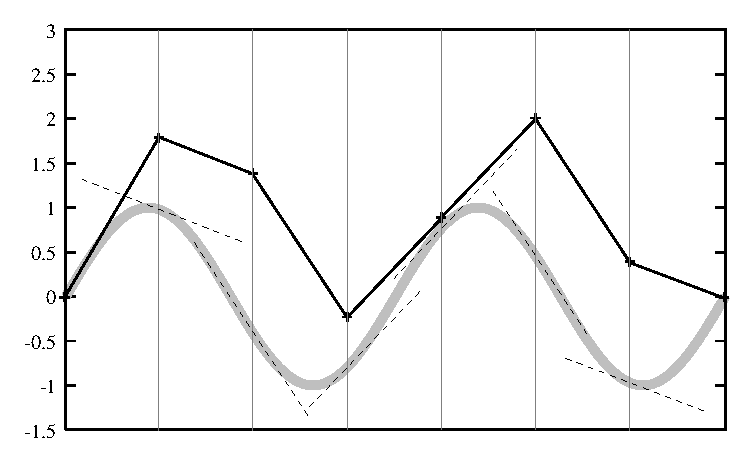
\includegraphics{figures/euler}}
\caption{Demonstration of Euler's method for solving the ODE of simple harmonic oscillation.
    The broad grey line represents the exact solution. At each time step, the method takes the
    derivative (gradient) of the function and uses it to extrapolate linearly.\label{eulersMethod}}
\end{figure}

The general scheme for numerical ODE solvers is to take the value of a function $f(t')$ and its
derivative $\frac{\diff f}{\diff t}(t')$ at some point in time $t'$. From these the algorithm
extrapolates what the value of the function is expected to be some time step $h$ later. The
simplest, most frequently-quoted and worst algorithm for this purpose is Euler's method,
\begin{equation}
f(t'+h) = f(t') + h\frac{\diff f}{\diff t}(t'),
\end{equation}
which performs linear extrapolation. Figure~\ref{eulersMethod} illustrates its operation. The
errors become smaller for tiny time steps, but the method still has a tendency of gaining energy
and is therefore unreliable.

\section{Quaternions\label{quaternions}}
\subsection{The need for Quaternions}
Besides its position, every rigid body in 3D space may have an orientation, in which there are
three degrees of freedom (three independent axes to rotate about).
While the position of a body can be neatly represented using Cartesian coordinates, there is
no obvious best way of describing an orientation. The most common schemes describe
it in terms of a rotation operation which transforms a vector in the body's local
coordinates into world coordinates (or \textsl{vice versa}). But again, there are various different
approaches to representing this rotation, all of which have advantages and disadvantages.

\emph{Euler angles} are probably the most intuitive representation of a 3D rotation, describing
it as a series of three rotations about different axes. These axes are fixed by convention, so it
suffices to specify the three angles of rotation. However, this scheme has a number of
drawbacks~\cite{Saunders:PhD,Shoemake:85}: amongst other things, it is possible that rotation
about one of the axes freezes during an animation (``Gimbal lock'').

\emph{Rotation matrices} are commonly used because they are well understood, easily generalize
to higher dimensions and allow efficient combination with other linear transformations (scaling
and shearing~-- also translation if homogeneous coordinates are employed). However, ODEs over
rotation matrices are difficult to implement correctly, since this representation uses nine
numbers (a $3\times3$ matrix) to represent three degrees of freedom, thus introducing six
additional side conditions which must be maintained. Not doing so causes skew through numerical
drift~\cite{Saunders:PhD}.

\emph{Quaternions}~\cite{Shoemake:85,Eberly:01,MathWorld:Quaternion} are a popular alternative
to the two previous schemes, and they are used extensively in this project.

\subsection{Definition and properties}
Mathematically, quaternions can be regarded as numbers with one real part and three
distinct imaginary parts:
\begin{equation}
\q{q} = q_w + q_x\qi + q_y\qj + q_z\qk
\end{equation}
where $q_w$, $q_x$, $q_y$ and $q_z$ are real numbers and \qi{}, \qj{} and \qk{} satisfy
\begin{equation}
\qi^2 = \qj^2 = \qk^2 = \qi\qj\qk = -1.
\end{equation}
From this follows that
$\qi\qj = -\qj\qi = \qk$ and
$\qj\qk = -\qk\qj = \qi$ and
$\qk\qi = -\qi\qk = \qj$.
Note that multiplication is not commutative.

We will also need the conjugate and the inverse of a quaternion. In analogy to
complex numbers, these are given respectively by
\begin{eqnarray}
\overline{\q{q}} & = & q_w - q_x\qi - q_y\qj - q_z\qk\\
\q{q}^{-1} & = & \frac{\overline{\q{q}}}{\norm{\q{q}}^2}\\
\mathrm{where}\quad&& \norm{q_w + q_x\qi + q_y\qj + q_z\qk} =
    \sqrt{q_w^2 + q_x^2 + q_y^2 + q_z^2}
\end{eqnarray}

Sometimes we will need to relate a 3D vector to a quaternion with zero real part.
For a given vector $\ve{u} = (u_1, u_2, u_3)^T$ we define the corresponding
quaternion to be
\begin{equation}
\label{vectorToQuat}
\tilde{\ve{u}} = u_1\qi + u_2\qj + u_3\qk.
\end{equation}

The complex constants \qi{}, \qj{} and \qk{} are required for the algebra
only, therefore we can represent a quaternion as four numbers $(w,x,y,z)$. It turns out that a
quaternion with unit magnitude ($\norm{\q{q}} = 1$) neatly represents an arbitrary rotation in
3D space, similarly to the way that an ordinary complex number represents a rotation in the 2D
Argand diagram. The condition $\norm{\q{q}} = 1$ reduces the number of degrees of freedom to
three, as required.

Every unit quaternion represents a rotation of angle $\theta$ about an arbitrary axis.
If the axis passes through the origin and has a direction given by the vector
\ve{a} with $\norm{\ve{a}} = 1$, the quaternion describing this rotation is
\begin{equation}
\label{quatRotation}
\q{q} = \cos\left(\frac{\theta}{2}\right) + \tilde{\ve{a}} \sin\left(\frac{\theta}{2}\right).
\end{equation}
It can easily be verified that this quaternion always has unit magnitude. It shall be assumed
throughout this project that the rotation thus described is clockwise (as seen when looking in
the direction of the vector $\ve{a}$) in a right-hand coordinate system, i.e.\ that it is
given by the ``right-hand rule''.

Two rotations can be concatenated by multiplying their quaternions together. The order in which
these rotations are applied is significant, and quaternion multiplication is not commutative,
so the semantics match. The operations are, however, associative. The quaternion product is
obtained simply by multiplying out the components, observing the rules for multiplying \qi{},
\qj{} and \qk{}:
\begin{eqnarray}
\lefteqn{(p_w + p_x\qi + p_y\qj + p_z\qk)(q_w + q_x\qi + q_y\qj + q_z\qk) = } \nonumber\\*
&& (p_w q_w - p_x q_x - p_y q_y - p_z q_z) + 
   (p_w q_x + p_x q_w + p_y q_z - p_z q_y) \,\qi + \nonumber\\*
&& (p_w q_y + p_y q_w + p_z q_x - p_x q_z) \,\qj + 
   (p_w q_z + p_z q_w + p_x q_y - p_y q_x) \,\qk \label{quatProduct}
\end{eqnarray}

To rotate a vector $\ve{v} = (v_1, v_2, v_3)^T$ by a quaternion \q{q}, we first
convert it into its corresponding quaternion $\tilde{\ve{v}}$ as defined in
equation~\ref{vectorToQuat} and then calculate the quaternion product
\begin{equation}
\label{quatTransform}
\tilde{\ve{v}}' = \q{q}\tilde{\ve{v}}\q{q}^{-1}
\end{equation}

If we expand this formula, we find that the real part of the result is always zero, and
that the rotated vector $\ve{v}' = (v_1', v_2', v_3')^T$ corresponds
to $\tilde{\ve{v}}'$ (i.e.\ $\ve{v}'$ is contained in the three complex parts of
the quaternion product).

Some authors, notably Shoemake~\cite{Shoemake:85}, choose to define the product in
equation~\ref{quatTransform} in
the reverse order. The choice is a matter of convention, since it merely changes the effect
of this operation from being a clockwise to a counter-clockwise rotation. I chose the clockwise
convention because it is consistent with the usual definition of the angular velocity vector
in physics.

Observe that under this convention, if \q{q} is itself a product of quaternions
$\q{q} = \q{q}_n \q{q}_{n-1} \cdots \q{q}_1$, the result is that of first applying the
$\q{q}_1$ rotation, then $\q{q}_2$ etc. In other words, the rotations in a quaternion product
are applied from right to left. To verify that this is the case, the identity
$\overline{\q{p}\, \q{q}} = \q{\overline{q}}\; \q{\overline{p}}$
is useful~\cite{MathWorld:Quaternion}.

\subsection{Quaternion integration}

We have seen that given the torques on a body, a numerical ODE solver can treat each component
of the vector separately to obtain the new angular momentum. Now that we are representing
orientation as a quaternion, how do we compute the change in orientation given the body's angular
velocity?

The instantaneous rate of change of a quaternion \q{q} over time is
usually~\cite{BaraffWitkin:97,Eberly:04,Saunders:PhD} given as
\begin{equation}
\label{quatRateOfChange}
\dot{\q{q}}(t) = \frac{1}{2}\tilde{\ve{\omega}}(t)\q{q}(t)
\end{equation}
where $\tilde{\ve{\omega}}$ is the quaternion corresponding to the angular velocity
vector $\ve{\omega}$. The quaternion $\dot{\q{q}}$ can be fed into an ODE solver which can handle
its four components separately. However, when this is done it is observed that the new orientation
$\q{q}'$ no longer has unit magnitude. This is an inherent property of the definition in
equation~\ref{quatRateOfChange}, and not, as sometimes claimed~\cite{Eberly:04}, merely a matter
of numerical round-off (proof in appendix~\ref{quatIntegrationMagnitude}). Usually this problem
is `solved' by normalizing the quaternion:
\begin{equation}
\q{q}(t + h) = \frac{\q{q}'}{\norm{\q{q}'}} \quad\quad\mathrm{where}\quad
    \q{q}' = \q{q}(t) + h\dot{\q{q}}(t)
\end{equation}
(using Euler's method for clarity; $\q{q}'$ would be appropriately redefined when using e.g.\ RK4).
This `solution' seemed quite \textsl{ad hoc} to me, and I indeed showed that it returns a
completely wrong result if the angular velocity is large (see appendix~\ref{quatNormalization}).

To obtain the correct result, the ODE solver must be modified. Whenever it calculates the sum of
a quaternion and a scaled derivative, as in $\q{q}(t) + h\dot{\q{q}}(t)$, we replace the summation
by $\mathrm{Quergs}(\q{q}(t), h\dot{\q{q}}(t))$, where $\mathrm{Quergs}$ is the
\emph{Qu}at\emph{er}nion inte\emph{g}ration \emph{s}tep\footnote{This naming follows the spirit of
Shoemake~\cite{Shoemake:85}, whose ``Slerp'' function is an `acronym' of \emph{S}pherical
\emph{l}inear int\emph{erp}olation.}:
\begin{equation}
\label{quergs}
\mathrm{Quergs}(\q{q}, \Delta\q{q}) =
    \frac{\q{q} + \tan\left(\norm{\Delta\q{q}}\right)
        \frac{\Delta\q{q}}{\norm{\Delta\q{q}}}}{
    \sqrt{\norm{\q{q}}^2 + \tan^2\left(\norm{\Delta\q{q}}\right)}}
\end{equation}

This formula is derived in appendix~\ref{quatIntegrationDerivation} and applied to the RK4
algorithm in appendix~\ref{quergsRK4}. It ensures that the resulting quaternion has unit magnitude
and is correct even at high velocities. I have not come across anything like it in the literature
I have searched, and hence have some grounds to believe it may be new.

\section{Articulated bodies\label{articulatedBodies}}

\subsection{Approaches to constraints\label{approachesToConstraints}}
The methods developed so far allow the simulation of a single rigid body with forces
acting on it. Further challenges arise when we consider multibody systems in which there are
conditions which must not be violated. In an articulated body, for example, each segment
must be modelled as an invidiual rigid body, under the condition that joints must not be pulled
apart.

There are various strategies for simulating articulated bodies:

\begin{itemize}
\item \emph{Penalty methods} conceptually join bodies together with springs so that when they
    begin to separate, a restoring force causes them to move back together again. These methods
    are simple to implement initially but hard to get right: if the springs are too weak, the
    bodies will separate too far; if they are too stiff, very large forces can arise suddenly,
    causing the simulation to become unstable.

\item Mechanics formulations using \emph{generalized coordinates}
    \cite{Hand:98,Goldstein:80,Featherstone:87,Wilhelms:91} build constraints firmly into
    the system: the number of generalized coordinates equals the actual number of degrees of
    freedom after the constraints have been applied. The state of the system is specified only in
    terms of these generalized coordinates, and they are chosen such that the system will always
    be in a legal state, irrespective of what the values of the coordinates are. These algorithms
    allow efficient and reliable computation. However, the equations are only tractable for
    so-called \emph{holonomic constraints} (definition in~\cite{Hand:98}), which excludes
    many interesting systems.

\item This project makes a compromise between the flexibility of penalty methods and the stability
    of generalized coordinates. As in the penalty method, we initially treat each segment of an
    articulated body separately. The constraints are then formulated in such a way that we can
    not only tell whether the system is currently in an illegal state, but also whether it is
    moving towards one, and even whether it is accelerating towards one. Using the method of
    \emph{Lagrange multipliers} we can determine what forces must be applied to the bodies to
    nullify this unwanted acceleration before it ever occurs. This compromise comes at the
    expense of higher computational cost, because systems of linear equations have to be solved
    at run-time.
\end{itemize}

The mathematical formulation of Lagrange multipliers is derived in~\cite{BaraffWitkin:97} and
extended in~\cite{Saunders:PhD} (also see~\cite{Baraff:96} for an optimized algorithm),
and I only state the results here.


\subsection{Lagrange multipliers\label{lagrange}}

Each constraint effectively reduces the number of degrees of freedom by one, and is expressed
as a function $c$ which is zero when the constraint is satisfied. (A ball-and-socket
joint, which allows three modes of rotation but no separation, reduces the number of d.o.f.\ by
three and is therefore expressed as a vector of three scalar constraint functions.) All constraint
functions can then be concatenated into a single constraint vector \ve{c}.

The constraints can be satisfied by solving the equation\footnote{Here the sign convention
of~\cite{BaraffWitkin:97} is adopted, which is the opposite of~\cite{Saunders:PhD}.}
\begin{equation}
\label{lagrangeEquation}
-\m{J}\m{M}^{-1}\m{J}^T\ve{\lambda} = \dot{\m{J}}\dot{\ve{x}} +
    \m{J}\m{M}^{-1}(\ve{\Phi} + \ve{\Phi}_p) + k\ve{c} + d\dot{\ve{c}}.
\end{equation}
The values of all variables except for the vector $\ve{\lambda}$ in this equation are
known, and they are explained in appendix~\ref{constraintPrerequisites}. In brief, they are:

\vspace{10pt}
\begin{tabular}{@{}ll}
\ve{c}, $\dot{\ve{c}}$ & Constraint vector and its first derivative w.r.t.\ time.\\
\m{J}, $\dot{\m{J}}$ & Jacobian matrices derived from \ve{c} (see appendix~\ref{jacCalculation}).\\
\m{M} & Mass-inertia matrix combining the masses and moments of inertia\\
      & of all bodies in the scene. \\
$\dot{\ve{x}}$ & Combined linear and angular velocity vector of all bodies.\\
\ve{\Phi} & Combined forces and torque vectors acting on all bodies.\\
$\ve{\Phi}_p$ & Effects of free precession.\\
$k$, $d$ & Scalar constants regulating error compensation, discussed
    in~\cite{BaraffWitkin:97}.
\end{tabular}
\vspace{10pt}

For us it will suffice to consider this equation to be a `black box' which can be
given to a linear equation solver to obtain $\ve{\lambda}$.

$\ve{\lambda}$ is an $m$-row vector of so-called \emph{Lagrange multipliers} (after which this
algorithm is named), where $m$ is the number of constraints. Once we have solved for it, we can
compute the expression
\begin{equation} \label{lagrangeSolution}
\ve{\Phi}_c = \m{J}^T\,\ve{\lambda}.
\end{equation}
$\ve{\Phi}_c$ is the vector of constraint restoring forces and torques for all bodies.
Speaking in physical terms, these are the reaction forces which balance the action \ve{\Phi}.
All we therefore need to do is to compute $\ve{\Phi} + \ve{\Phi}_c$ and to feed the result into
our ODE solver, and the motion which ensues will satisfy the constraints.
$\ve{\Phi}_p$ must not be added to this term\footnote{provided the moments of inertia are
recalculated based on the bodies' orientation at every time step.}.


\subsection{Modelling the human body}

The human body's selection of joint types is quite limited compared to the range of connectors
found in machines~\cite{Kalra:95}: for example, there are no sliding joints or screws. The simple
types of joint found in human bodies are ball-and-socket joints allowing rotation about three axes
(like shoulders and hips), and revolute joints limited to a single axis (like knees and elbows).
The issue is made more complicated by compound joints like the spine, and motion which occurs
along the length of a segment rather than at a joint (like rotating the wrist about the axis of
the lower arm, which occurs through a relative shift of the ulna and radius
bones~\cite{Anatomy:03}).

To make the model manageable, I chose to be anatomically ignorant and assumed that two adjacent
segments of an articulated body are connected by a single joint, and that rotation occurs only
about this joint. Each bone has a local coordinate system whose origin lies at the joint to the
parent bone. This is illustrated in figure~\ref{jointsFigure}.

\begin{figure}
\centerline{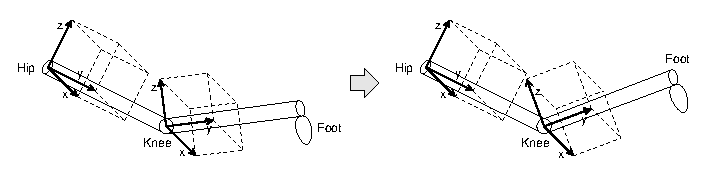
\includegraphics{figures/joint1}}
\caption{Two bones connected by a revolute joint, e.g.\ a knee. Rotation is constrained to be
    possible only about the local x~axis of the knee, but not the local y~axis
    (the lower leg itself) or the local z~axis (sideways).\label{jointsFigure}}
\end{figure}

There are different ways of formulating this model. My approach is to assume initially that every
joint is a ball-and-socket type. For those joints which are not not, additional constraints are
added to restrict the permitted axes of rotation.

\subsection{Ball-and-socket joints}

The position of a joint is a particular offset from the centre of mass in one body's frame, and a
different offset from the other body's centre of mass. While the bodies may move around, these
offsets stay constant (as seen in the body's frame).

Figure~\ref{ballAndSocketFigure} gives an example: here, the configuration of bodies satisfies the
ball-and-socket constraint iff $\ve{a}+\ve{s} = \ve{b}+\ve{t}$, i.e.\ if the joint has not
separated. We can rewrite this to give the constraint function
\begin{equation}
\ve{c} = \ve{a} + \ve{s} - \ve{b} - \ve{t}
\end{equation}
which equals \ve{0}, the three-dimensional null vector, iff the constraint is satisfied.

\begin{figure}
\psfrag{frag:o}{\ve{O}}
\psfrag{frag:a}{\ve{a}}
\psfrag{frag:b}{\ve{b}}
\psfrag{frag:s}{\ve{s}}
\psfrag{frag:t}{\ve{t}}
\centerline{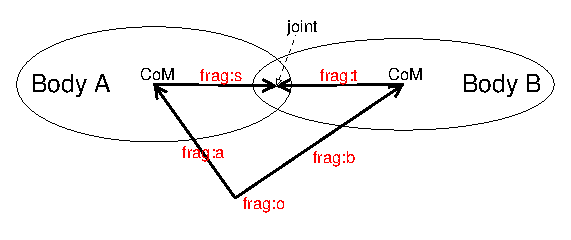
\includegraphics{figures/joint2}}
\caption[]{A valid ball-and-socket joint configuration. \ve{s} is constant in body~A's frame,
    while \ve{t} is constant in the frame of body~B. In the world frame, these two vectors
    therefore rotate according to their respective body's orientation.\label{ballAndSocketFigure}}
\end{figure}

\subsection{Rotation constraints\label{rotationConstraints}}

In the case of an elbow or a knee, we also need to prohibit the rotation about particular axes.
After some thought I came up with the constraint function
\begin{equation}\label{rotationConstraintEqn}
c = \Re(\tilde{\ve{n}}\q{p}^{-1}\q{q})
\end{equation}
in which \q{p} is the quaternion of orientation for body~A, \q{q} the quaternion for body~B, and
\ve{n} a vector pointing along the prohibited axis in body~A's frame. Setting $c$ to zero ensures
that no rotation occurs about the axis~\ve{n}. If two different axes are prohibited with two
separate constraints, then rotation is only possible about a single axis orthogonal to the two
prohibited axes. Further details on this constraint are given in appendix~\ref{constrJoystick}.

\subsection{Angle limitation\label{angleLimitation}}

The constraints described so far capture most of the features of the human skeleton, with one
exception: if rotation is permitted about some axis, there is no limit to the amount of rotation
that can occur. For example, permitting Alfred to look left and right would allow the simulation
to rotate his head by an arbitrary amount. Imposing
limits on the angle of rotation as well as the axis is possible but more complicated, and will
be explained in section~\ref{generalizedCollisions}. It is worth noting that this is our
first example of a non-holonomic constraint, and thus lies beyond the capabilities of
generalized-coordinate approaches.

\section{Software preparation\label{softwarePreparation}}

\subsection{Data structures and file formats}
Two types of data files are mainly used in this project: an input file, specifying the bodies,
their geometry and initial configuration in a scene, and an output file for the simulation
results.

\subsubsection{Input data}
The input data has a graph structure which is visually represented in figure~\ref{sceneSchema}.
Geometric objects are represented as \emph{meshes} of triangles. Each triangle (or \emph{face})
of the object's surface is delimited by three \emph{vertices}. This simple structure is sufficient
to represent a great variety of shapes, and although a large number of vertices is necessary to
adequately approximate curved surfaces, the ease of handling this data outweighs the costs caused
by its quantity.

\begin{figure}
\centerline{\scalebox{0.35}{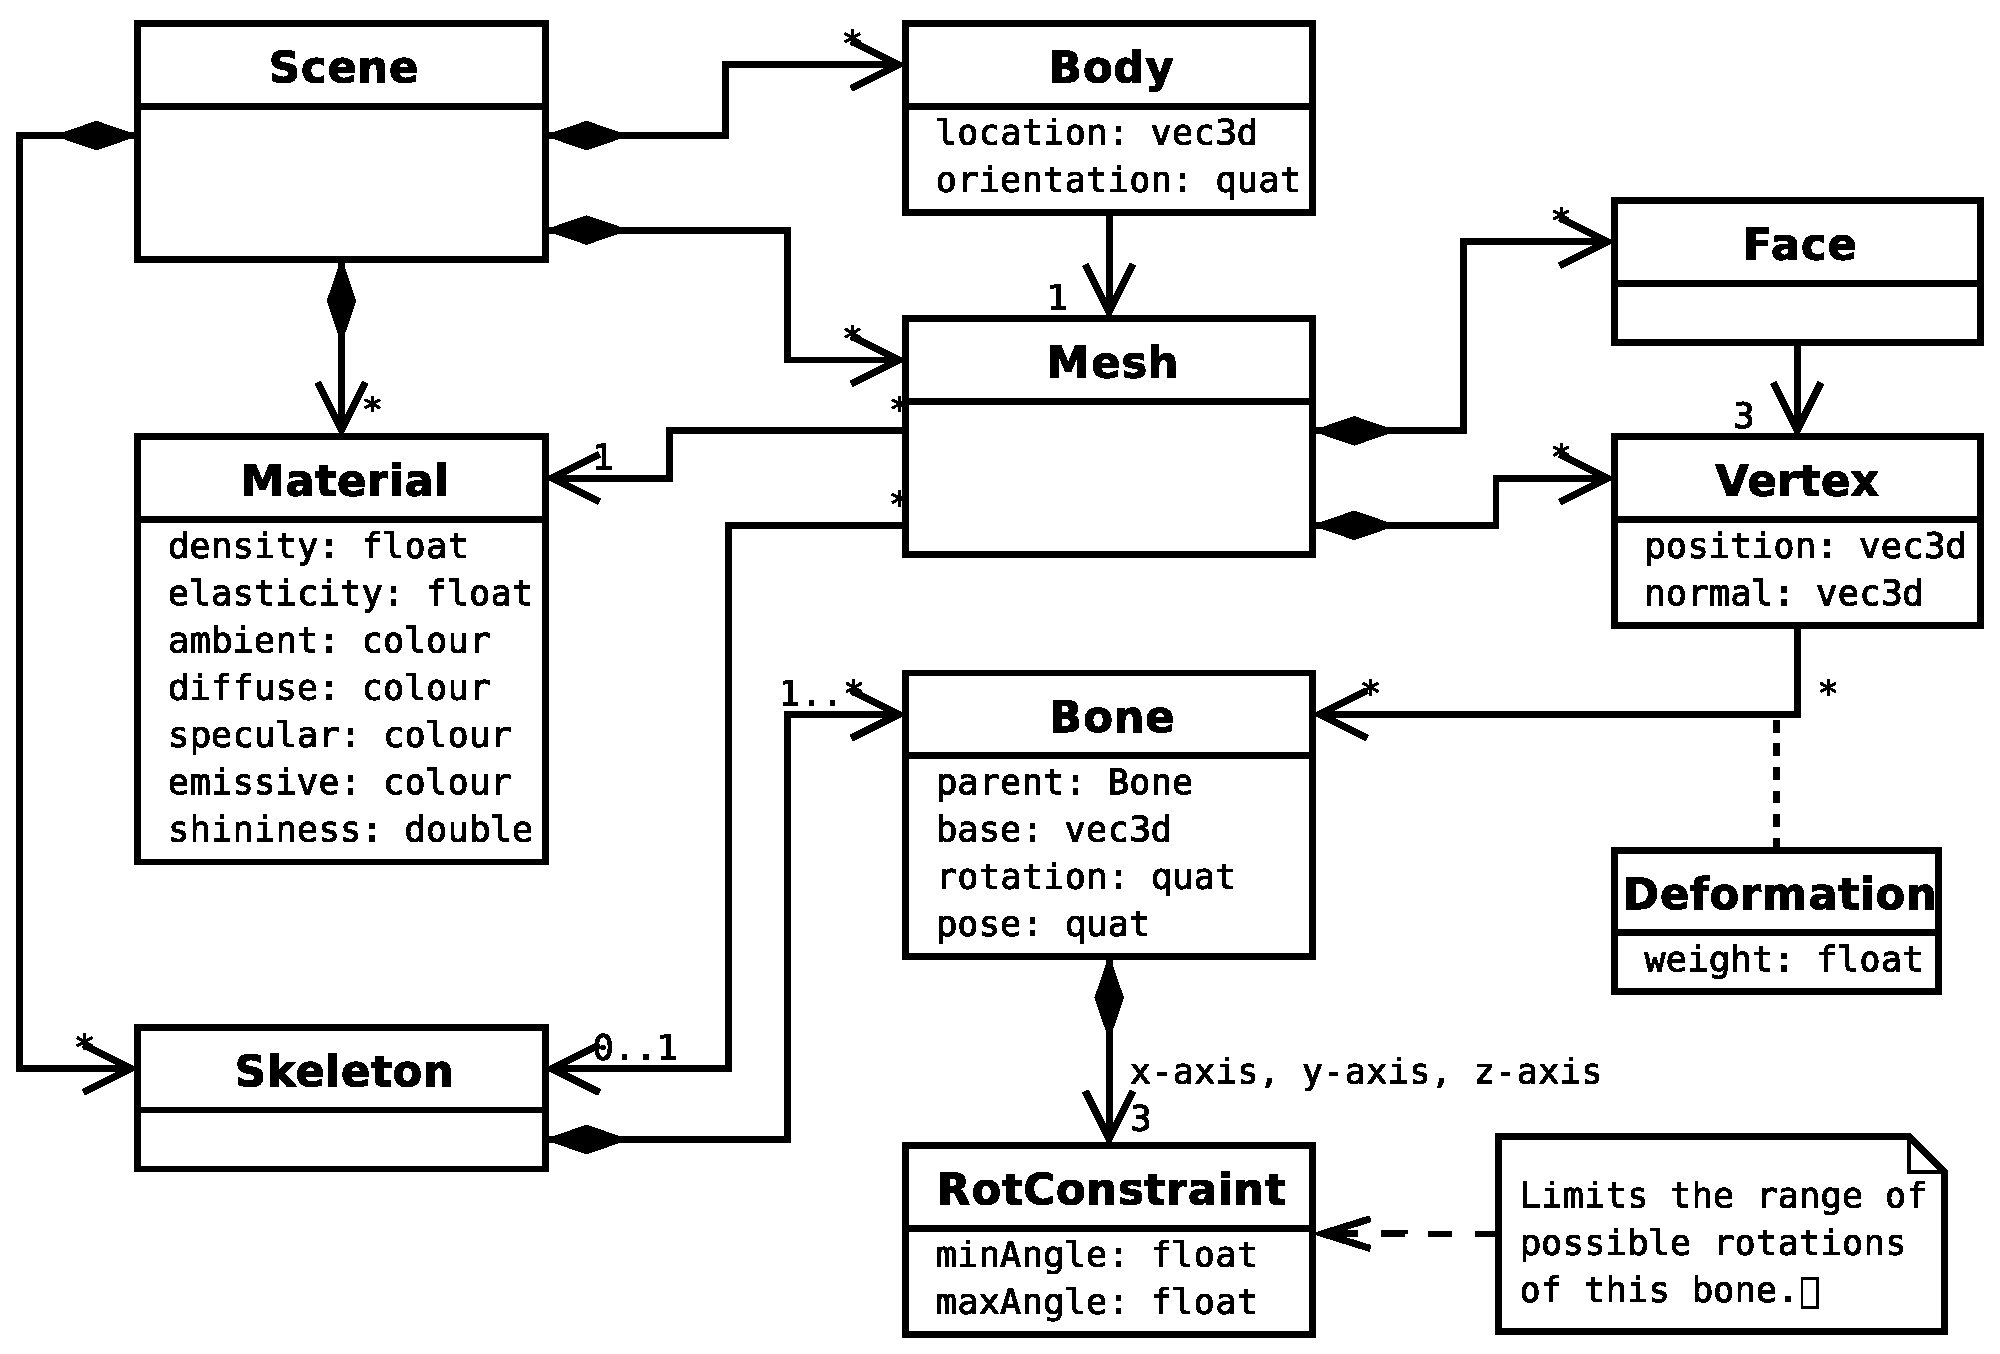
\includegraphics{figures/schema}}}
\caption{Structure of the input data to a simulation, using UML syntax.\label{sceneSchema}}
\end{figure}

Several \emph{bodies} in the scene may share the same mesh if they are identical up to rotation
and translation. A mesh is also associated with a \emph{material} which is used to determine the
visual rendering (colour) and the physical behaviour (density, elasticity).

If the scene contains articulated bodies, \emph{skeletons} must be defined in the file. A skeleton
is a tree of \emph{bones} in which each bone has an offset and a rotation relative to its parent.
If one bone~-- say an upper arm~-- in this structure moves while all other relative rotations stay
unchanged, then all children of this bone~-- up to the tip of the little finger~-- will be rotated
equally. This matches the natural behaviour of a skeleton. There can also be limits on the maximum
angles of rotation for each bone; these are discussed in more detail later.

In an articulated mesh, each vertex is associated with one or more bones of a particular skeleton.
Normally it will be associated with one bone, but a weighted sum of two or even three adjacent
bones' transformations may be used to create the illusion of smoothly deforming joints. Hence it
is not possible to completely decompose an articulated body into its individual limbs, but the
articulated mesh must be treated as a whole.

Since this data structure is designed to be very general-purpose, I wanted to use a file format
which could easily be generated by 3D modelling applications or manually edited. I chose to use
\textsl{XML}\footnote{eXtensible Markup Language, \texttt{http://www.w3.org/XML/}} as a basis
since it is easy to read both by humans and by \textsl{XML} parsing libraries. I could not
find a format which suited my needs~-- all existing formats are either far too complicated or not
powerful enough~-- and therefore designed a custom schema. I also created an
\textsl{XSLT}\footnote{eXtensible Stylesheet Language with Transformations,
\texttt{http://www.w3.org/TR/xslt}} stylesheet which semi-automatically converts the
\textsl{Cal3D}\footnote{Character Animation Library file format, \texttt{http://cal3d.sourceforge.net/}}
format into input data for this project. \textsl{Cal3D} can be exported by \textsl{Blender}
(see below).

\subsubsection{Output data}
The output of a simulation is much simpler than the input data: All that is required is the
position and orientation, and possibly the velocities, of each body at each time step. For
articulated bodies, the orientation of each bone is also required. This suggests a simple
matrix layout in which bodies and bones are sorted along one dimension and time along
the other.

The output file is such a matrix, arranged in a simple \textsc{ascii} file format which can
directly be imported by \textsl{Octave} (see below). \textsl{Octave} can then be used for further
processing or evaluation of the results.

\subsection{Tools}
\subsubsection{Programming languages}
I chose \textsl{Java~1.5}\footnote{Using Sun's J2SE JDK~5.0, \texttt{http://java.sun.com/}}
as language for the implementation of the bulk of the project. Java's strictly object-oriented
paradigm and its package concept facilitate the management of large software engineering
projects; it is mature, well supported and benefits from an extensive run-time library. I
particularly appreciate its good type safety (and hence bug prevention) compared to languages
like C and make heavy use of the \emph{generic} type polymorphism added in version~1.5.

Java is a very verbose language though, so I decided that it would be beneficial to prototype
the algorithmically tricky parts in a concise scripting language first. For this I used
\textsl{GNU Octave}\footnote{GNU Octave~-- \texttt{http://www.octave.org/}~-- uses a language
mostly compatible to \textsc{Matlab}~-- \texttt{http://www.mathworks.com/products/matlab/}},
which is optimized for numerical matrix and vector-based computation. I implemented nearly all
numerical algorithms in this project in \textsl{Octave} first; this version was too slow to be
of much practical use, but was extremely useful to guide the subsequent Java implementation.
Octave was also used for processing of simulation output, for example to generate plots of the
simulation behaviour.

\subsubsection{Libraries}
Rendered output is specified in the project requirements, and the most common choice for
displaying 3D graphics in Java programs is the
\textsl{Java3D}\footnote{\texttt{https://java3d.dev.java.net/}} library. \textsl{Java3D} provides
a clean object-oriented interface to either a software renderer or accelerated graphics hardware,
and is also quite well documented.

Processing of the input file was done using an \textsl{XML data-binding tool} which I had
developed independently in summer 2005. This tool takes a grammar for an \textsl{XML} schema in
\textsl{RELAX NG}\footnote{\texttt{http://www.relaxng.org/}} format and generates a set of
Java classes implementing a run-time representation of that schema. The actual low-level parsing
is done by the \textsl{SAX}\footnote{Simple API for XML, \texttt{http://www.saxproject.org/}}
parser implementation in \textsl{Xerces}\footnote{Apache Xerces2 Java,
\texttt{http://xerces.apache.org/xerces2-j/}}.

Some of the numerical algorithms required by the simulation could have been obtained through
libraries. However, none of them are particularly complicated~-- their C implementation
in~\cite{NRinC} is at most a few pages long and is easy to translate into Java. I therefore chose
to implement the algorithms myself, giving me the freedom to incorporate enhancements like
equation~\ref{quergs}.

\subsubsection{Tool chain}
For Java development, the \textsl{Eclipse}\footnote{\texttt{http://www.eclipse.org/}} was set up,
and a dual build system using the \textsl{Ant}\footnote{\texttt{http://ant.apache.org/}} tool
was kept as fallback in case there were problems with \textsl{Eclipse}. To profile the Java
implementation, \textsl{EJP}\footnote{Extensible Java Profiler, \texttt{http://ejp.sourceforge.org/}}
was used.

I created input data for the simulation using \textsl{Blender}\footnote{\texttt{http://www.blender.org/}},
an open source 3D modelling/animation/rendering application. \textsl{Blender} supports internal
scripting in \textsl{Python}\footnote{\texttt{http://www.python.org/}} to extend its functionality.
This allowed me to write some short \textsl{Python} scripts which imported the results of a
simulation as animation back into \textsl{Blender}, acting on the original models. This was useful
to review simulation results separately from the internal \textsl{Java3D} output. \textsl{Blender}
can also export animations to the \textsl{YafRay}\footnote{\texttt{http://www.yafray.org/}}
raytracer to produce high-quality video files. These AVI files were converted to MPEG-1 video
streams using \textsl{FFmpeg}\footnote{\texttt{http://ffmpeg.sourceforge.net/}}.

Some types of constraint, which will be described later, involve very messy algebraic expressions.
I found it useful to automatically generate optimized source code for these expressions
using \textsl{Maple}\footnote{\texttt{http://www.maplesoft.com/products/maple/}}.

\subsubsection{Backup strategy}
All work was done either on PWF machines or my own computer. All project files were kept under
version control using \textsl{CVS}\footnote{\texttt{http://www.nongnu.org/cvs/}}, and regular
snapshots of the whole repository were transferred to the \textsl{Pelican} backup service.
A working build environment was maintained both on the PWF and my computer so that work could
continue seamlessly in case of desaster.

\subsubsection{Example scenes}
\begin{figure}
\centerline{
    \raisebox{2mm}{\scalebox{0.72}{\includegraphics{figures/alfred-mesh}}}\hspace{1.3cm}
    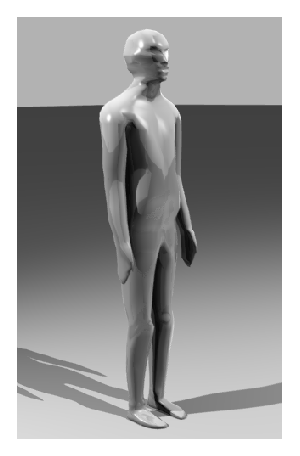
\includegraphics{figures/alfred-rendered}
    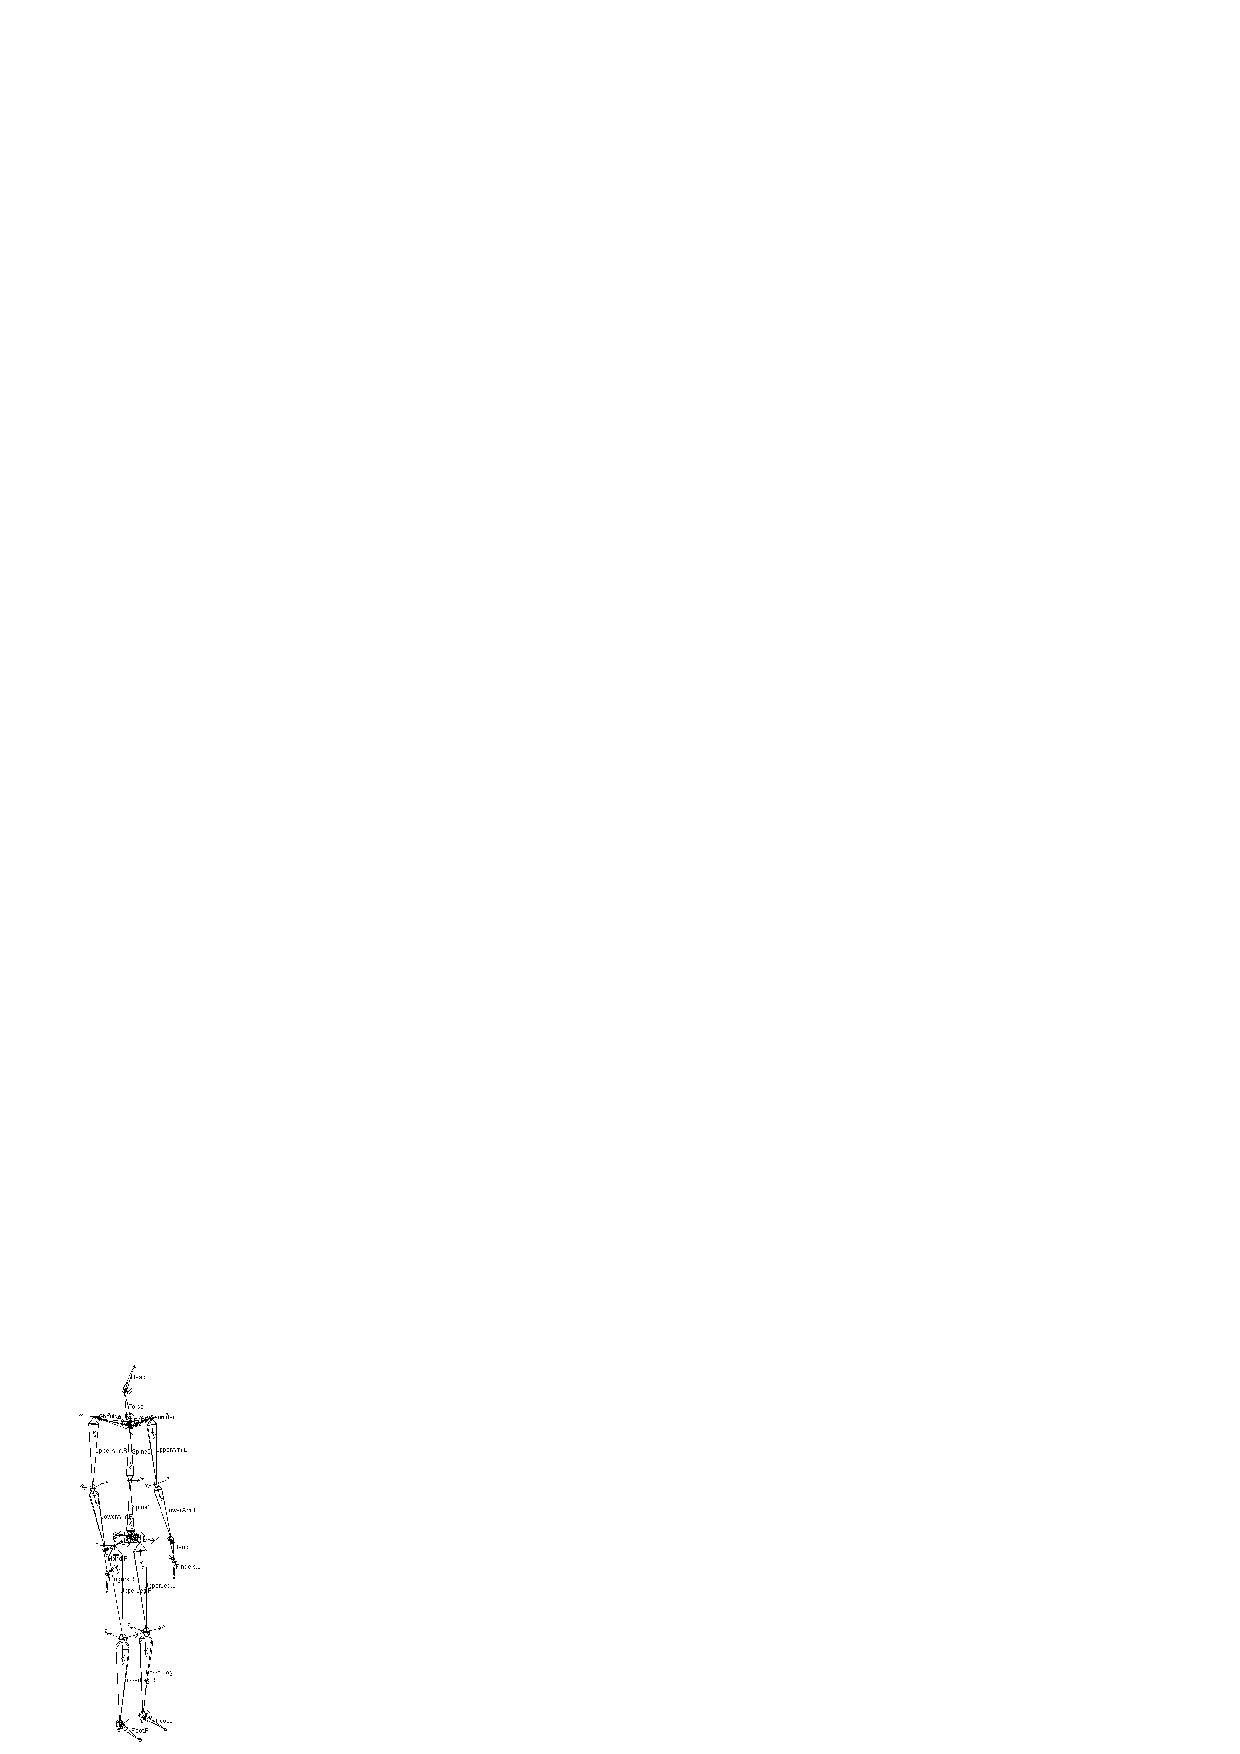
\includegraphics{figures/alfred-skeleton}}
\caption{Alfred, one of the meshes used as input data. From left to right: The triangle mesh in
    wireframe view; a raytraced perspective view; and the skeleton in its rest position.
    \label{alfredFigure}}
\end{figure}
I modelled all input data for the simulations in \textsl{Blender}. The most interesting mesh
is that of \emph{Alfred}, a humanoid articulated body (figure~\ref{alfredFigure}), which I created
using human anatomical data~\cite{Anatomy:03}. It is bound to a skeleton of 25 bones, also shown
in figure~\ref{alfredFigure}. There are some bugs in this mesh~-- for example, strange cracks
appear at the shoulders when the arms are lifted high~-- but since creating good example data
is not a primary objective of this project, these problems should be disregarded.

\chapter{Implementation}
In section~\ref{introOverview}, six core components of this project were identified. The first
three~-- ODE solving, rigid body dynamics and articulated bodies~-- were introduced in the last
chapter. In this chapter I give details of how the whole simulation was implemented in software,
and which challenges I faced along the way (section~\ref{implementation}). I then elaborate on
the three remaining components~-- collision detection (section~\ref{collisionDetection}), and
handling of colliding and resting contacts (section~\ref{collisionHandling}).


\section{Casting theory into code\label{implementation}}

My final implementation comprises 700 lines of \textsl{Octave} code (prototyping and numerical
tools) and 10500 lines of \textsl{Java} code for the main implementation (including 3500 lines
automatically generated by the XML data binding tool), plus a few fragments in other languages.

\subsection{The engineering process\label{engineering}}

The primary management challenge was to control the uncertainties caused by my lack of prior
knowledge of the algorithmic details required. The first four milestones, up to collision
detection, bore no major uncertainties, and could therefore be accomplished on schedule. I started
surveying the options for implementing articulated bodies during milestone~2; at this point I
realized that it was going to be much more challenging than expected, and that I would have to
adapt my strategy.

I decided to suspend coding after milestone~4 and to work on the theory until I was certain that
I understood it. If I tried to implement my ideas immediately, I believe the result would have
been chaotic and a waste of time. I set myself a new hierarchy of tasks arranged in a rectangular
grid. From left to right, the columns were the simulation components as listed in
section~\ref{introOverview} (except for item~4, which was already completed). From top to bottom,
the rows were labelled
\begin{enumerate}
\item search for literature relevant to the subject;
\item read and completely understand it;
\item if it is insufficient and no more literature can be found, work out a new algorithm for
    doing it;
\item argue or prove that the algorithm works correctly;
\item write down a good explanation of the algorithm, as if it were for another person to read, to
    ensure I fully understand it;
\item write a prototype in \textsl{Octave}.
\end{enumerate}

The idea of this grid is that each cell~-- one of these six tasks applied to one of the five
simulation components~-- depends on those above and to the left of it. Thus I could start in the
top left-hand corner and work towards the bottom right-hand corner; backtracking was possible when
I got stuck, but there was a clear objective and I could track progress. I decided that only
once I had covered the whole grid would I lay out and implement the \textsl{Java} program.
Completing the grid took me seven weeks, from mid-December until the end of January.

The \textsl{Java} implementation, testing and debugging were completed in the following seven
weeks~-- due to the thorough planning beforehand, this was slightly less than the nine weeks
originally allocated to this part of the project. Including the seven additional weeks required to
complete the ``theory grid'', the project was now five weeks behind schedule.

Writing the dissertation, again a task with few uncertainties, took the allotted length of time.
With five weeks delay carried over and one week of holiday, the project finished six weeks behind
schedule. Given the early completion date (19~March) originally envisaged, this still
allowed me to submit well before the deadline.


\subsection{Application architecture\label{architecture}}

The \textsl{Java} implementation consists of five packages:

\begin{description}
\item[Scene.] Facilities to load a scene description from an XML input file, and data structures
    to represent it at run-time. This package is automatically generated by the data binding tool.
\item[Maths.] \sloppypar General-purpose implementations of vectors, matrices (including sparse matrices),
    quaternions, solver for ordinary differential equations (variable-step-size Runge-Kutta with
    Cash-Karp parameters~\cite{NRinC}), and a solver for systems of linear equations (biconjugate
    gradient method, also taken from~\cite{NRinC}).
\item[Geometry.] Handling of triangle meshes at run-time: deformation of articulated meshes,
    rendering of meshes using \textsl{Java3D}, collision detection. (Depends on Scene and Maths)
\item[Dynamics.] Implementations of a rigid body and all the different constraint types.
    Architecture for handling interactions between objects. Articulated body code combining
    rigid bodies and constraints, and implementation of the collision/contact handling algorithms.
    (Depends on Scene, Maths and Geometry)
\item[Main.] Main application class and test cases. (Depends on Scene and Dynamics)
\end{description}

The application follows a clean object-oriented design throughout. Some excerpts from its
class/interface hierarchy are shown in figure~\ref{classHierarchy}. This diagram indicates how
extensible the architecture is: any two \textsf{SimulationObject}s can interact, generating an
\textsf{Interaction} object~-- this could be anything from a repulsive Coulomb force to some
sort of sentient behaviour~-- without having to change any of the rest of the system.

\begin{figure}
\centerline{\scalebox{0.4}{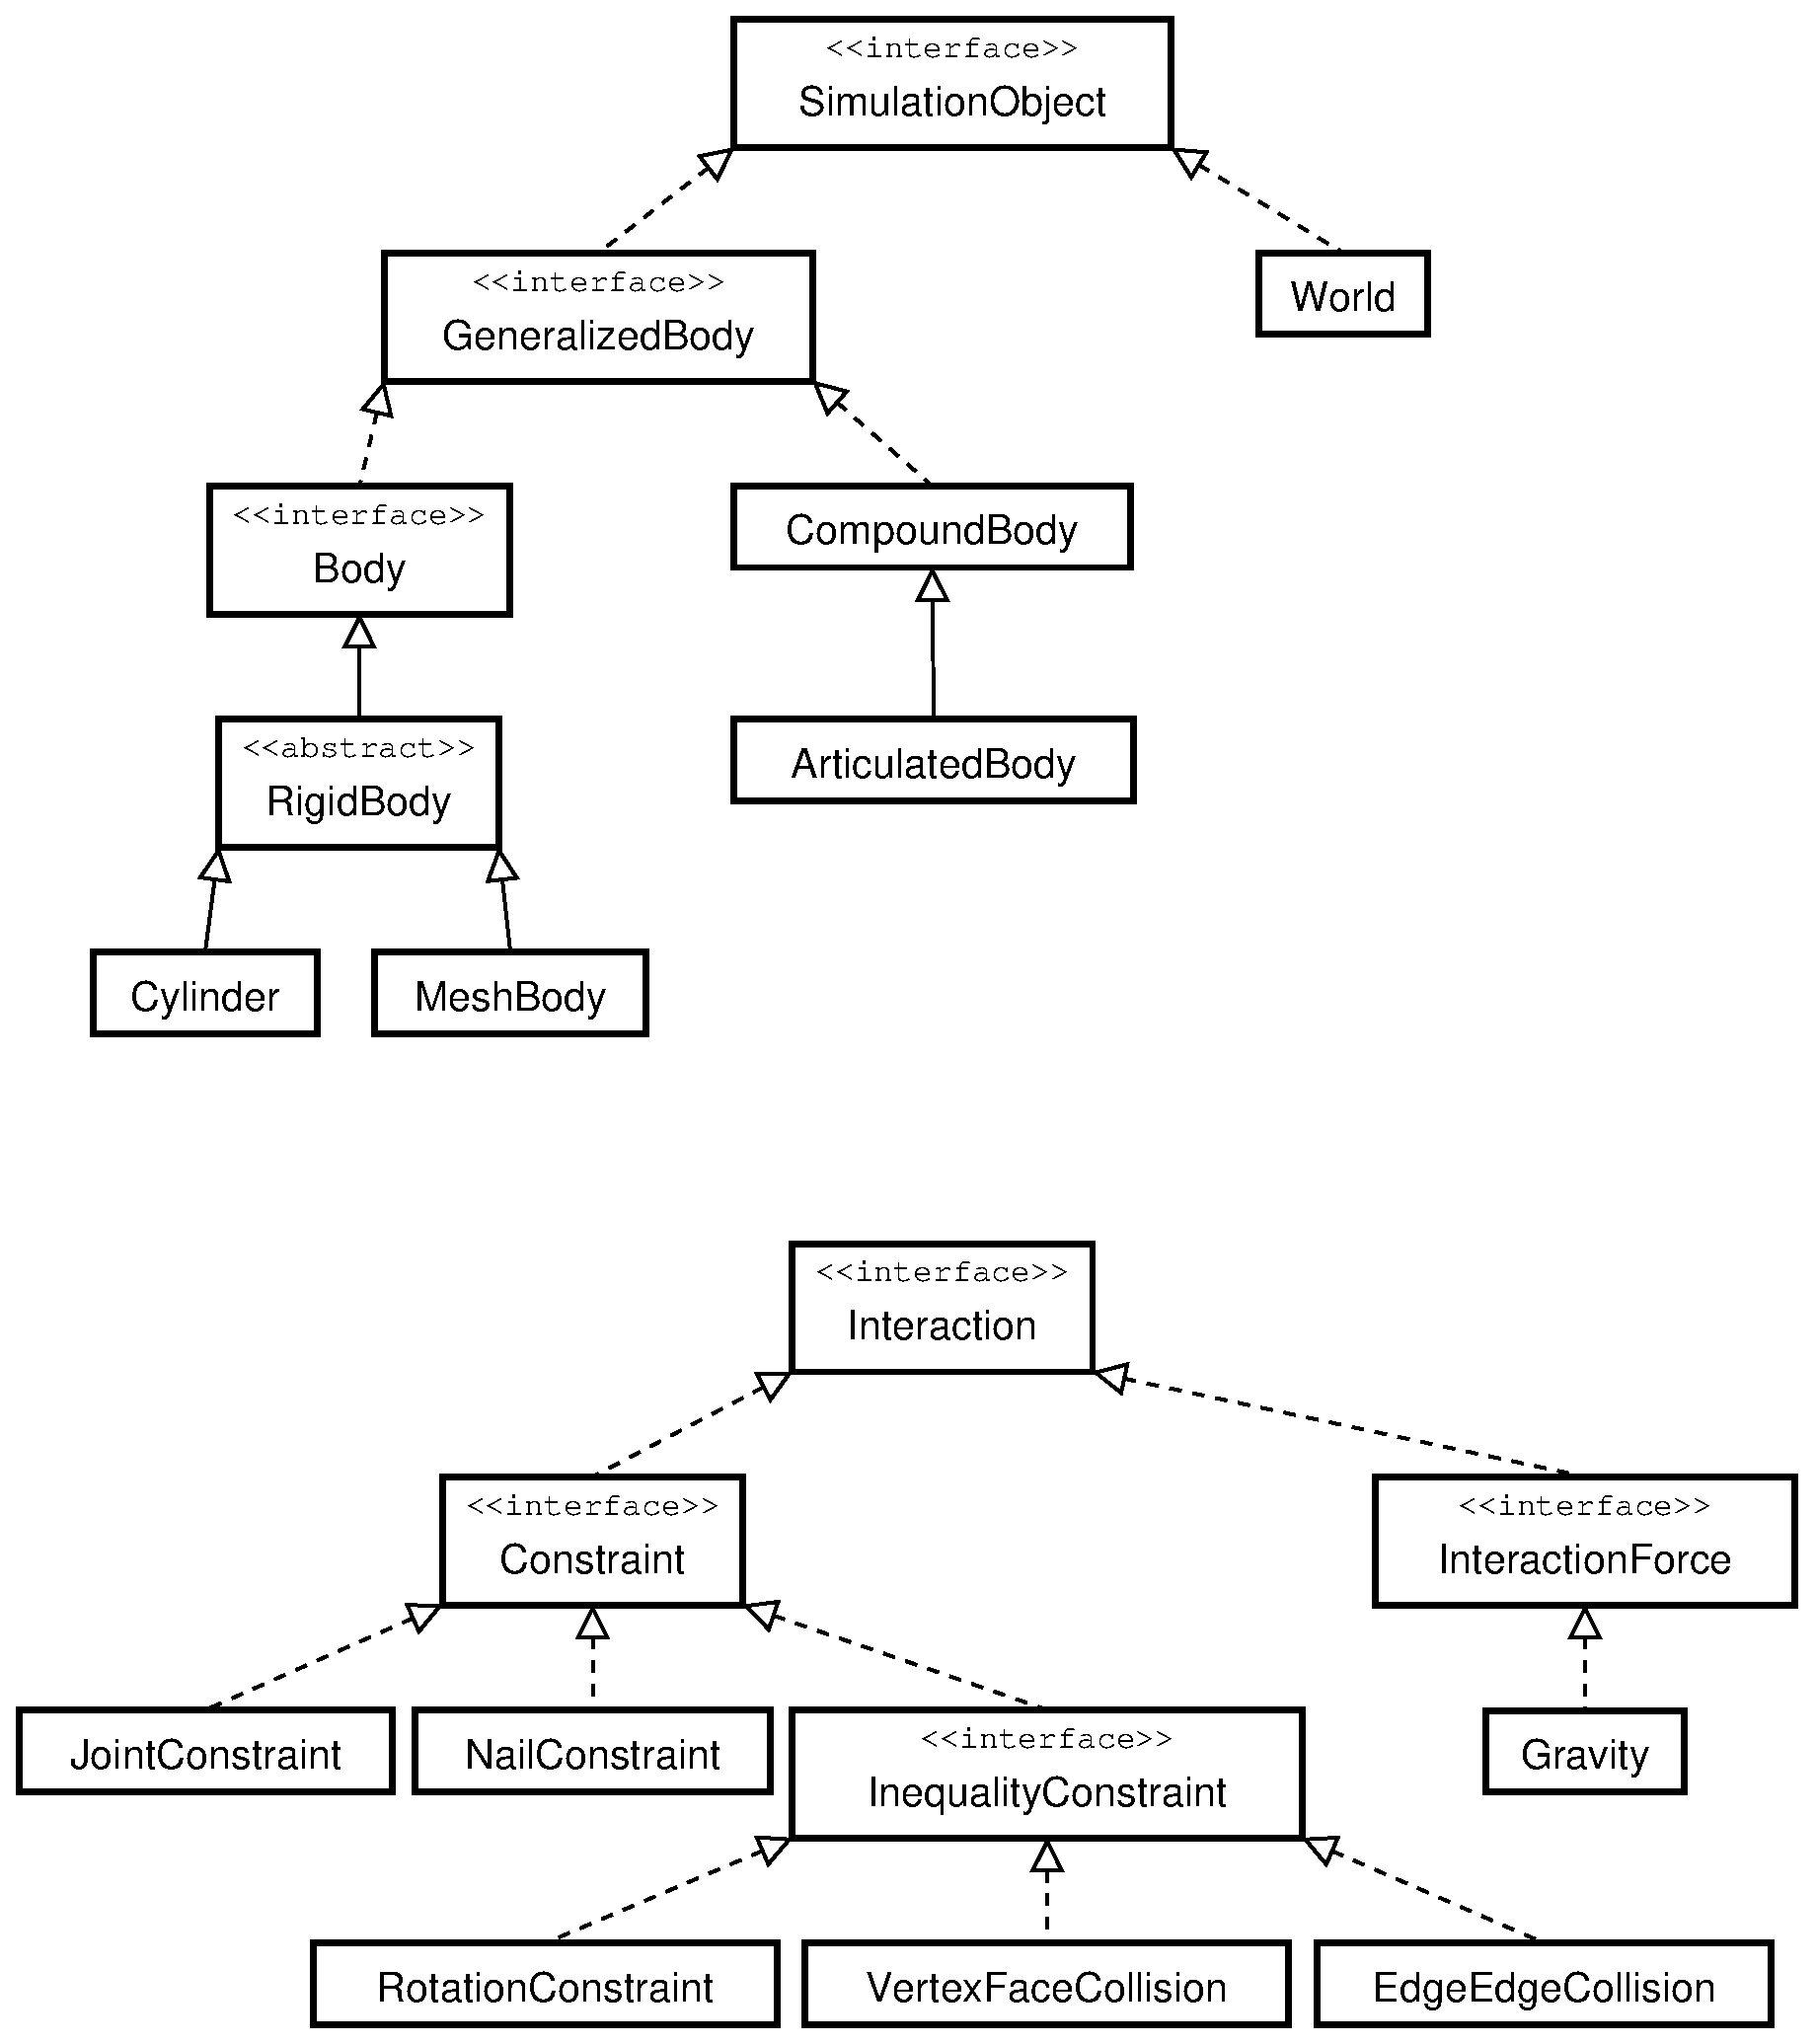
\includegraphics{figures/classes}}}
\caption{Two class inheritance hierarchies from the Dynamics package. Methods are omitted for
    better readability.\label{classHierarchy}}
\end{figure}

This design encapsulates algorithms in a way which is both clear and efficient. To give but two
examples:
\begin{itemize}
\item the ODE solver operates only on the \textsf{Vector} interface. The \textsf{RigidBody}'s
    state vector implements the \textsf{add} method in such a way that quaternions are
    automatically normalized when appropriate. Thus the ODE solver needs to know nothing about
    quaternions, and a \textsf{RigidBody} object can be handled by any ODE solver.
\item the biconjugate gradient method for solving linear equations only multiplies \textsf{Matrix}
    objects with \textsf{Vector}s. This operation is implemented efficiently for sparse matrices,
    so the algorithm can run quickly even though it knows nothing about sparsity itself.
\end{itemize}


\subsection{Making it work\label{algorithmImplementation}}

A flow chart of the main simulation loop is given in figure~\ref{flowchart}. The main algorithmic
building blocks are indicated on the right margin. The order in which the steps is performed is
important, and it took me several attempts to get this right~-- despite careful thought
beforehand~-- because the bugs can be quite subtle. Crucially, the step size can be varied both
by the ODE solver error estimation and by the Newton-Raphson collision time search. This would
not have been possible with a library implementation of either algorithm.

\begin{figure}
\renewcommand{\baselinestretch}{1.25}\small\normalsize
\newcommand{\spx}{\vspace*{\baselineskip}\\}
\newcommand{\curly}[2]{\zerobox{b}{\mbox{$\left\}\:#1\begin{array}{l}#2\end{array}\right.$}}}
\begin{tabular}{|l|l|l|l|@{}l}
\multicolumn{5}{r}{explained in section $\downarrow$}\\\cline{1-4}
\multicolumn{4}{|l|}{Load scene and initial state from XML file}
&\curly{\ref{softwareTools}}{\spx}\hspace*{7mm}\\\cline{1-4}
\multicolumn{4}{|l|}{Compute initial set of interactions and constraints}&
\curly{\ref{meshIntersection}}{\spx}\\\cline{1-4}
\multicolumn{4}{|l|}{Choose initial time step length $h$}\\\cline{1-4}
\multicolumn{4}{|l|}{Repeat:}\\\cline{2-4}
    &\multicolumn{3}{|l|}{\texttt{Time step:}}\\\cline{2-4}
    &\multicolumn{3}{|l|}{For each time and state required by Runge-Kutta/Cash-Karp:}&
    \curly{\ref{solvingODEs}}{\spx}\\\cline{3-4}
        &&\multicolumn{2}{|l|}{Apply non-constraint forces (e.g.\ gravity)}\\\cline{3-4}
        &&\multicolumn{2}{|l|}{$\mbox{\textit{constraints}} = \mbox{\textit{equality constraints}}
        \cup \mbox{\textit{contact constraints}}$}\\\cline{3-4}
        &&\multicolumn{2}{|l|}{Repeat:}\\\cline{4-4}
            &&&Solve \textit{constraints} for Lagrange multipliers (equation~\ref{lagrangeEquation})\\\cline{4-4}
            &&&$\mbox{\textit{separating}} = \mbox{contact constraints with a component } \lambda_i < 0$&
            \curly{\ref{restingContact}}{\spx\spx\spx\spx\spx\spx\spx}\\\cline{4-4}
            &&&$\mbox{\textit{constraints}} = \mbox{\textit{constraints}} \;\backslash\;
            \mbox{\textit{separating}}$\\\cline{4-4}
        &&\multicolumn{2}{|l|}{Until $\mbox{\textit{separating}} = \{\}$}\\\cline{3-4}
        &&\multicolumn{2}{|l|}{Apply constraint forces $\m{J}^T\ve{\lambda}$ to bodies}\\\cline{3-4}
        &&\multicolumn{2}{|l|}{Compute derivative of state vector}&
        \curly{\ref{rigidBodyDynamics}}{\spx}\\\cline{2-4}
    &\multicolumn{3}{|l|}{Compute $O(h^4)$ and $O(h^5)$ approximations of new state vector}\\\cline{2-4}
    &\multicolumn{3}{|l|}{$\mbox{\textit{error}} = \mbox{difference between the approximations}$}\\\cline{2-4}
    &\multicolumn{3}{|l|}{If \textit{error} too large:}\\\cline{3-4}
        &&\multicolumn{2}{|l|}{Estimate new (smaller) value for $h$}&
        \curly{\ref{solvingODEs}}{\spx\spx\spx\spx\spx\spx\spx}\\\cline{3-4}
        &&\multicolumn{2}{|l|}{Goto \texttt{Time step}}\\\cline{2-4}
    &\multicolumn{3}{|l|}{Otherwise if error is small:}\\\cline{3-4}
        &&\multicolumn{2}{|l|}{Estimate new (larger) value for $h$ for the next time step}\\\cline{2-4}
    &\multicolumn{3}{|l|}{Compute interactions (e.g.\ collisions) in new state}&
    \curly{\ref{meshIntersection}}{\spx}\\\cline{2-4}
    &\multicolumn{3}{|l|}{If penetration has occurred:}\\\cline{3-4}
        &&\multicolumn{2}{|l|}{Estimate new (smaller) value for $h$ by Newton-Raphson}&
        \curly{\ref{findingContactTime}}{\spx\spx\spx}\\\cline{3-4}
        &&\multicolumn{2}{|l|}{Goto \texttt{Time step}}\\\cline{2-4}
    &\multicolumn{3}{|l|}{While there are colliding contacts:}\\\cline{3-4}
        &&\multicolumn{2}{|l|}{$\mbox{\textit{constraints}} = \mbox{\textit{equality constraints}}
        \cup \mbox{\textit{colliding contacts}}$}\\\cline{3-4}
        &&\multicolumn{2}{|l|}{Solve \textit{constraints} for Lagrange multipliers
        (equation~\ref{collisionLagrange})}&
        \curly{\ref{collidingContact}}{\spx\spx\spx\spx\spx}\\\cline{3-4}
        &&\multicolumn{2}{|l|}{Apply constraint impulses $\m{J}^T\ve{\lambda}$ to bodies}\\\cline{3-4}
        &&\multicolumn{2}{|l|}{Reclassify contact types according to new velocities}\\\cline{2-4}
    &\multicolumn{3}{|l|}{$\mbox{\textit{time}} = \mbox{\textit{time}} + h$}\\\cline{2-4}
    &\multicolumn{3}{|l|}{Output the simulation state for the current time}\\\cline{2-4}
\multicolumn{4}{|l|}{Until a predefined simulation time has been reached}\\\cline{1-4}
\end{tabular}
\caption{Overall (slightly simplified) structure of the simulation algorithm.\label{flowchart}}
\end{figure}

There was only one major design mistake which I had to correct during the debugging phase: I had
originally decided to store the current state of the simulation as values in each
\textsf{RigidBody} object. This caused errors when the simulation had to backtrack and retry a
step, because part of the body state had already been overwritten by the aborted step and could
not be regained without introducing tight coupling with the ODE solver. I changed the architecture
such that all time-varying state of a body is kept in a separate, immutable state vector, and all
operations require the current state as an argument, returning a new state. These side-effect-free
semantics made juggling different simulation states much easier, but the rewriting effort
to incorporate this architecture change took almost a week~-- it would have been no difficulty
if I had initially designed it this way.

I did not invest much effort in improving the run-time performance, but I did perform some
profiling which showed that a very large proportion of the time was being spent in the biconjugate
gradient solver for linear equations. I had originally implemented the \emph{preconditioned}
version of this algorithm described in~\cite{NRinC}, but noticed in the profiler that computing
the preconditioner matrix was more expensive than its benefit. Removing the preconditioning
immediately increased the execution speed of the whole simulation by a factor of 18.


\subsection{Extensions\label{extensions}}

Being significantly behind schedule towards the end of the project, I decided not to add many
optional features~-- I merely wrote a short but exceedingly useful script to import completed
simulations into \textsl{Blender}, in order to create raytraced video files.

\section{Collision and contact}

We now have all the mathematical facilities we need to simulate mechanical systems in which
the acceleration functions are continuous over time. This already covers a large number of
interesting systems, but unfortunately excludes any sort of collision between bodies. If we want
to examine systems of separable but non-penetrating bodies, we have to open a whole new can of
worms.

Let us distinguish two cases of contact between bodies: resting contact and colliding contact.
A book lying on your desk is in resting contact with the surface: their relative velocity is zero,
but the desk excerts a force on the book to prevent it from penetrating into the surface.
Colliding contact is given for example between the ground and a ball bouncing off it. In real
life, the ball stays in contact with the ground for a finite length of time, during which it is
deformed and experiences a finite force accelerating it upwards. In our simulation, however, we
are working with rigid bodies which cannot be deformed, so we want the collision to happen
instantaneously in the moment when the ball touches the ground. One way of looking at this is as
an infinitely strong force acting over an infinitely short time, but a more useful representation
is in terms of an impulse exchanged between the bodies.

Creating a simulation involving contacts is generally seen as a difficult task.
Baraff~\cite{BaraffWitkin:97} derives equations to handle collisions, and outlines (with a number
of errors) a way of handling resting contact. Unfortunately his collision handling does not work
in combination with constraints~-- it violates the assumption that the constraint function is
twice differentiable~-- and his resting contact computation relies on a complicated and uncommon
numerical routine. In this project, a new method of handling contacts is developed, which is
simpler to implement, more powerful, and works perfectly together with constraints like those
described in section~\ref{constraints}.

In the rest of this section we will examine the simulation only at one point in time, at which
the bodies in question are in contact. We also assume that we know the place at which the contact
occurs. Algorithms for finding both the time and place of contact are discussed elsewhere in this
report.

\subsection{Resting contact}

To keep things manageable, let us assume that we are dealing only with polyhedral bodies~-- bodies
whose exterior consists of flat polygon faces, delimited by vertices, joined by straight edges.
Since we will actually be working with a triangle mesh, this is fine.

There are two main ways in which polyhedra can be in contact: either by a vertex of one body being
inside a face of the other body, or by an edge of one body intersecting an edge of the other.
There remain a few corner cases, but we will think about those later. The book lying on your desk
may for example have four vertex/face contacts, each of the four corners of its back cover
touching the face of the desk surface. You may visualize edge/edge contacts by holding the book
such that its spine is touching the front edge of your desk.

In both cases, for the bodies not to interpenetrate, they must excert equal and opposite forces on
each other. This force must exactly balance the outside force, otherwise they would accelerate
apart. Also in both cases the direction of the force is perpendicular to the plane of contact. In
the vertex/face case, this plane is just the plane of the face polygon. In the edge/edge case, the
plane goes through the point of contact and is spanned by the directions of the two edges involved.
Modulo its sign, this plane's unit normal vector is unique~-- except if the two edges are
parallel, which is a case we will ignore for now.



\chapter{Evaluation}
The first three chapters explain in detail how the simulation application was developed. I now
turn to its evaluation and explain how I showed that the program works as required.

\section{Testing strategy\label{testingStrategy}}

An application as large as the one developed in this project is almost impossible to get right
entirely by advance planning. Although I took much care during the preparation and implementation,
I anticipated that testing and debugging would be necessary.

As mentioned in section~\ref{engineering}, I prototyped most numerical algorithms in
\textsl{Octave} which allowed rapid interpretation of results through its plotting facilities,
and hence a rapid edit--test--debug cycle. For each major algorithmic part of the project
I modelled a physical system which placed a particular emphasis on one part of the simulation,
thus allowing me to test and debug each feature before working on the next feature:
\begin{itemize}
\item a gyroscope (section~\ref{evalGyroscope}) to test rigid body dynamics,
\item a double pendulum to test articulated bodies/constraints,
\item Newton's cradle (section~\ref{evalCollisions}) to test colliding contact handling,
\item a simulation of boxes falling onto a table to test resting contact handling.
\end{itemize}

I developed the \textsl{Java} version of each feature only after it was working to satisfaction in
the \textsl{Octave} prototype. The \textsl{Java} implementation usually introduced new bugs, which
I could locate by implementing the same test cases in \textsl{Java}, and using step-by-step
comparison with the \textsl{Octave} computation. This testing and debugging strategy turned out
to be fruitful and effective.


\section{Quantitative evaluation}

I performed several quantitative tests on the program by simulating simple mechanical systems and
comparing their numerical outcome to the physical predictions.

\subsection{Gyroscope simulation\label{evalGyroscope}}
The first set of tests simulates a \emph{gyroscope} (figure~\ref{gyroscope}), which was also used
as a general test case (section~\ref{testingStrategy}). A gyroscope consists of a single rotating
rigid body and a `nail' constraint (appendix~\ref{constrNail}) holding one end of its axis in
place. In a gravitational field the gyroscope exhibits a precession movement. Although this
behaviour seems counter-intuitive at first, it can be characterized analytically~\cite{Julian:notes}.
There are not many interesting systems of rigid bodies which have an exact solution, so a
gyroscope is a good choice for quantitative evaluation.

\begin{figure}
\centerline{\includegraphics{figures/gyroscope}}
\caption{Schematic drawing of a gyroscope. The disc rapidly rotates about its own axis, and
    gravity causes a slower precession movement (shown as a dotted line) about a vertical axis.
    \label{gyroscope}}
\end{figure}

I set up initial conditions similar to the values one might find in a toy gyroscope (20
revolutions per second about the gyroscope axis, one full circle of precession in 8 seconds). I
then ran the simulation for 8~s, using an average time step length of about $2.3\cdot 10^{-4}$~s.
The simulation performed one full circle of precession in 7.953~s, which
is within 0.6~\% of the theoretical value. Over the course of 8~s, the body rotated by $320.36\pi$
radians about its own axis, which differs from the theoretical value by only 0.1~\%. These errors
varied little even in simulations using larger time steps. The effects of nutation\footnote{Having
nothing in common with \emph{mutation}, \emph{nutation} is an oscillation about an axis
orthogonal to the two main axes of rotation. \cite{Feynman:63}} were small for the chosen initial
conditions but may have contributed towards the errors.

It is interesting to also observe a different error, namely the amount by which the constraint
drifts apart. Usually this drift is compensated in the Lagrange multiplier method so that it
never manifests itself, but temporarily deactivating this
correction\footnote{by setting $k=d=0$ in equation~\ref{lagrangeEquation}.} makes the error
introduced by the ODE solver observable.

\begin{figure}
\centerline{\input{figures/errorplot}}
\caption{Errors introduced by the ODE solver for different step sizes $h$, as observed in the
    gyroscope simulation.
    Solid line: difference between $O(h^4)$ and $O(h^5)$ Runge-Kutta approximations for each time
    step. Dashed line: cumulative drift of the gyroscope's `nail' constraint after 8~s simulation
    time.\label{errorplot}}
\end{figure}

Figure~\ref{errorplot} shows by what distance the gyroscope's `nail' constraint drifted apart
after 8~s of simulation time, for a wide range of different step sizes. There are some noteworthy
features about this plot:

\begin{itemize}
\item The logarithmic axes are scaled such that one order of magnitude in the horizontal has the
    same length as five orders of magnitude in the vertical. Observe that in this scaling, the
    solid line (error per time step) is an almost perfect straight line with gradient~1. This
    shows that the error is indeed an $O(h^5)$ function of the step size, as expected.
\item Over a wide range of step sizes, the plot of the total accumulated error is parallel to the
    solid line. This means the total error is also $O(h^5)$, which is even better than
    expected: although the approximation in each time step is $O(h^5)$, the number of steps
    required is inversely proportional to the step length, so one might expect a larger overall
    error. This relationship indicates that the ODE solver's target error can in fact be used
    as a reliable estimate of the overall error to within a constant factor.
\item As step sizes $h$ become very small~-- below about $3\cdot 10^{-4}$~s~-- the error in each
    step continues to scale order $O(h^5)$, but due to the huge number of steps, the accumulated
    error cannot be reduced much further. However, the errors here are in the range of nanometres,
    so they should be of little concern for computer graphics purposes.
\end{itemize}

In summary, the results for the simple gyroscope simulation inspire confidence that the
implementation is reliable and will continue to produce realistic results for complicated systems
which lack an exact solution. They also show that the target error can conveniently be adjusted
to match the requirements, because more CPU time does~-- within sensible bounds~-- buy higher
accuracy.


\subsection{Collision handling\label{evalCollisions}}

The analysis in the last section is relevant for continuous systems, but says nothing about
simulations involving collisions. For this purpose I simulated a different kind of physics toy,
\emph{Newton's cradle} (figure~\ref{cradleFigure}). This system does not have an exact analytical
solution, but it does have characteristic behaviour patterns which may be observed.

\begin{figure}
\centerline{\includegraphics{figures/cradle}}
\caption{Newton's cradle. By conservation of momentum and energy, if $k$ balls collide with one
    end of the chain of balls, the same number of balls bounce up on the opposite side. The other
    balls stay stationary.\label{cradleFigure}}
\end{figure}

Newton's cradle works best when the elasticity is large ($\varepsilon \approx 1$). I simulated
it using $\varepsilon = 1.0$ and $\varepsilon = 0.9$, with one ball initially raised and the other
four at rest. The comparison of the two simulation results is shown in figure~\ref{cradlePlots}.
The energy is calculated as the sum of potential, linear and angular kinetic energies of all five
balls, with zero potential when all balls are at their equilibrium position. Fully elastic
collisions conserve energy in the simulation (constant to within $1$ part in $10^8$), while
imperfect collisions instantaneously dissipate energy.

The momentum of balls 2--4 stays zero (within $1$ part in $10^{10}$, except for transient peaks,
which are immediately neutralized again) with full elasticity; with $\varepsilon = 0.9$, they
increasingly begin to swing, as expected. The bottommost plots in figure~\ref{cradlePlots}
show how the step size is reduced to find the exact time of collision, and large time steps
are taken otherwise.

\begin{figure}
\centerline{% GNUPLOT: LaTeX picture with Postscript
\begingroup%
  \makeatletter%
  \newcommand{\GNUPLOTspecial}{%
    \@sanitize\catcode`\%=14\relax\special}%
  \setlength{\unitlength}{0.1bp}%
\begin{picture}(3239,5184)(0,0)%
{\GNUPLOTspecial{"
%!PS-Adobe-2.0 EPSF-2.0
%%Title: cradle.tex
%%Creator: gnuplot 4.0 patchlevel 0
%%CreationDate: Tue Apr 25 00:44:26 2006
%%DocumentFonts: 
%%BoundingBox: 0 0 323 518
%%Orientation: Landscape
%%EndComments
/gnudict 256 dict def
gnudict begin
/Color false def
/Solid false def
/gnulinewidth 5.000 def
/userlinewidth gnulinewidth def
/vshift -33 def
/dl {10.0 mul} def
/hpt_ 31.5 def
/vpt_ 31.5 def
/hpt hpt_ def
/vpt vpt_ def
/Rounded false def
/M {moveto} bind def
/L {lineto} bind def
/R {rmoveto} bind def
/V {rlineto} bind def
/N {newpath moveto} bind def
/C {setrgbcolor} bind def
/f {rlineto fill} bind def
/vpt2 vpt 2 mul def
/hpt2 hpt 2 mul def
/Lshow { currentpoint stroke M
  0 vshift R show } def
/Rshow { currentpoint stroke M
  dup stringwidth pop neg vshift R show } def
/Cshow { currentpoint stroke M
  dup stringwidth pop -2 div vshift R show } def
/UP { dup vpt_ mul /vpt exch def hpt_ mul /hpt exch def
  /hpt2 hpt 2 mul def /vpt2 vpt 2 mul def } def
/DL { Color {setrgbcolor Solid {pop []} if 0 setdash }
 {pop pop pop 0 setgray Solid {pop []} if 0 setdash} ifelse } def
/BL { stroke userlinewidth 2 mul setlinewidth
      Rounded { 1 setlinejoin 1 setlinecap } if } def
/AL { stroke userlinewidth 2 div setlinewidth
      Rounded { 1 setlinejoin 1 setlinecap } if } def
/UL { dup gnulinewidth mul /userlinewidth exch def
      dup 1 lt {pop 1} if 10 mul /udl exch def } def
/PL { stroke userlinewidth setlinewidth
      Rounded { 1 setlinejoin 1 setlinecap } if } def
/LTw { PL [] 1 setgray } def
/LTb { BL [] 0 0 0 DL } def
/LTa { AL [1 udl mul 2 udl mul] 0 setdash 0 0 0 setrgbcolor } def
/LT0 { PL [] 1 0 0 DL } def
/LT1 { PL [4 dl 2 dl] 0 1 0 DL } def
/LT2 { PL [2 dl 3 dl] 0 0 1 DL } def
/LT3 { PL [1 dl 1.5 dl] 1 0 1 DL } def
/LT4 { PL [5 dl 2 dl 1 dl 2 dl] 0 1 1 DL } def
/LT5 { PL [4 dl 3 dl 1 dl 3 dl] 1 1 0 DL } def
/LT6 { PL [2 dl 2 dl 2 dl 4 dl] 0 0 0 DL } def
/LT7 { PL [2 dl 2 dl 2 dl 2 dl 2 dl 4 dl] 1 0.3 0 DL } def
/LT8 { PL [2 dl 2 dl 2 dl 2 dl 2 dl 2 dl 2 dl 4 dl] 0.5 0.5 0.5 DL } def
/Pnt { stroke [] 0 setdash
   gsave 1 setlinecap M 0 0 V stroke grestore } def
/Dia { stroke [] 0 setdash 2 copy vpt add M
  hpt neg vpt neg V hpt vpt neg V
  hpt vpt V hpt neg vpt V closepath stroke
  Pnt } def
/Pls { stroke [] 0 setdash vpt sub M 0 vpt2 V
  currentpoint stroke M
  hpt neg vpt neg R hpt2 0 V stroke
  } def
/Box { stroke [] 0 setdash 2 copy exch hpt sub exch vpt add M
  0 vpt2 neg V hpt2 0 V 0 vpt2 V
  hpt2 neg 0 V closepath stroke
  Pnt } def
/Crs { stroke [] 0 setdash exch hpt sub exch vpt add M
  hpt2 vpt2 neg V currentpoint stroke M
  hpt2 neg 0 R hpt2 vpt2 V stroke } def
/TriU { stroke [] 0 setdash 2 copy vpt 1.12 mul add M
  hpt neg vpt -1.62 mul V
  hpt 2 mul 0 V
  hpt neg vpt 1.62 mul V closepath stroke
  Pnt  } def
/Star { 2 copy Pls Crs } def
/BoxF { stroke [] 0 setdash exch hpt sub exch vpt add M
  0 vpt2 neg V  hpt2 0 V  0 vpt2 V
  hpt2 neg 0 V  closepath fill } def
/TriUF { stroke [] 0 setdash vpt 1.12 mul add M
  hpt neg vpt -1.62 mul V
  hpt 2 mul 0 V
  hpt neg vpt 1.62 mul V closepath fill } def
/TriD { stroke [] 0 setdash 2 copy vpt 1.12 mul sub M
  hpt neg vpt 1.62 mul V
  hpt 2 mul 0 V
  hpt neg vpt -1.62 mul V closepath stroke
  Pnt  } def
/TriDF { stroke [] 0 setdash vpt 1.12 mul sub M
  hpt neg vpt 1.62 mul V
  hpt 2 mul 0 V
  hpt neg vpt -1.62 mul V closepath fill} def
/DiaF { stroke [] 0 setdash vpt add M
  hpt neg vpt neg V hpt vpt neg V
  hpt vpt V hpt neg vpt V closepath fill } def
/Pent { stroke [] 0 setdash 2 copy gsave
  translate 0 hpt M 4 {72 rotate 0 hpt L} repeat
  closepath stroke grestore Pnt } def
/PentF { stroke [] 0 setdash gsave
  translate 0 hpt M 4 {72 rotate 0 hpt L} repeat
  closepath fill grestore } def
/Circle { stroke [] 0 setdash 2 copy
  hpt 0 360 arc stroke Pnt } def
/CircleF { stroke [] 0 setdash hpt 0 360 arc fill } def
/C0 { BL [] 0 setdash 2 copy moveto vpt 90 450  arc } bind def
/C1 { BL [] 0 setdash 2 copy        moveto
       2 copy  vpt 0 90 arc closepath fill
               vpt 0 360 arc closepath } bind def
/C2 { BL [] 0 setdash 2 copy moveto
       2 copy  vpt 90 180 arc closepath fill
               vpt 0 360 arc closepath } bind def
/C3 { BL [] 0 setdash 2 copy moveto
       2 copy  vpt 0 180 arc closepath fill
               vpt 0 360 arc closepath } bind def
/C4 { BL [] 0 setdash 2 copy moveto
       2 copy  vpt 180 270 arc closepath fill
               vpt 0 360 arc closepath } bind def
/C5 { BL [] 0 setdash 2 copy moveto
       2 copy  vpt 0 90 arc
       2 copy moveto
       2 copy  vpt 180 270 arc closepath fill
               vpt 0 360 arc } bind def
/C6 { BL [] 0 setdash 2 copy moveto
      2 copy  vpt 90 270 arc closepath fill
              vpt 0 360 arc closepath } bind def
/C7 { BL [] 0 setdash 2 copy moveto
      2 copy  vpt 0 270 arc closepath fill
              vpt 0 360 arc closepath } bind def
/C8 { BL [] 0 setdash 2 copy moveto
      2 copy vpt 270 360 arc closepath fill
              vpt 0 360 arc closepath } bind def
/C9 { BL [] 0 setdash 2 copy moveto
      2 copy  vpt 270 450 arc closepath fill
              vpt 0 360 arc closepath } bind def
/C10 { BL [] 0 setdash 2 copy 2 copy moveto vpt 270 360 arc closepath fill
       2 copy moveto
       2 copy vpt 90 180 arc closepath fill
               vpt 0 360 arc closepath } bind def
/C11 { BL [] 0 setdash 2 copy moveto
       2 copy  vpt 0 180 arc closepath fill
       2 copy moveto
       2 copy  vpt 270 360 arc closepath fill
               vpt 0 360 arc closepath } bind def
/C12 { BL [] 0 setdash 2 copy moveto
       2 copy  vpt 180 360 arc closepath fill
               vpt 0 360 arc closepath } bind def
/C13 { BL [] 0 setdash  2 copy moveto
       2 copy  vpt 0 90 arc closepath fill
       2 copy moveto
       2 copy  vpt 180 360 arc closepath fill
               vpt 0 360 arc closepath } bind def
/C14 { BL [] 0 setdash 2 copy moveto
       2 copy  vpt 90 360 arc closepath fill
               vpt 0 360 arc } bind def
/C15 { BL [] 0 setdash 2 copy vpt 0 360 arc closepath fill
               vpt 0 360 arc closepath } bind def
/Rec   { newpath 4 2 roll moveto 1 index 0 rlineto 0 exch rlineto
       neg 0 rlineto closepath } bind def
/Square { dup Rec } bind def
/Bsquare { vpt sub exch vpt sub exch vpt2 Square } bind def
/S0 { BL [] 0 setdash 2 copy moveto 0 vpt rlineto BL Bsquare } bind def
/S1 { BL [] 0 setdash 2 copy vpt Square fill Bsquare } bind def
/S2 { BL [] 0 setdash 2 copy exch vpt sub exch vpt Square fill Bsquare } bind def
/S3 { BL [] 0 setdash 2 copy exch vpt sub exch vpt2 vpt Rec fill Bsquare } bind def
/S4 { BL [] 0 setdash 2 copy exch vpt sub exch vpt sub vpt Square fill Bsquare } bind def
/S5 { BL [] 0 setdash 2 copy 2 copy vpt Square fill
       exch vpt sub exch vpt sub vpt Square fill Bsquare } bind def
/S6 { BL [] 0 setdash 2 copy exch vpt sub exch vpt sub vpt vpt2 Rec fill Bsquare } bind def
/S7 { BL [] 0 setdash 2 copy exch vpt sub exch vpt sub vpt vpt2 Rec fill
       2 copy vpt Square fill
       Bsquare } bind def
/S8 { BL [] 0 setdash 2 copy vpt sub vpt Square fill Bsquare } bind def
/S9 { BL [] 0 setdash 2 copy vpt sub vpt vpt2 Rec fill Bsquare } bind def
/S10 { BL [] 0 setdash 2 copy vpt sub vpt Square fill 2 copy exch vpt sub exch vpt Square fill
       Bsquare } bind def
/S11 { BL [] 0 setdash 2 copy vpt sub vpt Square fill 2 copy exch vpt sub exch vpt2 vpt Rec fill
       Bsquare } bind def
/S12 { BL [] 0 setdash 2 copy exch vpt sub exch vpt sub vpt2 vpt Rec fill Bsquare } bind def
/S13 { BL [] 0 setdash 2 copy exch vpt sub exch vpt sub vpt2 vpt Rec fill
       2 copy vpt Square fill Bsquare } bind def
/S14 { BL [] 0 setdash 2 copy exch vpt sub exch vpt sub vpt2 vpt Rec fill
       2 copy exch vpt sub exch vpt Square fill Bsquare } bind def
/S15 { BL [] 0 setdash 2 copy Bsquare fill Bsquare } bind def
/D0 { gsave translate 45 rotate 0 0 S0 stroke grestore } bind def
/D1 { gsave translate 45 rotate 0 0 S1 stroke grestore } bind def
/D2 { gsave translate 45 rotate 0 0 S2 stroke grestore } bind def
/D3 { gsave translate 45 rotate 0 0 S3 stroke grestore } bind def
/D4 { gsave translate 45 rotate 0 0 S4 stroke grestore } bind def
/D5 { gsave translate 45 rotate 0 0 S5 stroke grestore } bind def
/D6 { gsave translate 45 rotate 0 0 S6 stroke grestore } bind def
/D7 { gsave translate 45 rotate 0 0 S7 stroke grestore } bind def
/D8 { gsave translate 45 rotate 0 0 S8 stroke grestore } bind def
/D9 { gsave translate 45 rotate 0 0 S9 stroke grestore } bind def
/D10 { gsave translate 45 rotate 0 0 S10 stroke grestore } bind def
/D11 { gsave translate 45 rotate 0 0 S11 stroke grestore } bind def
/D12 { gsave translate 45 rotate 0 0 S12 stroke grestore } bind def
/D13 { gsave translate 45 rotate 0 0 S13 stroke grestore } bind def
/D14 { gsave translate 45 rotate 0 0 S14 stroke grestore } bind def
/D15 { gsave translate 45 rotate 0 0 S15 stroke grestore } bind def
/DiaE { stroke [] 0 setdash vpt add M
  hpt neg vpt neg V hpt vpt neg V
  hpt vpt V hpt neg vpt V closepath stroke } def
/BoxE { stroke [] 0 setdash exch hpt sub exch vpt add M
  0 vpt2 neg V hpt2 0 V 0 vpt2 V
  hpt2 neg 0 V closepath stroke } def
/TriUE { stroke [] 0 setdash vpt 1.12 mul add M
  hpt neg vpt -1.62 mul V
  hpt 2 mul 0 V
  hpt neg vpt 1.62 mul V closepath stroke } def
/TriDE { stroke [] 0 setdash vpt 1.12 mul sub M
  hpt neg vpt 1.62 mul V
  hpt 2 mul 0 V
  hpt neg vpt -1.62 mul V closepath stroke } def
/PentE { stroke [] 0 setdash gsave
  translate 0 hpt M 4 {72 rotate 0 hpt L} repeat
  closepath stroke grestore } def
/CircE { stroke [] 0 setdash 
  hpt 0 360 arc stroke } def
/Opaque { gsave closepath 1 setgray fill grestore 0 setgray closepath } def
/DiaW { stroke [] 0 setdash vpt add M
  hpt neg vpt neg V hpt vpt neg V
  hpt vpt V hpt neg vpt V Opaque stroke } def
/BoxW { stroke [] 0 setdash exch hpt sub exch vpt add M
  0 vpt2 neg V hpt2 0 V 0 vpt2 V
  hpt2 neg 0 V Opaque stroke } def
/TriUW { stroke [] 0 setdash vpt 1.12 mul add M
  hpt neg vpt -1.62 mul V
  hpt 2 mul 0 V
  hpt neg vpt 1.62 mul V Opaque stroke } def
/TriDW { stroke [] 0 setdash vpt 1.12 mul sub M
  hpt neg vpt 1.62 mul V
  hpt 2 mul 0 V
  hpt neg vpt -1.62 mul V Opaque stroke } def
/PentW { stroke [] 0 setdash gsave
  translate 0 hpt M 4 {72 rotate 0 hpt L} repeat
  Opaque stroke grestore } def
/CircW { stroke [] 0 setdash 
  hpt 0 360 arc Opaque stroke } def
/BoxFill { gsave Rec 1 setgray fill grestore } def
/BoxColFill {
  gsave Rec
  /Fillden exch def
  currentrgbcolor
  /ColB exch def /ColG exch def /ColR exch def
  /ColR ColR Fillden mul Fillden sub 1 add def
  /ColG ColG Fillden mul Fillden sub 1 add def
  /ColB ColB Fillden mul Fillden sub 1 add def
  ColR ColG ColB setrgbcolor
  fill grestore } def
%
% PostScript Level 1 Pattern Fill routine
% Usage: x y w h s a XX PatternFill
%	x,y = lower left corner of box to be filled
%	w,h = width and height of box
%	  a = angle in degrees between lines and x-axis
%	 XX = 0/1 for no/yes cross-hatch
%
/PatternFill { gsave /PFa [ 9 2 roll ] def
    PFa 0 get PFa 2 get 2 div add PFa 1 get PFa 3 get 2 div add translate
    PFa 2 get -2 div PFa 3 get -2 div PFa 2 get PFa 3 get Rec
    gsave 1 setgray fill grestore clip
    currentlinewidth 0.5 mul setlinewidth
    /PFs PFa 2 get dup mul PFa 3 get dup mul add sqrt def
    0 0 M PFa 5 get rotate PFs -2 div dup translate
	0 1 PFs PFa 4 get div 1 add floor cvi
	{ PFa 4 get mul 0 M 0 PFs V } for
    0 PFa 6 get ne {
	0 1 PFs PFa 4 get div 1 add floor cvi
	{ PFa 4 get mul 0 2 1 roll M PFs 0 V } for
    } if
    stroke grestore } def
%
/Symbol-Oblique /Symbol findfont [1 0 .167 1 0 0] makefont
dup length dict begin {1 index /FID eq {pop pop} {def} ifelse} forall
currentdict end definefont pop
end
%%EndProlog
gnudict begin
gsave
0 0 translate
0.100 0.100 scale
0 setgray
newpath
1.000 UL
LTb
1.000 UL
LTa
100 5076 M
1700 0 V
1.000 UL
LTb
100 5076 M
-63 0 V
1.000 UL
LTb
1.000 UL
LTa
100 4999 M
1700 0 V
1.000 UL
LTb
100 4999 M
-31 0 V
1.000 UL
LTa
100 4922 M
1700 0 V
1.000 UL
LTb
100 4922 M
-63 0 V
1.000 UL
LTb
1.000 UL
LTa
100 4845 M
1700 0 V
1.000 UL
LTb
100 4845 M
-31 0 V
1.000 UL
LTa
100 4767 M
1700 0 V
1.000 UL
LTb
100 4767 M
-63 0 V
1.000 UL
LTb
1.000 UL
LTa
100 4690 M
1700 0 V
1.000 UL
LTb
100 4690 M
-31 0 V
1.000 UL
LTa
100 4613 M
1700 0 V
1.000 UL
LTb
100 4613 M
-63 0 V
1.000 UL
LTb
1.000 UL
LTa
100 4536 M
1700 0 V
1.000 UL
LTb
100 4536 M
-31 0 V
1.000 UL
LTa
1575 4536 M
0 540 V
1.000 UL
LTb
1575 4536 M
0 -63 V
1.000 UL
LTb
1.000 UL
LTa
1248 4536 M
0 540 V
1.000 UL
LTb
1248 4536 M
0 -63 V
1.000 UL
LTb
1.000 UL
LTa
920 4536 M
0 540 V
1.000 UL
LTb
920 4536 M
0 -63 V
1.000 UL
LTb
1.000 UL
LTa
592 4536 M
0 540 V
1.000 UL
LTb
592 4536 M
0 -63 V
1.000 UL
LTb
1.000 UL
LTa
264 4536 M
0 540 V
1.000 UL
LTb
264 4536 M
0 -63 V
1.000 UL
LTb
1.000 UL
LTa
100 4536 M
0 540 V
1.000 UL
LTb
100 4536 M
0 -63 V
1.000 UL
LTb
1.000 UL
LTa
100 4613 M
1700 0 V
1.000 UL
LTb
100 4536 M
1700 0 V
0 540 V
-1700 0 V
0 -540 V
LTb
1.000 UP
1.000 UL
LT0
100 4960 M
11 -2 V
15 -8 V
15 -15 V
14 -22 V
15 -28 V
15 -32 V
13 -35 V
13 -35 V
12 -36 V
11 -35 V
11 -34 V
9 -29 V
8 -25 V
2 -10 V
0 -1 V
1 0 V
1 0 V
1 0 V
4 0 V
7 0 V
9 0 V
9 0 V
11 0 V
11 0 V
11 0 V
12 0 V
12 0 V
13 0 V
13 0 V
14 0 V
14 0 V
15 0 V
14 0 V
15 0 V
14 0 V
15 0 V
15 0 V
15 0 V
13 0 V
13 0 V
12 0 V
12 0 V
10 0 V
10 0 V
9 0 V
3 0 V
0 1 V
0 1 V
1 1 V
1 3 V
1 5 V
4 12 V
7 22 V
9 30 V
9 32 V
11 32 V
11 33 V
11 31 V
12 31 V
12 28 V
13 26 V
13 22 V
14 18 V
14 12 V
15 7 V
14 -1 V
15 -7 V
14 -14 V
15 -20 V
15 -26 V
15 -32 V
13 -35 V
13 -35 V
12 -36 V
12 -35 V
10 -34 V
10 -33 V
9 -25 V
3 -13 V
0 -1 V
1 0 V
1 0 V
1 0 V
4 0 V
7 0 V
9 0 V
10 0 V
10 0 V
11 0 V
11 0 V
12 0 V
12 0 V
13 0 V
13 0 V
14 0 V
14 0 V
15 0 V
14 0 V
15 0 V
15 0 V
14 0 V
15 0 V
15 0 V
13 0 V
stroke
1179 4613 M
13 0 V
12 0 V
12 0 V
10 0 V
10 0 V
9 0 V
3 0 V
0 1 V
0 1 V
1 1 V
1 3 V
1 5 V
4 12 V
7 22 V
9 30 V
9 32 V
11 32 V
11 32 V
11 32 V
12 31 V
12 28 V
13 26 V
13 22 V
14 18 V
14 12 V
15 7 V
14 -1 V
15 -7 V
14 -14 V
15 -20 V
15 -26 V
15 -32 V
13 -34 V
13 -36 V
12 -36 V
12 -35 V
10 -34 V
10 -33 V
9 -25 V
3 -13 V
0 -1 V
1 0 V
1 0 V
3 0 V
5 0 V
8 0 V
10 0 V
10 0 V
11 0 V
11 0 V
11 0 V
12 0 V
13 0 V
13 0 V
13 0 V
14 0 V
15 0 V
15 0 V
14 0 V
15 0 V
14 0 V
15 0 V
1.000 UL
LTb
100 4536 M
1700 0 V
0 540 V
-1700 0 V
0 -540 V
1.000 UP
1.000 UL
LTb
1.000 UL
LTa
100 4428 M
1700 0 V
1.000 UL
LTb
100 4428 M
-31 0 V
1.000 UL
LTa
100 4338 M
1700 0 V
1.000 UL
LTb
100 4338 M
-63 0 V
1.000 UL
LTb
1.000 UL
LTa
100 4248 M
1700 0 V
1.000 UL
LTb
100 4248 M
-31 0 V
1.000 UL
LTa
100 4158 M
1700 0 V
1.000 UL
LTb
100 4158 M
-63 0 V
1.000 UL
LTb
1.000 UL
LTa
100 4068 M
1700 0 V
1.000 UL
LTb
100 4068 M
-31 0 V
1.000 UL
LTa
100 3978 M
1700 0 V
1.000 UL
LTb
100 3978 M
-63 0 V
1.000 UL
LTb
1.000 UL
LTa
100 3888 M
1700 0 V
1.000 UL
LTb
100 3888 M
-31 0 V
1.000 UL
LTa
1575 3888 M
0 540 V
1.000 UL
LTb
1575 3888 M
0 -63 V
1.000 UL
LTb
1.000 UL
LTa
1248 3888 M
0 540 V
1.000 UL
LTb
1248 3888 M
0 -63 V
1.000 UL
LTb
1.000 UL
LTa
920 3888 M
0 540 V
1.000 UL
LTb
920 3888 M
0 -63 V
1.000 UL
LTb
1.000 UL
LTa
592 3888 M
0 540 V
1.000 UL
LTb
592 3888 M
0 -63 V
1.000 UL
LTb
1.000 UL
LTa
264 3888 M
0 540 V
1.000 UL
LTb
264 3888 M
0 -63 V
1.000 UL
LTb
1.000 UL
LTa
100 3888 M
0 540 V
1.000 UL
LTb
100 3888 M
0 -63 V
1.000 UL
LTb
1.000 UL
LTa
100 4158 M
1700 0 V
1.000 UL
LTb
100 3888 M
1700 0 V
0 540 V
-1700 0 V
0 -540 V
LTb
1.000 UP
1.000 UL
LT0
100 4158 M
11 0 V
15 0 V
15 0 V
14 0 V
15 0 V
15 0 V
13 0 V
13 0 V
12 0 V
11 0 V
11 0 V
9 0 V
8 0 V
2 0 V
1 0 V
1 0 V
1 0 V
4 0 V
7 0 V
9 0 V
9 0 V
11 0 V
11 0 V
11 0 V
12 0 V
12 0 V
13 0 V
13 0 V
14 0 V
14 0 V
15 0 V
14 0 V
15 0 V
14 0 V
15 0 V
15 0 V
15 0 V
13 0 V
13 0 V
12 0 V
12 0 V
10 0 V
10 0 V
9 0 V
3 0 V
1 0 V
1 0 V
1 0 V
4 0 V
7 0 V
9 0 V
9 0 V
11 0 V
11 0 V
11 0 V
12 0 V
12 0 V
13 0 V
13 0 V
14 0 V
14 0 V
15 0 V
14 0 V
15 0 V
14 0 V
15 0 V
15 0 V
15 0 V
13 0 V
13 0 V
12 0 V
12 0 V
10 0 V
10 0 V
9 0 V
3 0 V
1 0 V
1 0 V
1 0 V
4 0 V
7 0 V
9 0 V
10 0 V
10 0 V
11 0 V
11 0 V
12 0 V
12 0 V
13 0 V
13 0 V
14 0 V
14 0 V
15 0 V
14 0 V
15 0 V
15 0 V
14 0 V
15 0 V
15 0 V
13 0 V
13 0 V
12 0 V
12 0 V
10 0 V
stroke
1226 4158 M
10 0 V
9 0 V
3 0 V
1 0 V
1 0 V
1 0 V
4 0 V
7 0 V
9 0 V
9 0 V
11 0 V
11 0 V
11 0 V
12 0 V
12 0 V
13 0 V
13 0 V
14 0 V
14 0 V
15 0 V
14 0 V
15 0 V
14 0 V
15 0 V
15 0 V
15 0 V
13 0 V
13 0 V
12 0 V
12 0 V
10 0 V
10 0 V
9 0 V
3 0 V
1 0 V
1 0 V
3 0 V
5 0 V
8 0 V
10 0 V
10 0 V
11 0 V
11 0 V
11 0 V
12 0 V
13 0 V
13 0 V
13 0 V
14 0 V
15 0 V
15 0 V
14 0 V
15 0 V
14 0 V
15 0 V
1.000 UL
LTb
100 3888 M
1700 0 V
0 540 V
-1700 0 V
0 -540 V
1.000 UP
1.000 UL
LTb
1.000 UL
LTa
100 3780 M
1700 0 V
1.000 UL
LTb
100 3780 M
-31 0 V
1.000 UL
LTa
100 3703 M
1700 0 V
1.000 UL
LTb
100 3703 M
-63 0 V
1.000 UL
LTb
1.000 UL
LTa
100 3626 M
1700 0 V
1.000 UL
LTb
100 3626 M
-31 0 V
1.000 UL
LTa
100 3549 M
1700 0 V
1.000 UL
LTb
100 3549 M
-63 0 V
1.000 UL
LTb
1.000 UL
LTa
100 3471 M
1700 0 V
1.000 UL
LTb
100 3471 M
-31 0 V
1.000 UL
LTa
100 3394 M
1700 0 V
1.000 UL
LTb
100 3394 M
-63 0 V
1.000 UL
LTb
1.000 UL
LTa
100 3317 M
1700 0 V
1.000 UL
LTb
100 3317 M
-31 0 V
1.000 UL
LTa
100 3240 M
1700 0 V
1.000 UL
LTb
100 3240 M
-63 0 V
1.000 UL
LTb
1.000 UL
LTa
1575 3240 M
0 540 V
1.000 UL
LTb
1575 3240 M
0 -63 V
1.000 UL
LTb
1.000 UL
LTa
1248 3240 M
0 540 V
1.000 UL
LTb
1248 3240 M
0 -63 V
1.000 UL
LTb
1.000 UL
LTa
920 3240 M
0 540 V
1.000 UL
LTb
920 3240 M
0 -63 V
1.000 UL
LTb
1.000 UL
LTa
592 3240 M
0 540 V
1.000 UL
LTb
592 3240 M
0 -63 V
1.000 UL
LTb
1.000 UL
LTa
264 3240 M
0 540 V
1.000 UL
LTb
264 3240 M
0 -63 V
1.000 UL
LTb
1.000 UL
LTa
100 3240 M
0 540 V
1.000 UL
LTb
100 3240 M
0 -63 V
1.000 UL
LTb
1.000 UL
LTa
100 3703 M
1700 0 V
1.000 UL
LTb
100 3240 M
1700 0 V
0 540 V
-1700 0 V
0 -540 V
LTb
1.000 UP
1.000 UL
LT0
100 3703 M
11 0 V
15 0 V
15 0 V
14 0 V
15 0 V
15 0 V
13 0 V
13 0 V
12 0 V
11 0 V
11 0 V
9 0 V
8 0 V
2 0 V
0 -1 V
0 -1 V
1 -1 V
1 -3 V
1 -5 V
4 -12 V
7 -22 V
9 -30 V
9 -32 V
11 -32 V
11 -32 V
11 -32 V
12 -31 V
12 -28 V
13 -26 V
13 -22 V
14 -18 V
14 -12 V
15 -7 V
14 1 V
15 7 V
14 14 V
15 20 V
15 26 V
15 32 V
13 34 V
13 36 V
12 36 V
12 35 V
10 34 V
10 33 V
9 25 V
3 13 V
0 1 V
1 0 V
1 0 V
1 0 V
4 0 V
7 0 V
9 0 V
9 0 V
11 0 V
11 0 V
11 0 V
12 0 V
12 0 V
13 0 V
13 0 V
14 0 V
14 0 V
15 0 V
14 0 V
15 0 V
14 0 V
15 0 V
15 0 V
15 0 V
13 0 V
13 0 V
12 0 V
12 0 V
10 0 V
10 0 V
9 0 V
3 0 V
0 -1 V
0 -1 V
1 -1 V
1 -3 V
1 -5 V
4 -12 V
7 -22 V
9 -30 V
10 -32 V
10 -32 V
11 -33 V
11 -32 V
12 -30 V
12 -28 V
13 -26 V
13 -22 V
14 -18 V
14 -12 V
15 -7 V
14 1 V
15 7 V
15 14 V
14 20 V
15 27 V
15 31 V
stroke
1166 3456 M
13 35 V
13 35 V
12 36 V
12 35 V
10 35 V
10 32 V
9 25 V
3 13 V
0 1 V
1 0 V
1 0 V
1 0 V
4 0 V
7 0 V
9 0 V
9 0 V
11 0 V
11 0 V
11 0 V
12 0 V
12 0 V
13 0 V
13 0 V
14 0 V
14 0 V
15 0 V
14 0 V
15 0 V
14 0 V
15 0 V
15 0 V
15 0 V
13 0 V
13 0 V
12 0 V
12 0 V
10 0 V
10 0 V
9 0 V
3 0 V
0 -1 V
1 -1 V
0 -2 V
1 -4 V
3 -8 V
5 -16 V
8 -29 V
10 -31 V
10 -32 V
11 -32 V
11 -33 V
11 -31 V
12 -29 V
13 -27 V
13 -24 V
13 -20 V
14 -15 V
15 -10 V
15 -2 V
14 4 V
15 10 V
14 18 V
15 23 V
1.000 UL
LTb
100 3240 M
1700 0 V
0 540 V
-1700 0 V
0 -540 V
1.000 UP
1.000 UL
LTb
1.000 UL
LTa
100 3093 M
1700 0 V
1.000 UL
LTb
100 3093 M
-31 0 V
1.000 UL
LTa
100 3016 M
1700 0 V
1.000 UL
LTb
100 3016 M
-63 0 V
1.000 UL
LTb
1.000 UL
LTa
100 2939 M
1700 0 V
1.000 UL
LTb
100 2939 M
-31 0 V
1.000 UL
LTa
100 2862 M
1700 0 V
1.000 UL
LTb
100 2862 M
-63 0 V
1.000 UL
LTb
1.000 UL
LTa
100 2785 M
1700 0 V
1.000 UL
LTb
100 2785 M
-31 0 V
1.000 UL
LTa
100 2708 M
1700 0 V
1.000 UL
LTb
100 2708 M
-63 0 V
1.000 UL
LTb
1.000 UL
LTa
100 2631 M
1700 0 V
1.000 UL
LTb
100 2631 M
-31 0 V
1.000 UL
LTa
1575 2592 M
0 540 V
1.000 UL
LTb
1575 2592 M
0 -63 V
1.000 UL
LTb
1.000 UL
LTa
1248 2592 M
0 540 V
1.000 UL
LTb
1248 2592 M
0 -63 V
1.000 UL
LTb
1.000 UL
LTa
920 2592 M
0 540 V
1.000 UL
LTb
920 2592 M
0 -63 V
1.000 UL
LTb
1.000 UL
LTa
592 2592 M
0 540 V
1.000 UL
LTb
592 2592 M
0 -63 V
1.000 UL
LTb
1.000 UL
LTa
264 2592 M
0 540 V
1.000 UL
LTb
264 2592 M
0 -63 V
1.000 UL
LTb
1.000 UL
LTa
100 2592 M
0 540 V
1.000 UL
LTb
100 2592 M
0 -63 V
1.000 UL
LTb
1.000 UL
LTa
100 2862 M
1700 0 V
1.000 UL
LTb
100 2592 M
1700 0 V
0 540 V
-1700 0 V
0 -540 V
LTb
1.000 UP
1.000 UL
LT0
100 2862 M
11 24 V
15 30 V
15 30 V
14 29 V
15 28 V
15 25 V
13 21 V
13 17 V
12 14 V
11 10 V
11 6 V
9 3 V
8 2 V
2 0 V
0 -239 V
1 0 V
1 0 V
1 0 V
4 0 V
7 0 V
9 0 V
9 0 V
11 0 V
11 0 V
11 0 V
12 0 V
12 0 V
13 0 V
13 0 V
14 0 V
14 0 V
15 0 V
14 0 V
15 0 V
14 0 V
15 0 V
15 0 V
15 0 V
13 0 V
13 0 V
12 0 V
12 0 V
10 0 V
10 0 V
9 0 V
3 0 V
0 -239 V
1 0 V
1 0 V
1 0 V
4 1 V
7 1 V
9 5 V
9 6 V
11 10 V
11 12 V
11 16 V
12 18 V
12 21 V
13 23 V
13 25 V
14 28 V
14 29 V
15 31 V
14 30 V
15 31 V
14 30 V
15 29 V
15 28 V
15 26 V
13 22 V
13 18 V
12 14 V
12 11 V
10 7 V
10 4 V
9 2 V
3 0 V
0 -239 V
1 0 V
1 0 V
1 0 V
4 0 V
7 0 V
9 0 V
10 0 V
10 0 V
11 0 V
11 0 V
12 0 V
12 0 V
13 0 V
13 0 V
14 0 V
14 0 V
15 0 V
14 0 V
15 0 V
15 0 V
14 0 V
15 0 V
15 0 V
13 0 V
13 0 V
stroke
1192 2862 M
12 0 V
12 0 V
10 0 V
10 0 V
9 0 V
3 0 V
0 -239 V
1 0 V
1 0 V
1 0 V
4 1 V
7 1 V
9 5 V
9 6 V
11 10 V
11 12 V
11 16 V
12 18 V
12 21 V
13 23 V
13 25 V
14 28 V
14 29 V
15 31 V
14 30 V
15 31 V
14 30 V
15 29 V
15 28 V
15 26 V
13 22 V
13 18 V
12 14 V
12 11 V
10 7 V
10 4 V
9 2 V
3 0 V
0 -239 V
1 0 V
1 0 V
3 0 V
5 0 V
8 0 V
10 0 V
10 0 V
11 0 V
11 0 V
11 0 V
12 0 V
13 0 V
13 0 V
13 0 V
14 0 V
15 0 V
15 0 V
14 0 V
15 0 V
14 0 V
15 0 V
1.000 UL
LTb
100 2592 M
1700 0 V
0 540 V
-1700 0 V
0 -540 V
1.000 UP
1.000 UL
LTb
1.000 UL
LTa
100 2445 M
1700 0 V
1.000 UL
LTb
100 2445 M
-31 0 V
1.000 UL
LTa
100 2368 M
1700 0 V
1.000 UL
LTb
100 2368 M
-63 0 V
1.000 UL
LTb
1.000 UL
LTa
100 2291 M
1700 0 V
1.000 UL
LTb
100 2291 M
-31 0 V
1.000 UL
LTa
100 2214 M
1700 0 V
1.000 UL
LTb
100 2214 M
-63 0 V
1.000 UL
LTb
1.000 UL
LTa
100 2137 M
1700 0 V
1.000 UL
LTb
100 2137 M
-31 0 V
1.000 UL
LTa
100 2060 M
1700 0 V
1.000 UL
LTb
100 2060 M
-63 0 V
1.000 UL
LTb
1.000 UL
LTa
100 1983 M
1700 0 V
1.000 UL
LTb
100 1983 M
-31 0 V
1.000 UL
LTa
1575 1944 M
0 540 V
1.000 UL
LTb
1575 1944 M
0 -63 V
1.000 UL
LTb
1.000 UL
LTa
1248 1944 M
0 540 V
1.000 UL
LTb
1248 1944 M
0 -63 V
1.000 UL
LTb
1.000 UL
LTa
920 1944 M
0 540 V
1.000 UL
LTb
920 1944 M
0 -63 V
1.000 UL
LTb
1.000 UL
LTa
592 1944 M
0 540 V
1.000 UL
LTb
592 1944 M
0 -63 V
1.000 UL
LTb
1.000 UL
LTa
264 1944 M
0 540 V
1.000 UL
LTb
264 1944 M
0 -63 V
1.000 UL
LTb
1.000 UL
LTa
100 1944 M
0 540 V
1.000 UL
LTb
100 1944 M
0 -63 V
1.000 UL
LTb
1.000 UL
LTa
100 2214 M
1700 0 V
1.000 UL
LTb
100 1944 M
1700 0 V
0 540 V
-1700 0 V
0 -540 V
LTb
1.000 UP
1.000 UL
LT0
100 2214 M
11 0 V
15 0 V
15 0 V
14 0 V
15 0 V
15 0 V
13 0 V
13 0 V
12 0 V
11 0 V
11 0 V
9 0 V
8 0 V
2 0 V
0 239 V
0 -239 V
1 0 V
1 0 V
1 0 V
4 0 V
7 0 V
9 0 V
9 0 V
11 0 V
11 0 V
11 0 V
12 0 V
12 0 V
13 0 V
13 0 V
14 0 V
14 0 V
15 0 V
14 0 V
15 0 V
14 0 V
15 0 V
15 0 V
15 0 V
13 0 V
13 0 V
12 0 V
12 0 V
10 0 V
10 0 V
9 0 V
3 0 V
0 -239 V
0 239 V
1 0 V
1 0 V
1 0 V
4 0 V
7 0 V
9 0 V
9 0 V
11 0 V
11 0 V
11 0 V
12 0 V
12 0 V
13 0 V
13 0 V
14 0 V
14 0 V
15 0 V
14 0 V
15 0 V
14 0 V
15 0 V
15 0 V
15 0 V
13 0 V
13 0 V
12 0 V
12 0 V
10 0 V
10 0 V
9 0 V
3 0 V
0 239 V
0 -239 V
1 0 V
1 0 V
1 0 V
4 0 V
7 0 V
9 0 V
10 0 V
10 0 V
11 0 V
11 0 V
12 0 V
12 0 V
13 0 V
13 0 V
14 0 V
14 0 V
15 0 V
14 0 V
15 0 V
15 0 V
14 0 V
15 0 V
stroke
1151 2214 M
15 0 V
13 0 V
13 0 V
12 0 V
12 0 V
10 0 V
10 0 V
9 0 V
3 0 V
1 0 V
1 0 V
1 0 V
4 0 V
7 0 V
9 0 V
9 0 V
11 0 V
11 0 V
11 0 V
12 0 V
12 0 V
13 0 V
13 0 V
14 0 V
14 0 V
15 0 V
14 0 V
15 0 V
14 0 V
15 0 V
15 0 V
15 0 V
13 0 V
13 0 V
12 0 V
12 0 V
10 0 V
10 0 V
9 0 V
3 0 V
0 239 V
0 -239 V
1 0 V
1 0 V
3 0 V
5 0 V
8 0 V
10 0 V
10 0 V
11 0 V
11 0 V
11 0 V
12 0 V
13 0 V
13 0 V
13 0 V
14 0 V
15 0 V
15 0 V
14 0 V
15 0 V
14 0 V
15 0 V
1.000 UL
LTb
100 1944 M
1700 0 V
0 540 V
-1700 0 V
0 -540 V
1.000 UP
1.000 UL
LTb
1.000 UL
LTa
100 1797 M
1700 0 V
1.000 UL
LTb
100 1797 M
-31 0 V
1.000 UL
LTa
100 1720 M
1700 0 V
1.000 UL
LTb
100 1720 M
-63 0 V
1.000 UL
LTb
1.000 UL
LTa
100 1643 M
1700 0 V
1.000 UL
LTb
100 1643 M
-31 0 V
1.000 UL
LTa
100 1566 M
1700 0 V
1.000 UL
LTb
100 1566 M
-63 0 V
1.000 UL
LTb
1.000 UL
LTa
100 1489 M
1700 0 V
1.000 UL
LTb
100 1489 M
-31 0 V
1.000 UL
LTa
100 1412 M
1700 0 V
1.000 UL
LTb
100 1412 M
-63 0 V
1.000 UL
LTb
1.000 UL
LTa
100 1335 M
1700 0 V
1.000 UL
LTb
100 1335 M
-31 0 V
1.000 UL
LTa
1575 1296 M
0 540 V
1.000 UL
LTb
1575 1296 M
0 -63 V
1.000 UL
LTb
1.000 UL
LTa
1248 1296 M
0 540 V
1.000 UL
LTb
1248 1296 M
0 -63 V
1.000 UL
LTb
1.000 UL
LTa
920 1296 M
0 540 V
1.000 UL
LTb
920 1296 M
0 -63 V
1.000 UL
LTb
1.000 UL
LTa
592 1296 M
0 540 V
1.000 UL
LTb
592 1296 M
0 -63 V
1.000 UL
LTb
1.000 UL
LTa
264 1296 M
0 540 V
1.000 UL
LTb
264 1296 M
0 -63 V
1.000 UL
LTb
1.000 UL
LTa
100 1296 M
0 540 V
1.000 UL
LTb
100 1296 M
0 -63 V
1.000 UL
LTb
1.000 UL
LTa
100 1566 M
1700 0 V
1.000 UL
LTb
100 1296 M
1700 0 V
0 540 V
-1700 0 V
0 -540 V
LTb
1.000 UP
1.000 UL
LT0
100 1566 M
11 0 V
15 0 V
15 0 V
14 0 V
15 0 V
15 0 V
13 0 V
13 0 V
12 0 V
11 0 V
11 0 V
9 0 V
8 0 V
2 0 V
0 239 V
1 0 V
1 0 V
1 0 V
4 -1 V
7 -1 V
9 -5 V
9 -6 V
11 -10 V
11 -12 V
11 -16 V
12 -18 V
12 -21 V
13 -23 V
13 -25 V
14 -28 V
14 -29 V
15 -31 V
14 -30 V
15 -31 V
14 -30 V
15 -29 V
15 -28 V
15 -26 V
13 -22 V
13 -18 V
12 -14 V
12 -11 V
10 -7 V
10 -4 V
9 -2 V
3 0 V
0 239 V
1 0 V
1 0 V
1 0 V
4 0 V
7 0 V
9 0 V
9 0 V
11 0 V
11 0 V
11 0 V
12 0 V
12 0 V
13 0 V
13 0 V
14 0 V
14 0 V
15 0 V
14 0 V
15 0 V
14 0 V
15 0 V
15 0 V
15 0 V
13 0 V
13 0 V
12 0 V
12 0 V
10 0 V
10 0 V
9 0 V
3 0 V
0 239 V
1 0 V
1 0 V
1 0 V
4 -1 V
7 -1 V
9 -5 V
10 -6 V
10 -10 V
11 -13 V
11 -15 V
12 -18 V
12 -21 V
13 -23 V
13 -25 V
14 -28 V
14 -29 V
15 -31 V
14 -31 V
15 -30 V
15 -30 V
14 -29 V
15 -28 V
15 -26 V
13 -22 V
13 -18 V
stroke
1192 1365 M
12 -14 V
12 -11 V
10 -7 V
10 -4 V
9 -2 V
3 0 V
0 239 V
1 0 V
1 0 V
1 0 V
4 0 V
7 0 V
9 0 V
9 0 V
11 0 V
11 0 V
11 0 V
12 0 V
12 0 V
13 0 V
13 0 V
14 0 V
14 0 V
15 0 V
14 0 V
15 0 V
14 0 V
15 0 V
15 0 V
15 0 V
13 0 V
13 0 V
12 0 V
12 0 V
10 0 V
10 0 V
9 0 V
3 0 V
0 239 V
1 0 V
1 0 V
3 0 V
5 -1 V
8 -3 V
10 -6 V
10 -8 V
11 -11 V
11 -14 V
11 -17 V
12 -20 V
13 -22 V
13 -24 V
13 -27 V
14 -28 V
15 -30 V
15 -31 V
14 -30 V
15 -30 V
14 -30 V
15 -29 V
1.000 UL
LTb
100 1296 M
1700 0 V
0 540 V
-1700 0 V
0 -540 V
1.000 UP
1.000 UL
LTb
1.000 UL
LTa
100 1188 M
1700 0 V
1.000 UL
LTb
100 1188 M
-63 0 V
1.000 UL
LTb
1.000 UL
LTa
100 1053 M
1700 0 V
1.000 UL
LTb
100 1053 M
-63 0 V
1.000 UL
LTb
1.000 UL
LTa
100 918 M
1700 0 V
1.000 UL
LTb
100 918 M
-63 0 V
1.000 UL
LTb
1.000 UL
LTa
100 783 M
1700 0 V
1.000 UL
LTb
100 783 M
-63 0 V
1.000 UL
LTb
1.000 UL
LTa
100 648 M
1700 0 V
1.000 UL
LTb
100 648 M
-63 0 V
1.000 UL
LTb
1.000 UL
LTa
1575 648 M
0 540 V
1.000 UL
LTb
1575 648 M
0 -63 V
1.000 UL
LTb
1.000 UL
LTa
1248 648 M
0 540 V
1.000 UL
LTb
1248 648 M
0 -63 V
1.000 UL
LTb
1.000 UL
LTa
920 648 M
0 540 V
1.000 UL
LTb
920 648 M
0 -63 V
1.000 UL
LTb
1.000 UL
LTa
592 648 M
0 540 V
1.000 UL
LTb
592 648 M
0 -63 V
1.000 UL
LTb
1.000 UL
LTa
264 648 M
0 540 V
1.000 UL
LTb
264 648 M
0 -63 V
1.000 UL
LTb
1.000 UL
LTa
100 648 M
0 540 V
1.000 UL
LTb
100 648 M
0 -63 V
1.000 UL
LTb
1.000 UL
LTb
100 648 M
1700 0 V
0 540 V
-1700 0 V
0 -540 V
LTb
1.000 UP
1.000 UL
LT0
100 1132 M
11 0 V
15 0 V
15 0 V
14 0 V
15 0 V
15 0 V
13 0 V
13 0 V
12 0 V
11 0 V
11 0 V
9 0 V
8 0 V
2 0 V
1 0 V
1 0 V
1 0 V
4 0 V
7 0 V
9 0 V
9 0 V
11 0 V
11 0 V
11 0 V
12 0 V
12 0 V
13 0 V
13 0 V
14 0 V
14 0 V
15 0 V
14 0 V
15 0 V
14 0 V
15 0 V
15 0 V
15 0 V
13 0 V
13 0 V
12 0 V
12 0 V
10 0 V
10 0 V
9 0 V
3 0 V
1 0 V
1 0 V
1 0 V
4 0 V
7 0 V
9 0 V
9 0 V
11 0 V
11 0 V
11 0 V
12 0 V
12 0 V
13 0 V
13 0 V
14 0 V
14 0 V
15 0 V
14 0 V
15 0 V
14 0 V
15 0 V
15 0 V
15 0 V
13 0 V
13 0 V
12 0 V
12 0 V
10 0 V
10 0 V
9 0 V
3 0 V
1 0 V
1 0 V
1 0 V
4 0 V
7 0 V
9 0 V
10 0 V
10 0 V
11 0 V
11 0 V
12 0 V
12 0 V
13 0 V
13 0 V
14 0 V
14 0 V
15 0 V
14 0 V
15 0 V
15 0 V
14 0 V
15 0 V
15 0 V
13 0 V
13 0 V
12 0 V
12 0 V
10 0 V
stroke
1226 1132 M
10 0 V
9 0 V
3 0 V
1 0 V
1 0 V
1 0 V
4 0 V
7 0 V
9 0 V
9 0 V
11 0 V
11 0 V
11 0 V
12 0 V
12 0 V
13 0 V
13 0 V
14 0 V
14 0 V
15 0 V
14 0 V
15 0 V
14 0 V
15 0 V
15 0 V
15 0 V
13 0 V
13 0 V
12 0 V
12 0 V
10 0 V
10 0 V
9 0 V
3 0 V
1 0 V
1 0 V
3 0 V
5 0 V
8 0 V
10 0 V
10 0 V
11 0 V
11 0 V
11 0 V
12 0 V
13 0 V
13 0 V
13 0 V
14 0 V
15 0 V
15 0 V
14 0 V
15 0 V
14 0 V
15 0 V
1.000 UL
LTb
100 648 M
1700 0 V
0 540 V
-1700 0 V
0 -540 V
1.000 UP
1.000 UL
LTb
1.000 UL
LTa
100 540 M
1700 0 V
1.000 UL
LTb
100 540 M
-31 0 V
1.000 UL
LTa
100 463 M
1700 0 V
1.000 UL
LTb
100 463 M
-31 0 V
1.000 UL
LTa
100 386 M
1700 0 V
1.000 UL
LTb
100 386 M
-63 0 V
1.000 UL
LTb
1.000 UL
LTa
100 309 M
1700 0 V
1.000 UL
LTb
100 309 M
-31 0 V
1.000 UL
LTa
100 231 M
1700 0 V
1.000 UL
LTb
100 231 M
-31 0 V
1.000 UL
LTa
100 154 M
1700 0 V
1.000 UL
LTb
100 154 M
-31 0 V
1.000 UL
LTa
100 77 M
1700 0 V
1.000 UL
LTb
100 77 M
69 77 L
1.000 UL
LTa
100 0 M
1800 0 L
1.000 UL
LTb
100 0 M
37 0 L
1.000 UL
LTb
1.000 UL
LTa
1575 0 M
0 540 V
1.000 UL
LTb
1575 0 M
0 -63 V
1.000 UL
LTb
1.000 UL
LTa
1248 0 M
0 540 V
1.000 UL
LTb
1248 0 M
0 -63 V
1.000 UL
LTb
1.000 UL
LTa
920 0 M
0 540 V
1.000 UL
LTb
920 0 M
0 -63 V
1.000 UL
LTb
1.000 UL
LTa
592 0 M
0 540 V
1.000 UL
LTb
592 0 M
0 -63 V
1.000 UL
LTb
1.000 UL
LTa
264 0 M
0 540 V
1.000 UL
LTb
264 0 M
0 -63 V
1.000 UL
LTb
1.000 UL
LTa
100 0 M
0 540 V
1.000 UL
LTb
100 0 M
0 -63 V
1.000 UL
LTb
1.000 UL
LTb
100 0 M
1800 0 L
0 540 V
100 540 L
100 0 L
LTb
LTb
1.000 UP
1.000 UL
LT0
100 386 M
11 105 V
15 6 V
15 2 V
14 0 V
15 -8 V
15 -34 V
13 -28 V
13 -25 V
12 -23 V
11 -25 V
11 -60 V
9 -46 V
8 -143 V
264 3 L
0 -1 V
0 -2 V
0 1 V
0 1 V
0 2 V
0 3 V
0 7 V
1 15 V
1 28 V
1 58 V
4 115 V
7 77 V
9 25 V
9 20 V
11 17 V
11 16 V
11 14 V
12 15 V
12 14 V
13 16 V
13 18 V
14 21 V
14 21 V
15 -12 V
14 -2 V
15 6 V
14 3 V
15 0 V
15 0 V
15 -35 V
13 -30 V
13 -25 V
12 -24 V
12 -24 V
10 -26 V
10 -78 V
9 -122 V
592 0 L
0 1 V
0 1 V
0 -2 V
0 1 V
0 1 V
0 2 V
0 3 V
0 7 V
1 15 V
1 28 V
1 58 V
4 115 V
7 77 V
9 25 V
9 20 V
11 17 V
11 16 V
11 14 V
12 15 V
12 14 V
13 16 V
13 18 V
14 21 V
14 21 V
15 -12 V
14 -2 V
15 6 V
14 3 V
15 0 V
15 0 V
15 -35 V
13 -30 V
13 -25 V
12 -24 V
12 -24 V
10 -26 V
10 -78 V
9 -123 V
920 0 L
0 1 V
0 1 V
0 -2 V
0 1 V
0 1 V
0 2 V
0 3 V
0 7 V
1 15 V
1 29 V
1 57 V
4 115 V
7 77 V
stroke
934 307 M
9 25 V
10 20 V
10 17 V
11 16 V
11 15 V
12 14 V
12 15 V
13 15 V
13 18 V
14 21 V
14 21 V
15 -12 V
14 -2 V
15 6 V
15 3 V
14 0 V
15 0 V
15 -35 V
13 -30 V
13 -25 V
12 -24 V
12 -24 V
10 -26 V
10 -79 V
9 -123 V
1248 0 L
0 1 V
0 1 V
0 -2 V
0 1 V
0 1 V
0 2 V
0 3 V
0 7 V
1 15 V
1 28 V
1 58 V
4 115 V
7 77 V
9 25 V
9 20 V
11 17 V
11 16 V
11 14 V
12 15 V
12 14 V
13 16 V
13 18 V
14 21 V
14 21 V
15 -12 V
14 -2 V
15 6 V
14 3 V
15 0 V
15 0 V
15 -35 V
13 -30 V
13 -25 V
12 -24 V
12 -24 V
10 -26 V
10 -78 V
9 -122 V
1576 0 L
0 1 V
0 1 V
0 -2 V
0 1 V
0 2 V
0 2 V
0 5 V
1 10 V
0 21 V
1 41 V
3 81 V
5 130 V
8 28 V
10 22 V
10 18 V
11 17 V
11 15 V
11 14 V
12 15 V
13 15 V
13 16 V
13 20 V
14 24 V
15 1 V
15 -11 V
14 7 V
15 4 V
14 1 V
15 -169 V
1.000 UL
LTb
100 0 M
1800 0 L
0 540 V
100 540 L
100 0 L
1.000 UP
1.000 UL
LTb
1.000 UL
LTa
1900 5076 M
1700 0 V
1.000 UL
LTb
1900 5076 M
-63 0 V
1763 0 R
63 0 V
1.000 UL
LTb
1.000 UL
LTa
1900 4999 M
1700 0 V
1.000 UL
LTb
1900 4999 M
-31 0 V
1731 0 R
31 0 V
1.000 UL
LTa
1900 4922 M
1700 0 V
1.000 UL
LTb
1900 4922 M
-63 0 V
1763 0 R
63 0 V
1.000 UL
LTb
1.000 UL
LTa
1900 4845 M
1700 0 V
1.000 UL
LTb
1900 4845 M
-31 0 V
1731 0 R
31 0 V
1.000 UL
LTa
1900 4767 M
1700 0 V
1.000 UL
LTb
1900 4767 M
-63 0 V
1763 0 R
63 0 V
1.000 UL
LTb
1.000 UL
LTa
1900 4690 M
1700 0 V
1.000 UL
LTb
1900 4690 M
-31 0 V
1731 0 R
31 0 V
1.000 UL
LTa
1900 4613 M
1700 0 V
1.000 UL
LTb
1900 4613 M
-63 0 V
1763 0 R
63 0 V
1.000 UL
LTb
1.000 UL
LTa
1900 4536 M
1700 0 V
1.000 UL
LTb
1900 4536 M
-31 0 V
1731 0 R
31 0 V
1.000 UL
LTa
3361 4536 M
0 540 V
1.000 UL
LTb
3361 4536 M
0 -63 V
1.000 UL
LTb
1.000 UL
LTa
3037 4536 M
0 540 V
1.000 UL
LTb
3037 4536 M
0 -63 V
1.000 UL
LTb
1.000 UL
LTa
2713 4536 M
0 540 V
1.000 UL
LTb
2713 4536 M
0 -63 V
1.000 UL
LTb
1.000 UL
LTa
2388 4536 M
0 540 V
1.000 UL
LTb
2388 4536 M
0 -63 V
1.000 UL
LTb
1.000 UL
LTa
2063 4536 M
0 540 V
1.000 UL
LTb
2063 4536 M
0 -63 V
1.000 UL
LTb
1.000 UL
LTa
1900 4536 M
0 540 V
1.000 UL
LTb
1900 4536 M
0 -63 V
1.000 UL
LTb
1.000 UL
LTa
1900 4613 M
1700 0 V
1.000 UL
LTb
1900 4536 M
1700 0 V
0 540 V
-1700 0 V
0 -540 V
1.000 UP
1.000 UL
LT0
1900 4960 M
11 -2 V
15 -8 V
14 -15 V
15 -22 V
15 -28 V
14 -32 V
14 -35 V
12 -35 V
12 -36 V
11 -35 V
11 -34 V
9 -29 V
8 -25 V
2 -10 V
0 -1 V
1 0 V
1 0 V
2 0 V
4 -1 V
8 -1 V
9 -1 V
10 -2 V
11 -1 V
11 -2 V
11 -1 V
12 -1 V
12 -2 V
13 -1 V
13 -1 V
14 0 V
14 -1 V
15 0 V
14 0 V
14 1 V
15 0 V
14 1 V
15 2 V
14 1 V
14 2 V
12 1 V
12 2 V
11 1 V
10 2 V
10 1 V
9 1 V
0 1 V
1 0 V
0 1 V
1 2 V
1 3 V
3 6 V
5 12 V
6 13 V
2 3 V
0 2 V
1 2 V
2 3 V
3 7 V
6 13 V
10 22 V
11 22 V
11 22 V
12 20 V
12 20 V
13 17 V
13 15 V
13 13 V
14 8 V
15 5 V
15 0 V
14 -4 V
14 -9 V
15 -14 V
15 -17 V
15 -22 V
13 -23 V
13 -24 V
12 -24 V
11 -23 V
11 -24 V
10 -22 V
9 -18 V
3 -8 V
0 -1 V
1 0 V
1 0 V
1 -1 V
1 0 V
2 -1 V
4 -1 V
8 -3 V
9 -3 V
10 -4 V
11 -3 V
11 -4 V
12 -3 V
12 -3 V
12 -3 V
13 -3 V
14 -2 V
14 -1 V
14 -1 V
15 0 V
15 1 V
stroke
2893 4577 M
14 1 V
15 2 V
15 3 V
15 4 V
14 3 V
13 4 V
12 4 V
12 4 V
11 4 V
10 3 V
9 3 V
4 2 V
0 1 V
1 0 V
0 1 V
1 1 V
2 3 V
3 5 V
6 10 V
10 15 V
10 15 V
10 16 V
11 16 V
12 15 V
12 15 V
12 13 V
13 12 V
13 10 V
14 9 V
14 5 V
15 2 V
15 -1 V
15 -4 V
15 -8 V
15 -12 V
16 -14 V
14 -17 V
13 -16 V
13 -18 V
11 -17 V
11 -17 V
11 -16 V
9 -15 V
7 -11 V
1 0 V
0 -1 V
1 0 V
1 0 V
3 0 V
6 -1 V
10 -1 V
10 -1 V
11 -2 V
11 -1 V
11 -1 V
12 -1 V
13 -1 V
13 -1 V
13 0 V
14 -1 V
15 0 V
15 0 V
16 0 V
16 1 V
15 1 V
17 1 V
15 2 V
1.000 UL
LTb
1900 4536 M
1700 0 V
0 540 V
-1700 0 V
0 -540 V
1.000 UP
1.000 UL
LTb
1.000 UL
LTa
1900 4428 M
1700 0 V
1.000 UL
LTb
1900 4428 M
-31 0 V
1731 0 R
31 0 V
1.000 UL
LTa
1900 4338 M
1700 0 V
1.000 UL
LTb
1900 4338 M
-63 0 V
1763 0 R
63 0 V
1.000 UL
LTb
1.000 UL
LTa
1900 4248 M
1700 0 V
1.000 UL
LTb
1900 4248 M
-31 0 V
1731 0 R
31 0 V
1.000 UL
LTa
1900 4158 M
1700 0 V
1.000 UL
LTb
1900 4158 M
-63 0 V
1763 0 R
63 0 V
1.000 UL
LTb
1.000 UL
LTa
1900 4068 M
1700 0 V
1.000 UL
LTb
1900 4068 M
-31 0 V
1731 0 R
31 0 V
1.000 UL
LTa
1900 3978 M
1700 0 V
1.000 UL
LTb
1900 3978 M
-63 0 V
1763 0 R
63 0 V
1.000 UL
LTb
1.000 UL
LTa
1900 3888 M
1700 0 V
1.000 UL
LTb
1900 3888 M
-31 0 V
1731 0 R
31 0 V
1.000 UL
LTa
3361 3888 M
0 540 V
1.000 UL
LTb
3361 3888 M
0 -63 V
1.000 UL
LTb
1.000 UL
LTa
3037 3888 M
0 540 V
1.000 UL
LTb
3037 3888 M
0 -63 V
1.000 UL
LTb
1.000 UL
LTa
2713 3888 M
0 540 V
1.000 UL
LTb
2713 3888 M
0 -63 V
1.000 UL
LTb
1.000 UL
LTa
2388 3888 M
0 540 V
1.000 UL
LTb
2388 3888 M
0 -63 V
1.000 UL
LTb
1.000 UL
LTa
2063 3888 M
0 540 V
1.000 UL
LTb
2063 3888 M
0 -63 V
1.000 UL
LTb
1.000 UL
LTa
1900 3888 M
0 540 V
1.000 UL
LTb
1900 3888 M
0 -63 V
1.000 UL
LTb
1.000 UL
LTa
1900 4158 M
1700 0 V
1.000 UL
LTb
1900 3888 M
1700 0 V
0 540 V
-1700 0 V
0 -540 V
1.000 UP
1.000 UL
LT0
1900 4158 M
11 0 V
15 0 V
14 0 V
15 0 V
15 0 V
14 0 V
14 0 V
12 0 V
12 0 V
11 0 V
11 0 V
9 0 V
8 0 V
2 0 V
1 0 V
1 0 V
2 -1 V
4 0 V
8 -2 V
9 -1 V
10 -2 V
11 -2 V
11 -2 V
11 -1 V
12 -2 V
12 -1 V
13 -2 V
13 -1 V
14 0 V
14 -1 V
15 0 V
14 0 V
14 0 V
15 1 V
14 1 V
15 2 V
14 2 V
14 2 V
12 1 V
12 2 V
11 2 V
10 2 V
10 2 V
9 1 V
1 0 V
0 1 V
1 0 V
1 0 V
3 1 V
5 2 V
6 2 V
2 0 V
1 1 V
2 0 V
3 1 V
6 2 V
10 3 V
11 3 V
11 3 V
12 3 V
12 3 V
13 2 V
13 3 V
13 1 V
14 1 V
15 1 V
15 0 V
14 -1 V
14 -1 V
15 -2 V
15 -3 V
15 -3 V
13 -3 V
13 -4 V
12 -3 V
11 -4 V
11 -3 V
10 -3 V
9 -3 V
3 -1 V
1 0 V
1 -1 V
1 0 V
1 0 V
2 -1 V
4 -2 V
8 -3 V
9 -4 V
10 -4 V
11 -5 V
11 -4 V
12 -4 V
12 -3 V
12 -4 V
13 -2 V
14 -3 V
14 -2 V
14 -1 V
15 0 V
15 1 V
14 2 V
15 2 V
15 4 V
15 4 V
stroke
2952 4127 M
14 4 V
13 5 V
12 4 V
12 5 V
11 4 V
10 5 V
9 3 V
4 2 V
1 1 V
1 0 V
2 1 V
3 2 V
6 3 V
10 5 V
10 5 V
10 5 V
11 5 V
12 5 V
12 5 V
12 4 V
13 4 V
13 3 V
14 2 V
14 2 V
15 1 V
15 -1 V
15 -2 V
15 -2 V
15 -4 V
16 -5 V
14 -6 V
13 -5 V
13 -6 V
11 -5 V
11 -6 V
11 -5 V
9 -5 V
7 -4 V
1 0 V
1 -1 V
1 -1 V
3 -1 V
6 -4 V
10 -5 V
10 -6 V
11 -6 V
11 -6 V
11 -5 V
12 -6 V
13 -4 V
13 -5 V
13 -3 V
14 -3 V
15 -2 V
15 -1 V
16 1 V
16 3 V
15 3 V
17 5 V
15 6 V
1.000 UL
LTb
1900 3888 M
1700 0 V
0 540 V
-1700 0 V
0 -540 V
1.000 UP
1.000 UL
LTb
1.000 UL
LTa
1900 3780 M
1700 0 V
1.000 UL
LTb
1900 3780 M
-31 0 V
1731 0 R
31 0 V
1.000 UL
LTa
1900 3703 M
1700 0 V
1.000 UL
LTb
1900 3703 M
-63 0 V
1763 0 R
63 0 V
1.000 UL
LTb
1.000 UL
LTa
1900 3626 M
1700 0 V
1.000 UL
LTb
1900 3626 M
-31 0 V
1731 0 R
31 0 V
1.000 UL
LTa
1900 3549 M
1700 0 V
1.000 UL
LTb
1900 3549 M
-63 0 V
1763 0 R
63 0 V
1.000 UL
LTb
1.000 UL
LTa
1900 3471 M
1700 0 V
1.000 UL
LTb
1900 3471 M
-31 0 V
1731 0 R
31 0 V
1.000 UL
LTa
1900 3394 M
1700 0 V
1.000 UL
LTb
1900 3394 M
-63 0 V
1763 0 R
63 0 V
1.000 UL
LTb
1.000 UL
LTa
1900 3317 M
1700 0 V
1.000 UL
LTb
1900 3317 M
-31 0 V
1731 0 R
31 0 V
1.000 UL
LTa
1900 3240 M
1700 0 V
1.000 UL
LTb
1900 3240 M
-63 0 V
1763 0 R
63 0 V
1.000 UL
LTb
1.000 UL
LTa
3361 3240 M
0 540 V
1.000 UL
LTb
3361 3240 M
0 -63 V
1.000 UL
LTb
1.000 UL
LTa
3037 3240 M
0 540 V
1.000 UL
LTb
3037 3240 M
0 -63 V
1.000 UL
LTb
1.000 UL
LTa
2713 3240 M
0 540 V
1.000 UL
LTb
2713 3240 M
0 -63 V
1.000 UL
LTb
1.000 UL
LTa
2388 3240 M
0 540 V
1.000 UL
LTb
2388 3240 M
0 -63 V
1.000 UL
LTb
1.000 UL
LTa
2063 3240 M
0 540 V
1.000 UL
LTb
2063 3240 M
0 -63 V
1.000 UL
LTb
1.000 UL
LTa
1900 3240 M
0 540 V
1.000 UL
LTb
1900 3240 M
0 -63 V
1.000 UL
LTb
1.000 UL
LTa
1900 3703 M
1700 0 V
1.000 UL
LTb
1900 3240 M
1700 0 V
0 540 V
-1700 0 V
0 -540 V
1.000 UP
1.000 UL
LT0
1900 3703 M
11 0 V
15 0 V
14 0 V
15 0 V
15 0 V
14 0 V
14 0 V
12 0 V
12 0 V
11 0 V
11 0 V
9 0 V
8 0 V
2 0 V
0 -1 V
1 0 V
0 -2 V
1 -3 V
2 -5 V
4 -11 V
8 -21 V
9 -25 V
10 -26 V
11 -26 V
11 -27 V
11 -25 V
12 -25 V
12 -22 V
13 -20 V
13 -18 V
14 -13 V
14 -9 V
15 -3 V
14 2 V
14 7 V
15 12 V
14 18 V
15 23 V
14 26 V
14 29 V
12 28 V
12 29 V
11 29 V
10 28 V
10 26 V
9 20 V
0 5 V
1 0 V
1 1 V
1 0 V
3 1 V
5 1 V
6 2 V
2 0 V
1 1 V
2 0 V
3 1 V
6 1 V
10 3 V
11 3 V
11 2 V
12 3 V
12 2 V
13 2 V
13 2 V
13 2 V
14 1 V
15 0 V
15 0 V
14 -1 V
14 -1 V
15 -2 V
15 -2 V
15 -2 V
13 -3 V
13 -3 V
12 -3 V
11 -3 V
11 -3 V
10 -3 V
9 -2 V
3 -1 V
0 -1 V
1 0 V
0 -1 V
1 -1 V
0 -1 V
1 -1 V
1 -2 V
2 -4 V
4 -7 V
8 -15 V
9 -18 V
10 -18 V
11 -18 V
11 -19 V
12 -17 V
12 -17 V
12 -15 V
13 -13 V
14 -11 V
14 -9 V
14 -4 V
15 -1 V
stroke
2878 3509 M
15 2 V
14 7 V
15 11 V
15 14 V
15 18 V
14 19 V
13 20 V
12 20 V
12 20 V
11 20 V
10 19 V
9 15 V
4 10 V
1 0 V
0 1 V
1 0 V
2 1 V
3 1 V
6 3 V
10 4 V
10 4 V
10 4 V
11 4 V
12 4 V
12 4 V
12 3 V
13 3 V
13 3 V
14 2 V
14 2 V
15 0 V
15 0 V
15 -2 V
15 -2 V
15 -3 V
16 -4 V
14 -5 V
13 -4 V
13 -5 V
11 -5 V
11 -4 V
11 -5 V
9 -4 V
7 -3 V
1 0 V
0 -1 V
1 0 V
1 -2 V
3 -3 V
6 -6 V
10 -11 V
10 -11 V
11 -11 V
11 -11 V
11 -11 V
12 -10 V
13 -10 V
13 -8 V
13 -7 V
14 -6 V
15 -3 V
15 -2 V
16 2 V
16 4 V
15 6 V
17 9 V
15 11 V
1.000 UL
LTb
1900 3240 M
1700 0 V
0 540 V
-1700 0 V
0 -540 V
1.000 UP
1.000 UL
LTb
1.000 UL
LTa
1900 3093 M
1700 0 V
1.000 UL
LTb
1900 3093 M
-31 0 V
1731 0 R
31 0 V
1.000 UL
LTa
1900 3016 M
1700 0 V
1.000 UL
LTb
1900 3016 M
-63 0 V
1763 0 R
63 0 V
1.000 UL
LTb
1.000 UL
LTa
1900 2939 M
1700 0 V
1.000 UL
LTb
1900 2939 M
-31 0 V
1731 0 R
31 0 V
1.000 UL
LTa
1900 2862 M
1700 0 V
1.000 UL
LTb
1900 2862 M
-63 0 V
1763 0 R
63 0 V
1.000 UL
LTb
1.000 UL
LTa
1900 2785 M
1700 0 V
1.000 UL
LTb
1900 2785 M
-31 0 V
1731 0 R
31 0 V
1.000 UL
LTa
1900 2708 M
1700 0 V
1.000 UL
LTb
1900 2708 M
-63 0 V
1763 0 R
63 0 V
1.000 UL
LTb
1.000 UL
LTa
1900 2631 M
1700 0 V
1.000 UL
LTb
1900 2631 M
-31 0 V
1731 0 R
31 0 V
1.000 UL
LTa
3361 2592 M
0 540 V
1.000 UL
LTb
3361 2592 M
0 -63 V
1.000 UL
LTb
1.000 UL
LTa
3037 2592 M
0 540 V
1.000 UL
LTb
3037 2592 M
0 -63 V
1.000 UL
LTb
1.000 UL
LTa
2713 2592 M
0 540 V
1.000 UL
LTb
2713 2592 M
0 -63 V
1.000 UL
LTb
1.000 UL
LTa
2388 2592 M
0 540 V
1.000 UL
LTb
2388 2592 M
0 -63 V
1.000 UL
LTb
1.000 UL
LTa
2063 2592 M
0 540 V
1.000 UL
LTb
2063 2592 M
0 -63 V
1.000 UL
LTb
1.000 UL
LTa
1900 2592 M
0 540 V
1.000 UL
LTb
1900 2592 M
0 -63 V
1.000 UL
LTb
1.000 UL
LTa
1900 2862 M
1700 0 V
1.000 UL
LTb
1900 2592 M
1700 0 V
0 540 V
-1700 0 V
0 -540 V
1.000 UP
1.000 UL
LT0
1900 2862 M
11 24 V
15 30 V
14 30 V
15 29 V
15 28 V
14 25 V
14 21 V
12 17 V
12 14 V
11 10 V
11 6 V
9 3 V
8 2 V
2 0 V
0 -227 V
0 -1 V
0 -1 V
1 0 V
1 0 V
2 0 V
4 0 V
8 0 V
9 0 V
10 0 V
11 -1 V
11 0 V
11 -1 V
12 -1 V
12 0 V
13 -2 V
13 -1 V
14 -1 V
14 -1 V
15 -2 V
14 -1 V
14 -2 V
15 -1 V
14 -1 V
15 -2 V
14 -1 V
14 -1 V
12 0 V
12 -1 V
11 0 V
10 0 V
10 0 V
9 0 V
0 -2 V
0 -149 V
1 0 V
1 0 V
1 1 V
3 0 V
5 0 V
6 2 V
2 0 V
1 1 V
2 0 V
3 1 V
6 3 V
10 6 V
11 8 V
11 9 V
12 12 V
12 13 V
13 16 V
13 17 V
13 19 V
14 20 V
15 22 V
15 22 V
14 21 V
14 21 V
15 20 V
15 20 V
15 17 V
13 15 V
13 11 V
12 10 V
11 6 V
11 5 V
10 2 V
9 1 V
3 1 V
0 -134 V
1 0 V
1 0 V
0 -1 V
1 0 V
1 0 V
2 0 V
4 0 V
8 -1 V
9 0 V
10 -1 V
11 -1 V
11 -2 V
12 -1 V
12 -3 V
12 -2 V
13 -3 V
14 -3 V
14 -3 V
14 -4 V
stroke
2863 2864 M
15 -3 V
15 -4 V
14 -4 V
15 -3 V
15 -3 V
15 -3 V
14 -2 V
13 -2 V
12 -2 V
12 -1 V
11 0 V
10 -1 V
9 0 V
4 0 V
0 -88 V
1 0 V
1 0 V
2 0 V
3 0 V
6 1 V
10 2 V
10 3 V
10 4 V
11 6 V
12 7 V
12 9 V
12 10 V
13 11 V
13 13 V
14 14 V
14 15 V
15 17 V
15 16 V
15 16 V
15 15 V
15 15 V
16 14 V
14 11 V
13 9 V
13 7 V
11 6 V
11 4 V
11 2 V
9 1 V
7 0 V
0 -105 V
1 0 V
1 0 V
1 0 V
3 0 V
6 0 V
10 0 V
10 -1 V
11 0 V
11 -1 V
11 0 V
12 -1 V
13 -1 V
13 -1 V
13 -1 V
14 -1 V
15 -2 V
15 -1 V
16 -1 V
16 -2 V
15 -1 V
17 -1 V
15 -1 V
1.000 UL
LTb
1900 2592 M
1700 0 V
0 540 V
-1700 0 V
0 -540 V
1.000 UP
1.000 UL
LTb
1.000 UL
LTa
1900 2445 M
1700 0 V
1.000 UL
LTb
1900 2445 M
-31 0 V
1731 0 R
31 0 V
1.000 UL
LTa
1900 2368 M
1700 0 V
1.000 UL
LTb
1900 2368 M
-63 0 V
1763 0 R
63 0 V
1.000 UL
LTb
1.000 UL
LTa
1900 2291 M
1700 0 V
1.000 UL
LTb
1900 2291 M
-31 0 V
1731 0 R
31 0 V
1.000 UL
LTa
1900 2214 M
1700 0 V
1.000 UL
LTb
1900 2214 M
-63 0 V
1763 0 R
63 0 V
1.000 UL
LTb
1.000 UL
LTa
1900 2137 M
1700 0 V
1.000 UL
LTb
1900 2137 M
-31 0 V
1731 0 R
31 0 V
1.000 UL
LTa
1900 2060 M
1700 0 V
1.000 UL
LTb
1900 2060 M
-63 0 V
1763 0 R
63 0 V
1.000 UL
LTb
1.000 UL
LTa
1900 1983 M
1700 0 V
1.000 UL
LTb
1900 1983 M
-31 0 V
1731 0 R
31 0 V
1.000 UL
LTa
3361 1944 M
0 540 V
1.000 UL
LTb
3361 1944 M
0 -63 V
1.000 UL
LTb
1.000 UL
LTa
3037 1944 M
0 540 V
1.000 UL
LTb
3037 1944 M
0 -63 V
1.000 UL
LTb
1.000 UL
LTa
2713 1944 M
0 540 V
1.000 UL
LTb
2713 1944 M
0 -63 V
1.000 UL
LTb
1.000 UL
LTa
2388 1944 M
0 540 V
1.000 UL
LTb
2388 1944 M
0 -63 V
1.000 UL
LTb
1.000 UL
LTa
2063 1944 M
0 540 V
1.000 UL
LTb
2063 1944 M
0 -63 V
1.000 UL
LTb
1.000 UL
LTa
1900 1944 M
0 540 V
1.000 UL
LTb
1900 1944 M
0 -63 V
1.000 UL
LTb
1.000 UL
LTa
1900 2214 M
1700 0 V
1.000 UL
LTb
1900 1944 M
1700 0 V
0 540 V
-1700 0 V
0 -540 V
1.000 UP
1.000 UL
LT0
1900 2214 M
11 0 V
15 0 V
14 0 V
15 0 V
15 0 V
14 0 V
14 0 V
12 0 V
12 0 V
11 0 V
11 0 V
9 0 V
8 0 V
2 0 V
0 227 V
0 -215 V
0 -1 V
1 0 V
1 0 V
2 0 V
4 0 V
8 0 V
9 0 V
10 -1 V
11 0 V
11 -1 V
11 0 V
12 -1 V
12 -1 V
13 -1 V
13 -2 V
14 -1 V
14 -1 V
15 -2 V
14 -1 V
14 -2 V
15 -1 V
14 -2 V
15 -1 V
14 -1 V
14 -1 V
12 -1 V
12 0 V
11 0 V
10 -1 V
10 0 V
9 0 V
0 -157 V
0 148 V
1 0 V
1 0 V
1 0 V
3 1 V
5 0 V
6 0 V
2 0 V
1 0 V
2 0 V
3 0 V
6 0 V
10 1 V
11 1 V
11 1 V
12 1 V
12 2 V
13 2 V
13 2 V
13 3 V
14 2 V
15 3 V
15 3 V
14 2 V
14 3 V
15 3 V
15 2 V
15 2 V
13 2 V
13 1 V
12 1 V
11 1 V
11 0 V
10 1 V
9 0 V
3 0 V
0 134 V
0 -128 V
1 0 V
1 0 V
1 0 V
1 0 V
2 0 V
4 0 V
8 -1 V
9 0 V
10 -1 V
11 -1 V
11 -2 V
12 -1 V
12 -2 V
12 -3 V
13 -3 V
14 -3 V
14 -3 V
14 -4 V
stroke
2863 2216 M
15 -3 V
15 -4 V
14 -4 V
15 -3 V
15 -3 V
15 -3 V
14 -3 V
13 -1 V
12 -2 V
12 -1 V
11 0 V
10 -1 V
9 0 V
4 0 V
0 -93 V
0 88 V
1 0 V
0 -1 V
1 0 V
2 0 V
3 0 V
6 1 V
10 0 V
10 1 V
10 1 V
11 2 V
12 2 V
12 2 V
12 3 V
13 3 V
13 4 V
14 4 V
14 4 V
15 5 V
15 5 V
15 4 V
15 4 V
15 5 V
16 3 V
14 3 V
13 3 V
13 2 V
11 1 V
11 1 V
11 1 V
9 0 V
7 0 V
0 4 V
1 0 V
1 0 V
1 0 V
3 0 V
6 0 V
10 -1 V
10 -1 V
11 -2 V
11 -1 V
11 -3 V
12 -2 V
13 -4 V
13 -3 V
13 -5 V
14 -4 V
15 -5 V
15 -5 V
16 -6 V
16 -5 V
15 -5 V
17 -5 V
15 -4 V
1.000 UL
LTb
1900 1944 M
1700 0 V
0 540 V
-1700 0 V
0 -540 V
1.000 UP
1.000 UL
LTb
1.000 UL
LTa
1900 1797 M
1700 0 V
1.000 UL
LTb
1900 1797 M
-31 0 V
1731 0 R
31 0 V
1.000 UL
LTa
1900 1720 M
1700 0 V
1.000 UL
LTb
1900 1720 M
-63 0 V
1763 0 R
63 0 V
1.000 UL
LTb
1.000 UL
LTa
1900 1643 M
1700 0 V
1.000 UL
LTb
1900 1643 M
-31 0 V
1731 0 R
31 0 V
1.000 UL
LTa
1900 1566 M
1700 0 V
1.000 UL
LTb
1900 1566 M
-63 0 V
1763 0 R
63 0 V
1.000 UL
LTb
1.000 UL
LTa
1900 1489 M
1700 0 V
1.000 UL
LTb
1900 1489 M
-31 0 V
1731 0 R
31 0 V
1.000 UL
LTa
1900 1412 M
1700 0 V
1.000 UL
LTb
1900 1412 M
-63 0 V
1763 0 R
63 0 V
1.000 UL
LTb
1.000 UL
LTa
1900 1335 M
1700 0 V
1.000 UL
LTb
1900 1335 M
-31 0 V
1731 0 R
31 0 V
1.000 UL
LTa
3361 1296 M
0 540 V
1.000 UL
LTb
3361 1296 M
0 -63 V
1.000 UL
LTb
1.000 UL
LTa
3037 1296 M
0 540 V
1.000 UL
LTb
3037 1296 M
0 -63 V
1.000 UL
LTb
1.000 UL
LTa
2713 1296 M
0 540 V
1.000 UL
LTb
2713 1296 M
0 -63 V
1.000 UL
LTb
1.000 UL
LTa
2388 1296 M
0 540 V
1.000 UL
LTb
2388 1296 M
0 -63 V
1.000 UL
LTb
1.000 UL
LTa
2063 1296 M
0 540 V
1.000 UL
LTb
2063 1296 M
0 -63 V
1.000 UL
LTb
1.000 UL
LTa
1900 1296 M
0 540 V
1.000 UL
LTb
1900 1296 M
0 -63 V
1.000 UL
LTb
1.000 UL
LTa
1900 1566 M
1700 0 V
1.000 UL
LTb
1900 1296 M
1700 0 V
0 540 V
-1700 0 V
0 -540 V
1.000 UP
1.000 UL
LT0
1900 1566 M
11 0 V
15 0 V
14 0 V
15 0 V
15 0 V
14 0 V
14 0 V
12 0 V
12 0 V
11 0 V
11 0 V
9 0 V
8 0 V
2 0 V
0 195 V
1 0 V
1 0 V
2 -1 V
4 0 V
8 -2 V
9 -4 V
10 -6 V
11 -8 V
11 -10 V
11 -13 V
12 -15 V
12 -18 V
13 -19 V
13 -21 V
14 -24 V
14 -25 V
15 -25 V
14 -26 V
14 -25 V
15 -24 V
14 -24 V
15 -23 V
14 -20 V
14 -17 V
12 -13 V
12 -11 V
11 -7 V
10 -5 V
10 -3 V
9 -1 V
0 175 V
1 0 V
1 0 V
1 0 V
3 0 V
5 0 V
6 1 V
2 0 V
1 0 V
2 0 V
3 0 V
6 0 V
10 1 V
11 1 V
11 1 V
12 2 V
12 1 V
13 2 V
13 2 V
13 3 V
14 2 V
15 3 V
15 3 V
14 2 V
14 3 V
15 3 V
15 2 V
15 2 V
13 2 V
13 1 V
12 1 V
11 1 V
11 0 V
10 0 V
9 1 V
3 0 V
0 114 V
1 0 V
1 0 V
1 0 V
1 0 V
2 0 V
4 0 V
8 -2 V
9 -3 V
10 -4 V
11 -6 V
11 -7 V
12 -10 V
12 -10 V
12 -13 V
13 -14 V
14 -16 V
14 -16 V
14 -19 V
15 -19 V
15 -18 V
14 -18 V
15 -18 V
stroke
2922 1507 M
15 -16 V
15 -16 V
14 -12 V
13 -10 V
12 -8 V
12 -6 V
11 -4 V
10 -2 V
9 -1 V
4 0 V
0 102 V
1 0 V
0 1 V
1 0 V
2 1 V
3 0 V
6 0 V
10 0 V
10 1 V
10 1 V
11 2 V
12 2 V
12 2 V
12 3 V
13 3 V
13 4 V
14 3 V
14 5 V
15 4 V
15 4 V
15 5 V
15 4 V
15 4 V
16 3 V
14 3 V
13 3 V
13 2 V
11 1 V
11 1 V
11 0 V
9 1 V
7 0 V
0 48 V
1 0 V
1 0 V
1 0 V
3 0 V
6 0 V
10 -2 V
10 -2 V
11 -3 V
11 -4 V
11 -5 V
12 -6 V
13 -7 V
13 -8 V
13 -9 V
14 -10 V
15 -11 V
15 -12 V
16 -12 V
16 -11 V
15 -12 V
17 -10 V
15 -9 V
1.000 UL
LTb
1900 1296 M
1700 0 V
0 540 V
-1700 0 V
0 -540 V
1.000 UP
1.000 UL
LTb
1.000 UL
LTa
1900 1188 M
1700 0 V
1.000 UL
LTb
1900 1188 M
-63 0 V
1763 0 R
63 0 V
1.000 UL
LTb
1.000 UL
LTa
1900 1053 M
1700 0 V
1.000 UL
LTb
1900 1053 M
-63 0 V
1763 0 R
63 0 V
1.000 UL
LTb
1.000 UL
LTa
1900 918 M
1700 0 V
1.000 UL
LTb
1900 918 M
-63 0 V
1763 0 R
63 0 V
1.000 UL
LTb
1.000 UL
LTa
1900 783 M
1700 0 V
1.000 UL
LTb
1900 783 M
-63 0 V
1763 0 R
63 0 V
1.000 UL
LTb
1.000 UL
LTa
1900 648 M
1700 0 V
1.000 UL
LTb
1900 648 M
-63 0 V
1763 0 R
63 0 V
1.000 UL
LTb
1.000 UL
LTa
3361 648 M
0 540 V
1.000 UL
LTb
3361 648 M
0 -63 V
1.000 UL
LTb
1.000 UL
LTa
3037 648 M
0 540 V
1.000 UL
LTb
3037 648 M
0 -63 V
1.000 UL
LTb
1.000 UL
LTa
2713 648 M
0 540 V
1.000 UL
LTb
2713 648 M
0 -63 V
1.000 UL
LTb
1.000 UL
LTa
2388 648 M
0 540 V
1.000 UL
LTb
2388 648 M
0 -63 V
1.000 UL
LTb
1.000 UL
LTa
2063 648 M
0 540 V
1.000 UL
LTb
2063 648 M
0 -63 V
1.000 UL
LTb
1.000 UL
LTa
1900 648 M
0 540 V
1.000 UL
LTb
1900 648 M
0 -63 V
1.000 UL
LTb
1.000 UL
LTb
1900 648 M
1700 0 V
0 540 V
-1700 0 V
0 -540 V
1.000 UP
1.000 UL
LT0
1900 1132 M
11 0 V
15 0 V
14 0 V
15 0 V
15 0 V
14 0 V
14 0 V
12 0 V
12 0 V
11 0 V
11 0 V
9 0 V
8 0 V
2 0 V
0 -46 V
0 -42 V
0 -37 V
0 -34 V
1 0 V
1 0 V
2 0 V
4 0 V
8 0 V
9 0 V
10 0 V
11 0 V
11 0 V
11 0 V
12 0 V
12 0 V
13 0 V
13 0 V
14 0 V
14 0 V
15 0 V
14 0 V
14 0 V
15 0 V
14 0 V
15 0 V
14 0 V
14 0 V
12 0 V
12 0 V
11 0 V
10 0 V
10 0 V
9 0 V
0 -27 V
0 -25 V
0 -22 V
0 -19 V
1 0 V
1 0 V
1 0 V
3 0 V
5 0 V
6 0 V
2 0 V
1 0 V
2 0 V
3 0 V
6 0 V
10 0 V
11 0 V
11 0 V
12 0 V
12 0 V
13 0 V
13 0 V
13 0 V
14 0 V
15 0 V
15 0 V
14 0 V
14 0 V
15 0 V
15 0 V
15 0 V
13 0 V
13 0 V
12 0 V
11 0 V
11 0 V
10 0 V
9 0 V
3 0 V
0 -16 V
0 -15 V
0 -13 V
0 -12 V
1 0 V
1 0 V
1 0 V
1 0 V
2 0 V
4 0 V
8 0 V
9 0 V
10 0 V
11 0 V
11 0 V
12 0 V
12 0 V
stroke
2796 824 M
12 0 V
13 0 V
14 0 V
14 0 V
14 0 V
15 0 V
15 0 V
14 0 V
15 0 V
15 0 V
15 0 V
14 0 V
13 0 V
12 0 V
12 0 V
11 0 V
10 0 V
9 0 V
4 0 V
0 -9 V
0 -9 V
0 -7 V
0 -7 V
1 0 V
1 0 V
2 0 V
3 0 V
6 0 V
10 0 V
10 0 V
10 0 V
11 0 V
12 0 V
12 0 V
12 0 V
13 0 V
13 0 V
14 0 V
14 0 V
15 0 V
15 0 V
15 0 V
15 0 V
15 0 V
16 0 V
14 0 V
13 0 V
13 0 V
11 0 V
11 0 V
11 0 V
9 0 V
7 0 V
0 -12 V
0 -4 V
1 0 V
1 0 V
1 0 V
3 0 V
6 0 V
10 0 V
10 0 V
11 0 V
11 0 V
11 0 V
12 0 V
13 0 V
13 0 V
13 0 V
14 0 V
15 0 V
15 0 V
16 0 V
16 0 V
15 0 V
17 0 V
15 0 V
1.000 UL
LTb
1900 648 M
1700 0 V
0 540 V
-1700 0 V
0 -540 V
1.000 UP
1.000 UL
LTb
1.000 UL
LTa
1900 540 M
1700 0 V
1.000 UL
LTb
1900 540 M
-31 0 V
1731 0 R
31 0 V
1.000 UL
LTa
1900 463 M
1700 0 V
1.000 UL
LTb
1900 463 M
-31 0 V
1731 0 R
31 0 V
1.000 UL
LTa
1900 386 M
1700 0 V
1.000 UL
LTb
1900 386 M
-63 0 V
1763 0 R
63 0 V
1.000 UL
LTb
1.000 UL
LTa
1900 309 M
1700 0 V
1.000 UL
LTb
1900 309 M
-31 0 V
1731 0 R
31 0 V
1.000 UL
LTa
1900 231 M
1700 0 V
1.000 UL
LTb
1900 231 M
-31 0 V
1731 0 R
31 0 V
1.000 UL
LTa
1900 154 M
1700 0 V
1.000 UL
LTb
1900 154 M
-31 0 V
1731 0 R
31 0 V
1.000 UL
LTa
1900 77 M
1700 0 V
1.000 UL
LTb
1900 77 M
-31 0 V
1731 0 R
31 0 V
1.000 UL
LTa
1900 0 M
3600 0 L
1.000 UL
LTb
1900 0 M
-63 0 V
3600 0 M
63 0 V
1.000 UL
LTb
1.000 UL
LTa
3361 0 M
0 540 V
1.000 UL
LTb
3361 0 M
0 -63 V
1.000 UL
LTb
1.000 UL
LTa
3037 0 M
0 540 V
1.000 UL
LTb
3037 0 M
0 -63 V
1.000 UL
LTb
1.000 UL
LTa
2713 0 M
0 540 V
1.000 UL
LTb
2713 0 M
0 -63 V
1.000 UL
LTb
1.000 UL
LTa
2388 0 M
0 540 V
1.000 UL
LTb
2388 0 M
0 -63 V
1.000 UL
LTb
1.000 UL
LTa
2063 0 M
0 540 V
1.000 UL
LTb
2063 0 M
0 -63 V
1.000 UL
LTb
1.000 UL
LTa
1900 0 M
0 540 V
1.000 UL
LTb
1900 0 M
0 -63 V
1.000 UL
LTb
1.000 UL
LTb
1900 0 M
3600 0 L
0 540 V
-1700 0 V
1900 0 L
LTb
1.000 UP
1.000 UL
LT0
1900 386 M
11 105 V
15 6 V
14 2 V
15 0 V
15 -8 V
14 -34 V
14 -28 V
12 -25 V
12 -23 V
11 -25 V
11 -60 V
9 -46 V
8 -143 V
2063 3 L
0 -1 V
0 -2 V
0 1 V
0 1 V
0 2 V
0 4 V
1 9 V
0 16 V
1 34 V
2 67 V
4 134 V
8 48 V
9 22 V
10 19 V
11 17 V
11 15 V
11 14 V
12 15 V
12 15 V
13 16 V
13 19 V
14 22 V
14 4 V
15 -12 V
14 3 V
14 6 V
15 4 V
14 4 V
15 -9 V
14 -34 V
14 -29 V
12 -25 V
12 -23 V
11 -24 V
10 -27 V
10 -81 V
9 -186 V
0 -54 V
0 -7 V
0 1 V
0 2 V
1 3 V
0 5 V
0 12 V
1 23 V
1 45 V
3 92 V
5 20 V
6 -151 V
2 -26 V
1 26 V
2 52 V
3 105 V
6 142 V
10 17 V
11 15 V
11 15 V
12 15 V
12 14 V
13 16 V
13 18 V
13 20 V
14 22 V
15 -12 V
15 -4 V
14 5 V
14 6 V
15 5 V
15 2 V
15 -39 V
13 -31 V
13 -25 V
12 -24 V
11 -23 V
11 -25 V
10 -68 V
9 -135 V
2713 0 L
0 1 V
0 -1 V
0 1 V
0 2 V
0 3 V
0 5 V
1 0 V
0 -5 V
0 5 V
1 -3 V
0 9 V
1 17 V
stroke
2716 34 M
1 34 V
2 67 V
4 136 V
8 56 V
9 20 V
10 18 V
11 15 V
11 15 V
12 15 V
12 14 V
12 16 V
13 16 V
14 20 V
14 24 V
14 2 V
15 -8 V
15 5 V
14 5 V
15 6 V
15 5 V
15 -41 V
14 -33 V
13 -27 V
12 -23 V
12 -23 V
11 -24 V
10 -62 V
9 -107 V
3037 0 L
0 1 V
0 1 V
0 3 V
1 2 V
0 6 V
0 14 V
1 26 V
2 54 V
3 107 V
6 106 V
10 21 V
10 18 V
10 16 V
11 15 V
12 15 V
12 14 V
12 15 V
13 16 V
13 18 V
14 22 V
14 27 V
15 -11 V
15 1 V
15 5 V
15 5 V
15 7 V
16 -37 V
14 -36 V
13 -28 V
13 -24 V
11 -22 V
11 -24 V
11 -25 V
9 -113 V
7 -199 V
0 -13 V
0 -3 V
0 1 V
0 1 V
0 1 V
1 3 V
0 6 V
0 12 V
1 25 V
1 49 V
3 97 V
6 134 V
10 20 V
10 17 V
11 15 V
11 15 V
11 14 V
12 14 V
13 15 V
13 16 V
13 19 V
14 22 V
15 29 V
15 11 V
16 1 V
11 3 V
25 0 R
12 -15 V
3600 15 L
1.000 UL
LTb
1900 0 M
3600 0 L
0 540 V
-1700 0 V
1900 0 L
1.000 UP
stroke
grestore
end
showpage
}}%
\put(2750,-313){\makebox(0,0){Time / s}}%
\put(1900,-163){\makebox(0,0){0}}%
\put(2063,-163){\makebox(0,0){0.14}}%
\put(2388,-163){\makebox(0,0){0.43}}%
\put(2713,-163){\makebox(0,0){0.72}}%
\put(3037,-163){\makebox(0,0){1.00}}%
\put(3361,-163){\makebox(0,0){1.29}}%
\put(950,-313){\makebox(0,0){Time / s}}%
\put(-313,270){%
\special{ps: gsave currentpoint currentpoint translate
270 rotate neg exch neg exch translate}%
\makebox(0,0)[b]{\shortstack{Step size / s}}%
\special{ps: currentpoint grestore moveto}%
}%
\put(100,-163){\makebox(0,0){0}}%
\put(264,-163){\makebox(0,0){0.14}}%
\put(592,-163){\makebox(0,0){0.43}}%
\put(920,-163){\makebox(0,0){0.72}}%
\put(1248,-163){\makebox(0,0){1.00}}%
\put(1575,-163){\makebox(0,0){1.29}}%
\put(-13,0){\makebox(0,0)[r]{0}}%
\put(-13,386){\makebox(0,0)[r]{0.01}}%
\put(-413,918){%
\special{ps: gsave currentpoint currentpoint translate
270 rotate neg exch neg exch translate}%
\makebox(0,0)[b]{\shortstack{Energy / J}}%
\special{ps: currentpoint grestore moveto}%
}%
\put(-13,648){\makebox(0,0)[r]{0}}%
\put(-13,783){\makebox(0,0)[r]{0.0005}}%
\put(-13,918){\makebox(0,0)[r]{0.0010}}%
\put(-13,1053){\makebox(0,0)[r]{0.0015}}%
\put(-13,1188){\makebox(0,0)[r]{0.0020}}%
\put(-213,1566){%
\special{ps: gsave currentpoint currentpoint translate
270 rotate neg exch neg exch translate}%
\makebox(0,0)[b]{\shortstack{$/\; 10^{-4}\frac{\mathrm{kg}\,\mathrm{m}}{\mathrm{s}}$}}%
\special{ps: currentpoint grestore moveto}%
}%
\put(-413,1566){%
\special{ps: gsave currentpoint currentpoint translate
270 rotate neg exch neg exch translate}%
\makebox(0,0)[b]{\shortstack{momentum}}%
\special{ps: currentpoint grestore moveto}%
}%
\put(-513,1566){%
\special{ps: gsave currentpoint currentpoint translate
270 rotate neg exch neg exch translate}%
\makebox(0,0)[b]{\shortstack{Ball 5}}%
\special{ps: currentpoint grestore moveto}%
}%
\put(-13,1412){\makebox(0,0)[r]{-2}}%
\put(-13,1566){\makebox(0,0)[r]{0}}%
\put(-13,1720){\makebox(0,0)[r]{2}}%
\put(-213,2214){%
\special{ps: gsave currentpoint currentpoint translate
270 rotate neg exch neg exch translate}%
\makebox(0,0)[b]{\shortstack{$/\; 10^{-4}\frac{\mathrm{kg}\,\mathrm{m}}{\mathrm{s}}$}}%
\special{ps: currentpoint grestore moveto}%
}%
\put(-413,2214){%
\special{ps: gsave currentpoint currentpoint translate
270 rotate neg exch neg exch translate}%
\makebox(0,0)[b]{\shortstack{momentum}}%
\special{ps: currentpoint grestore moveto}%
}%
\put(-513,2214){%
\special{ps: gsave currentpoint currentpoint translate
270 rotate neg exch neg exch translate}%
\makebox(0,0)[b]{\shortstack{Ball 2}}%
\special{ps: currentpoint grestore moveto}%
}%
\put(-13,2060){\makebox(0,0)[r]{-2}}%
\put(-13,2214){\makebox(0,0)[r]{0}}%
\put(-13,2368){\makebox(0,0)[r]{2}}%
\put(-213,2862){%
\special{ps: gsave currentpoint currentpoint translate
270 rotate neg exch neg exch translate}%
\makebox(0,0)[b]{\shortstack{$/\; 10^{-4}\frac{\mathrm{kg}\,\mathrm{m}}{\mathrm{s}}$}}%
\special{ps: currentpoint grestore moveto}%
}%
\put(-413,2862){%
\special{ps: gsave currentpoint currentpoint translate
270 rotate neg exch neg exch translate}%
\makebox(0,0)[b]{\shortstack{momentum}}%
\special{ps: currentpoint grestore moveto}%
}%
\put(-513,2862){%
\special{ps: gsave currentpoint currentpoint translate
270 rotate neg exch neg exch translate}%
\makebox(0,0)[b]{\shortstack{Ball 1}}%
\special{ps: currentpoint grestore moveto}%
}%
\put(-13,2708){\makebox(0,0)[r]{-2}}%
\put(-13,2862){\makebox(0,0)[r]{0}}%
\put(-13,3016){\makebox(0,0)[r]{2}}%
\put(-263,3510){%
\special{ps: gsave currentpoint currentpoint translate
270 rotate neg exch neg exch translate}%
\makebox(0,0)[b]{\shortstack{angle / deg}}%
\special{ps: currentpoint grestore moveto}%
}%
\put(-463,3510){%
\special{ps: gsave currentpoint currentpoint translate
270 rotate neg exch neg exch translate}%
\makebox(0,0)[b]{\shortstack{Ball 5}}%
\special{ps: currentpoint grestore moveto}%
}%
\put(-13,3240){\makebox(0,0)[r]{-30}}%
\put(-13,3394){\makebox(0,0)[r]{-20}}%
\put(-13,3549){\makebox(0,0)[r]{-10}}%
\put(-13,3703){\makebox(0,0)[r]{0}}%
\put(-263,4158){%
\special{ps: gsave currentpoint currentpoint translate
270 rotate neg exch neg exch translate}%
\makebox(0,0)[b]{\shortstack{angle / deg}}%
\special{ps: currentpoint grestore moveto}%
}%
\put(-463,4158){%
\special{ps: gsave currentpoint currentpoint translate
270 rotate neg exch neg exch translate}%
\makebox(0,0)[b]{\shortstack{Ball 2}}%
\special{ps: currentpoint grestore moveto}%
}%
\put(-13,3978){\makebox(0,0)[r]{-10}}%
\put(-13,4158){\makebox(0,0)[r]{0}}%
\put(-13,4338){\makebox(0,0)[r]{10}}%
\put(-213,4806){%
\special{ps: gsave currentpoint currentpoint translate
270 rotate neg exch neg exch translate}%
\makebox(0,0)[b]{\shortstack{angle / deg}}%
\special{ps: currentpoint grestore moveto}%
}%
\put(-413,4806){%
\special{ps: gsave currentpoint currentpoint translate
270 rotate neg exch neg exch translate}%
\makebox(0,0)[b]{\shortstack{Ball 1}}%
\special{ps: currentpoint grestore moveto}%
}%
\put(-13,4613){\makebox(0,0)[r]{0}}%
\put(-13,4767){\makebox(0,0)[r]{10}}%
\put(-13,4922){\makebox(0,0)[r]{20}}%
\put(-13,5076){\makebox(0,0)[r]{30}}%
\end{picture}%
\endgroup
\endinput
}
\caption{Plot of various time-varying properties of Newton's cradle. Left column: using ideal,
    fully elastic collisions ($\varepsilon = 1.0$). Right column: imperfect collisions
    ($\varepsilon = 0.9$).\label{cradlePlots}}
\end{figure}

All behaviour exhibited by this system matches the behaviour observed in reality, so it
constitutes a good demonstration that the algorithm of section~\ref{collidingContact}
works correctly: it respects the constraints which attach the balls to the frame of Newton's
cradle, and it propagates impulses along the chain of contacts. The simulation works equally
well with more than one ball in motion.

\subsection{Run-time cost}

Profiling of the application revealed that the simulation spends about 93~\% of its time running
the biconjugate gradient algorithm to solve the constraint equations. To round off the quantitative
evaluation, I wanted to know how the computational cost relates to the size of the problem.

The biconjugate gradient algorithm is an iterative procedure which stops when some error
criterion is met. In theory, if exact arithmetic was being used, a solution would always be found
in $O(N)$ iterations for a system of $N$ constraints\footnote{or rigid bodies, but since we are
dealing with articulated bodies, we can assume a linear dependence between the numbers of bodies
and constraints.}~\cite{NRinC}. Each iteration requires a constant number of multiplications of a
matrix with a vector, and these multiplications dominate (86~\%) the cost of the algorithm. Such
a multiplication has a cost of $O(N^2)$ for a general matrix, but only
$O(N)$ for the type of sparse matrix we are dealing with. Hence a theoretical estimate of the
overall cost of the algorithm would be $O(N\cdot N) = O(N^2)$.

In practice, the algorithm converges more slowly when using floating-point arithmetic.
I measured the ratio of CPU time to simulation time for a range of different-sized systems and
found an overall relationship of about $O(N^{2.5})$. Note that the use of sparse matrices still
causes a significant benefit, since a simpler implementation would require the same number of
iterations and hence be about $O(N^{3.5})$. In absolute terms, a small simulation~-- of a
double pendulum, say~-- runs almost in real-time on my PC\footnote{AMD Athlon~XP~2000+},
while one with 100 constraints requires approximately one hour of CPU time per second of
simulation time.

\subsection{Numerical stability}

I had very few problems with numerical stability throughout this project. The ODE solving turned
out to be very robust; this is particularly satisfying since ODE stability would have been the
greatest problem if a penalty method had been used instead of Lagrange multipliers
(section~\ref{approachesToConstraints}). I occasionally observed divergence of the biconjugate
gradient algorithm; this seemed to occur only if there were contradictory constraints in the
system. In complicated collision geometries such contradictions did sometimes occur. I solved this
problem by keeping track of the approximate solution with the smallest error amongst all
iterations; if the algorithm starts diverging, it is aborted and the `best guess' is used.
This procedure is not mathematically justified, but in all my simulations it produced good results.

\enlargethispage{20pt}
\section{Qualitative evaluation}

In the end, the purpose of this project is to produce animations for computer graphics, and the
last word must be given to the human observer who watches these animations. I would like to claim
that the results are of a quality similar to what an animator might create, and that they are
realistic in the sense that they do not violate the laws of physics or anatomy. However, such a
claim is difficult to defend convincingly in print. I have therefore compiled a video of several
example animations, and I urge the reader to watch it to gain a more personal impression of this
project's results. The video can be found on the CD-ROM accompanying this dissertation, and on the
project web site \texttt{http://www.maniation.com/}. Figures~\ref{sampleCradle}
to~\ref{sampleSpiral} give some frames from this video.

In the human character animation samples, the joints sometimes twist into positions which look
very uncomfortable. These positions do obey the joint limits which I prescribed to the simulation.
The simulation does not have any notion of ``comfort'' though; within the range of valid angles,
the joints move freely. The articulated body model would have to be extended to accommodate such
aspects.

Appendix~\ref{cdrom} gives further details on the implementation of these examples, and points
out noteworthy features.

\begin{figure}[p]
\centerline{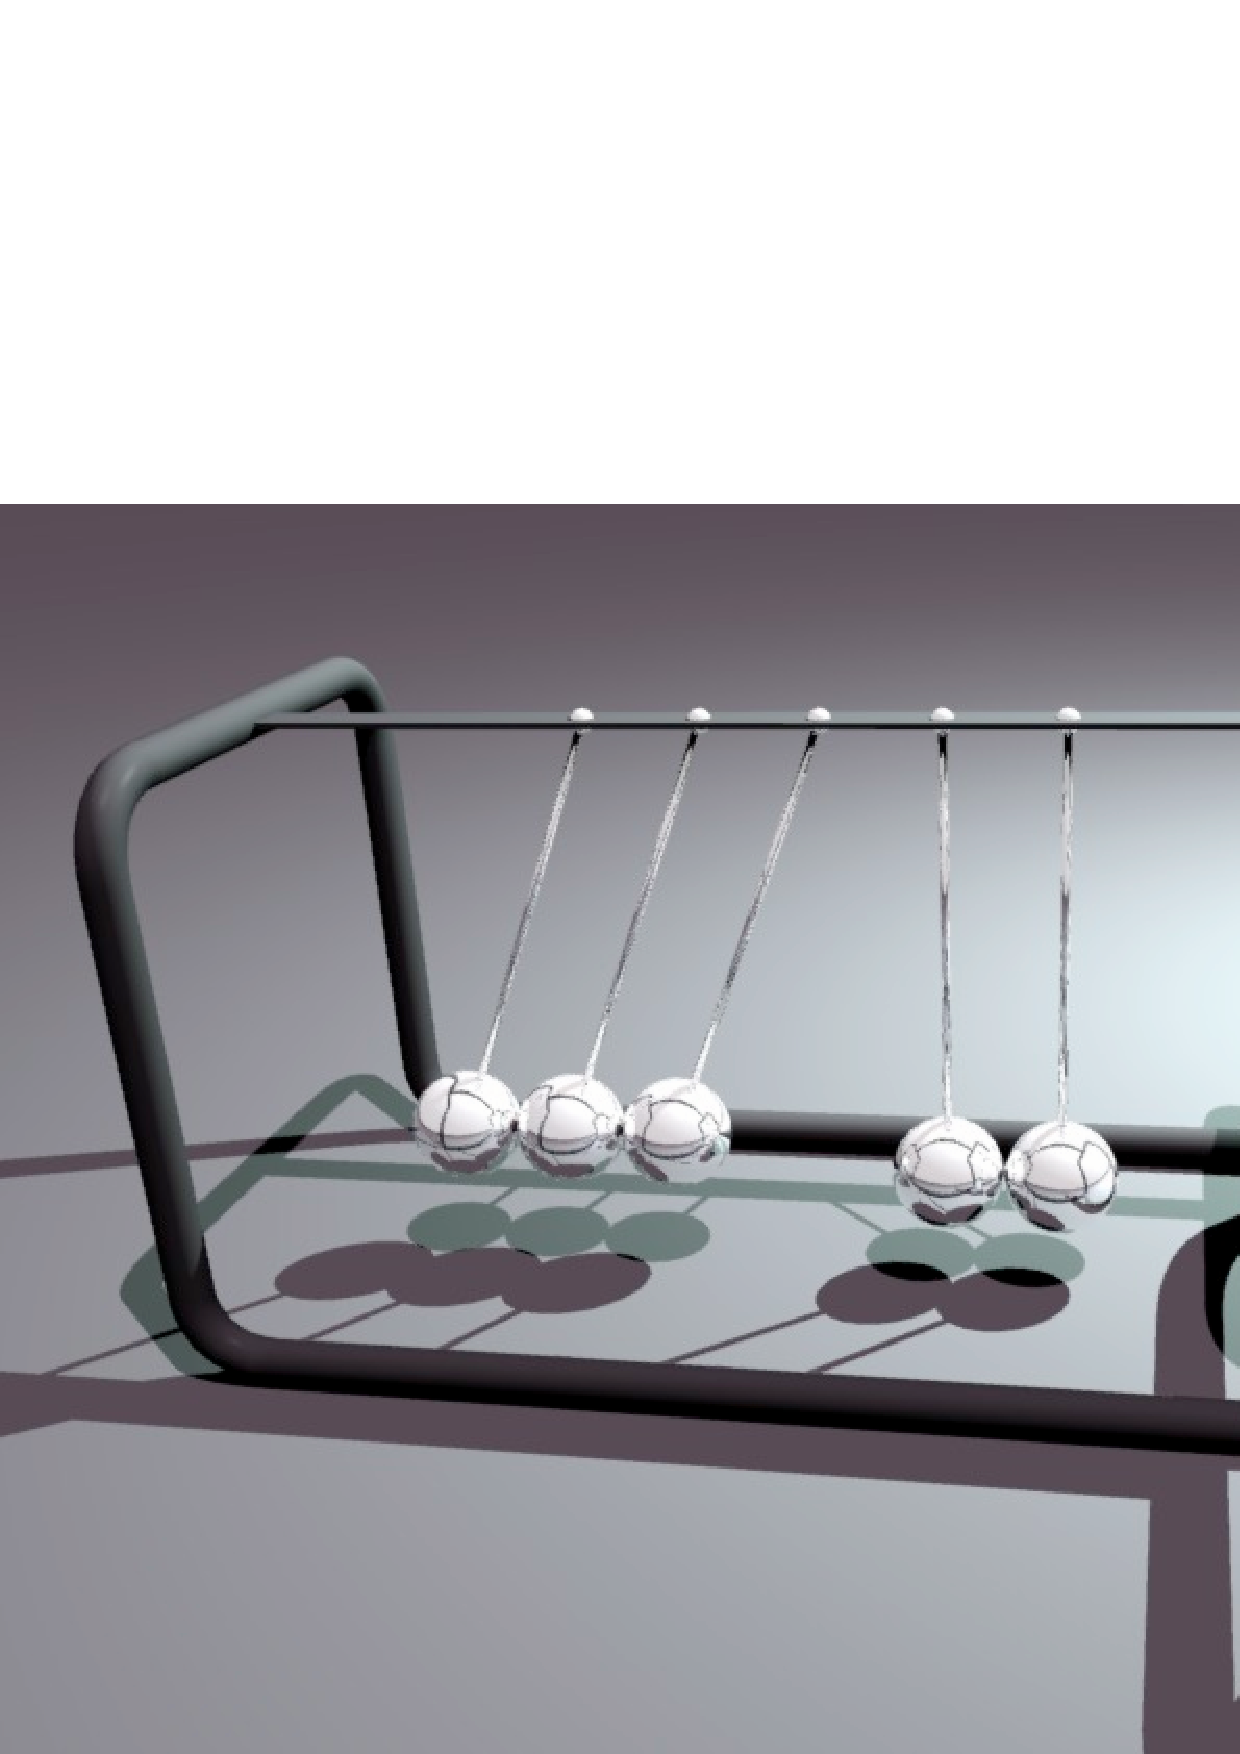
\includegraphics[width=60mm,height=45mm]{figures/cradle1} \hspace{5mm}
            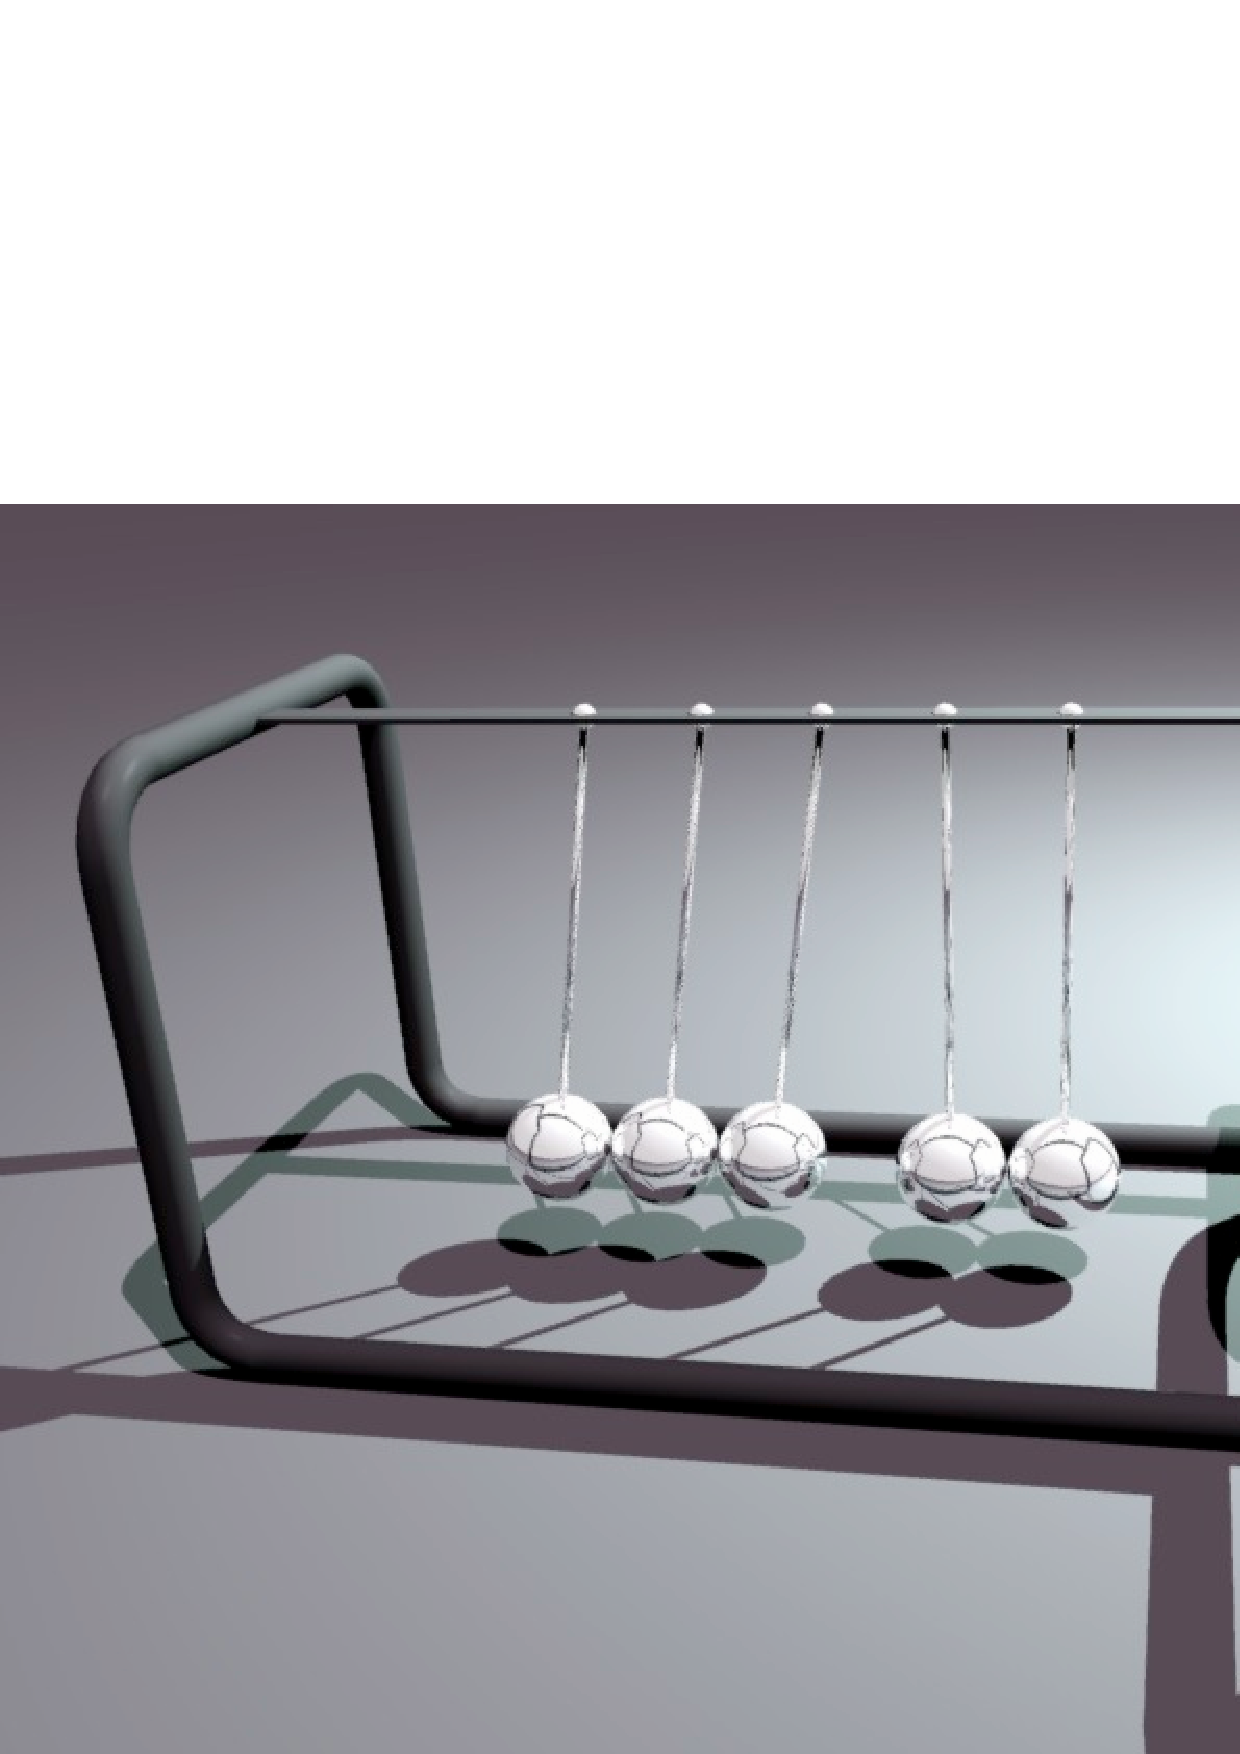
\includegraphics[width=60mm,height=45mm]{figures/cradle2}}\vspace{5mm}
\centerline{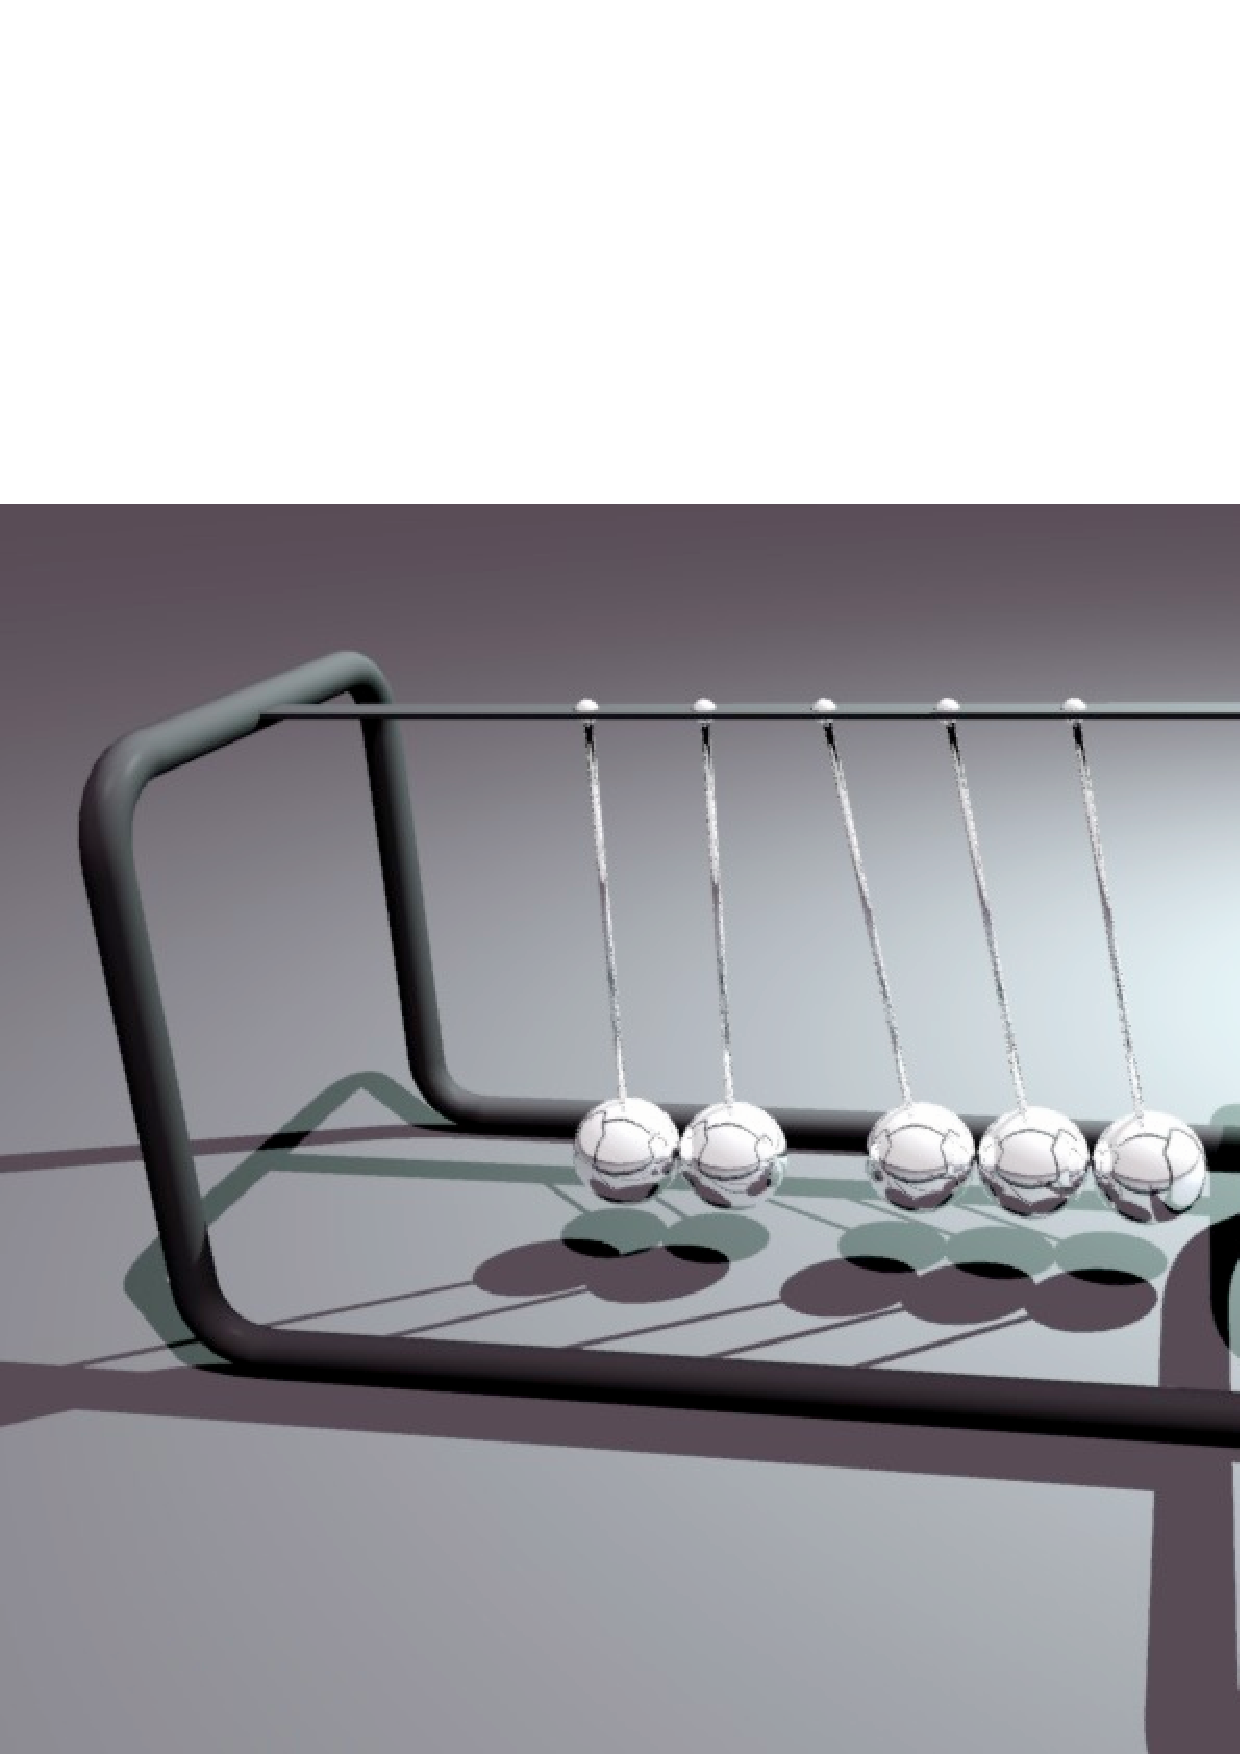
\includegraphics[width=60mm,height=45mm]{figures/cradle3} \hspace{5mm}
            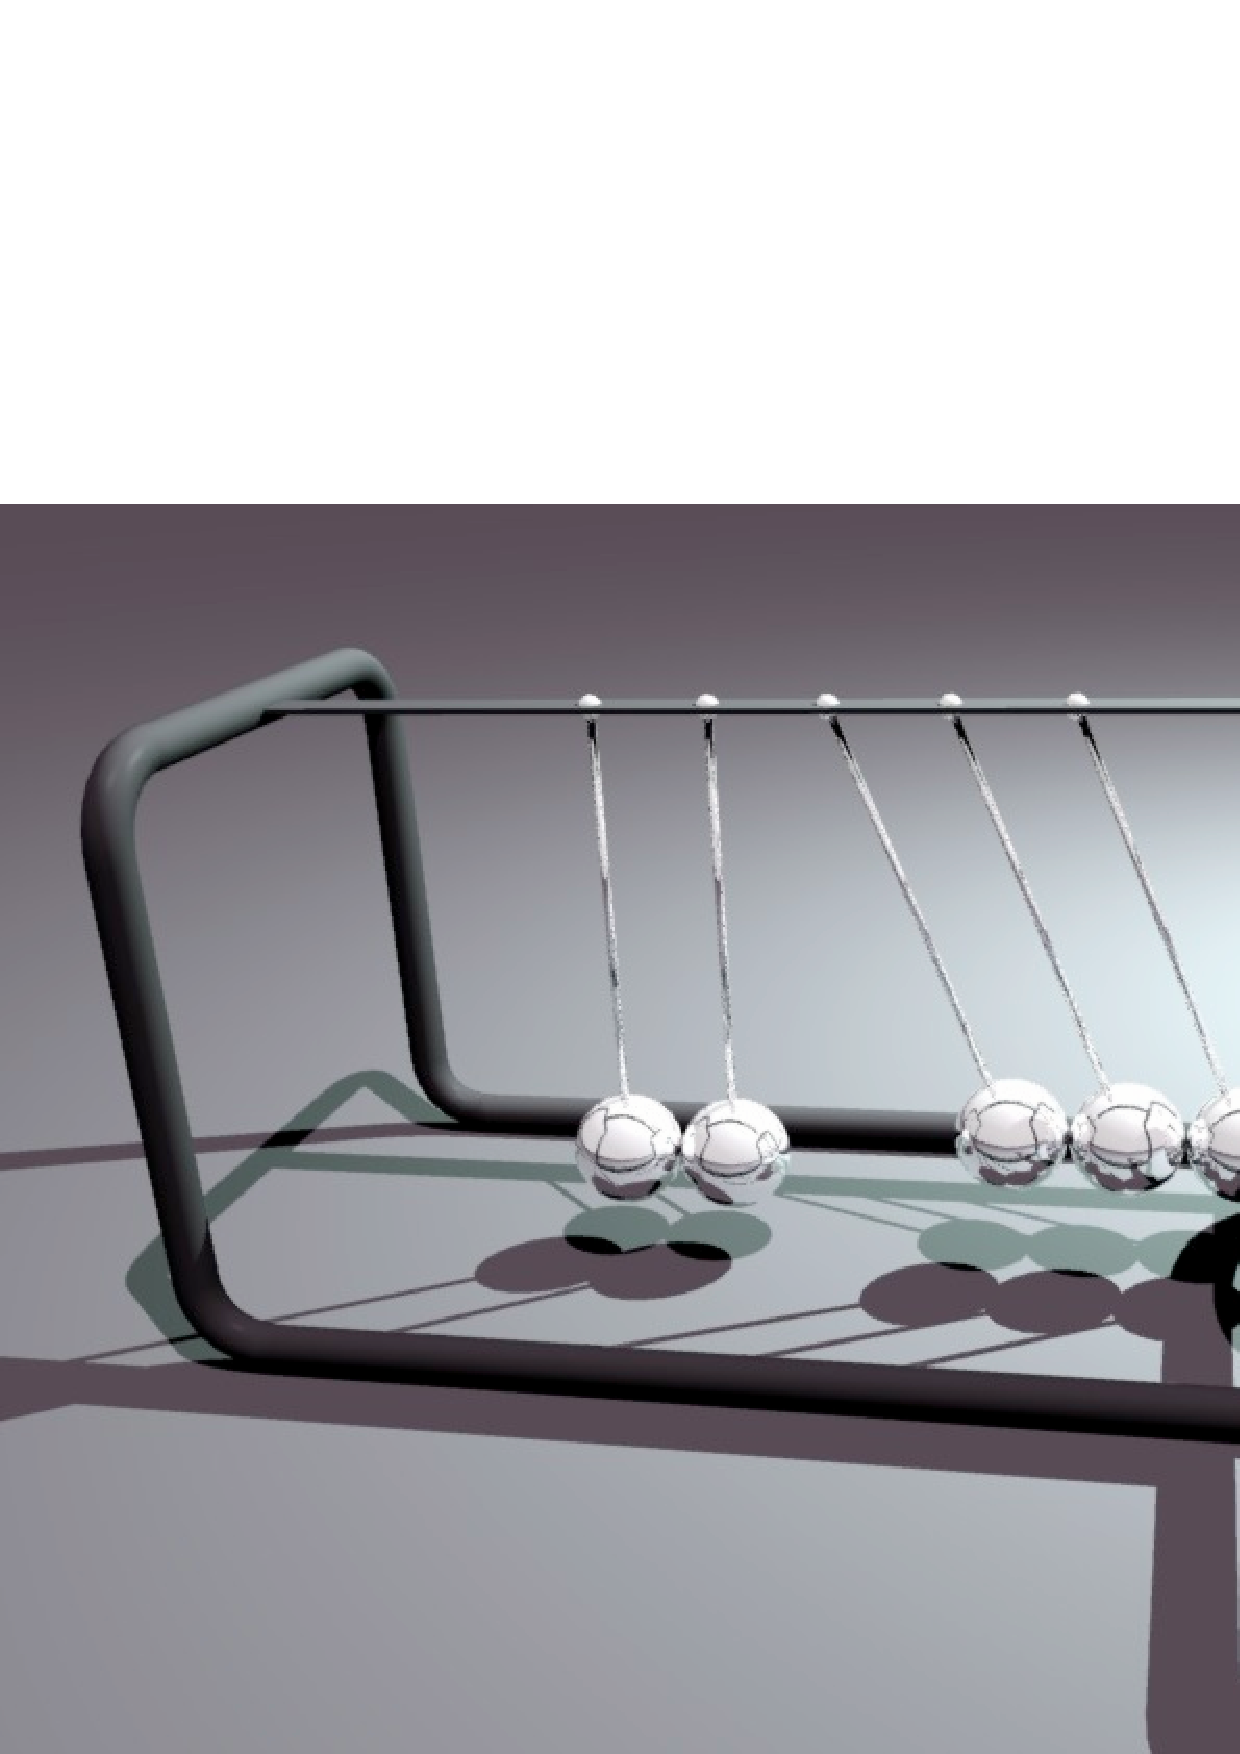
\includegraphics[width=60mm,height=45mm]{figures/cradle4}}
\caption{Animation of Newton's cradle.\label{sampleCradle}}
\end{figure}

\begin{figure}[p]
\centerline{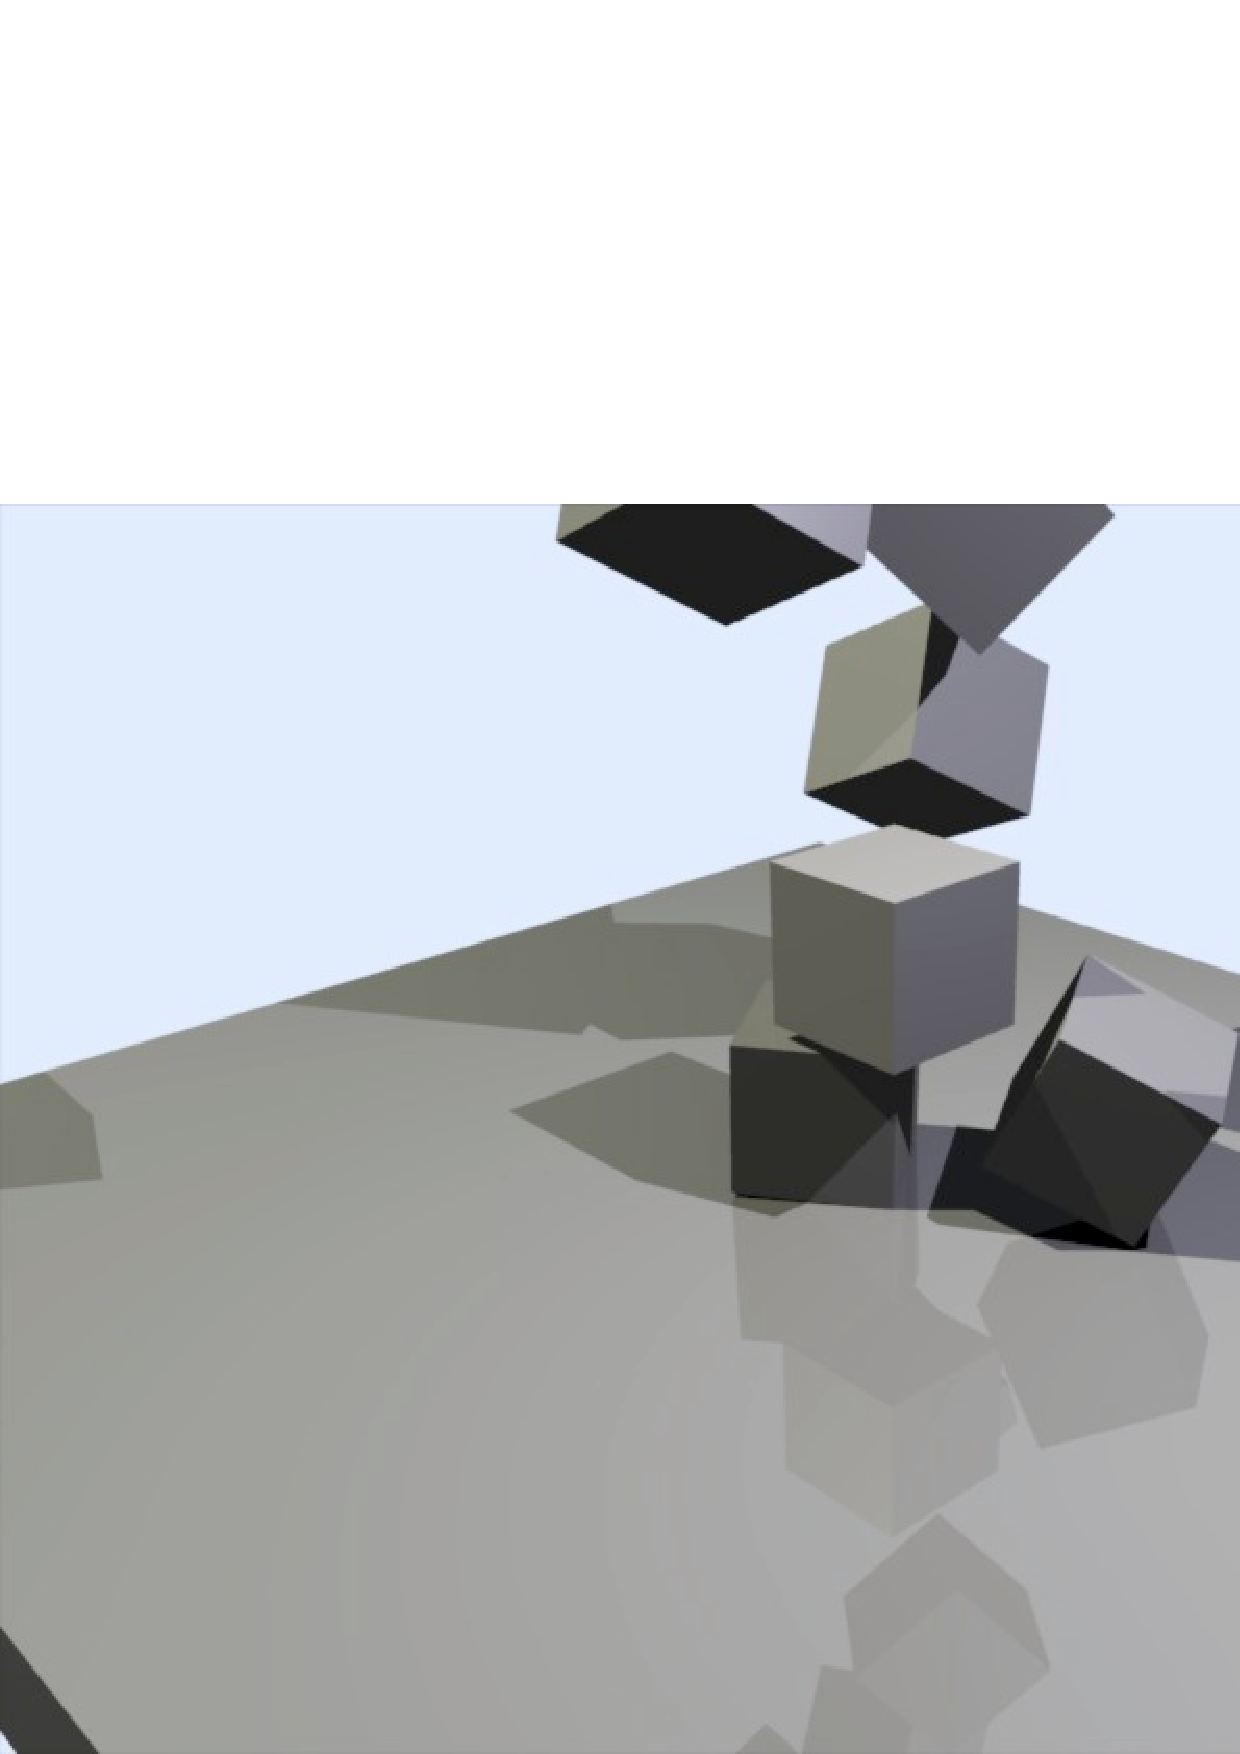
\includegraphics[width=60mm,height=45mm]{figures/boxes1} \hspace{5mm}
            
\includegraphics[width=60mm,height=45mm]{figures/boxes2}}\vspace{5mm}
\centerline{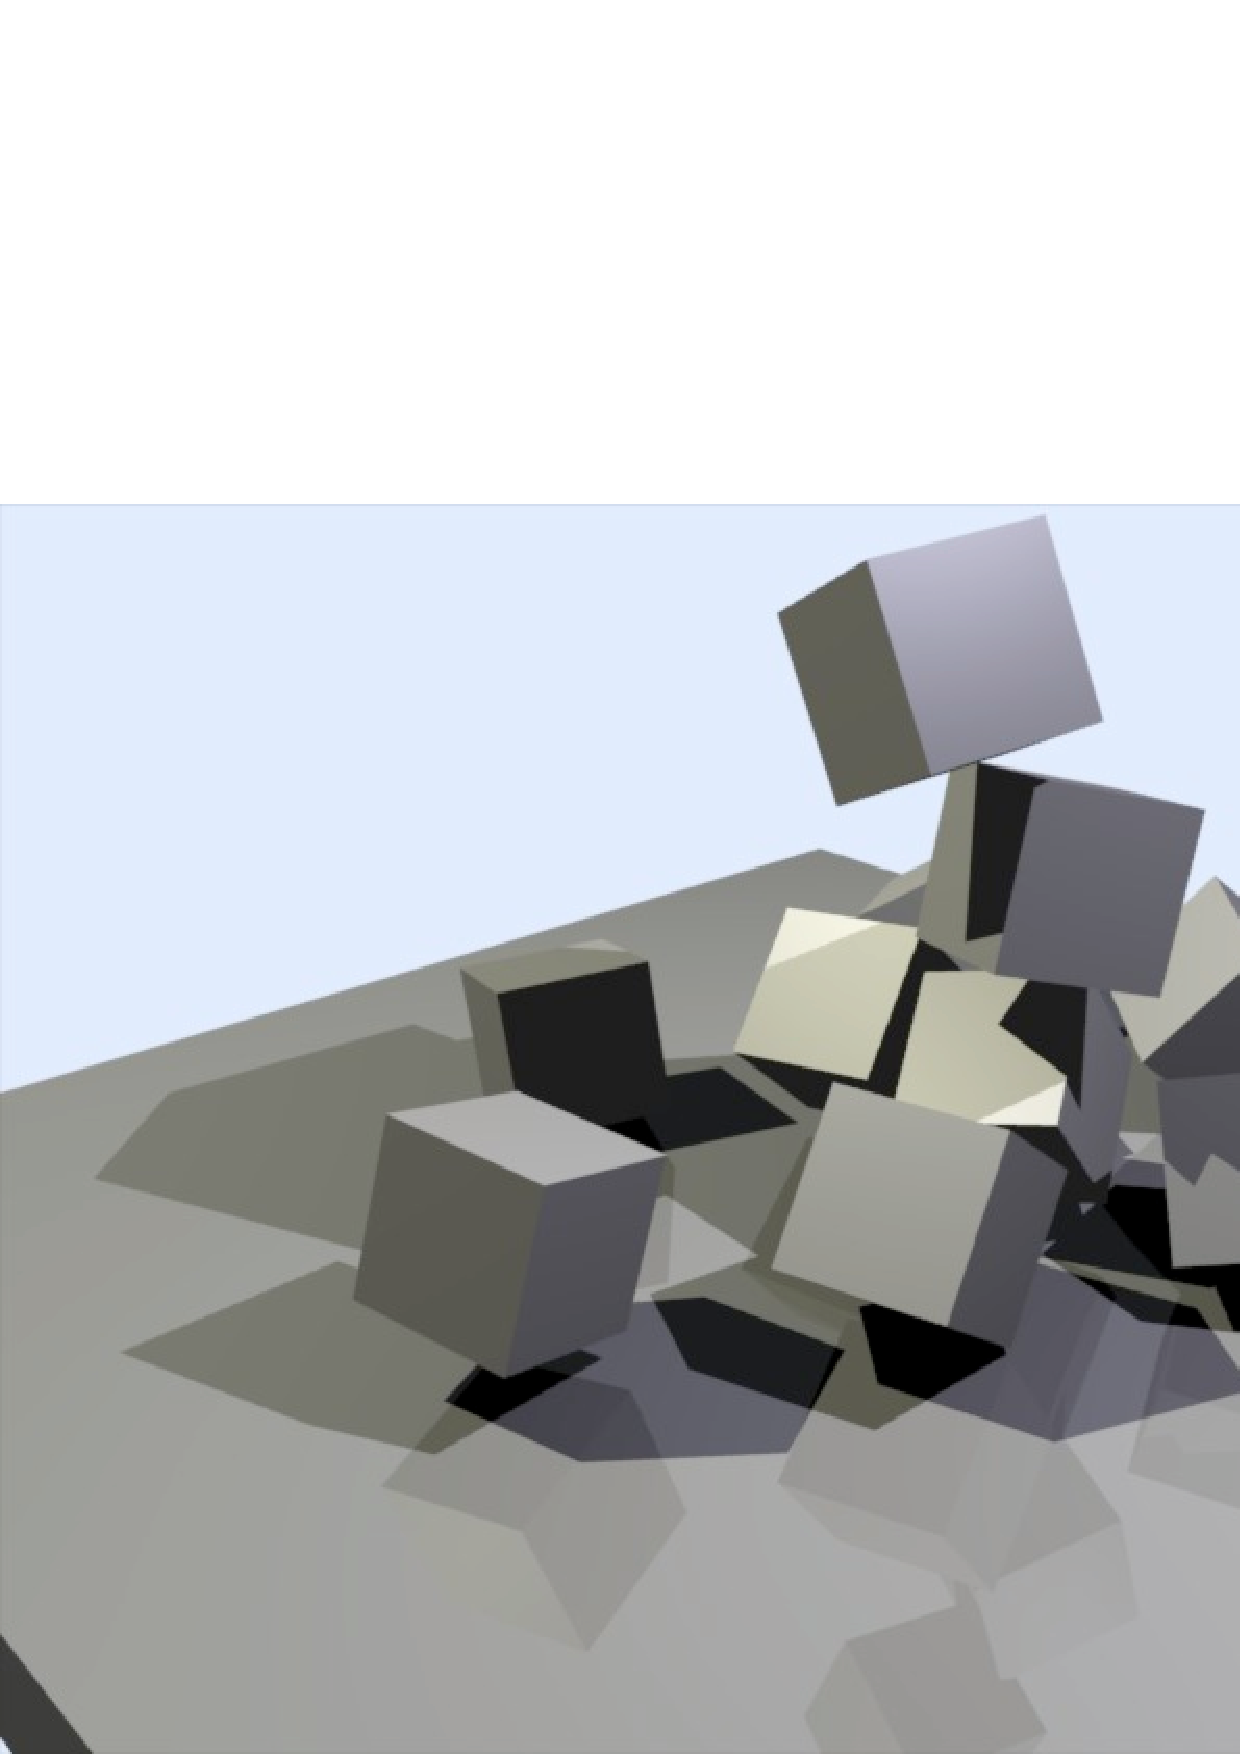
\includegraphics[width=60mm,height=45mm]{figures/boxes3} \hspace{5mm}
            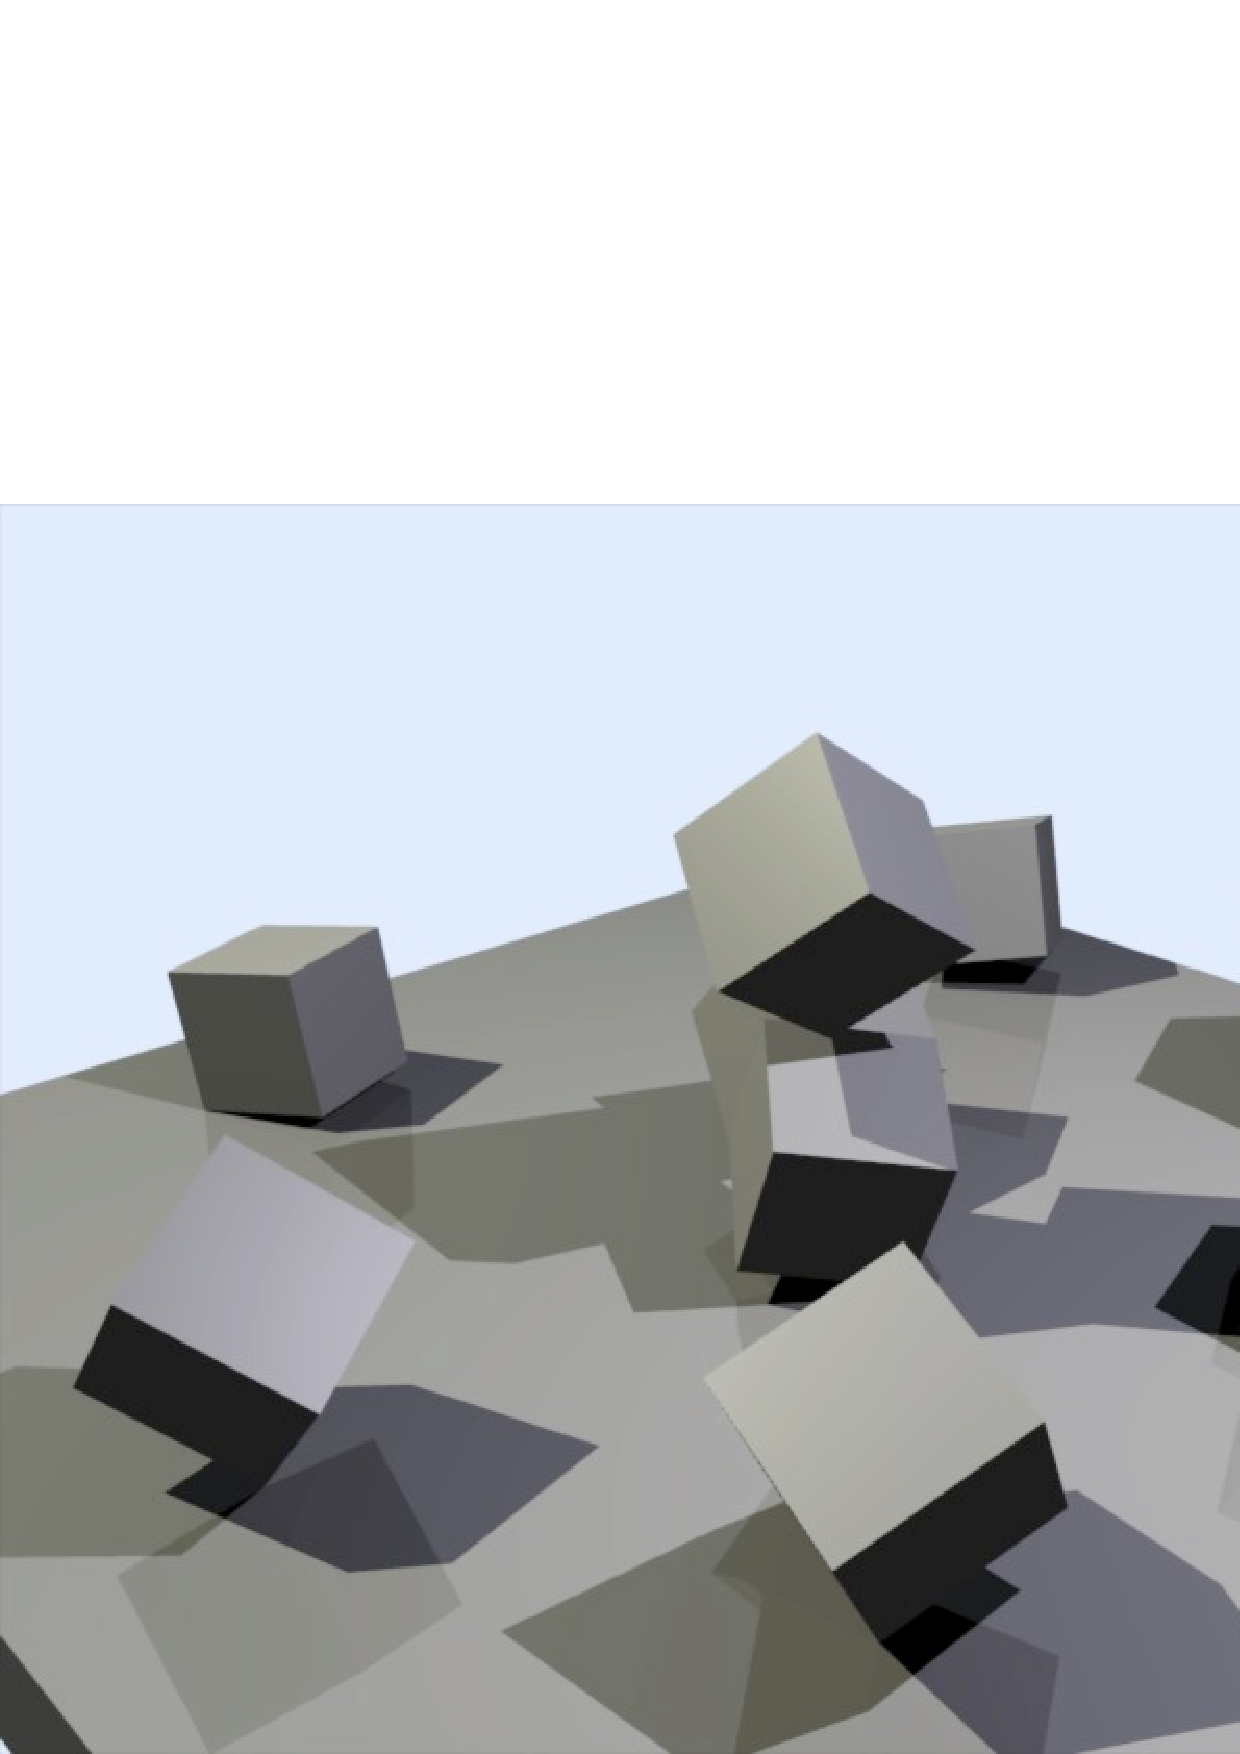
\includegraphics[width=60mm,height=45mm]{figures/boxes4}}
\caption{Animation of ten boxes falling onto a table.\label{sampleBoxes}}
\end{figure}

\begin{figure}[p]
\centerline{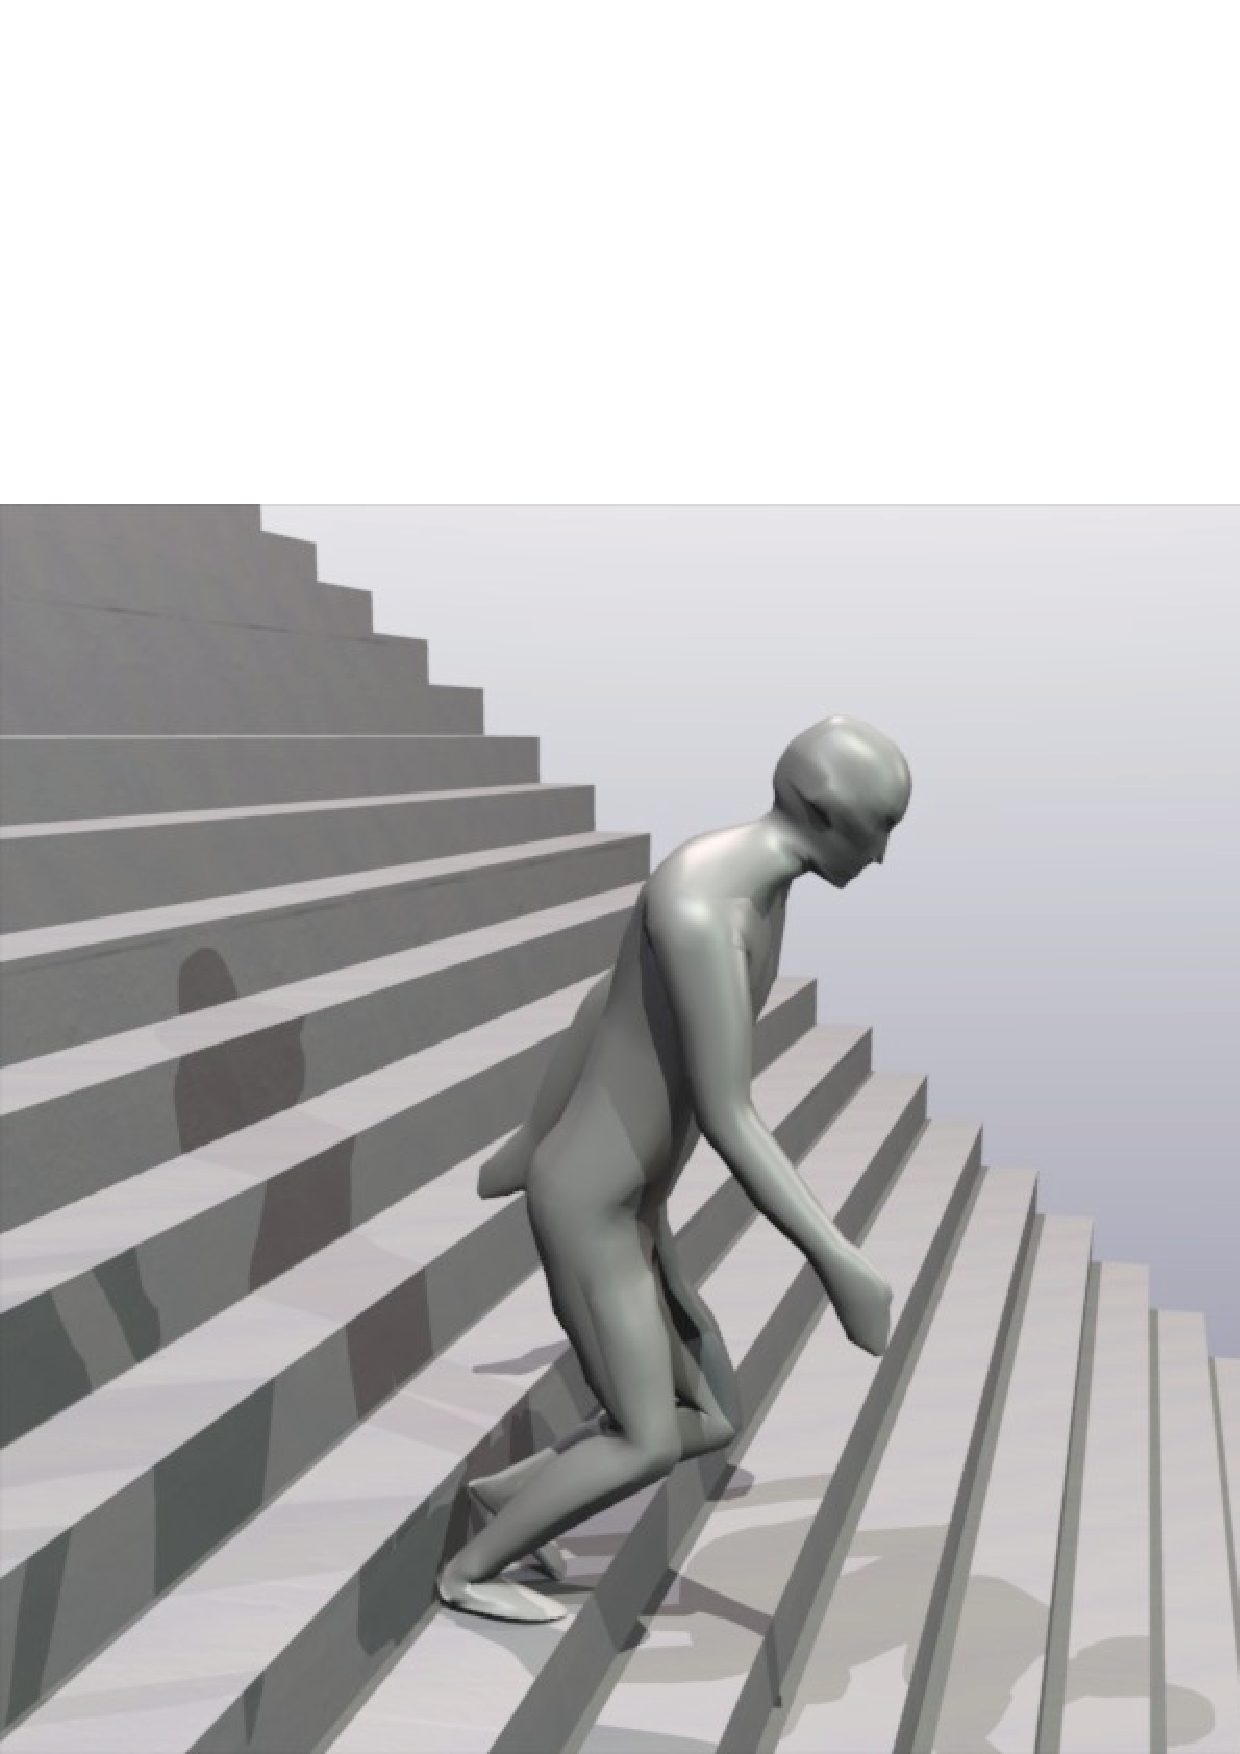
\includegraphics[width=60mm,height=45mm]{figures/stairs1} \hspace{5mm}
            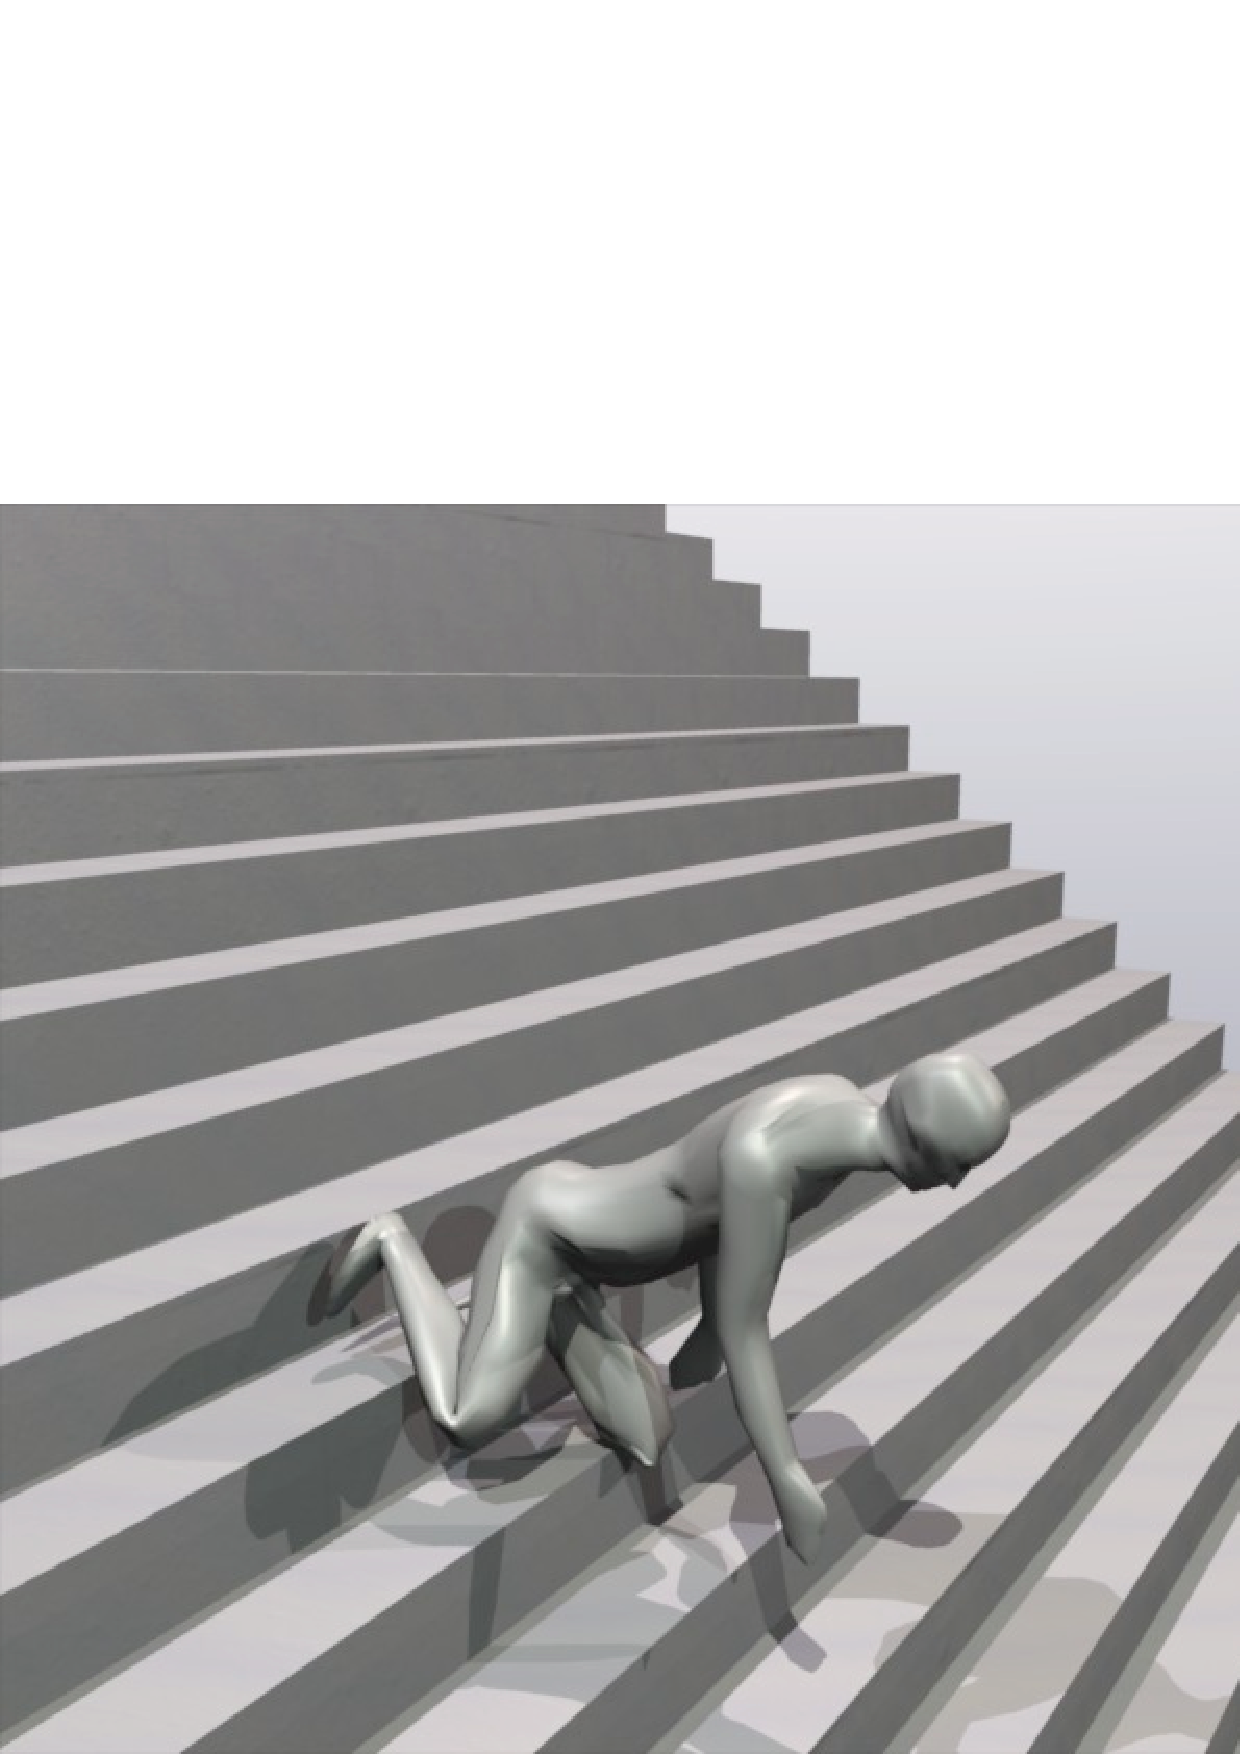
\includegraphics[width=60mm,height=45mm]{figures/stairs2}}\vspace{5mm}
\centerline{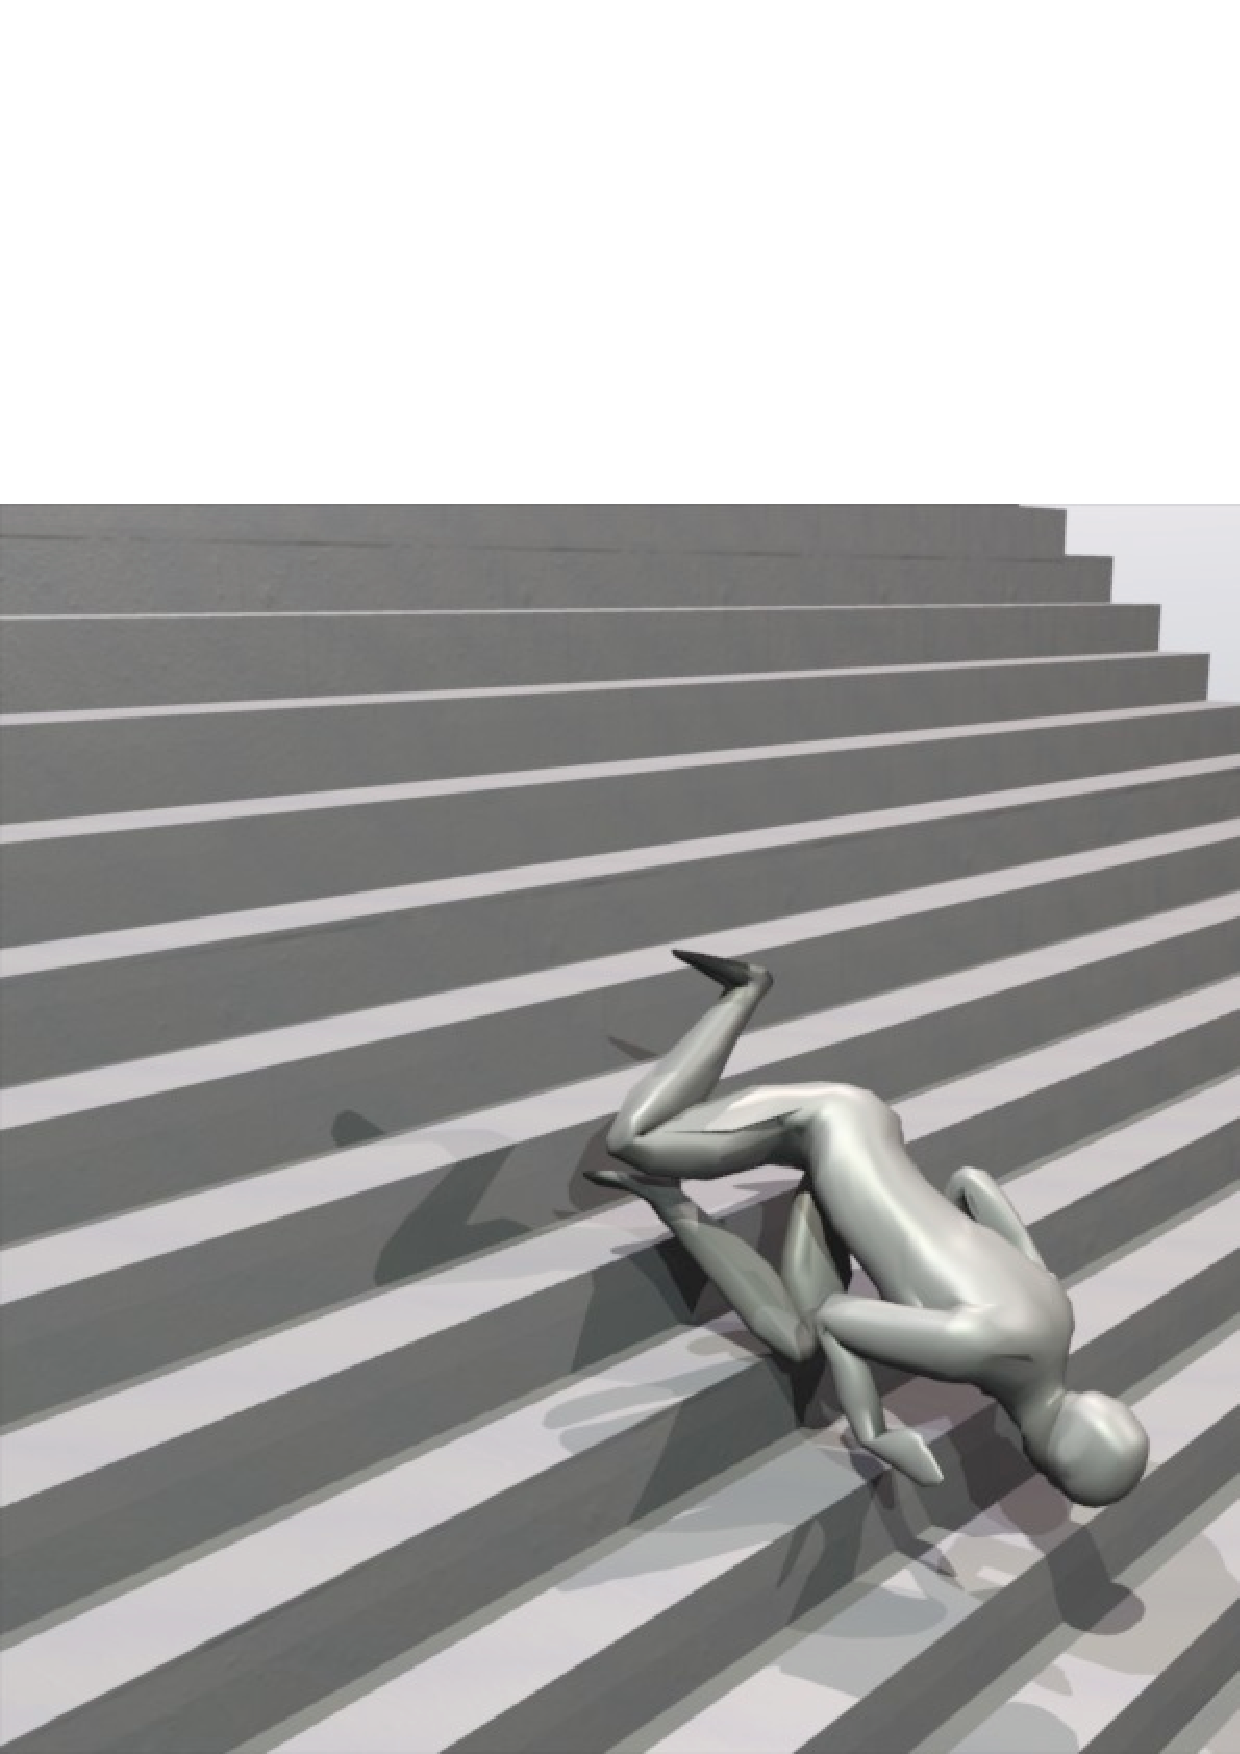
\includegraphics[width=60mm,height=45mm]{figures/stairs3} \hspace{5mm}
            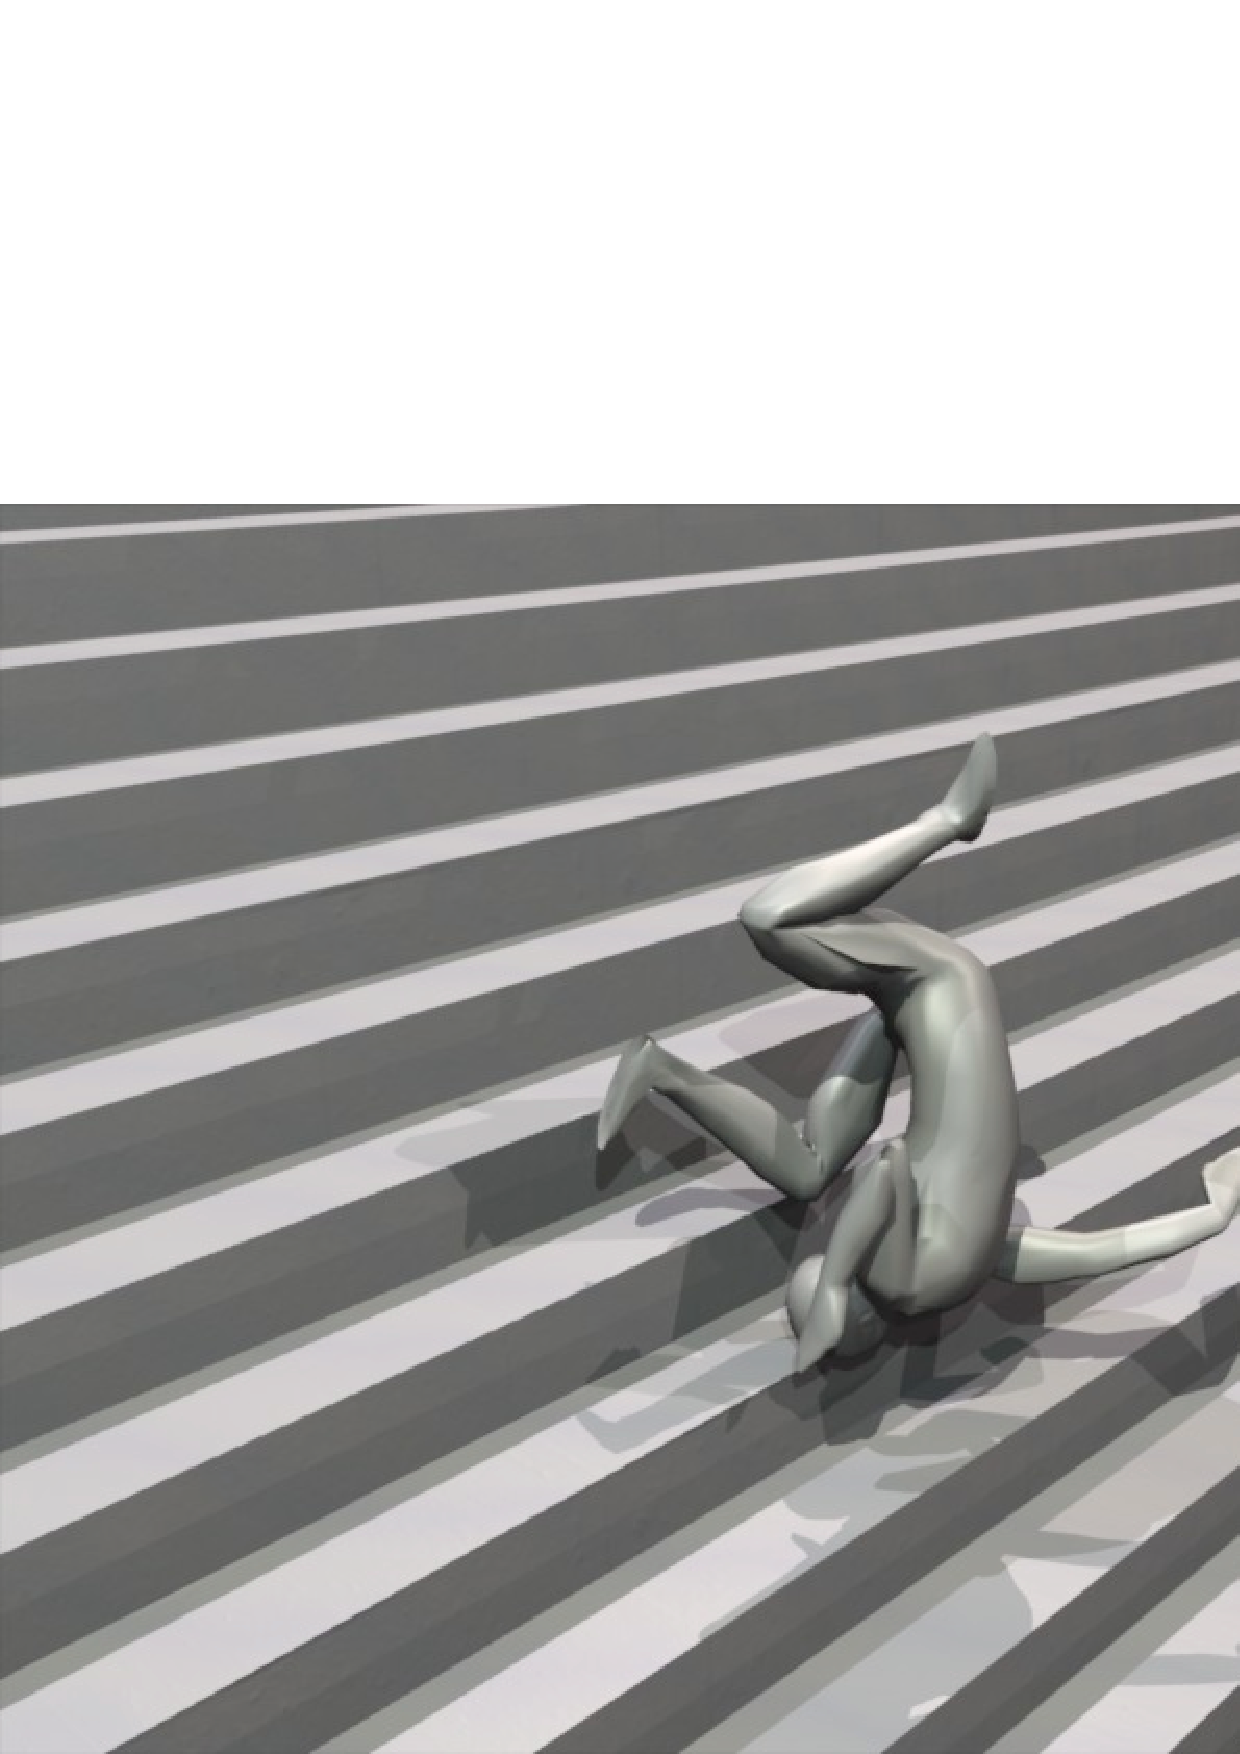
\includegraphics[width=60mm,height=45mm]{figures/stairs4}}
\caption{Animation of Alfred falling down a set of stairs.\label{sampleStairs}}
\end{figure}

\begin{figure}[p]
\centerline{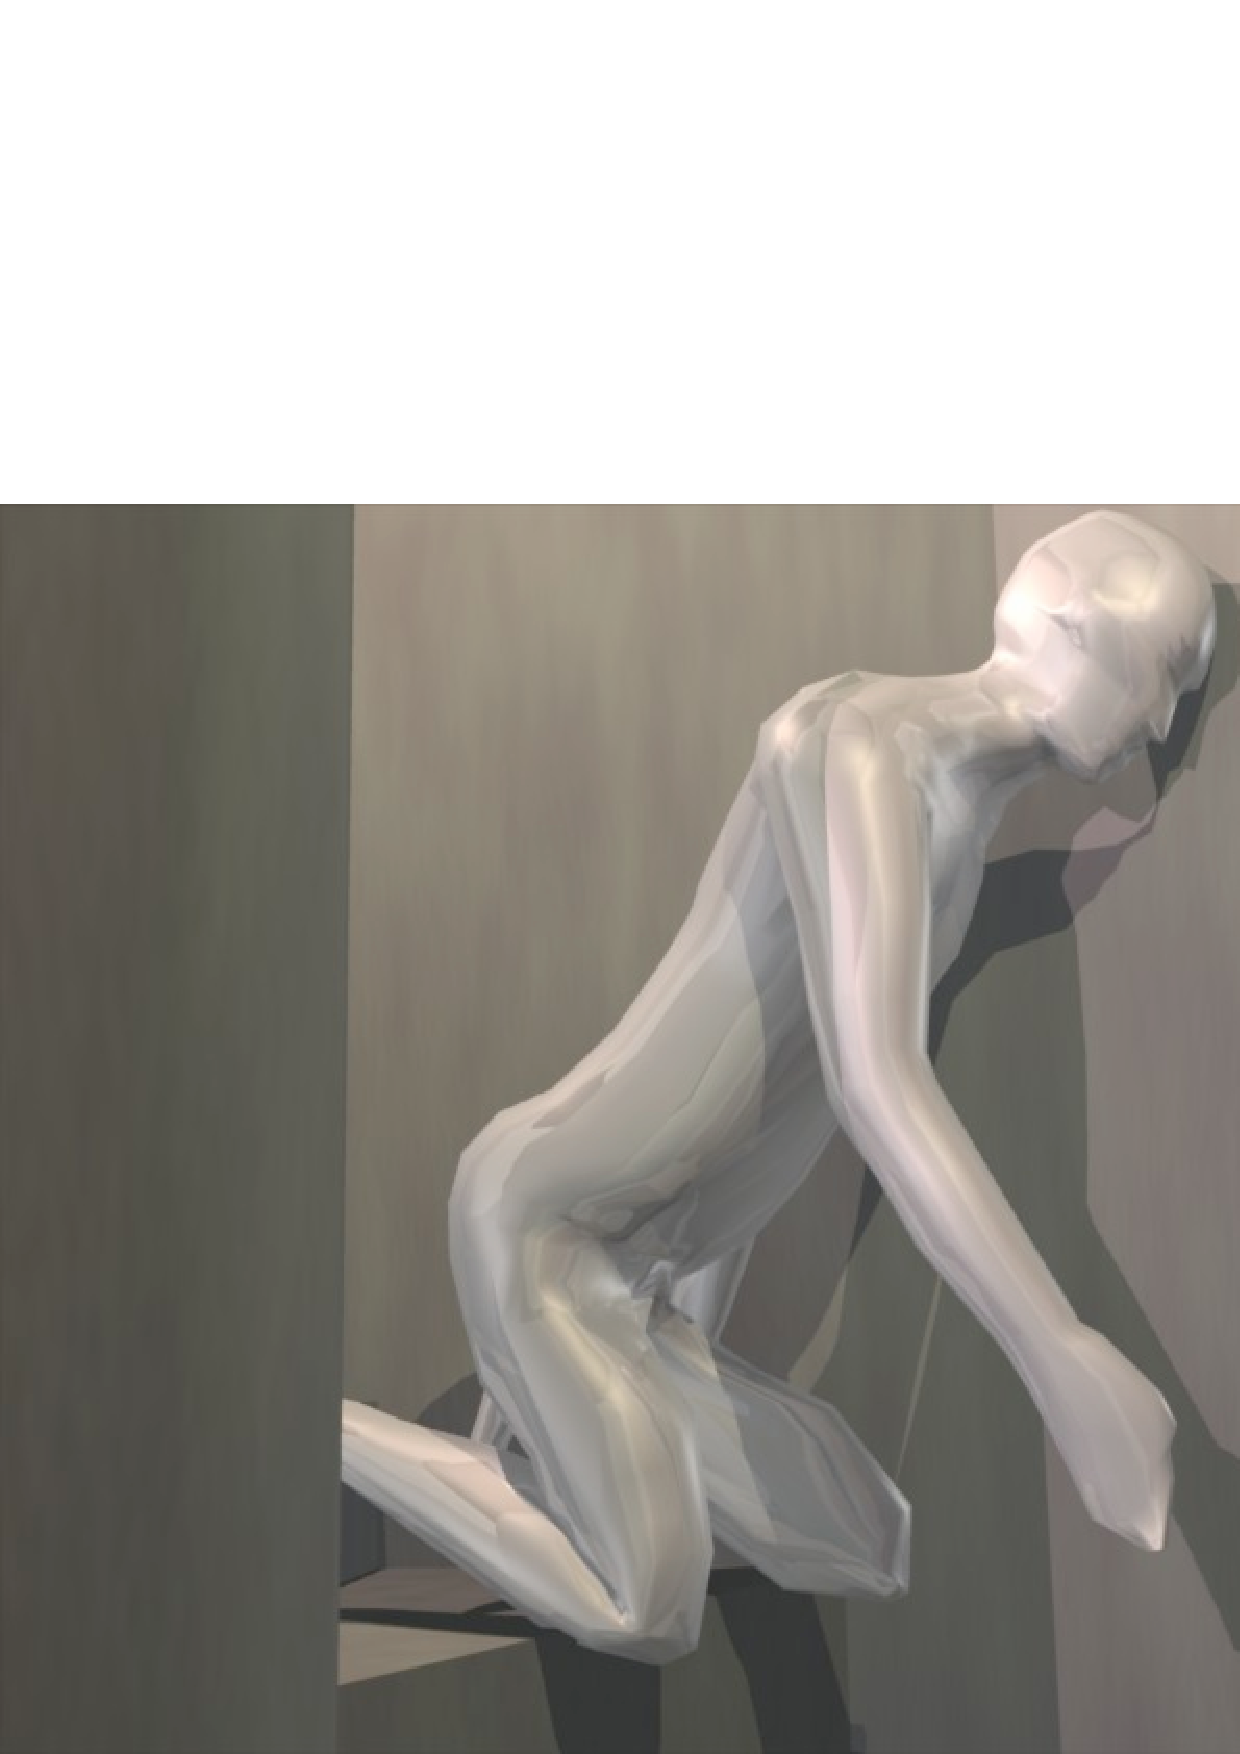
\includegraphics[width=60mm,height=45mm]{figures/spiral1} \hspace{5mm}
            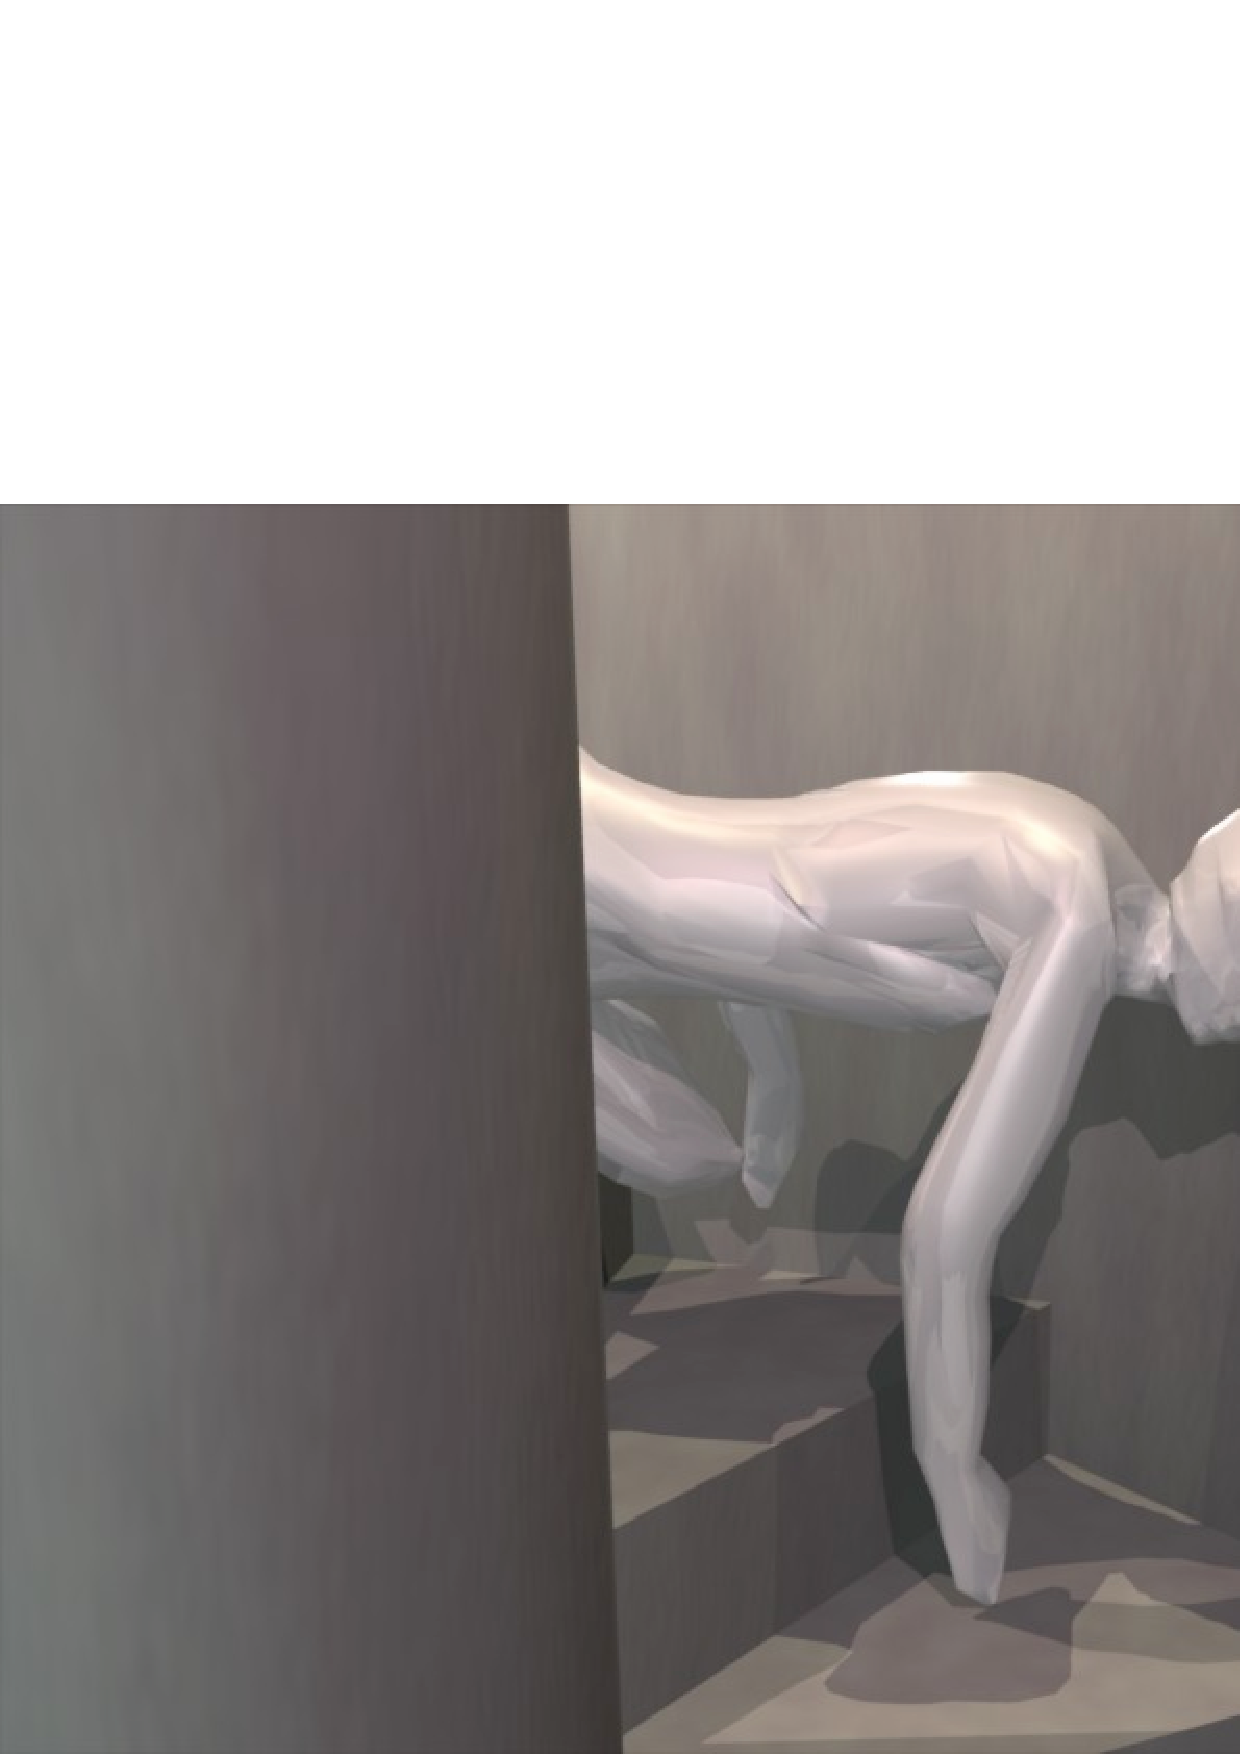
\includegraphics[width=60mm,height=45mm]{figures/spiral2}}\vspace{5mm}
\centerline{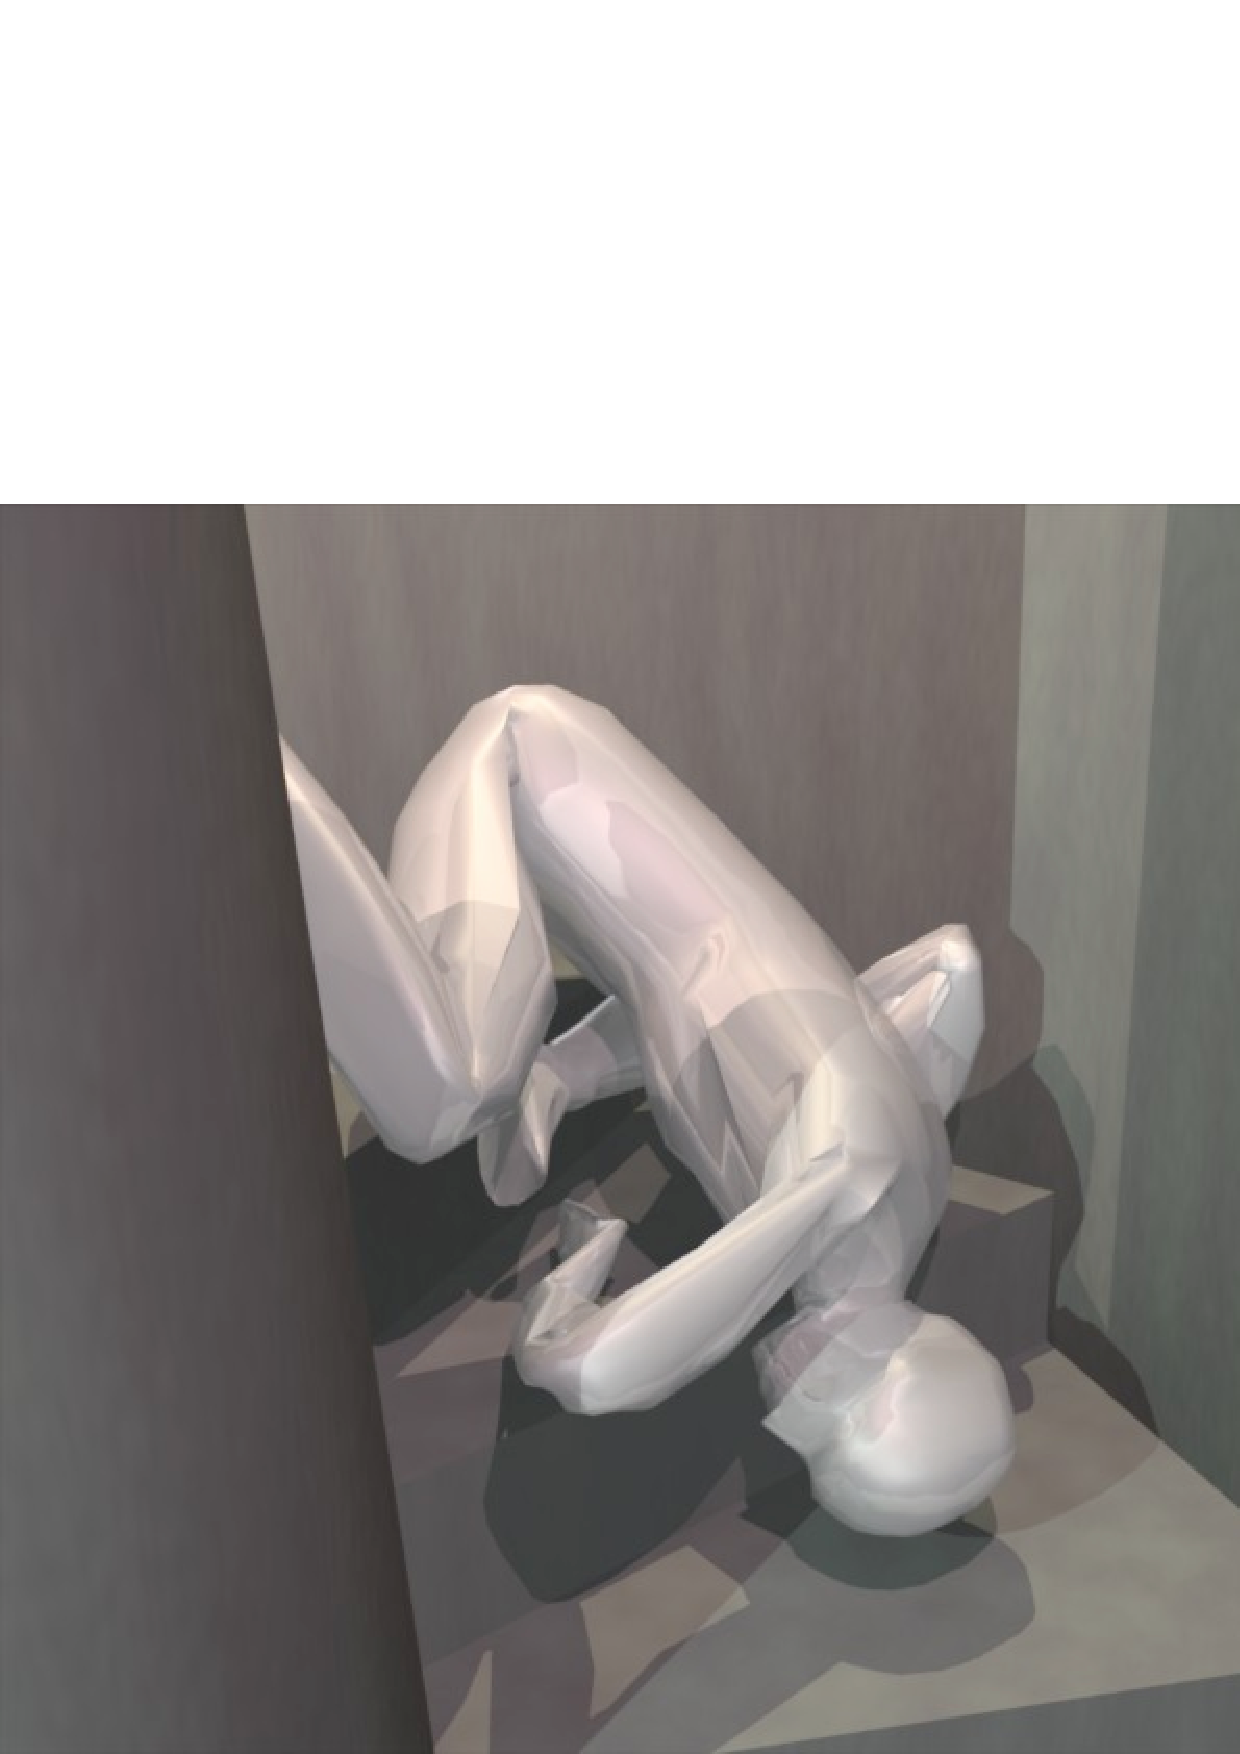
\includegraphics[width=60mm,height=45mm]{figures/spiral3} \hspace{5mm}
            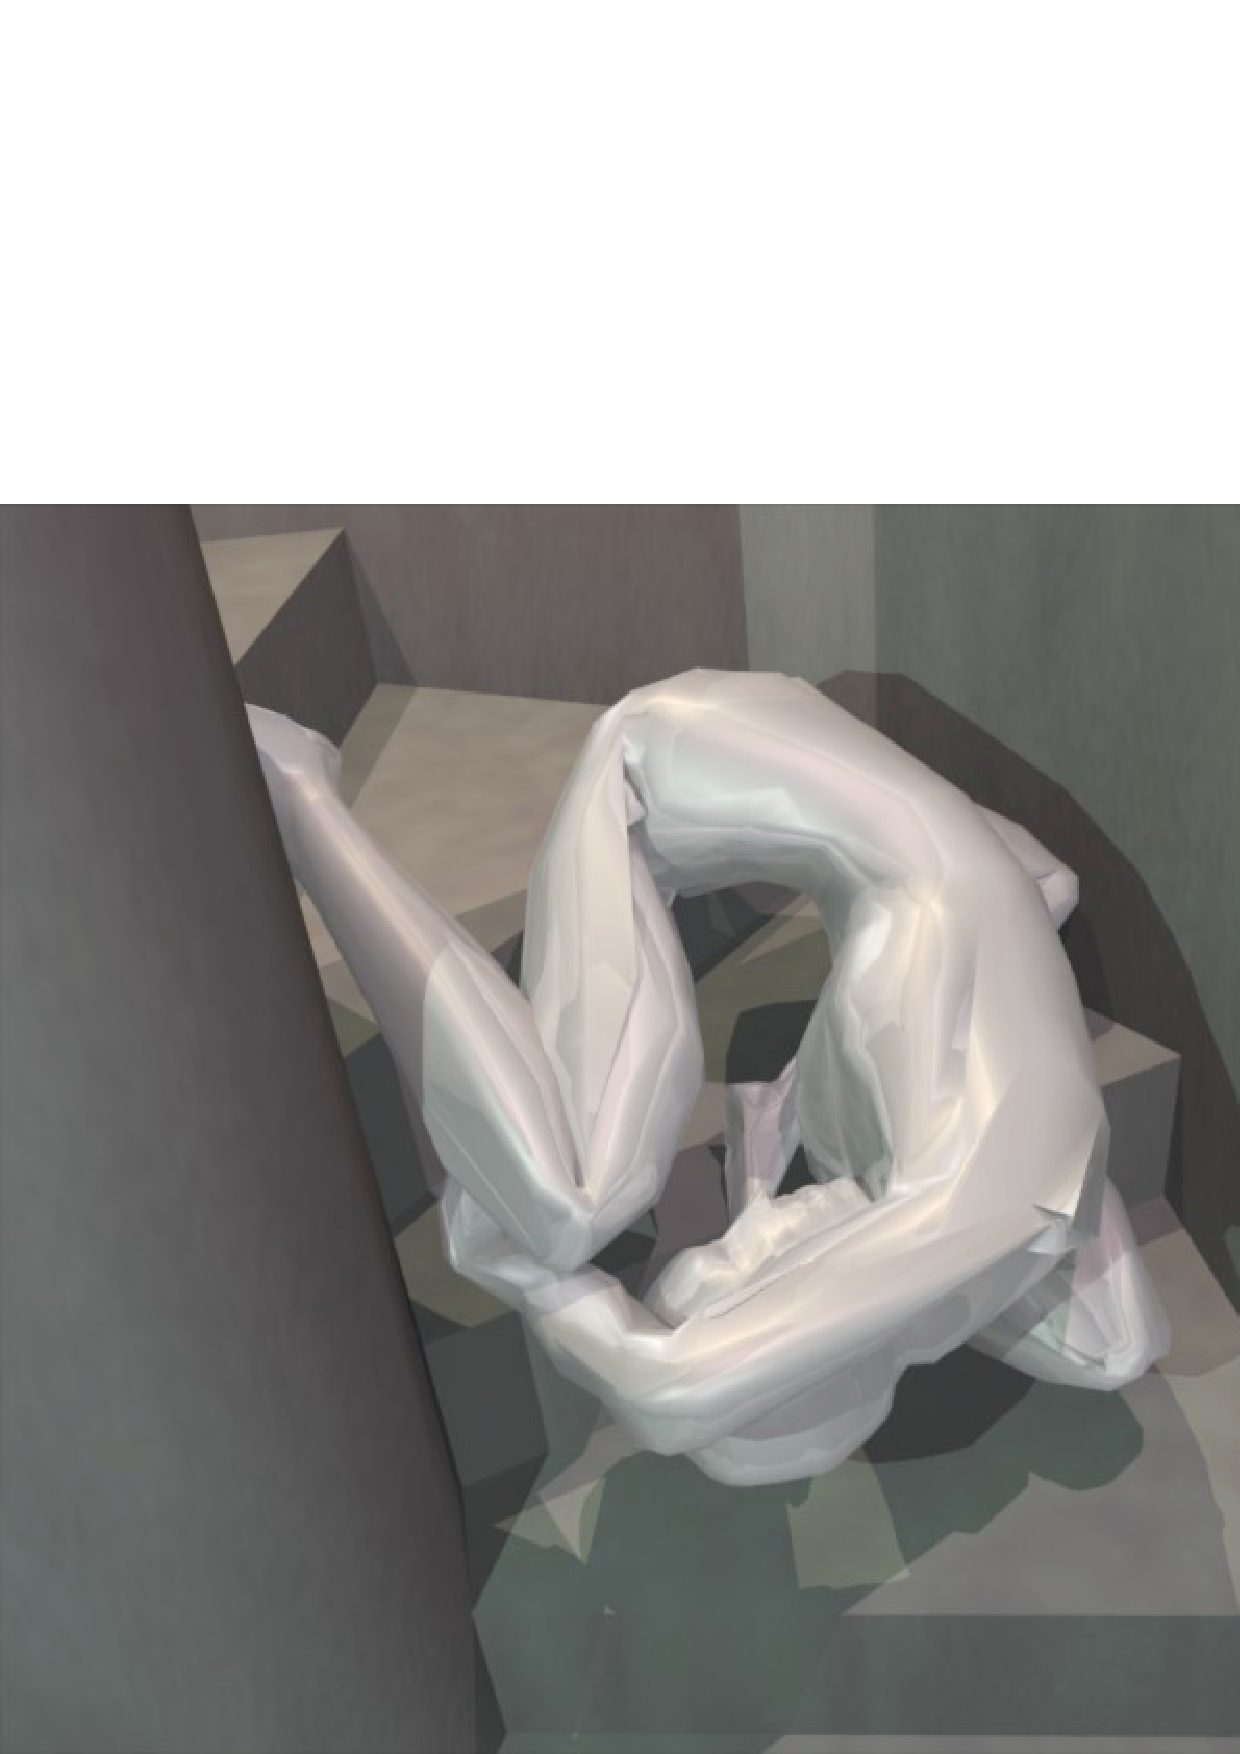
\includegraphics[width=60mm,height=45mm]{figures/spiral4}}
\caption{Animation of Alfred tumbling down a spiral staircase.\label{sampleSpiral}}
\end{figure}

\section{Simulation examples}

In the end, the purpose of this project is to produce animations for computer graphics, and the
last word must be given to the human observer who watches these animations. I would like to claim
that the results are of a quality similar to what an animator might create, and that they are
realistic in the sense that they do not violate the laws of physics or anatomy. However, such a
claim is difficult to defend convincingly in print. I have therefore compiled a video of several
example animations, and I urge the reader to watch it to gain a more personal impression of this
project's results. The video can be found in the 3D graphics section of my web site
\texttt{http://martin.kleppmann.de/}. The following sections describe how each of the simulated
systems was implemented and point out noteworthy features.

\subsection{Pendulum systems}

The simplest physical system in the demonstration video is
the animation of a double pendulum (a rigid pendulum with a second one
attached to its end), and its extension to three, eight and 25 segments. The double pendulum is
a commonly studied system in physics; although it does not have an exact analytic solution, an
approximate solution can be found for small angles. In this case, one finds that the resulting
movement is the sum of two simple harmonic oscillations at different frequencies, resulting in
a mysterious-looking swinging movement.

The double, triple and eight-part pendulums are set up in a very similar way. Each segment is
modelled as a rigid cylinder with constant density. The top end of the top segment is held in
place by a `nail' constraint. Each pair of adjacent segments is connected by a ball-and-socket
joint. Initially, all segments are at rest, the first segment is rotated by 45 degrees
anticlockwise from the equilibrium position, and all other segments hang straight down.

The simulation does not employ an XML input file; instead, the objects representing the bodies
and the constraints are directly created by the Java test case. The simulation results were
exported to Blender and rendered using the internal renderer and orthographic projection.
I also performed a Fourier transform on the results of the double pendulum simulation, which
indicated very clearly that there were two main frequency components.

The 25-segment pendulum is an attempt to simulate rope, and it is considerably more ambitious.
It is modelled as a cylindrical mesh bound to a chain of 25 bones. The ground is a separate mesh,
and in the simulation its position is fixed by three `nail' constraints. This input data is
represented as an XML file. Collision detection is performed on basis of the meshes, thus the
rope can collide both with itself and with the ground.

The joints between adjacent segments of the rope are of ball-and-socket type, and their rotation
is limited to a maximum of 15 degrees about each axis. The si\-mu\-la\-ted rope is therefore very
stiff. I am not entirely sure how realistic I should consider this simulation; its behaviour looks
strange at first, but this is mainly due to the assumptions put into the model. I believe that
the simulation correctly obeys the model, but the model would have to be refined in order
to produce genuinely realistic-looking rope.

\subsection{Newton's cradle}

\begin{figure}[p]
\centerline{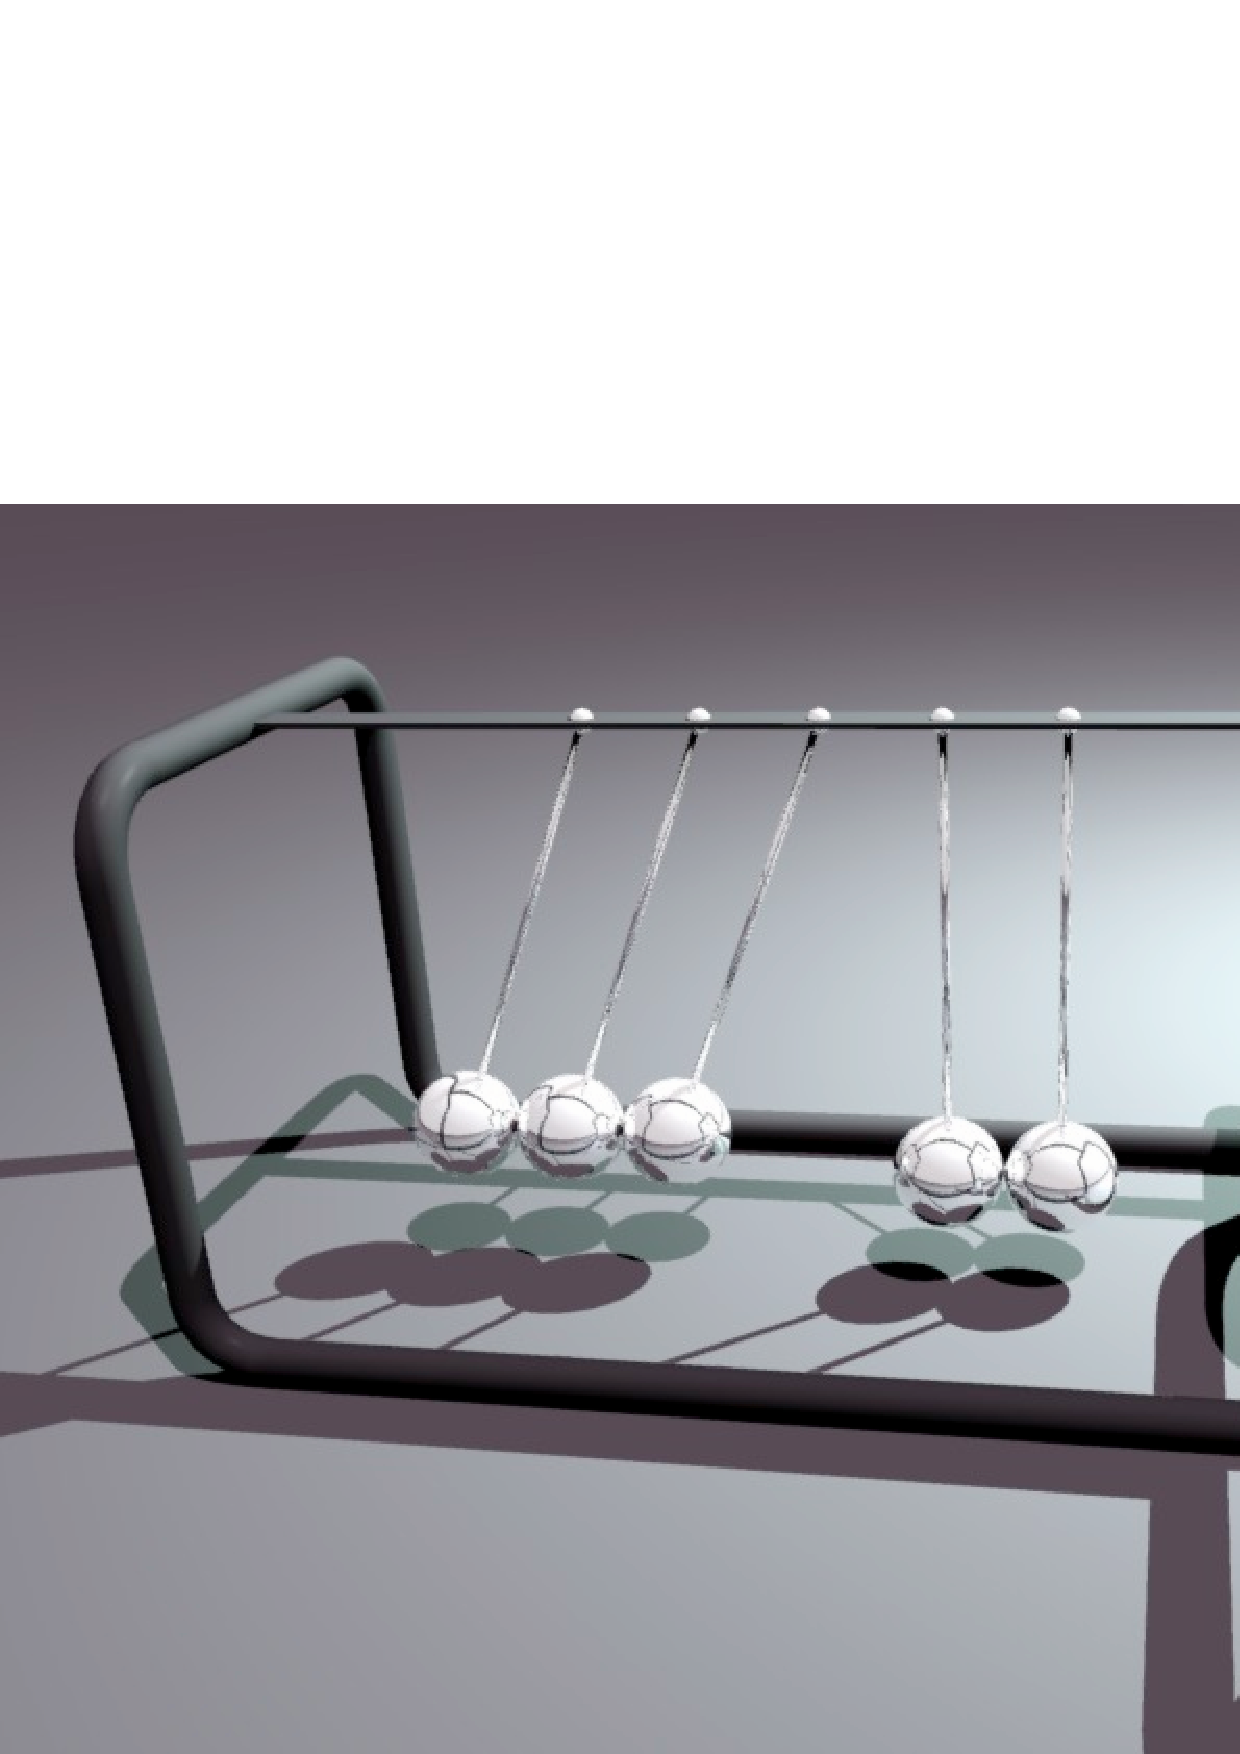
\includegraphics[width=60mm,height=45mm]{figures/cradle1} \hspace{5mm}
            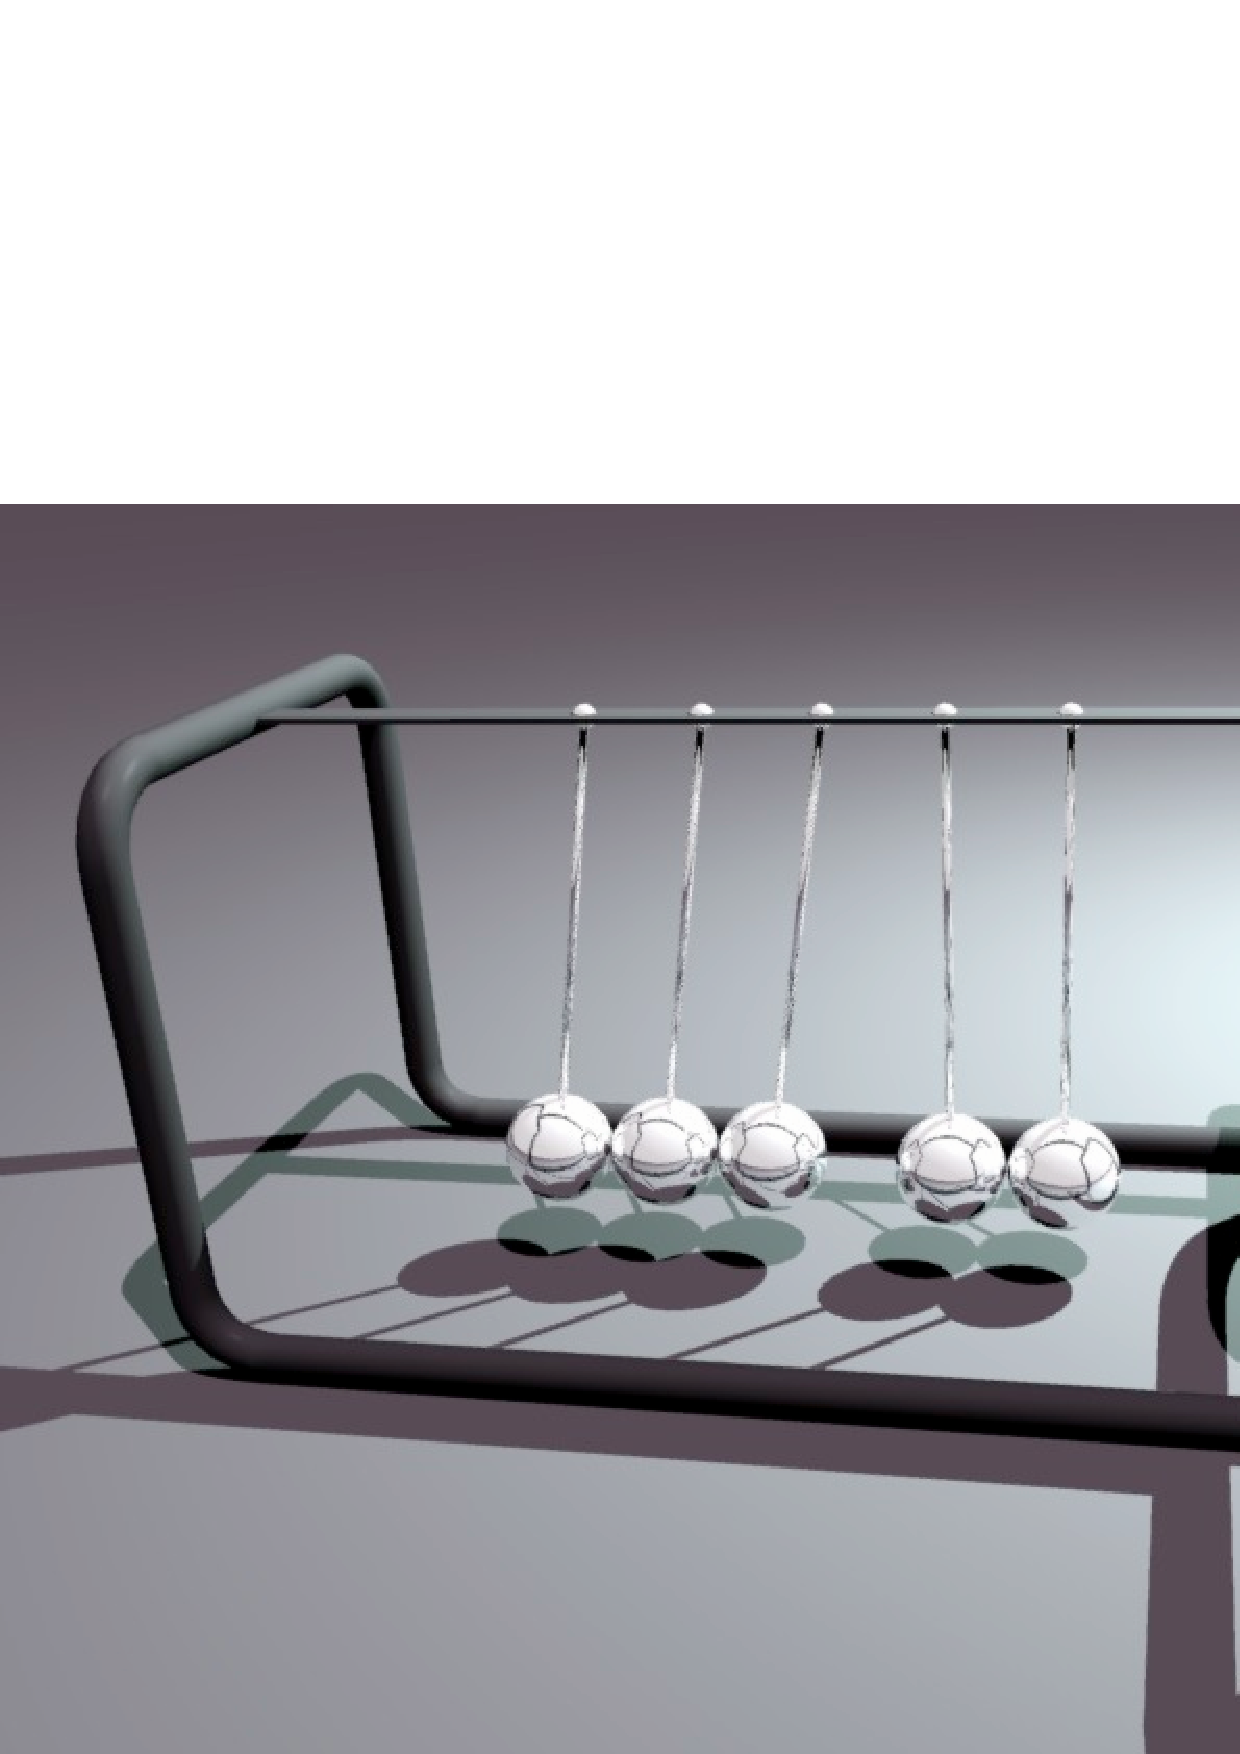
\includegraphics[width=60mm,height=45mm]{figures/cradle2}}\vspace{5mm}
\centerline{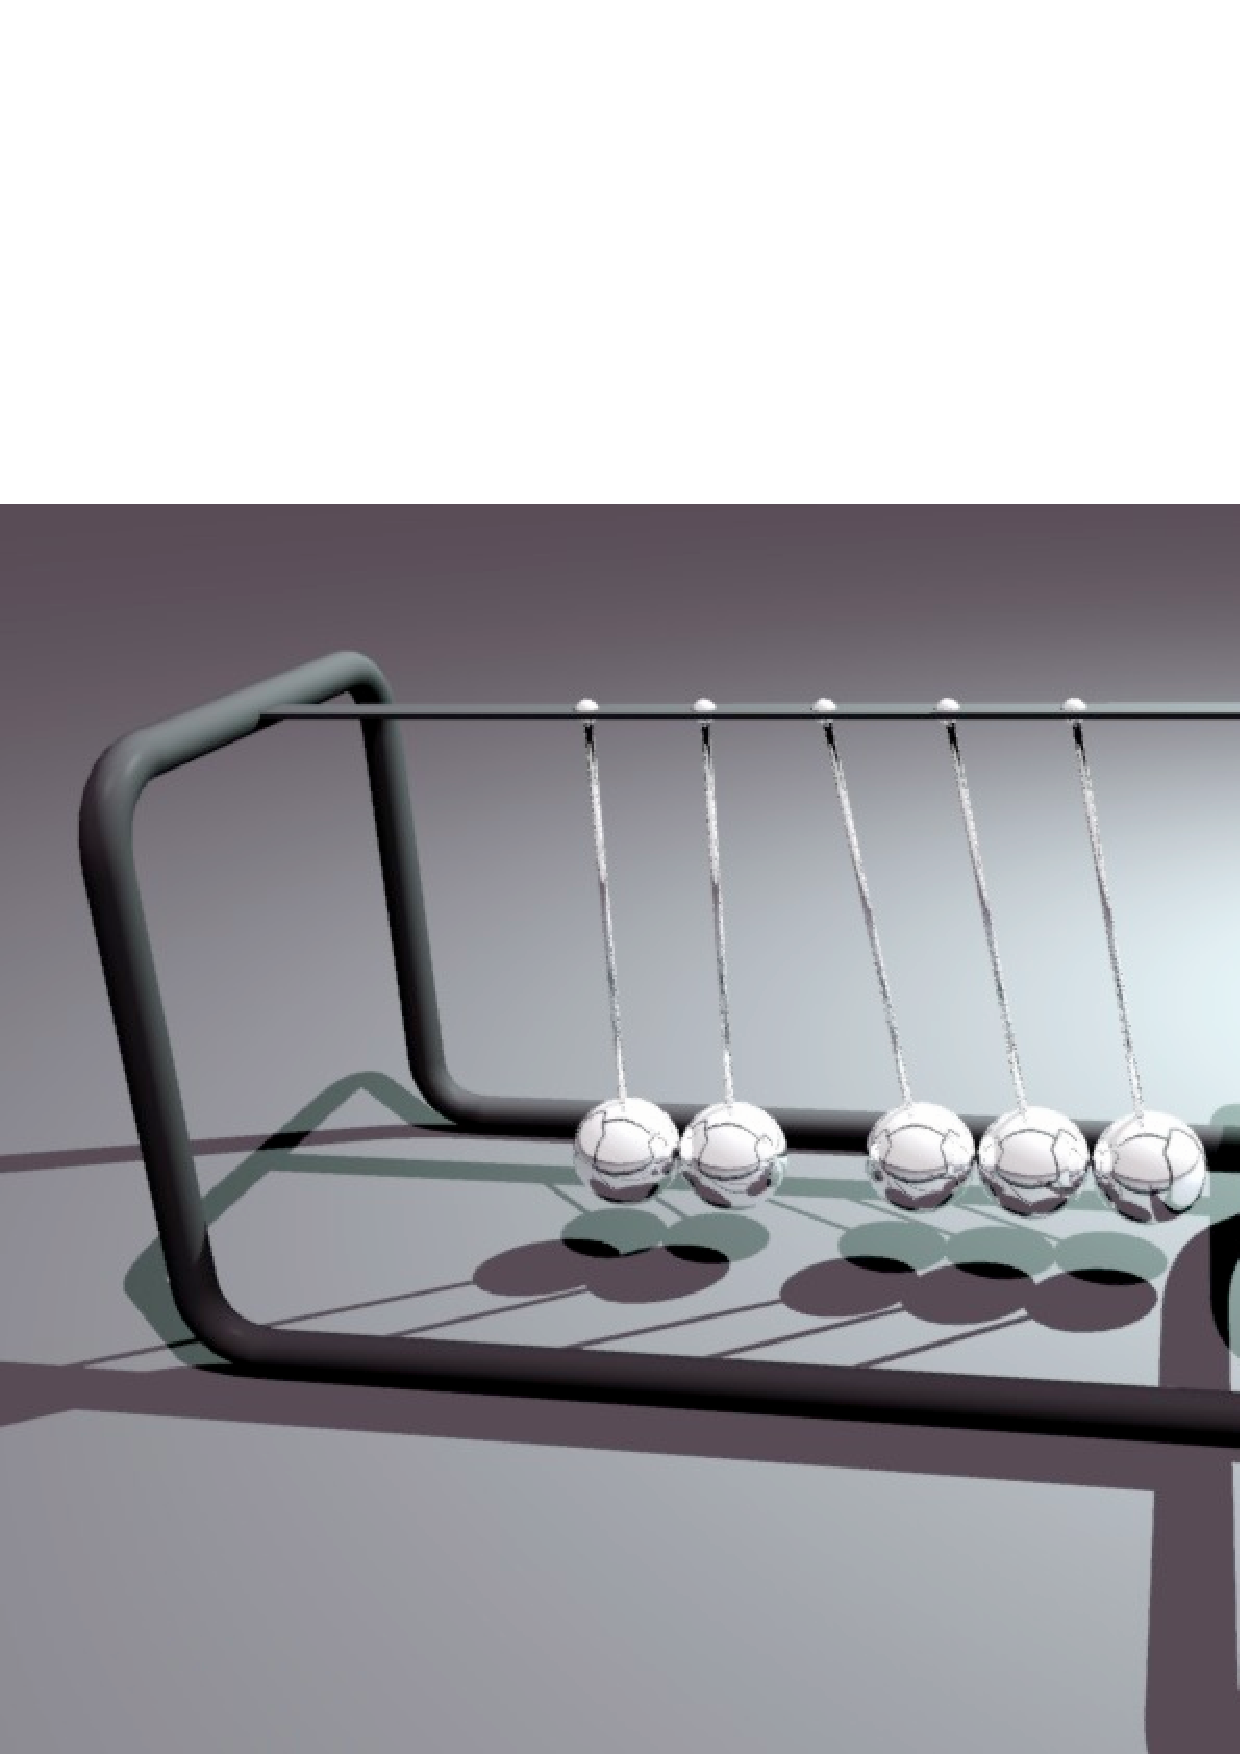
\includegraphics[width=60mm,height=45mm]{figures/cradle3} \hspace{5mm}
            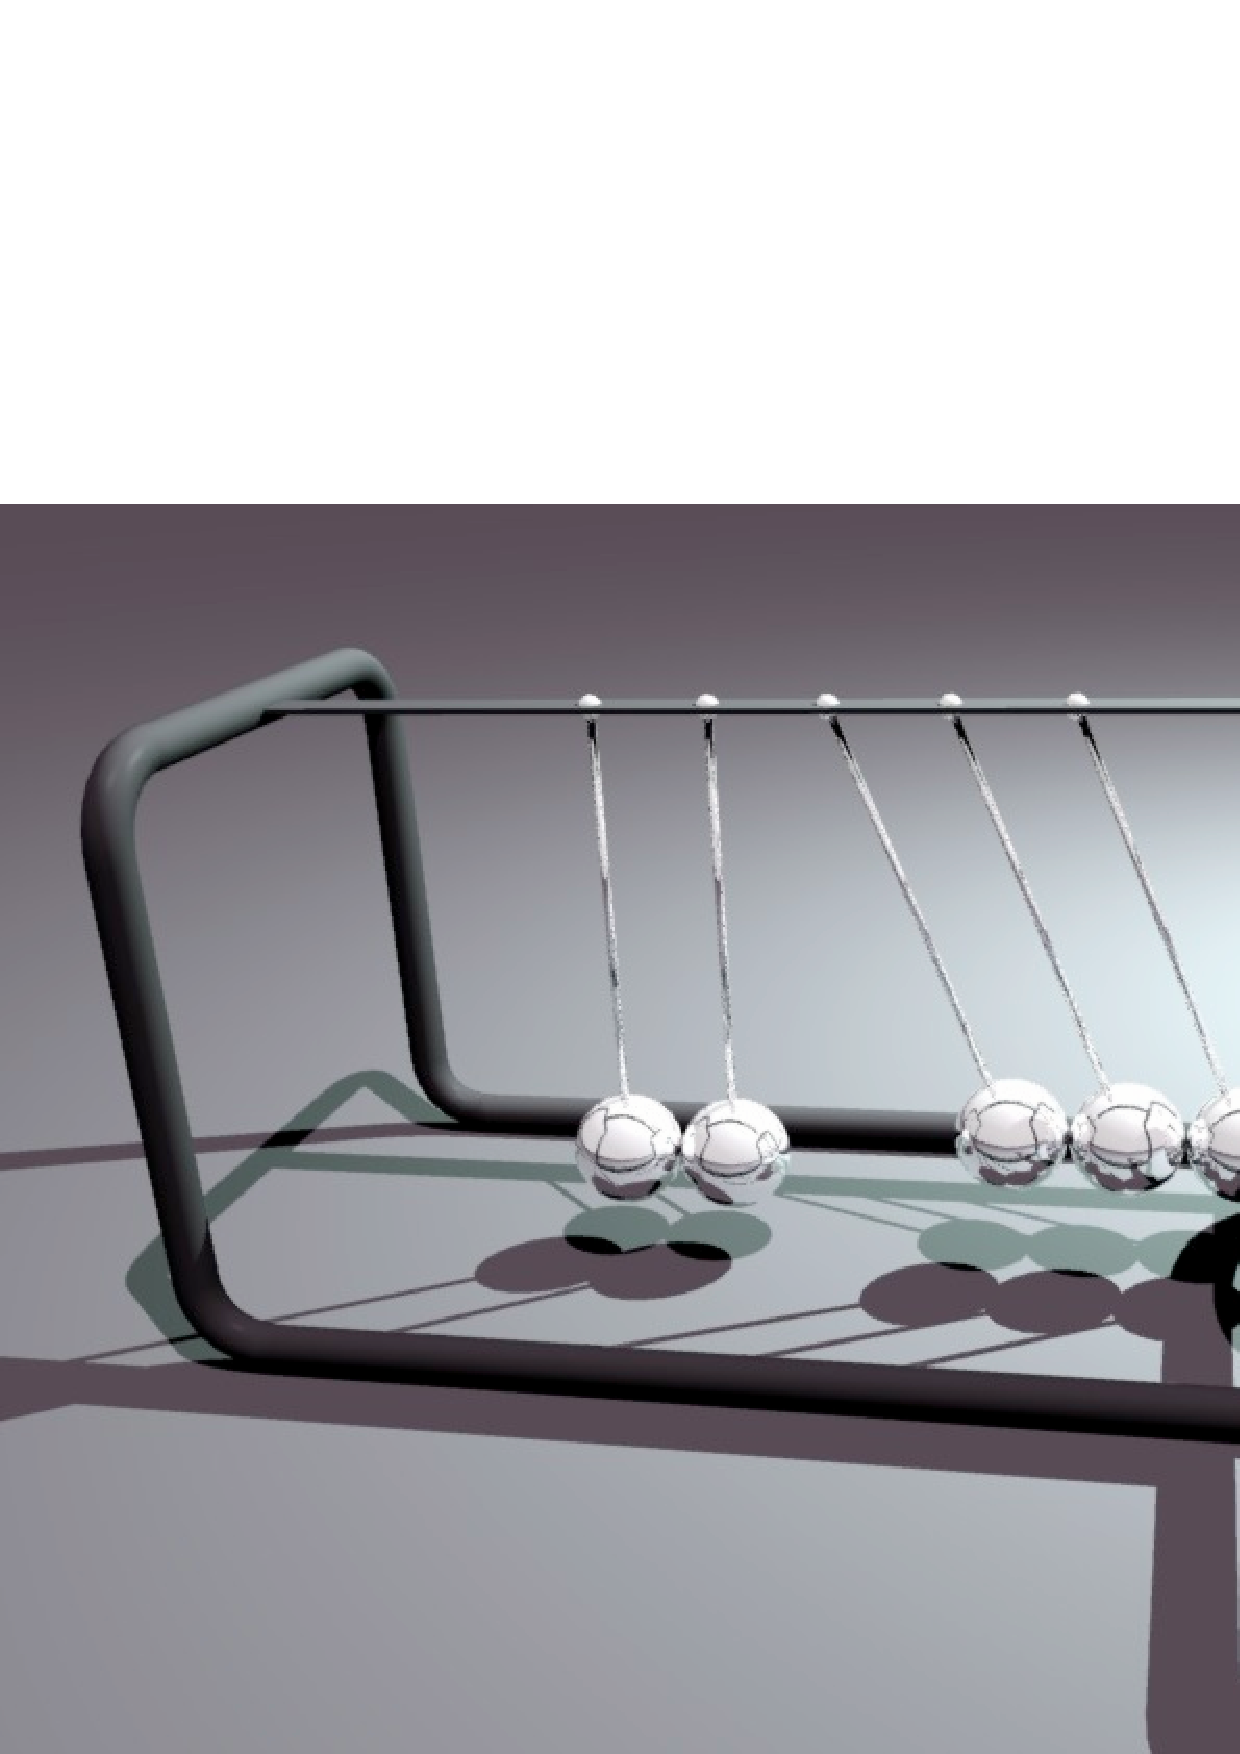
\includegraphics[width=60mm,height=45mm]{figures/cradle4}}
\caption{Animation of Newton's cradle.\label{sampleCradle}}
\end{figure}

The next section shows Newton's cradle in a range of different animations. For full elasticity,
various combinations of one, two and three balls in simultaneous motion are demonstrated, and all
effects observed in a real toy cradle are reproduced. I also simulate what happens if collisions
are not fully elastic: all balls gradually begin to swing, and the sequence of collisions becomes
much more complicated.

Newton's cradle is modelled as five spherical bodies, each with its centre of mass at the centre
of the ball (i.e.\ the wire connecting it to the frame is assumed to be massless). The joint to
the frame is modelled as a `nail' constraint, and the frame itself does not exist in the
simulation. Collision detection is performed not on the basis of the meshes (since these are
polyhedral approximations and not exact spheres), but using a special type of sphere/sphere
constraint which computes its behaviour using the positions of the centres of the balls and their
radii.

For the simulation to work accurately, a very low penetration tolerance must be set. The different
examples are simulated in exactly the same way, independent of the number of balls moving or the
elasticity of collisions.

\subsection{Falling boxes}

\begin{figure}[p]
\centerline{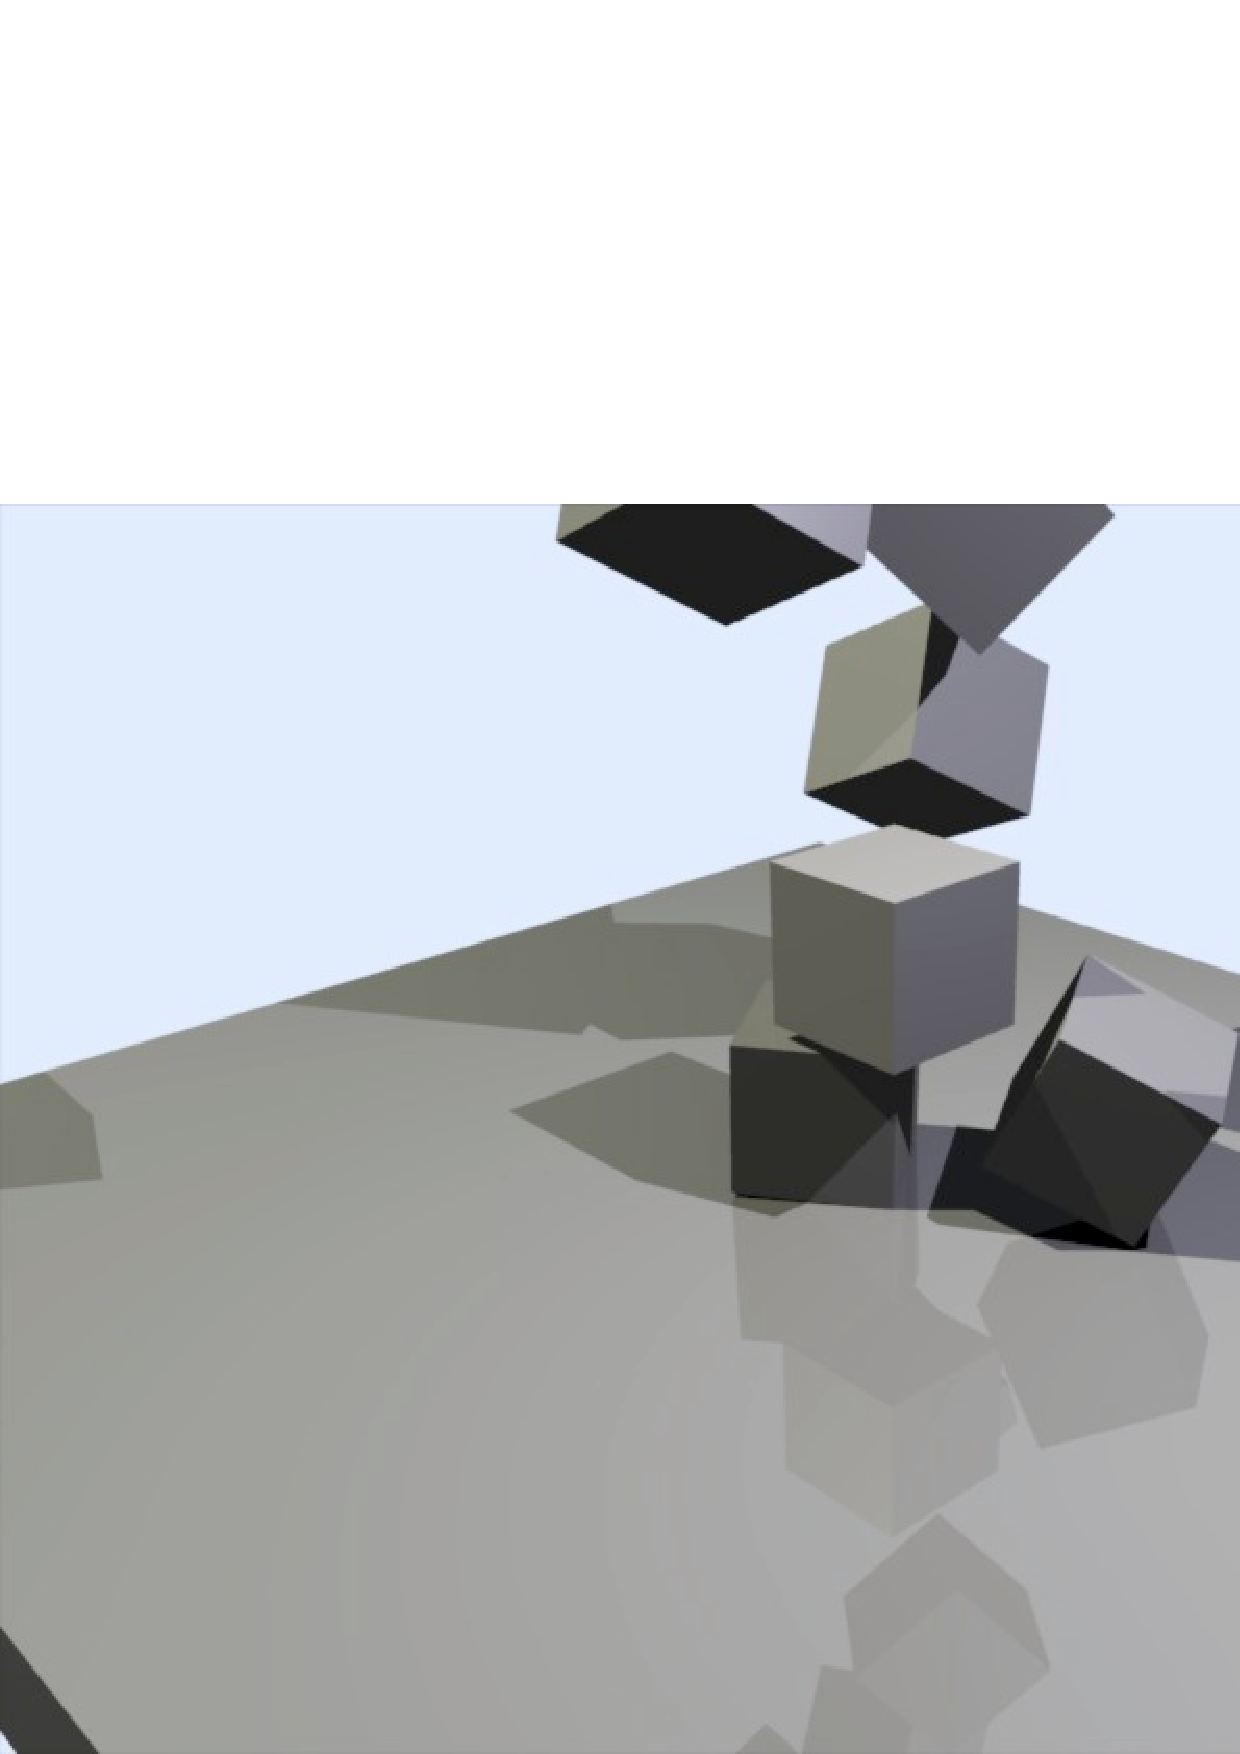
\includegraphics[width=60mm,height=45mm]{figures/boxes1} \hspace{5mm}
            
\includegraphics[width=60mm,height=45mm]{figures/boxes2}}\vspace{5mm}
\centerline{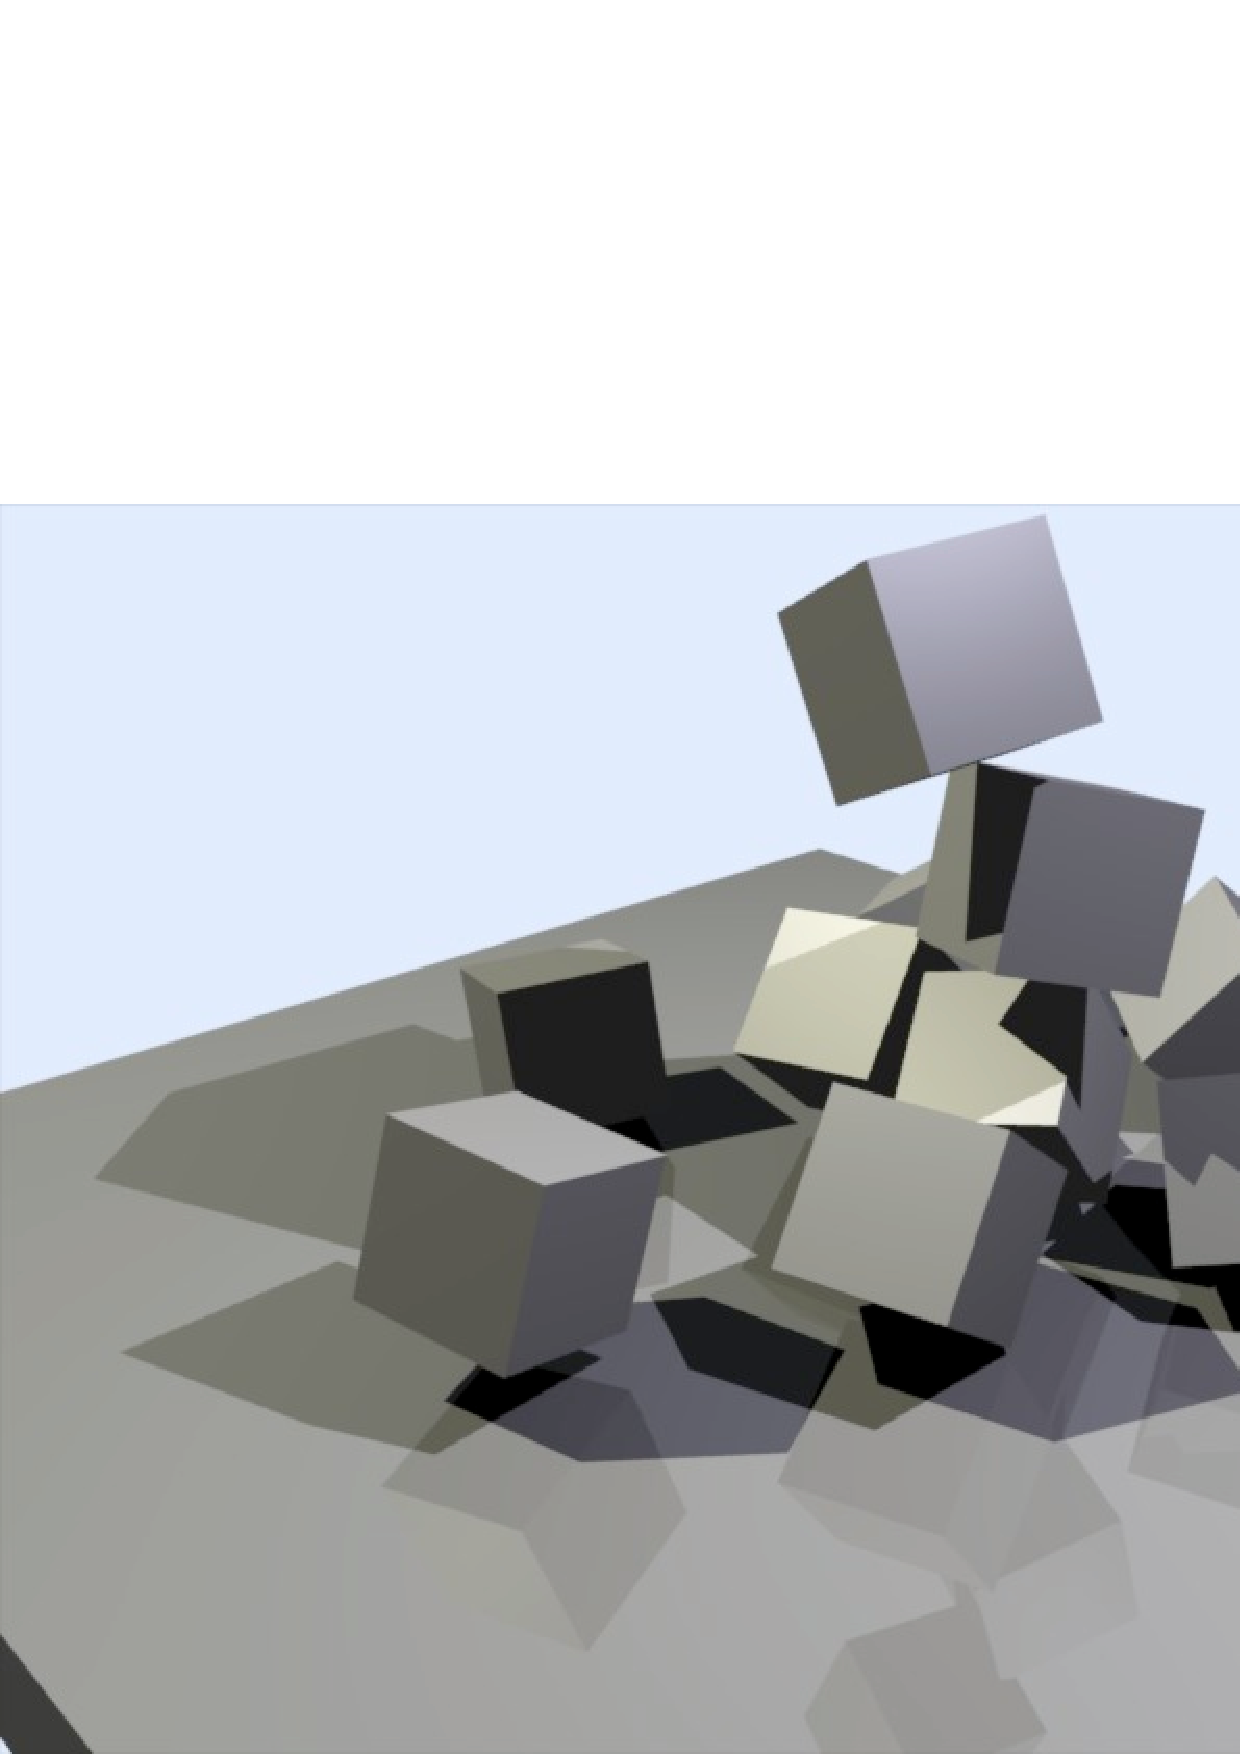
\includegraphics[width=60mm,height=45mm]{figures/boxes3} \hspace{5mm}
            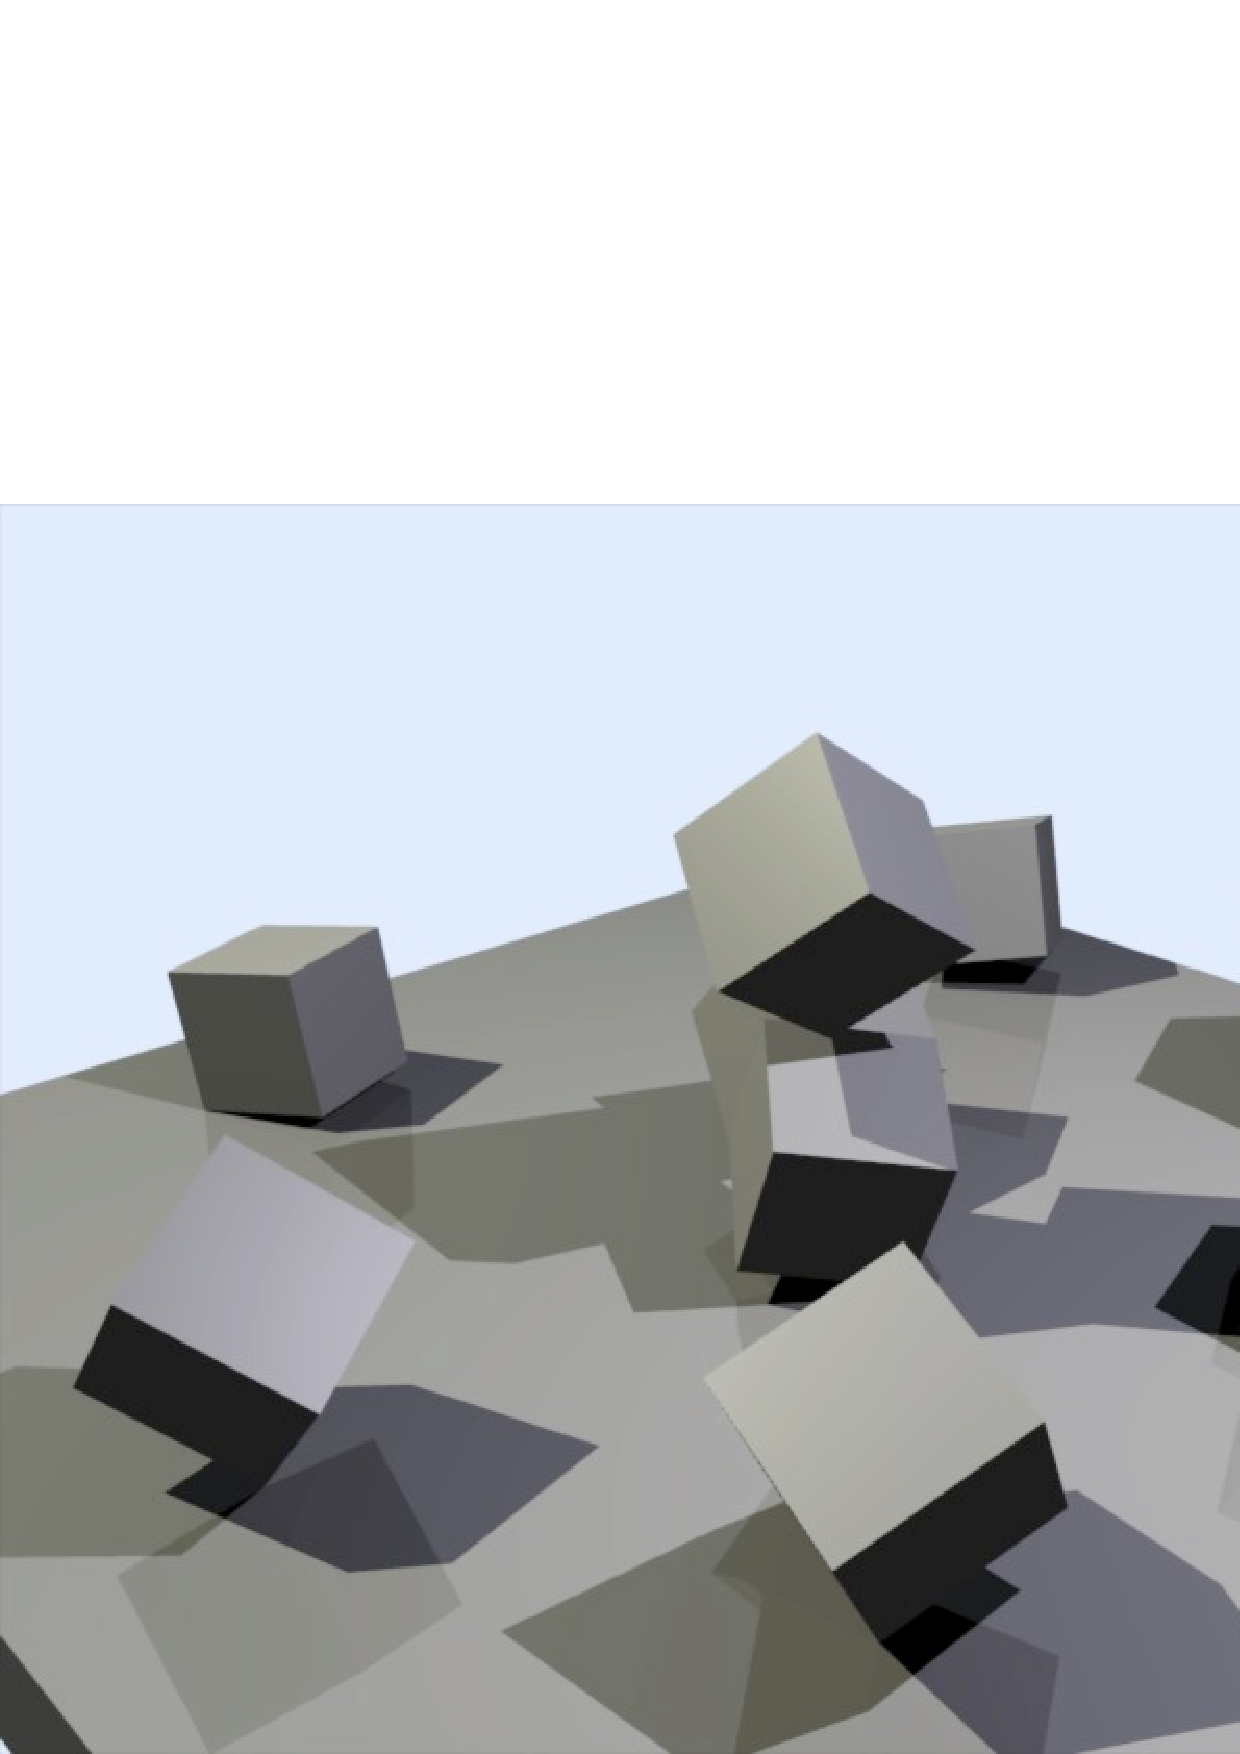
\includegraphics[width=60mm,height=45mm]{figures/boxes4}}
\caption{Animation of ten boxes falling onto a table.\label{sampleBoxes}}
\end{figure}

The third section demonstrates eleven interacting rigid bodies: ten boxes falling onto a table.
The simulation is performed at two different elasticities: one close to what one would expect in
reality ($\varepsilon = 0.2$), and one very bouncy as contrast ($\varepsilon = 1.0$).

Each of the ten boxes is modelled as a symmetric hollow body. All boxes and the table are
specified as meshes in an XML input file. The table is held in place by three `nail' constraints.
These simulations exhibit a range of different collision types: each example starts with a
vertex/face collision when the first box hits the table, and is followed by a sequence of
vertex/face, edge/edge and compound collisions. Whenever a collision cannot be clearly classified
as either vertex/face or edge/edge, the algorithm searches for a plane which contains as closely
as possible the line of intersection between the two colliding meshes. This plane is then used as
the contact plane for computing the impulses and resting contact forces.

The fully elastic version of this simulation looks unrealistic because it behaves as though the
boxes were made of extremely bouncy rubber. The version with elasticity 0.2 is much closer to what
one might expect in a real-life scene, but the contrast between the two is interesting. At the
end of the low-elasticity simulation, several boxes can be seen in a frictionless glide over the
surface of the table. They cannot penetrate the table due to a resting contact force.

\subsection{Alfred falling down stairs}

The final two sections show a humanoid model fall down a straight staircase and a spiral staircase
respectively. I created these simulations to demonstrate a situation which did not require control
of muscular forces (which are hard to control in a simulation~\cite{Green:91}) but were
nevertheless interesting.

The simulation on straight stairs and on the spiral staircase are set up in a very similar way.
Each scene consists of two bodies, a polygon model of the staircase and Alfred himself. In each
case, the staircase is held in place by three `nail' constraints\footnote{It seems intuitively
bizarre that one might make a whole staircase immobile by only three nails, but in the simulation
the magnitude of the forces is, of course, almost irrelevant!}. Alfred is an articulated body
as described in section~\ref{softwareTools}.

All meshes and skeletons are defined in an XML input file. All joints' rotation is restricted in
a way which approximates the anatomical reality. Nonetheless the body sometimes enters poses which,
although they are not impossible, look rather uncomfortable. This is because a pose does not
gradually become more uncomfortable as the limit is approached, but action takes place only at
the limit. The articulated body model would have to be extended to accommodate a notion of
``comfort'' or elastic limits.

For purposes of collision detection, the shape of the Alfred mesh is approximated by 252 little
spheres. The staircase is not approximated. Thus this simulation does not make use of the usual
vertex/face and edge/edge collisions; instead, sphere/face and sphere/edge collisions occur
(on contact with the staircase), and sphere/sphere collisions (on contact between different parts
of the articulated body, e.g.\ the hand against the chest). I found the use of spheres to be the
most reliable technique for such a complicated mesh. Constraint functions for these types of
collision can be derived fairly easily and handled using the usual algorithms for resting and
colliding contact as described in section~\ref{collisionHandling}.

The camera movement and lighting was set up in Blender. After importing the simulation results,
the animation was rendered using Blender's internal renderer/raytracer. Some of the mesh
deformations look strange; this is unrelated to the simulation, but must be blamed on my lack of
3D art skills!

\begin{figure}[p]
\centerline{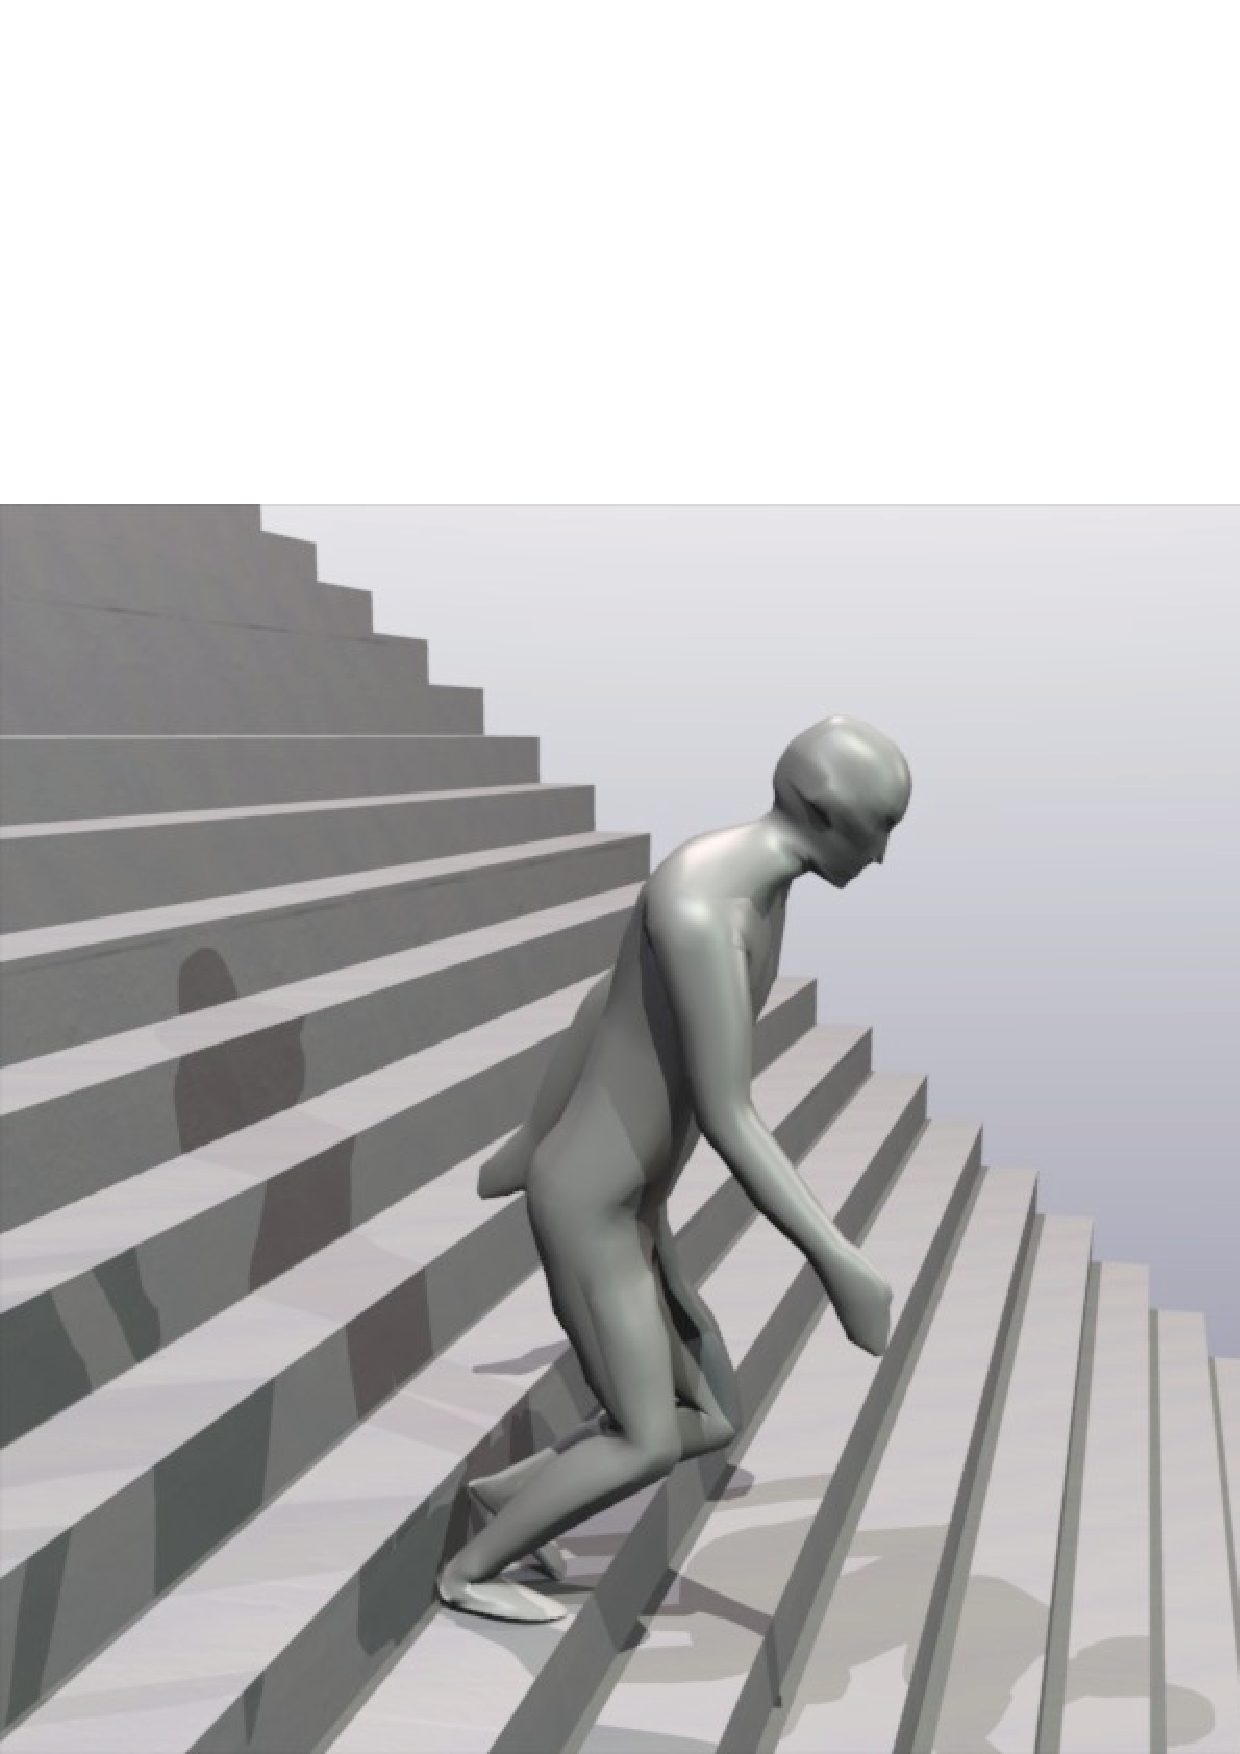
\includegraphics[width=60mm,height=45mm]{figures/stairs1} \hspace{5mm}
            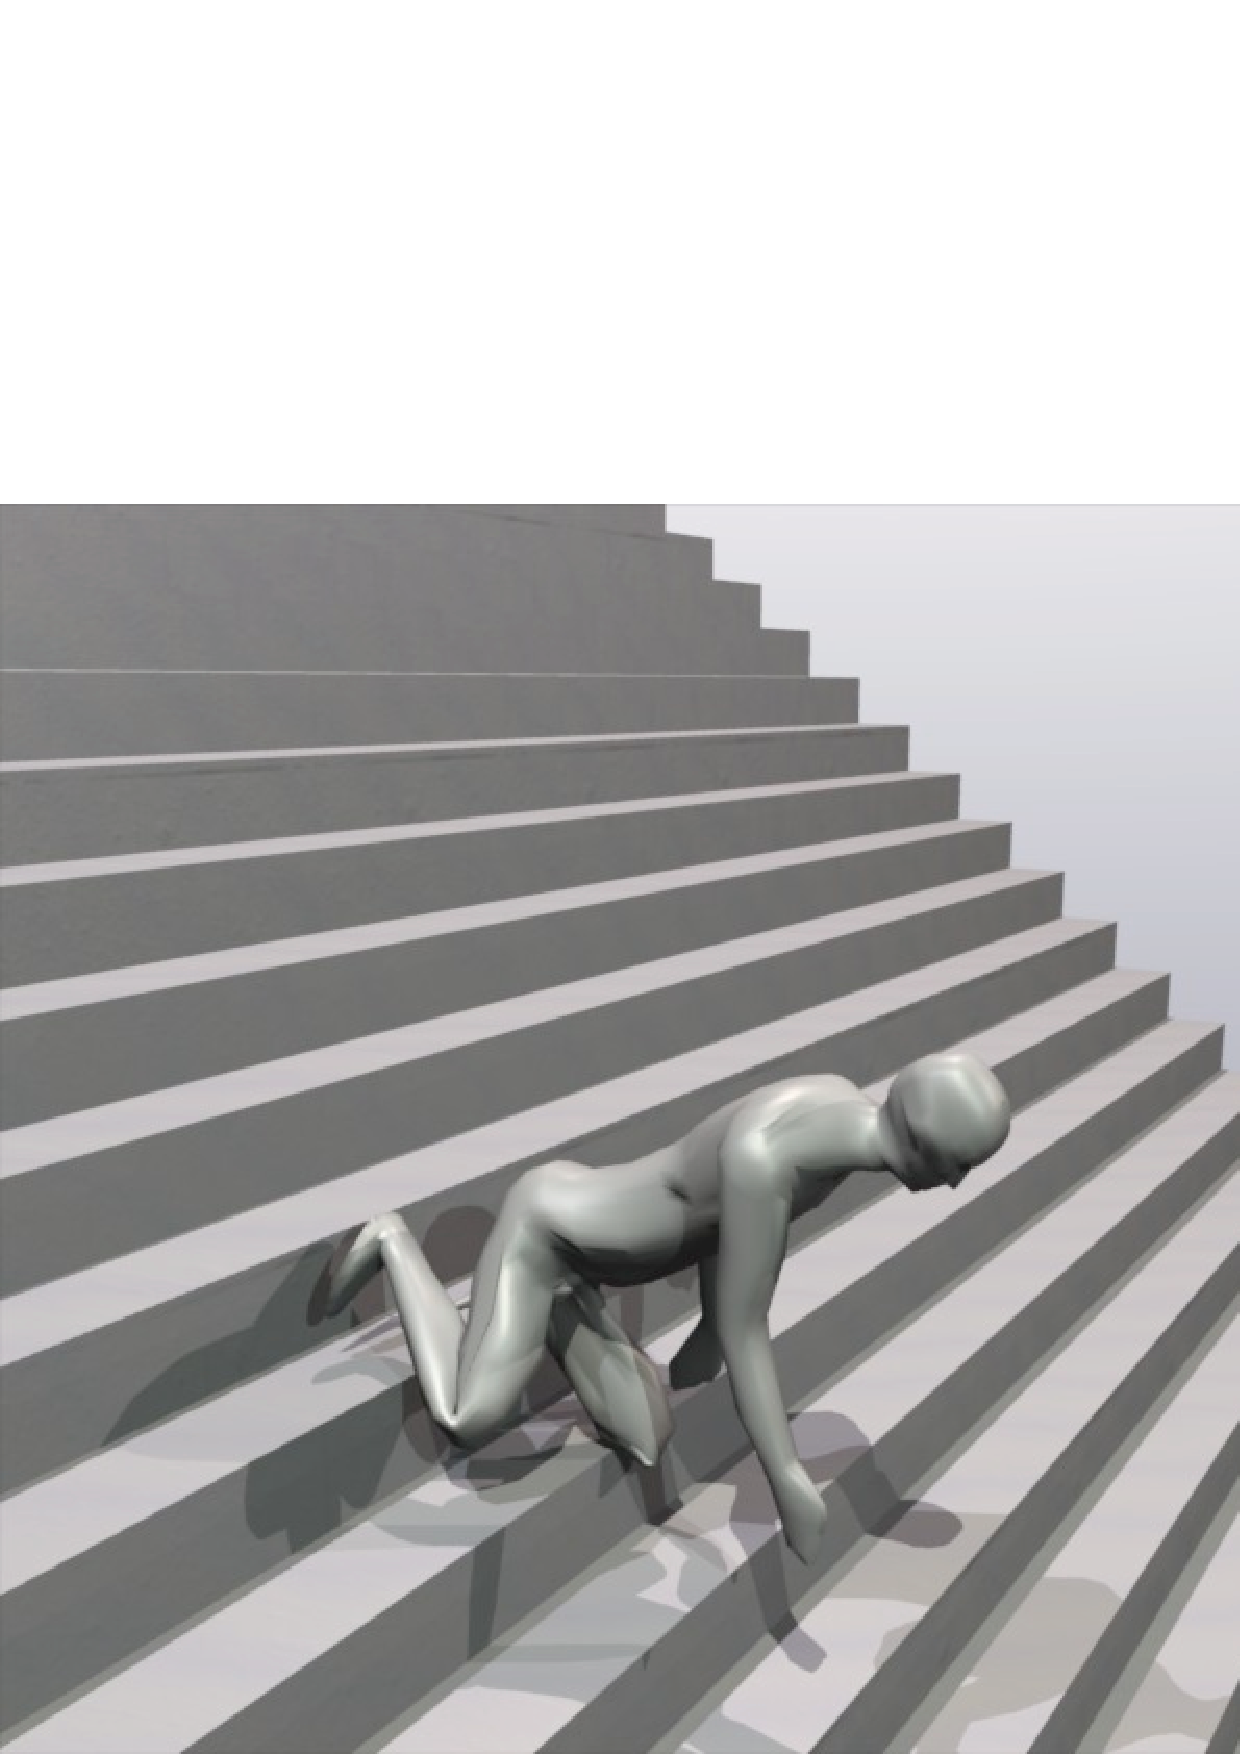
\includegraphics[width=60mm,height=45mm]{figures/stairs2}}\vspace{5mm}
\centerline{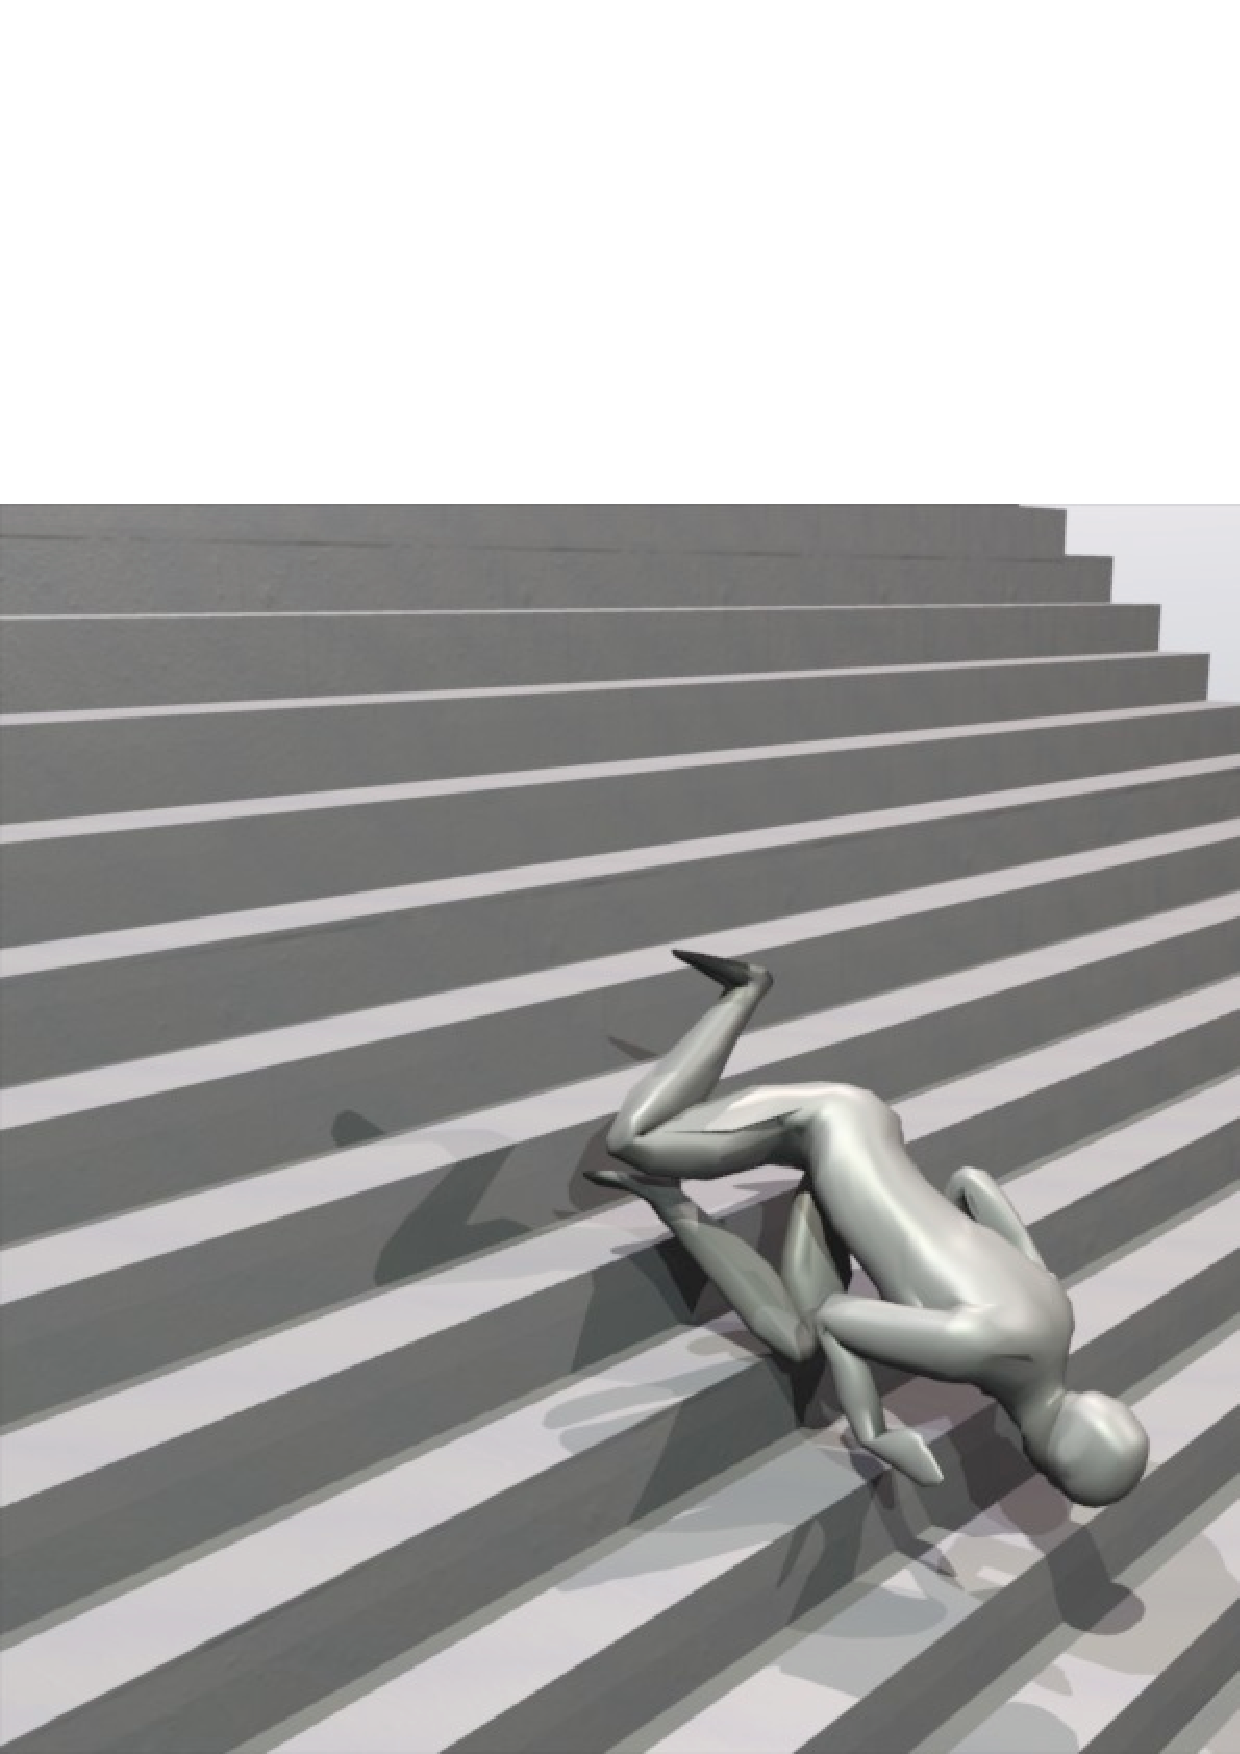
\includegraphics[width=60mm,height=45mm]{figures/stairs3} \hspace{5mm}
            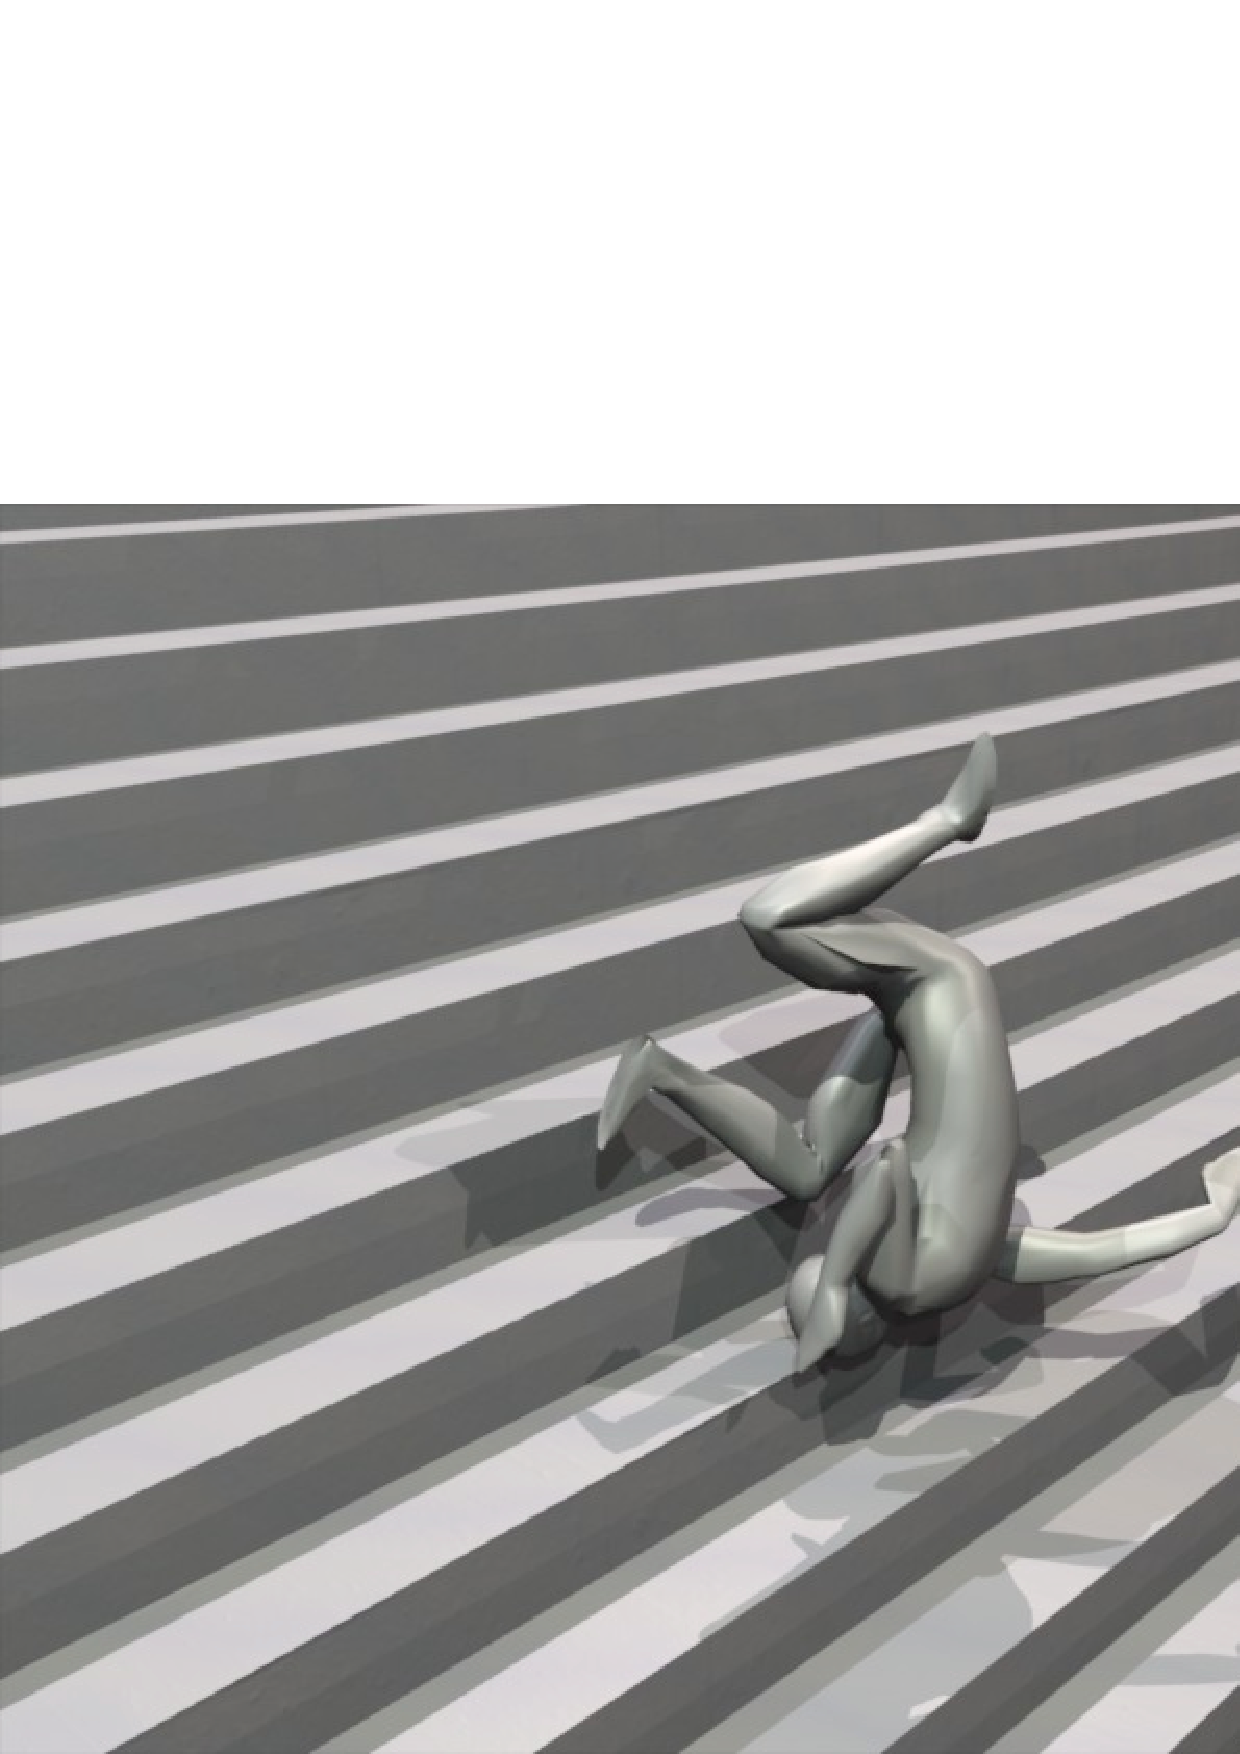
\includegraphics[width=60mm,height=45mm]{figures/stairs4}}
\caption{Animation of Alfred falling down a set of stairs.\label{sampleStairs}}
\end{figure}

\begin{figure}[p]
\centerline{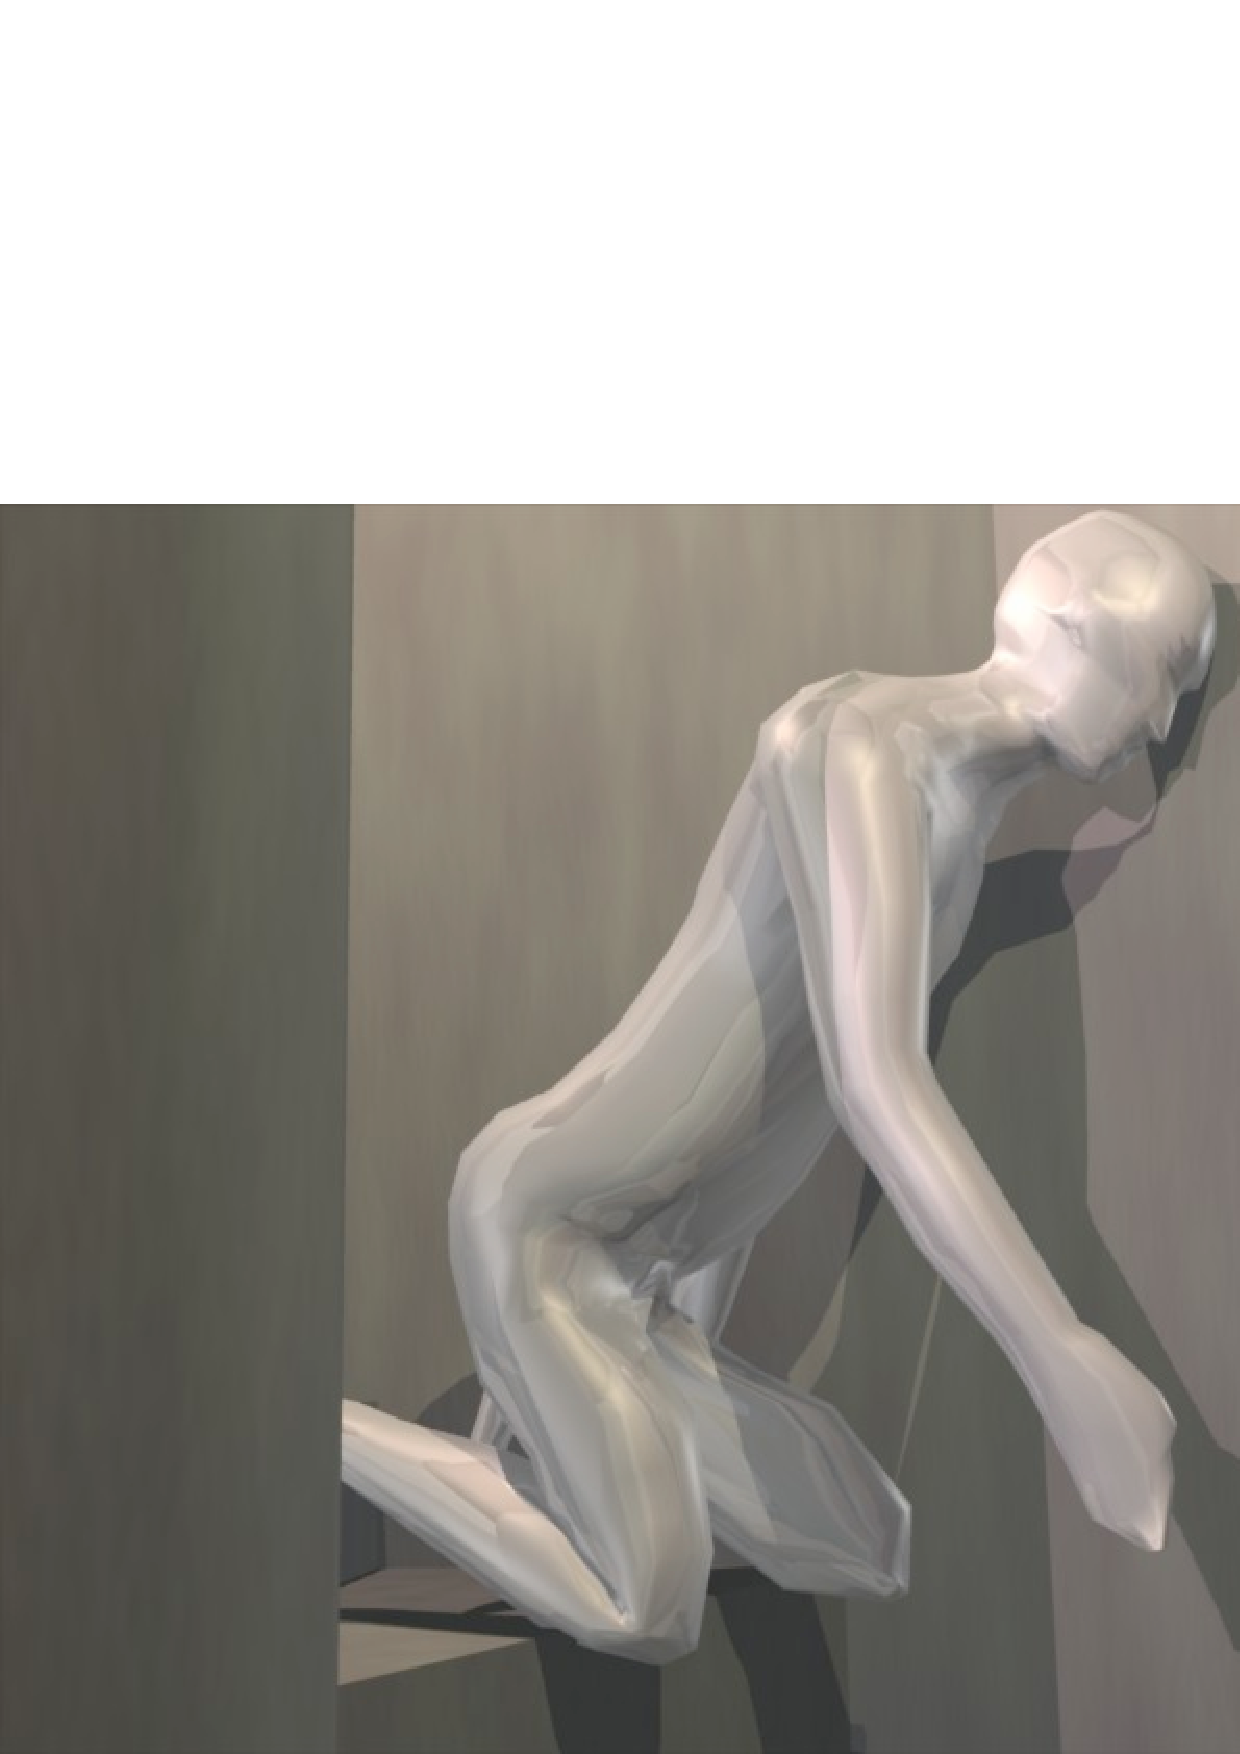
\includegraphics[width=60mm,height=45mm]{figures/spiral1} \hspace{5mm}
            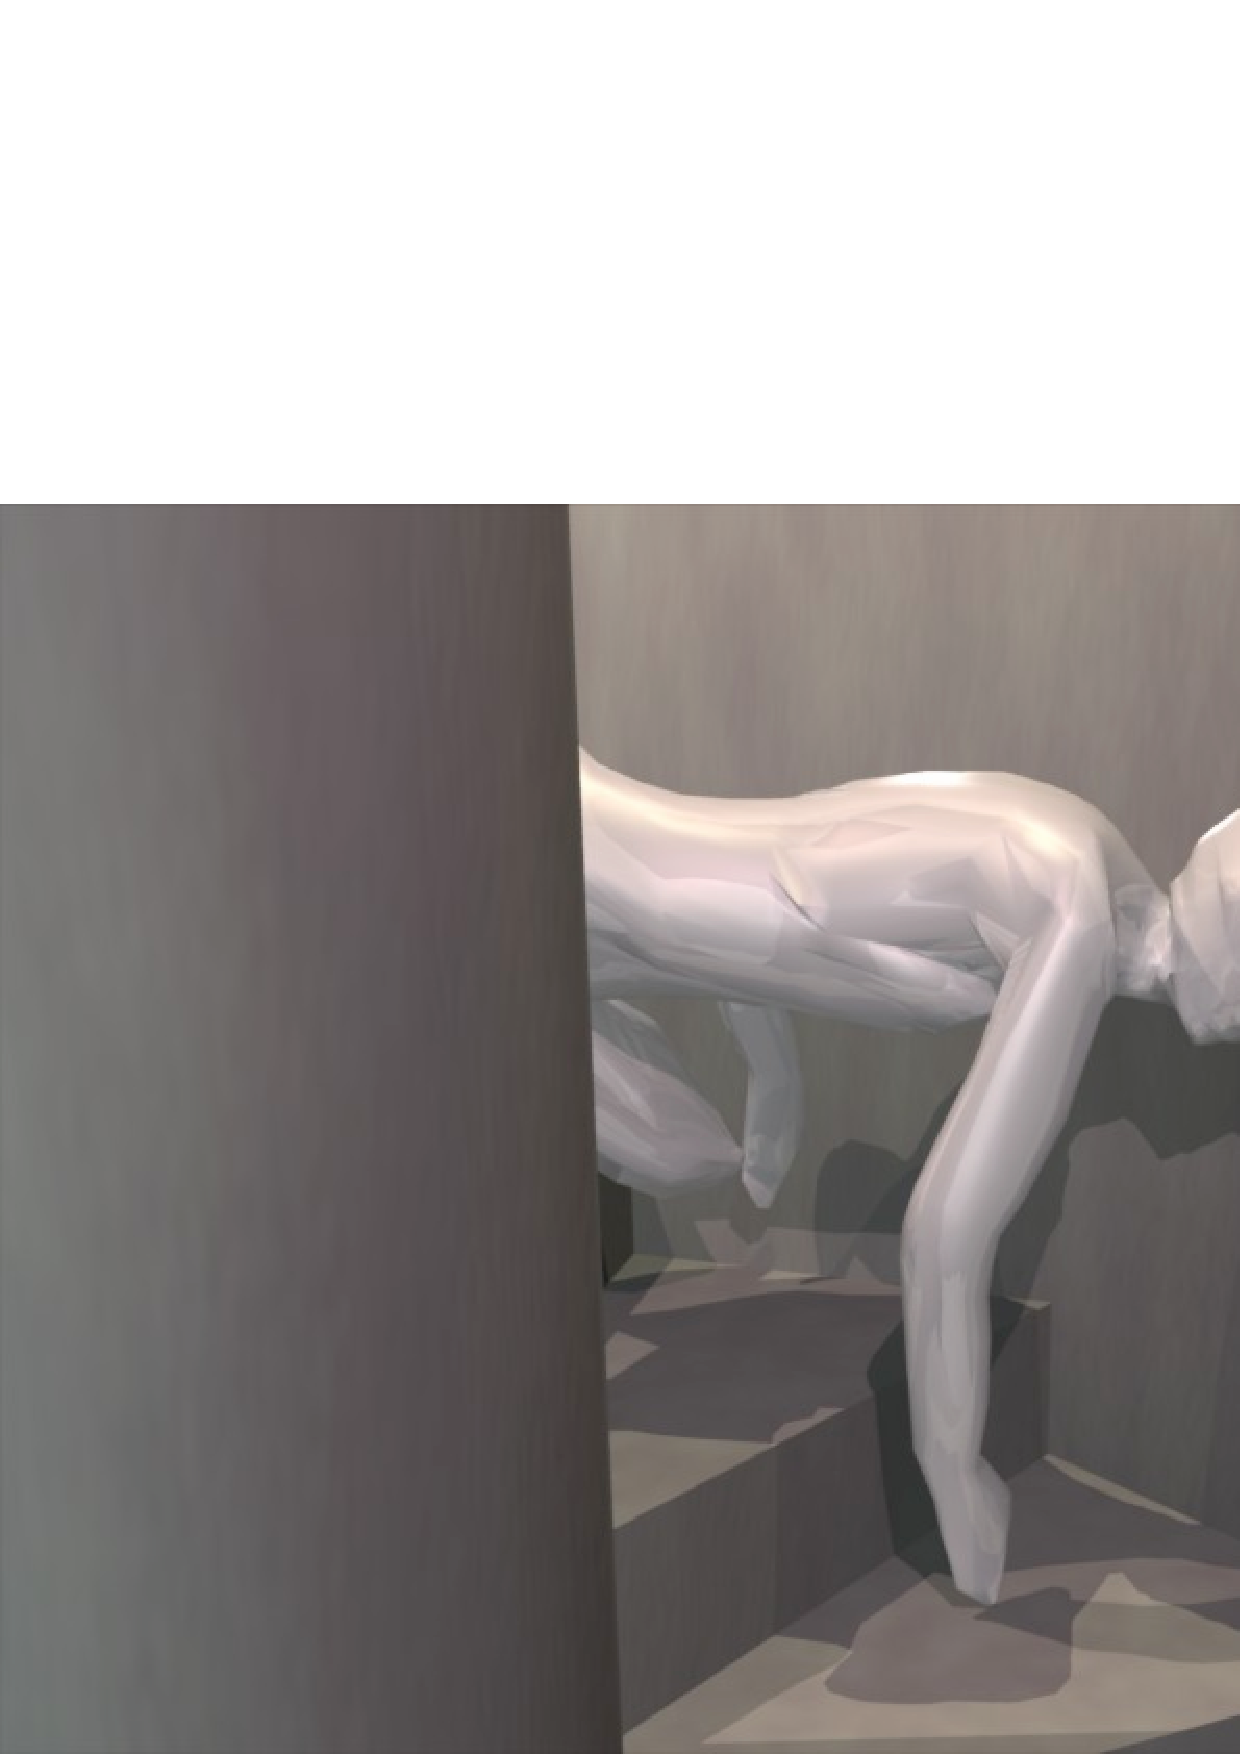
\includegraphics[width=60mm,height=45mm]{figures/spiral2}}\vspace{5mm}
\centerline{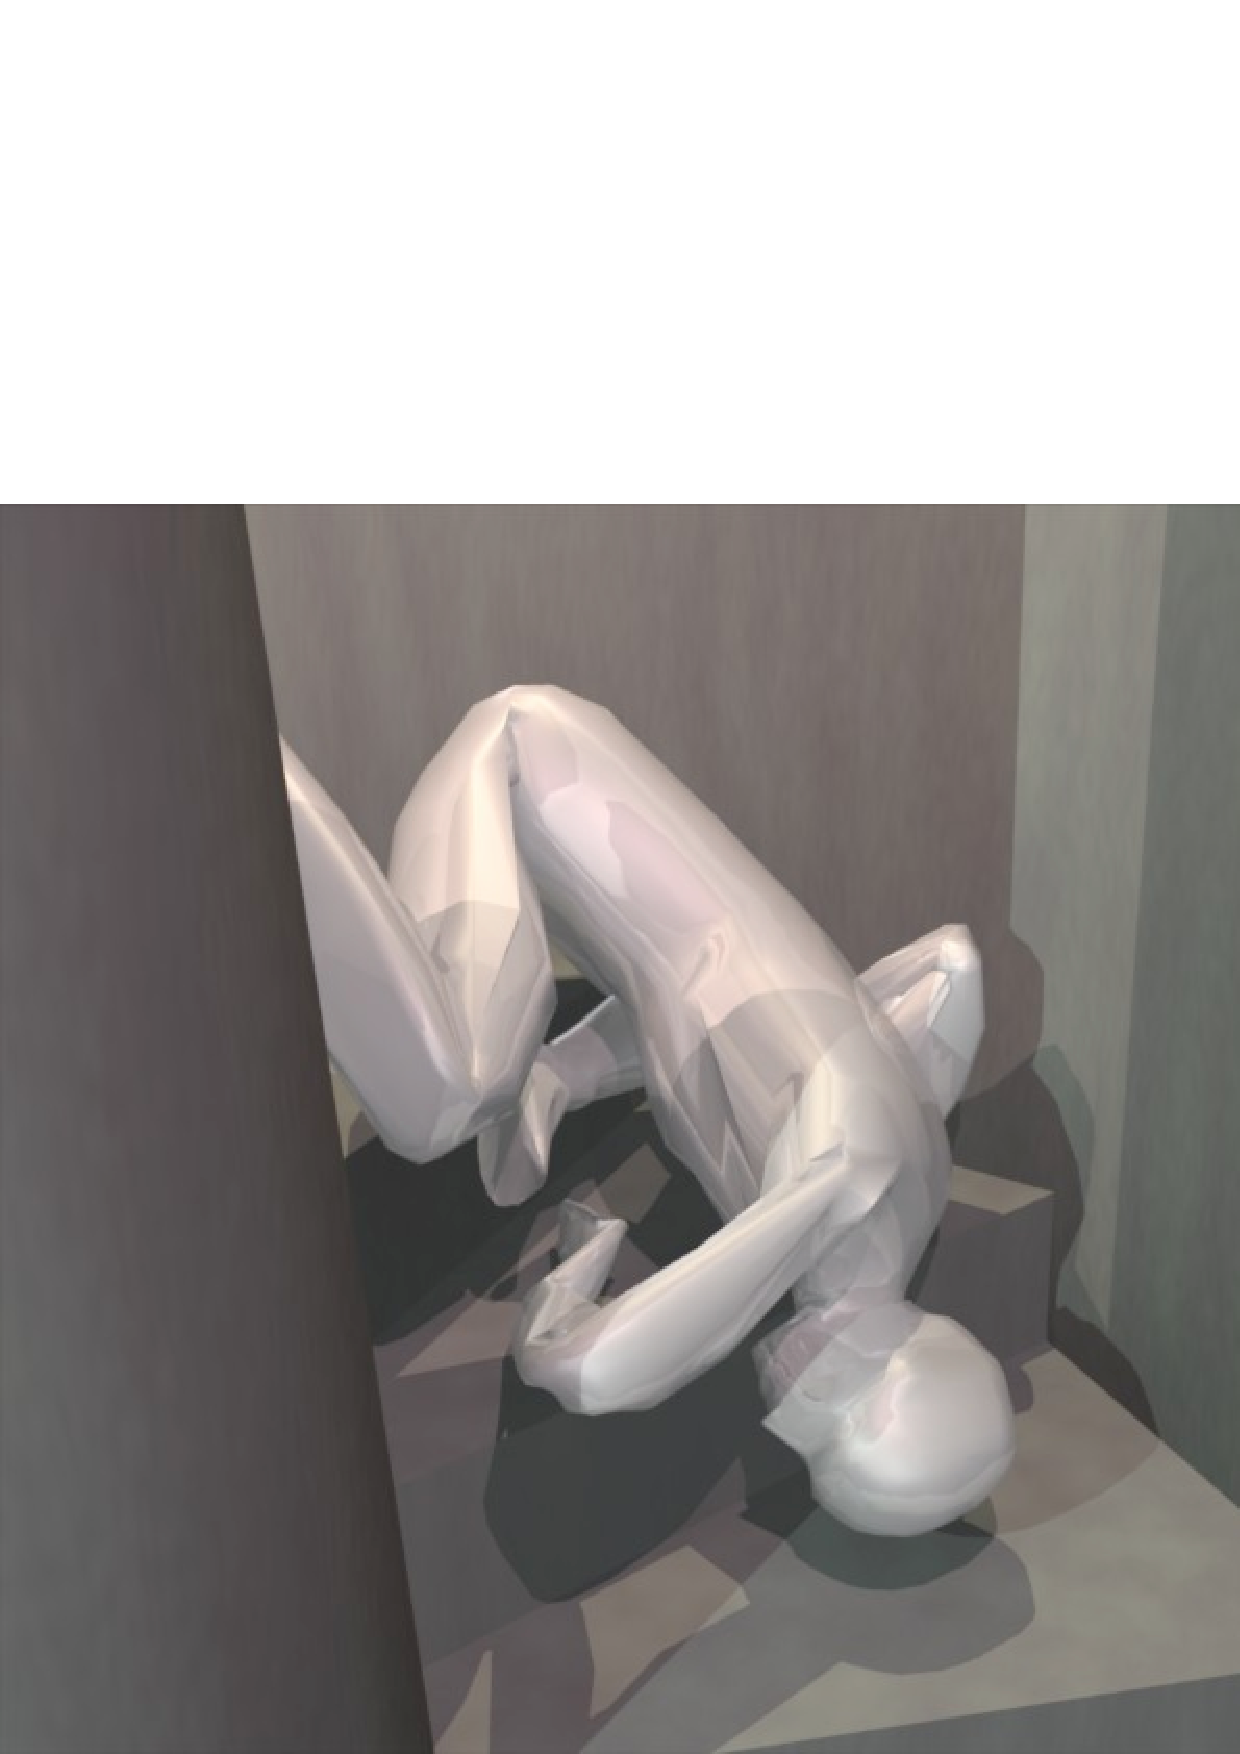
\includegraphics[width=60mm,height=45mm]{figures/spiral3} \hspace{5mm}
            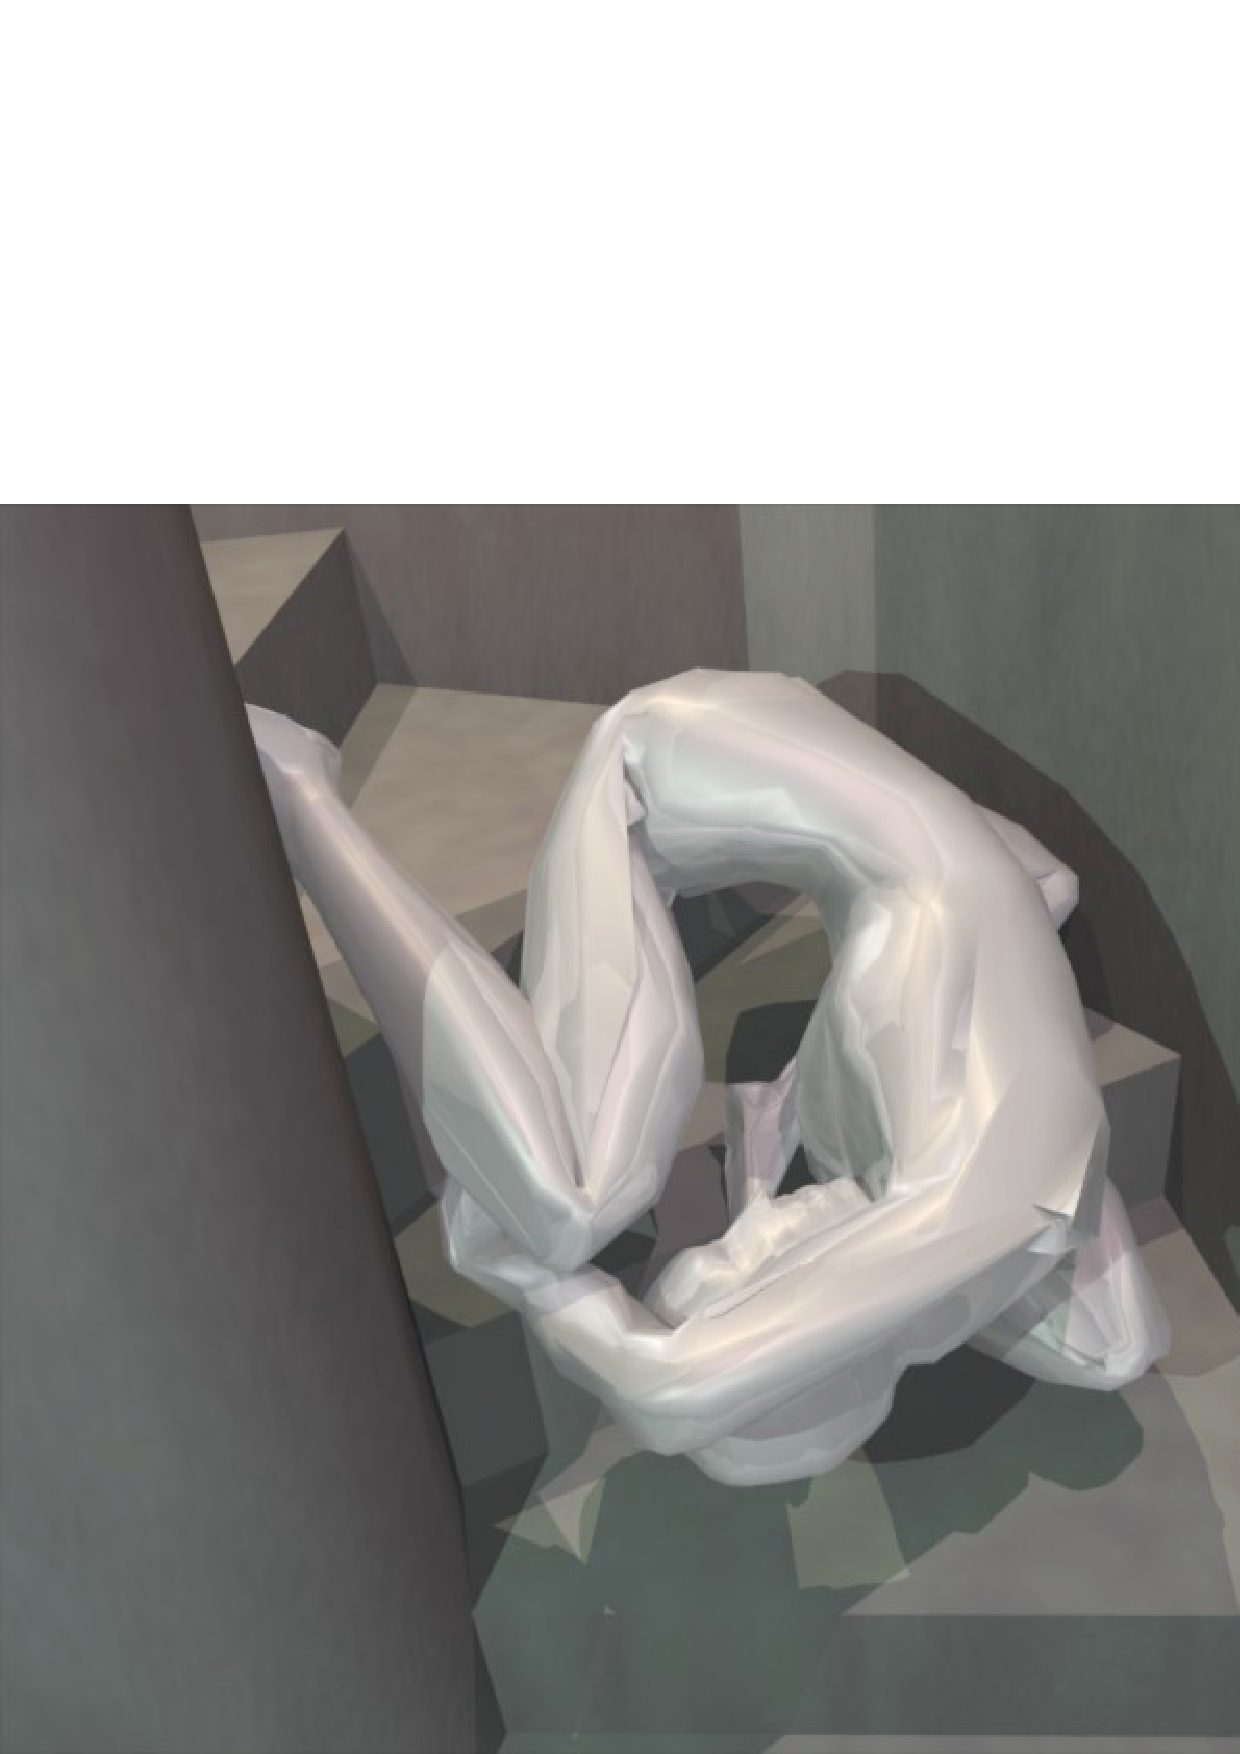
\includegraphics[width=60mm,height=45mm]{figures/spiral4}}
\caption{Animation of Alfred tumbling down a spiral staircase.\label{sampleSpiral}}
\end{figure}


\chapter{Conclusions}
\section{Successes}

In this project I have successfully created a general-purpose application which simulates
the dynamic behaviour of many different mechanical systems. In particular, it handles all
features necessary to animate articulated characters like humans or animals: an
arbitrary-shaped exterior, a skeleton with many different types of joints, and
collisions with other bodies. I have quantitatively verified the accuracy of the simulation
results for simple mechanical systems, and demonstrated that the program produces
realistic-looking animations in more complicated scenes involving a
model of a human character.

All requirements given in the project proposal have been met, except for the simulation of friction,
which was ruled out at an early stage because it is too complicated. All other features were
realized at a high quality standard. The implementation is carefully designed to use refined
algorithms which 
\begin{itemize}
\item keep numerical errors very small, doubtlessly within the bounds acceptable even for
    ambitious computer graphics purposes;
\item give the simulation a high degree of stability and reliability;
\item allow a reasonable run-time performance which can be traded off against the required
    accuracy by adjusting parameters.
\end{itemize}

The technology of this project is close to current research, and carrying it out
required some algorithms which I could not find in any of the publications I searched. I therefore
had to newly invent several algorithms, which took several weeks longer than anticipated in
the original schedule. However, I succeeded in adapting my management strategy
to the uncertainties facing this project, so that it could be completed in an organized way.

\section{Limitations}

There are only few explicit approximations in my simulation algorithms; this means that if they
were to be run using arbitrary-precision arithmetic and arbitrarily small time steps, the exact
physical behaviour would be obtained. The exceptions are:
\begin{itemize}
\item Given a triangle mesh and the density of a body, I currently approximate its mass and moment
    of inertia using a simple heuristic. For a better simulation, this should be
    replaced by an exact analysis of the geometric properties~\cite{Mirtich:96}.
\item Simple collisions (vertex/face and edge/edge cases) can be handled in an exact way, but
    more complicated collision geometries are currently approximated by planes or bounding
    spheres. This produces plausible-looking but slightly incorrect animations. Ideally,
    exact handling of any sort of collision would be desirable, but I am unsure whether such
    an algorithm exists.
\item As mentioned previously, static and sliding friction have been completely ignored.
    Algorithms to simulate these exist, but they are complicated~\cite{Baraff:PhD}.
\end{itemize}

Even with these added features, my program would not be a ready-to-market product. It particularly
lacks user-friendliness: there are several simulation parameters (tolerances and error thresholds)
which need to be configured differently depending on the situation in order to obtain good
results. Ideally the program should be able to determine these automatically. A higher execution
speed would also be beneficial, since the current cost~-- in my test cases, up to an hour of CPU
time per second of simulation time~-- limits productivity.

\section{Summary and outlook}

In summary, I consider this project a clear success. I am glad to have chosen such an ambitious
project because it was personally rewarding: in particular, the lack of existing algorithms
forced me to contemplate the background theory in great detail, which has given me a good
understanding of the subject area.

There are not many decisions that I would have taken differently in retrospect. In the schedule I
should have left more time for understanding the theory; I had thought there would be a simple,
``obvious'' way of realizing articulated bodies, rather than having to deal with constraints. This
meant I massively underestimated the problem. I would have also avoided the design mistake
mentioned in section~\ref{algorithmImplementation}.

The application is not yet user-friendly enough for general use, but with some additional effort
it might gain this potential. I can envisage working on it beyond the frame of this project,
and will consider the possibility of publishing some of the new algorithms to a wider audience.

I would like to thank Dr.~Brett Saunders~\cite{Saunders} and Dr.~Neil Dodgson (supervisor) for
their ideas and discussions, particularly in the early phase of this project.

\vspace{20pt}
\centerline{\texttt{http://www.maniation.com/}}

\begin{appendix}
\chapter{Notation}
\begin{tabular}{@{}lll@{}}
\renewcommand{\baselinestretch}{1.3}\small\normalsize
$a$ & italic Latin letter & scalar\\
$\theta$ & italic Greek letter & angle\\
\ve{a} & boldface Greek/Latin letter & column vector\\
\ve{0} & boldface figure 0 & null vector (of appropriate dimension)\\
\m{M} & sans serif upper-case letter & matrix\\
\m{1} & sans serif figure 1 & identity matrix (of appropriate dimensions)\\
\q{q} & sans serif lower-case letter & quaternion\\
$\dot{c}$ & dot & first derivative with respect to time\\
$\ddot{c}$ & double dot & second derivative with respect to time\\
$\m{J}^T$ & superscript $T$ & matrix transpose\\
$\m{M}^{-1}$ & superscript $-1$ & matrix or quaternion inverse (equation~\ref{quatInverse})\\
$\overline{\q{q}}$ & bar & quaternion conjugate (equation~\ref{quatConjugate})\\
$\norm{\ve{a}}$ & norm & vector or quaternion magnitude (equation~\ref{quatMagnitude})\\
$\tilde{\ve{a}}$ & tilde & corresponding quaternion (equation~\ref{vectorToQuat})\\
$\dual{\ve{a}}$ & asterisk & dual tensor (equation~\ref{dualTensor})\\
$\ve{a}\times\ve{b}$ & cross & vector cross product\\
$\ve{a}\cdot\ve{b}$ & dot & inner product\\
$\Re(\q{q})$ & real & real part of a quaternion\\
\end{tabular}
\vspace{10pt}

Given any vector $\ve{a} = (a_1, a_2, a_3)^T$, we define its dual
tensor, written as a $3\times3$ matrix, to be
\begin{equation}\label{dualTensor}
\dual{\ve{a}} = \left[\begin{array}{ccc}
    0 & -a_3 & a_2 \\ a_3 & 0 & -a_1 \\ -a_2 & a_1 & 0
    \end{array}\right]
\end{equation}
(see \cite{RHB:02,BaraffWitkin:97} and also Kalra~\cite{Kalra:95}, who defines it to be
the transpose of the expression above).
The dual allows us to rewrite a vector cross product as a matrix multiplication:
\begin{equation}
\ve{a}\times\ve{b} = \dual{\ve{a}}\,\ve{b}
\end{equation}
Note that $(\dual{\ve{a}})^T = -\dual{\ve{a}}$.

Let us also recall some basic identities of vector and matrix algebra~\cite{RHB:02}:
\begin{eqnarray*}
\ve{a}\times\ve{a} & = & \ve{0}\quad\mathrm{(the~null~vector)} \\
\ve{a}\times\ve{b} & = & -\ve{b}\times\ve{a} \\
\ve{a}\times(\ve{b} + \ve{c}) & = & \ve{a}\times\ve{b} + \ve{a}\times\ve{c} \\
\ve{a}\cdot\ve{b} & = & \ve{b}\cdot\ve{a} \\
\ve{a}\cdot\ve{b} & = & \ve{a}^T\,\ve{b} \\
\ve{a}\cdot(\ve{b} + \ve{c}) & = & \ve{a}\cdot\ve{b} + \ve{a}\cdot\ve{c} \\
\ve{a}\cdot(\ve{b}\times\ve{c}) & = & \ve{b}\cdot(\ve{c}\times\ve{a}) \\
    & = & \ve{c}\cdot(\ve{a}\times\ve{b}) \\
\ve{a}\times(\ve{b}\times\ve{c}) & = &
    \ve{b}(\ve{a}\cdot\ve{c}) - \ve{c}(\ve{a}\cdot\ve{b}) \\
(\m{A}\m{B})\m{C} & = & \m{A}(\m{B}\m{C}) \\
\m{A}(\m{B} + \m{C}) & = & \m{A}\m{B} + \m{A}\m{C} \\
(\m{A}\m{B})^T & = & \m{B}^T\m{A}^T \\
\m{A}\m{A}^{-1} = \m{A}^{-1}\m{A} & = & \m{1}\quad\mathrm{(the~identity~matrix)}
\end{eqnarray*}


\chapter{Simulation examples (CD-ROM)\label{cdrom}}

The CD-ROM accompanying this dissertation contains a video file (in MPEG-1 format) demonstrating
many features of my simulation program. The same content may be obtained from the project web site
at \texttt{http://www.maniation.com/}\footnote{\emph{maniation} is a simple anagram of
\emph{animation}, and also contains the word \emph{mania}.}. The video shows a number of raytraced
renderings of animations produced by simulation. There is also a sub-directory containing each
scene as an individual file, to facilitate detailed examination.

The following sections give a brief overview of how each simulation was created, and points out
aspects that can be observed.

\section{Pendulum systems}

This section demonstrates the animation of a double pendulum (a rigid pendulum with a second one
attached to its end), and its extension to three, eight and 25 segments. The double pendulum is
a commonly studied system in physics; although it does not have an exact analytic solution, an
approximate solution can be found for small angles. In this case, one finds that the resulting
movement is the sum of two simple harmonic oscillations at different frequencies, resulting in
a mysterious-looking swinging movement.

The double, triple and eight-part pendulums are set up in a very similar way. Each segment is
modelled as a rigid cylinder with constant density. The top end of the top segment is held in
place by a `nail' constraint. Each pair of adjacent segments is connected by a ball-and-socket
joint. Initially, all segments are at rest, the first segment is rotated by 45 degrees
anticlockwise from the equilibrium position, and all other segments hang straight down.

The simulation does not employ an XML input file; instead, the objects representing the bodies
and the constraints are directly created by the Java test case. The simulation results were
exported to Blender and rendered using the internal renderer and orthographic projection.
I also performed a Fourier transform on the results of the double pendulum simulation, which
indicated very clearly that there were two main frequency components.

The 25-segment pendulum is an attempt to simulate rope, and it is considerably more ambitious.
It is modelled as a cylindrical mesh bound to a chain of 25 bones. The ground is a separate mesh,
and in the simulation its position is fixed by three `nail' constraints. This input data is
represented as an XML file. Collision detection is performed on basis of the meshes, thus the
rope can collide both with itself and with the ground.

The joints between adjacent segments of the rope are of ball-and-socket type, and their rotation
is limited to a maximum of 15 degrees about each axis. The si\-mu\-la\-ted rope is therefore very
stiff. I am not entirely sure how realistic I should consider this simulation; its behaviour looks
strange at first, but this is mainly due to the assumptions put into the model. I believe that
the simulation correctly obeys the model, but the model would have to be refined in order
to produce genuinely realistic-looking rope.

\section{Newton's cradle}

The next section shows Newton's cradle in a range of different animations. For full elasticity,
various combinations of one, two and three balls in simultaneous motion are demonstrated, and all
effects observed in a real toy cradle are reproduced. I also simulate what happens if collisions
are not fully elastic: all balls gradually begin to swing, and the sequence of collisions becomes
much more complicated.

Newton's cradle is modelled as five spherical bodies, each with its centre of mass at the centre
of the ball (i.e.\ the wire connecting it to the frame is assumed to be massless). The joint to
the frame is modelled as a `nail' constraint, and the frame itself does not exist in the
simulation. Collision detection is performed not on the basis of the meshes (since these are
polyhedral approximations and not exact spheres), but using a special type of sphere/sphere
constraint which computes its behaviour using the positions of the centres of the balls and their
radii.

For the simulation to work accurately, a very low penetration tolerance must be set. The different
examples are simulated in exactly the same way, independent of the number of balls moving or the
elasticity of collisions.

\section{Falling boxes}

The third section demonstrates eleven interacting rigid bodies: ten boxes falling onto a table.
The simulation is performed at two different elasticities: one close to what one would expect in
reality ($\varepsilon = 0.2$), and one very bouncy as contrast ($\varepsilon = 1.0$).

Each of the ten boxes is modelled as a symmetric hollow body. All boxes and the table are
specified as meshes in an XML input file. The table is held in place by three `nail' constraints.
These simulations exhibit a range of different collision types: each example starts with a
vertex/face collision when the first box hits the table, and is followed by a sequence of
vertex/face, edge/edge and compound collisions. Whenever a collision cannot be clearly classified
as either vertex/face or edge/edge, the algorithm searches for a plane which contains as closely
as possible the line of intersection between the two colliding meshes. This plane is then used as
the contact plane for computing the impulses and resting contact forces.

The fully elastic version of this simulation looks unrealistic because it behaves as though the
boxes were made of extremely bouncy rubber. The version with elasticity 0.2 is much closer to what
one might expect in a real-life scene, but the contrast between the two is interesting. At the
end of the low-elasticity simulation, several boxes can be seen in a frictionless glide over the
surface of the table. They cannot penetrate the table due to a resting contact force.

\section{Alfred falling down stairs}

The final two sections show a humanoid model fall down a straight staircase and a spiral staircase
respectively. These animations look very painful and are not for the faint of heart\footnote{I
guarantee that no human beings or animals were harmed in the process of this project.}. I created
these simulations not because I have mad sadistic fantasies, but because I required some
situation which did not require control of muscular forces (which are hard to control in a
simulation~\cite{Green:91}) but were nevertheless interesting.

The simulation on straight stairs and on the spiral staircase are set up in a very similar way.
Each scene consists of two bodies, a polygon model of the staircase and Alfred himself. In each
case, the staircase is held in place by three `nail' constraints\footnote{It seems intuitively
bizarre that one might make a whole staircase immobile by only three nails, but in the simulation
the magnitude of the forces is, of course, almost irrelevant!}. Alfred is an articulated body
as described in section~\ref{softwareTools}.

All meshes and skeletons are defined in an XML input file. All joints' rotation is restricted in
a way which approximates the anatomical reality. Nonetheless the body can enter poses which,
although they are not impossible, look rather uncomfortable. This is because a pose does not
gradually become more uncomfortable as the limit is approached, but action takes place only at
the limit.

For purposes of collision detection, the shape of the Alfred mesh is approximated by 252 little
spheres. The staircase is not approximated. Thus this simulation does not make use of the usual
vertex/face and edge/edge collisions; instead, sphere/face and sphere/edge collisions occur
(on contact with the staircase), and sphere/sphere collisions (on contact between different parts
of the articulated body, e.g.\ the hand against the chest). I found the use of spheres to be the
most reliable technique for such a complicated mesh. Constraint functions for these types of
collision can be derived fairly easily and handled using the usual algorithms for resting and
colliding contact as described in section~\ref{collisionHandling}.

The camera movement and lighting was set up in Blender. After importing the simulation results,
the animation was rendered using Blender's internal renderer/raytracer. Some of the mesh
deformations look strange; this is unrelated to the simulation, but must be blamed on my lack of
3D art skills!

\chapter{Proofs and derivations}
\section{Quaternion integration\label{quatProofs}}

Let us first consider a geometric view on quaternions, taken from~\cite{Shoemake:85}. Treat
the four components of a quaternion as Cartesian coordinates of a four-dimensional vector
space. The set of unit quaternions is then the surface of a unit hypersphere (also called a
\emph{glome}~\cite{MathWorld:4D}) in this vector space. Each point on this hypersphere
corresponds to a particular rotation. It also turns out that each pair of
opposite points on this sphere represent exactly the same rotation; hence all possible
rotations are contained in one hemisphere, no matter where the sphere is cut in half.

\subsection{Conservation of magnitude\label{quatIntegrationMagnitude}}
Define the quaternion dot product, in analogy to the 4D vector dot product, to be
\begin{equation}
\q{p}\cdot\q{q} =
    (p_w + p_x\qi + p_y\qj + p_z\qk)\cdot (q_w + q_x\qi + q_y\qj + q_z\qk) =
    p_w q_w + p_x q_x + p_y q_y + p_z q_z
\end{equation}
The dot product is commutative, contrary to the `standard' quaternion product.

The instantaneous rate of change is given~\cite{BaraffWitkin:97,Eberly:04,Saunders:PhD} to be
\begin{eqnarray*}
\dot{\q{q}} & = & \frac{1}{2}\ve{\omega}\q{q} =
    \frac{1}{2}(\omega_1\qi + \omega_2\qj + \omega_3\qk)
    (q_w + q_x\qi + q_y\qj + q_z\qk) \\*
& = & \frac{1}{2} ( - \omega_1 q_x - \omega_2 q_y - \omega_3 q_z ) +
    \frac{\qi}{2} ( \omega_1 q_w + \omega_2 q_z - \omega_3 q_y ) + \\*
&&  \frac{\qj}{2} (-\omega_1 q_z + \omega_2 q_w + \omega_3 q_x ) +
    \frac{\qk}{2} ( \omega_1 q_y - \omega_2 q_x + \omega_3 q_w )
\end{eqnarray*}

We now treat \q{q} and $\dot{\q{q}}$ as 4D vectors and calculate
their dot product:
\begin{eqnarray*}
\q{q}\cdot\dot{\q{q}} & = & \frac{1}{2} (
    - q_w \omega_1 q_x - q_w \omega_2 q_y - q_w \omega_3 q_z
    + q_x \omega_1 q_w + q_x \omega_2 q_z - q_x \omega_3 q_y \\*
&&  - q_y \omega_1 q_z + q_y \omega_2 q_w + q_y \omega_3 q_x
    + q_z \omega_1 q_y - q_z \omega_2 q_x + q_z \omega_3 q_w ) \\*
& = & 0.
\end{eqnarray*}
The rate of change is orthogonal to \q{q}, and therefore it is always
a tangent to the sphere, touching it at the point corresponding to \q{q}. The set of all possible
values of $\dot{\q{q}}$ is thus a hyperplane (a three-dimensional subspace) tangential to the
sphere at the point \q{q} in 4D space.

We can determine the magnitude $\norm{\dot{\q{q}}}$ from the sum of squares of the
components given above and find it to be
$\norm{\dot{\q{q}}} = \frac{1}{2}\norm{\ve{\omega}}\,\norm{\q{q}}$. Since we always
require $\q{q}$ to be a unit quaternion, we can reduce this to
\begin{equation}
\label{quatRateOfChangeMagnitude}
\norm{\dot{\q{q}}} = \frac{1}{2}\norm{\ve{\omega}}.
\end{equation}

Now let us determine what happens if we calculate $\q{q} + h\dot{\q{q}}$ for some finite $h$.
Note that this operation is required by all common numerical solvers of differential equations.
Consider the magnitude of the result:
\begin{eqnarray*}
\norm{\q{q} + h\dot{\q{q}}}^2 & = & (\q{q} + h\dot{\q{q}})\cdot(\q{q} + h\dot{\q{q}}) \\
&=& \q{q}\cdot\q{q} + 2h\q{q}\cdot\dot{\q{q}} + h^2\dot{\q{q}}\cdot\dot{\q{q}} \\
&=& 1 + 0 + \frac{h^2}{4}\norm{\ve{\omega}}^2 \\
&>& 1 \quad\quad\mbox{whenever}\quad \norm{\ve{\omega}} > 0.
\end{eqnarray*}

Hence, if the body in question is rotating, it is not possible for a standard numerical ODE solver
to preserve a quaternion's property of unit magnitude.


\subsection{Normalization is not enough\label{quatNormalization}}

One should think that given the derivative of a quaternion \q{q} (equation~\ref{quatRateOfChange},
page~\pageref{quatRateOfChange}) that we can find $\q{q}(t + h)$ for some time step $h$ within
the accuracy of the ODE solver employed ($O(h^5)$ error for fourth-order Runge-Kutta).
Unfortunately this is not the case. This shall be demonstrated using Euler's method; it should,
however, be pointed out that more sophisticated methods like RK4 are also affected. Consider the
value of \q{q} at the next time step, $\q{q}(t + h) = \q{q}(t) + h \dot{\q{q}}(t)$. For any
non-zero $h$ and $\dot{\q{q}}$ this point will always lie outside the unit quaternion sphere due
to the orthogonality of \q{q} and $\dot{\q{q}}$. This is usually compensated by re-normalizing
the quaternion after the ODE solving step. Geometrically, this re-normalization can be understood
as drawing a straight line through the origin and the point $\q{q}(t) + h \dot{\q{q}}(t)$,
intersecting this line with the unit sphere and replacing $\q{q}(t + h)$ by this point of
intersection (see figure~\ref{quatNormalizationFigure}).

\begin{figure}
\psfrag{frag:q}{\q{q}}
\psfrag{frag:qdot}{$\dot{\q{q}}$}
\psfrag{frag:qplusqdot}{$\q{q} + h\dot{\q{q}}$}
\centerline{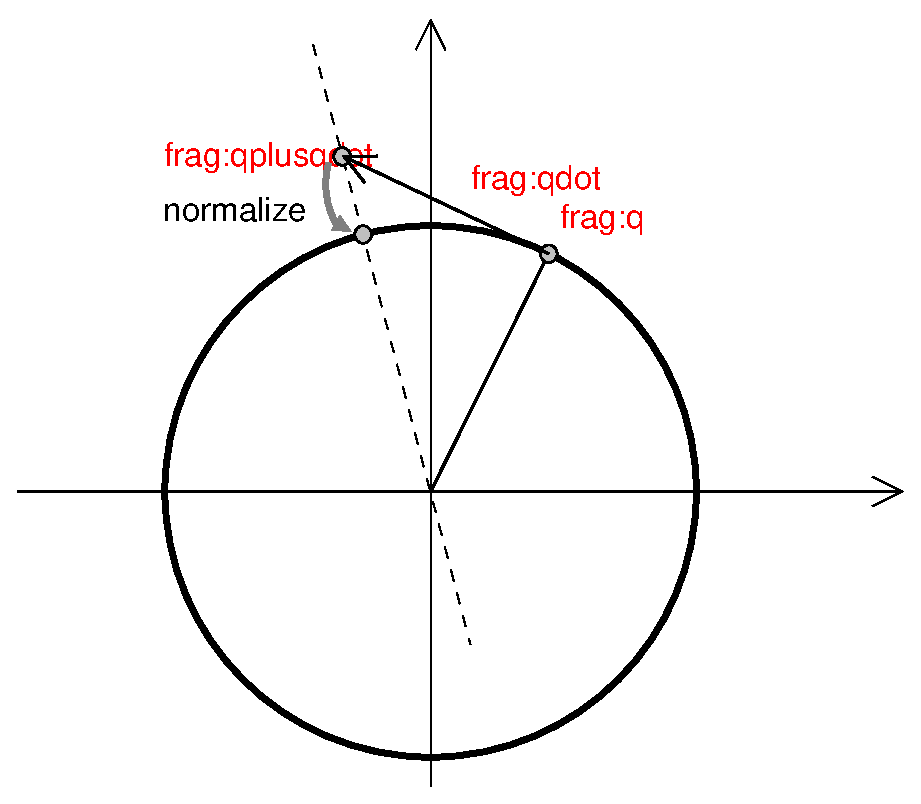
\includegraphics[width=6cm]{figures/quaternion1}}
\caption{Normalizing a quaternion after performing an ODE solving step.
    \label{quatNormalizationFigure}}
\end{figure}

Following the tangent to the sphere is a reasonable approximation to following its curve if the
magnitude of $h \dot{\q{q}}(t)$ is small compared to the curvature of the sphere.
For large time steps or large magnitudes of \ve{\omega}, however, this gets increasingly
erroneous. Consider the limiting case, a body rotating infinitely fast
($\norm{\ve{\omega}} \rightarrow \infty$): after re-normalisation, $\q{q}$ will have moved merely
a quarter of the way around the unit sphere, which equates to concatenating the rotation of
quaternion \q{q} with a rotation by $180^\circ$. This is a strictly finite amount of rotation
per time step, while it would actually have been correct to perform an infinite number of
revolutions around the quaternion sphere.

If a polynomial approximation method like RK4 had been used instead of Euler's method, a
polynomial space curve would have been fitted to the surface of the sphere instead of a straight
line. Note however that the Taylor series of the $\sin$ and $\cos$ functions are nonterminating,
and that it is therefore not possible for a finite polynomial curve to lie exactly in the surface
of a sphere. These ODE solvers will therefore suffer the same problems, albeit less pronounced.


\subsection{Corrected quaternion integration\label{quatIntegrationDerivation}}

Assume that the body we are simulating is rotating at a constant angular velocity.
(This assumption is later weakened by the use of a more sophisticated ODE solver,
but for now we will stick with Euler's method.) Furthermore assume without loss of
generality that the body is rotating clockwise about its $x$ axis, which corresponds
to the world's $x$ axis, and that at time $t=0$ the body's frame and the world frame
coincide. Then the orientation of the body (the quaternion describing
the linear transformation to get from the body's frame of reference into the world
frame) is given as a function of time by
\begin{equation}
\label{quatDerivationExact}
\q{q}(t) = \cos\left(\frac{\norm{\ve{\omega}}t}{2}\right) +
    \sin\left(\frac{\norm{\ve{\omega}}t}{2}\right)\qi
\end{equation}
(cf.\ equation~\ref{quatRotation}, figure~\ref{quatIntFig1}) and its angular velocity is
\begin{equation}
\ve{\omega} = (\omega_1, \omega_2, \omega_3)^T = (\norm{\ve{\omega}}, 0, 0)^T
\end{equation}
for some arbitrary $\norm{\ve{\omega}}$, measured in radians per unit time.

\begin{figure}
\psfrag{frag:omegat}{$\frac{\norm{\ve{\omega}} t}{2}$}
\psfrag{frag:qdotoft}{$\dot{\q{q}}(t)$}
\psfrag{frag:real}{Re}
\psfrag{frag:iimag}{i-Im}
\centerline{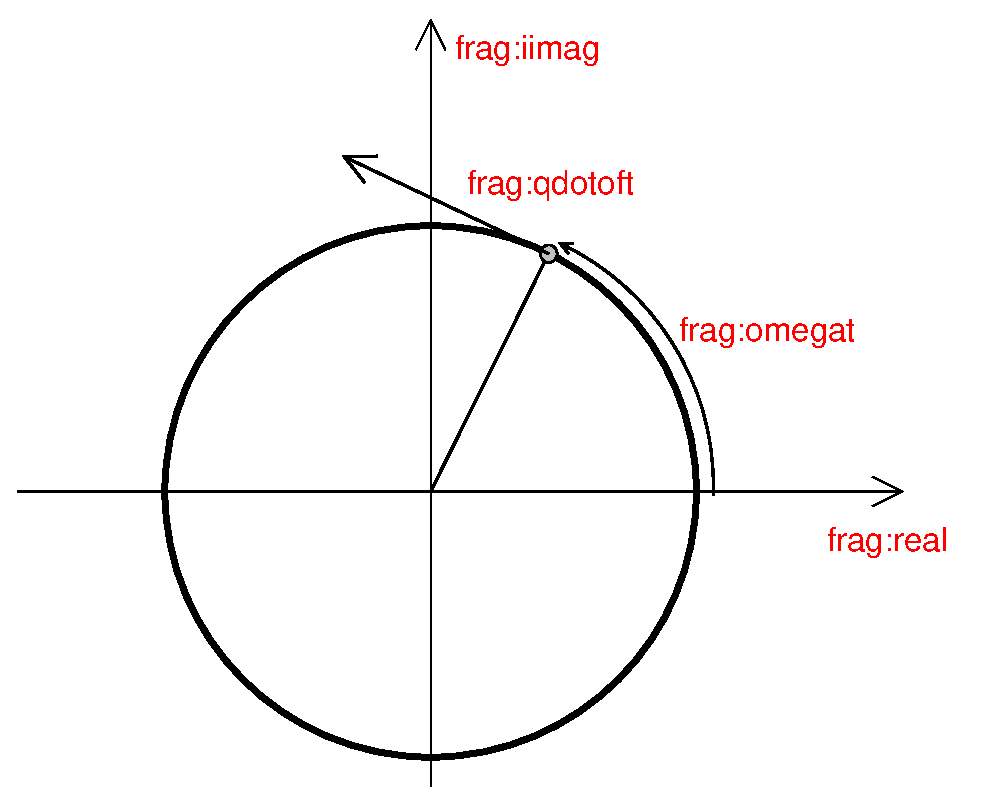
\includegraphics[width=6cm]{figures/quaternion2}}
\caption{Assumed situation for the derivation in
section~\ref{quatIntegrationDerivation}.\label{quatIntFig1}}
\end{figure}

Now assume w.l.o.g.\ that we take a time step from $t = 0$ to $t = h$.
Then we require that the result returned by Euler's method for $\q{q}(h)$
after re-normalization be equal to its exact value in equation~\ref{quatDerivationExact}:
\begin{equation}
\label{quatDerivationSetup}
\cos\left(\frac{\norm{\ve{\omega}} h}{2}\right) +
    \sin\left(\frac{\norm{\ve{\omega}} h}{2}\right)\qi =
    \frac{\q{q}(0) + h \dot{\q{q}}(0)}
        {\norm{\q{q}(0) + h \dot{\q{q}}(0)}}
\end{equation}

We know from examining the 4D geometry that the value assigned to $\dot{\q{q}}$
in equation~\ref{quatRateOfChange} has the correct direction and merely needs to be
corrected in magnitude. In other words, we are searching for a scalar function
$f(h, \norm{\ve{\omega}})$ which will allow $\dot{\q{q}}$ to satisfy
equation~\ref{quatDerivationSetup}:
\begin{equation}
\dot{\q{q}}_h(t) = f\tilde{\ve{\omega}}(t)\q{q}(t)
\end{equation}

Observe that under the above assumptions $\q{q}(0) = 1$, and thus
$\dot{\q{q}}_h(0) = f \norm{\ve{\omega}} \qi$. Substituting this
into equation~\ref{quatDerivationSetup} and considering only the real part:
\begin{eqnarray*}
&& \cos\left(\frac{\norm{\ve{\omega}} h}{2}\right) =
    \left[1 + \left( f \norm{\ve{\omega}} h \right)^2 \right]^{-\frac{1}{2}} \\
&\Leftrightarrow&
    \left( f \norm{\ve{\omega}} h \right)^2 =
    \frac{1}{\cos^2\left(\frac{\norm{\ve{\omega}} h}{2}\right)} - 1 \\
&\Leftrightarrow&
    f(h, \norm{\ve{\omega}}) =
    \frac{1}{\norm{\ve{\omega}} h} \sqrt{\frac{
        1 - \cos^2\left(\frac{\norm{\ve{\omega}} h}{2}\right)}{
        \cos^2\left(\frac{\norm{\ve{\omega}} h}{2}\right)}} =
    \frac{1}{\norm{\ve{\omega}} h}
        \tan\left(\frac{\norm{\ve{\omega}} h}{2}\right)
\end{eqnarray*}

To check, we substitute this result into the $\qi$-imaginary part of
equation~\ref{quatDerivationSetup}:
\begin{eqnarray*}
\sin\left(\frac{\norm{\ve{\omega}} h}{2}\right) & = &
    \tan\left(\frac{\norm{\ve{\omega}} h}{2}\right)
    \left[ 1 + \tan^2\left(\frac{\norm{\ve{\omega}} h}{2}\right)
    \right]^{-\frac{1}{2}} \\
&=& \tan\left(\frac{\norm{\ve{\omega}} h}{2}\right)
    \left[ \frac{\cos^2\left(\frac{\norm{\ve{\omega}} h}{2}\right) +
    \sin^2\left(\frac{\norm{\ve{\omega}} h}{2}\right) }{
    \cos^2\left(\frac{\norm{\ve{\omega}} h}{2}\right) }
    \right]^{-\frac{1}{2}} \\
&=& \tan\left(\frac{\norm{\ve{\omega}} h}{2}\right)
    \cos\left(\frac{\norm{\ve{\omega}} h}{2}\right) \\
&=& \sin\left(\frac{\norm{\ve{\omega}} h}{2}\right)
\end{eqnarray*}

Thus we establish the validity of this expression for $f$. Observe that by using 
L'Hospital's rule, we can find value of $f$ for an infinitesimally small time step:
$$
\lim_{h \to 0} f = \lim_{h \to 0} \frac{ \frac{\norm{\ve{\omega}}}{2}
    \cos^{-2}\left(\frac{\norm{\ve{\omega}} h}{2}\right) }{ \norm{\ve{\omega}} } =
    \frac{1}{2}
$$
i.e.\ we obtain the original equation~\ref{quatRateOfChange} for the
instantaneous rate of change.

Now let $\Delta \q{q} = h \dot{\q{q}} =
    \frac{h}{2} \tilde{\ve{\omega}} \q{q}$.
From equation~\ref{quatRateOfChangeMagnitude} we find that
$\norm{\Delta\q{q}} = \frac{\norm{\ve{\omega}} h}{2}$.
Hence we can simplify the expression for the quaternion correcting factor by expressing it
in terms of $\Delta \q{q}$ as follows:
$$
h f \tilde{\ve{\omega}}\q{q} = \frac{h}{\norm{\ve{\omega}} h}
    \tan\left(\frac{\norm{\ve{\omega}} h}{2}\right) \tilde{\ve{\omega}} \q{q} =
    \tan\left(\norm{\Delta\q{q}}\right) \frac{\Delta\q{q}}{\norm{\Delta\q{q}}}
$$

This expression now has a clear geometric interpretation with respect to the 4D geometry
(see figure~\ref{quatIntFig2}):
$\norm{\Delta\q{q}}$ is measured in radians, and it corresponds to the \emph{correct}
angle between the old and the new vector $\q{q}$. Since $\q{q}$ and
$\dot{\q{q}}$ are orthogonal, we have a right-angled triangle between the origin,
the old and the new points $\q{q}$, and hence we can use the $\tan$ function to
evaluate the required length of the side in direction $\Delta\q{q}$.

\begin{figure}
\psfrag{frag:real}{Re}
\psfrag{frag:iimag}{i-Im}
\psfrag{frag:q}{\q{q}}
\psfrag{frag:deltaq}{$\Delta\q{q}$}
\psfrag{frag:quergs1}{$\q{q}+\tan(\norm{\Delta\q{q}})\frac{\Delta\q{q}}{\norm{\Delta\q{q}}}$}
\psfrag{frag:quergs2}{$\mathrm{Quergs}(\q{q},\,\Delta\q{q})$}
\centerline{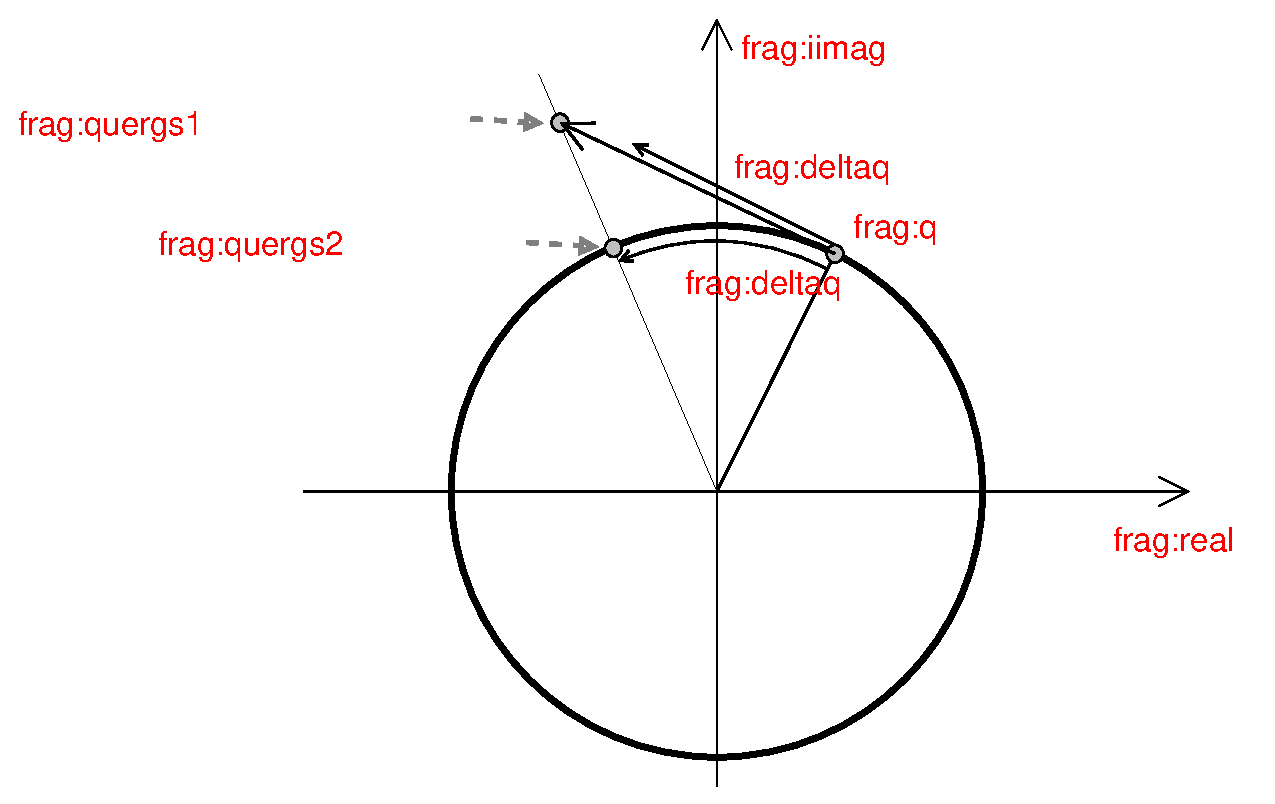
\includegraphics[width=7.7cm]{figures/quaternion3}}
\caption{Illustration of the operation of Quergs.\label{quatIntFig2}}
\end{figure}

Finally we can combine this correction and the subsequent quaternion normalisation into
a single function:
\begin{eqnarray*}
\q{q}(t+h) = \mathrm{Quergs}(\q{q}(t), \Delta\q{q}) &=&
    \frac{\q{q}(t) + \tan\left(\norm{\Delta\q{q}}\right)
        \frac{\Delta\q{q}}{\norm{\Delta\q{q}}}}{
    \norm{\q{q}(t) + \tan\left(\norm{\Delta\q{q}}\right)
        \frac{\Delta\q{q}}{\norm{\Delta\q{q}}}}} \\
&=& \frac{\q{q}(t) + \tan\left(\norm{\Delta\q{q}}\right)
        \frac{\Delta\q{q}}{\norm{\Delta\q{q}}}}{
    \sqrt{1 + \tan^2\left(\norm{\Delta\q{q}}\right)}} \\
&=& \left[\q{q}(t) + \tan\left(\norm{\Delta\q{q}}\right)
        \frac{\Delta\q{q}}{\norm{\Delta\q{q}}}\right]
    \cos\left(\norm{\Delta\q{q}}\right)
\end{eqnarray*}
The last expression is simplest (and again allows geometric interpretation), but probably
the first of the three expressions is more useful for numerical evaluation, since it involves
only one trigonometric function and minimizes numerical errors.

When implementing this formula, care must be taken around the discontinuities of the $\tan$
function, where numerical instability may occur. These discontinuities are reached whenever a
body performs an odd multiple of half revolutions during a single time step.


\subsection{Applying Quergs to Runge-Kutta\label{quergsRK4}}

Quergs implements one step of Euler's method for solving an ODE over a quaternion.
Where for Euler's method over an Euclidean vector we would write
$\ve{a}(t + h) = \ve{a}(t) + h\,\dot{\ve{a}}(t,\;\ve{a}(t))$,
for quaternions we simply use
$\q{q}(t + h) = \mathrm{Quergs}(\q{q}(t),\; h\,\dot{\q{q}}(t)) =
    \mathrm{Quergs}(\q{q}(t),\; \frac{h}{2}\,\tilde{\ve{\omega}}(t)\q{q}(t))$.

We can apply Quergs to polynomial ODE solvers by following the same pattern: wherever the solver
computes the sum of a quantity and a delta of that quantity (a delta being a derivative
scaled with the time step size and other factors), we substitute Quergs in place of that
addition. Assume we have a function $\dot{\q{q}}(t,\; \q{q}(t))$ which computes the
instantaneous rate of change at time $t$, given the state $\q{q}(t)$ at that time. Then we can
define the formulae for the fourth-order Runge-Kutta solver (RK4, based on the definition
in~\cite{NRinC}) over quaternions as follows:
\begin{eqnarray}
\Delta\q{q}_1 & = & h\;\dot{\q{q}}\left(t,\;\q{q}(t)\right) \nonumber\\
\Delta\q{q}_2 & = & h\;\dot{\q{q}}\left(t + \frac{h}{2},\;
    \mathrm{Quergs}\left(\q{q}(t),\; \frac{1}{2}\Delta\q{q}_1\right)\right) \nonumber\\
\Delta\q{q}_3 & = & h\;\dot{\q{q}}\left(t + \frac{h}{2},\;
    \mathrm{Quergs}\left(\q{q}(t),\; \frac{1}{2}\Delta\q{q}_2\right)\right) \nonumber\\
\Delta\q{q}_4 & = & h\;\dot{\q{q}}\left(t + h,\;
    \mathrm{Quergs}\left(\q{q}(t),\; \Delta\q{q}_3\right)\right) \nonumber\\
\q{q}(t + h) & = & \mathrm{Quergs}\left(\q{q}(t),\;
    \frac{1}{6}\Delta\q{q}_1 + \frac{1}{3}\Delta\q{q}_2 +
    \frac{1}{3}\Delta\q{q}_3 + \frac{1}{6}\Delta\q{q}_4\right)
\end{eqnarray}

Why is it correct to compute the weighted sum over $\Delta\q{q}_1$ to
$\Delta\q{q}_4$ in the last formula, when we have replaced all other quaternion additions
by calls to Quergs? Remember that finite movements on the quaternion hypersphere are
equivalent to rotations in 4D, and that these are not commutative. Differential
rotations are, however, commutative~-- like in 3D. (This is the reason why we can
use component-by-component integration to determine angular momentum:
like angular velocity, it is a differential of rotation.) Here, $\Delta\q{q}_1$ to
$\Delta\q{q}_4$ are also weighted differentials, and therefore subject to
conventional summation. Finally observe that each of $\Delta\q{q}_1$ to
$\Delta\q{q}_4$ is orthogonal to \q{q} (appendix~\ref{quatIntegrationMagnitude}),
and that therefore the weighted sum of all of these, expressed as a vector, also
lies in the hyperplane which is tangential to the unit sphere at the point \q{q},
and is therefore a valid derivative.

\section{Free precession\label{correctBrettAppendix}}

This argument is modelled after~\cite{Ruf:02}. The moment of inertia $\ve{L}$ of a rigid
body is defined as
\begin{equation}
\label{correctBrett1}
\ve{L} = \m{I}\ve{\omega}
\end{equation}
where $\m{I}$ is the inertia tensor and $\ve{\omega}$ is the angular velocity vector.
Torque is the rate of change of angular momentum over time:
\begin{equation}
\label{correctBrett2}
\ve{\tau} = \dot{\ve{L}} = \dot{\m{I}}\ve{\omega} + \m{I}\dot{\ve{\omega}}
\end{equation}

We can further evaluate $\dot{\m{I}}$ by writing \m{I} as a product with some rotation matrix
$\m{R}$ and its transpose:
\begin{equation}
\label{correctBrett3}
\m{I} = \m{R}\m{I}_\mathrm{body}\m{R}^T
\end{equation}

It can be shown that such a decomposition of the inertia tensor always exists, and that
$\m{I}_\mathrm{body}$ is a diagonal, time-invariant matrix containing the moments
of inertia about the body's principal axes~\cite{Feynman:63}. Hence we obtain
\begin{equation}
\label{correctBrett4}
\dot{\m{I}} = \dot{\m{R}}\m{I}_\mathrm{body}\m{R}^T +
    \m{R}\m{I}_\mathrm{body}\frac{\diff}{\diff t}\m{R}^T
\end{equation}

Witkin~\cite{BaraffWitkin:97} derives that $\dot{\m{R}} = \dual{\ve{\omega}}\,\m{R}$
for a rotation matrix $\m{R}$ and an angular velocity vector $\ve{\omega}$.
Using this identity and taking the differential operator onto the inside of the
transpose at the end of equation~\ref{correctBrett4},
\begin{eqnarray}
\dot{\m{I}} &=& \dual{\ve{\omega}}\,\m{R}\m{I}_\mathrm{body}\m{R}^T +
    \m{R}\m{I}_\mathrm{body}(\dual{\ve{\omega}}\,\m{R})^T \nonumber\\
&=& \dual{\ve{\omega}}\,\m{R}\m{I}_\mathrm{body}\m{R}^T -
    \m{R}\m{I}_\mathrm{body}\m{R}^T\dual{\ve{\omega}} \nonumber\\
&=& \dual{\ve{\omega}}\,\m{I} - \m{I}\dual{\ve{\omega}} \label{correctBrett5}
\end{eqnarray}

Substituting equation~\ref{correctBrett5} back into~\ref{correctBrett2}:
\begin{eqnarray}
\ve{\tau} & = & \m{I}\dot{\ve{\omega}} + \dual{\ve{\omega}}\,\m{I}\ve{\omega} -
    \m{I}\dual{\ve{\omega}}\,\ve{\omega} \nonumber \\
& = & \m{I}\dot{\ve{\omega}} + \dual{\ve{\omega}}\,\m{I}\ve{\omega} \label{correctBrett6}
\end{eqnarray}

Equation~\ref{correctBrett6} corrects the similar expression in~\cite{Saunders:PhD},
page~34. This means that the angular acceleration of a rigid body is given by
\begin{equation}
\label{correctBrett7}
\dot{\ve{\omega}} = \m{I}^{-1} (\ve{\tau} - \dual{\ve{\omega}}\,\m{I}\ve{\omega}).
\end{equation}
where \ve{\tau} is the sum of all torque vectors acting on the body. This means that even if
there are no torques, its angular velocity may change if \m{I} is not diagonal (i.e.\ if
the body is somehow asymmetric). This effect is called \emph{free precession}.

In a simulation, we usually integrate over torques to find angular momentum, and then calculate
the angular velocity from the momentum in each time step using the current moment of inertia. In
this case, the angular acceleration in equation~\ref{correctBrett7} is not needed. It is required
only for purposes of computing constraint forces and torques.

\section{Constrained rigid body dynamics}
The methods we have developed so far allow the simulation of a single rigid body with forces
acting on it. Further challenges arise when we consider multibody systems in which the bodies
interact in some way. We will primarily be interested in articulated bodies, that is, systems
of individual rigid bodies held together by joints. Joints allow rotation but cannot be
separated. (The human body is a good example of such an articulated body.)

There are various strategies for implementing articulated bodies. {\em Lagrangian mechanics}
is a commonplace method in physics and engineering, in which the state of the system is expressed
in terms of a set of {\em generalised coordinates}. The position and orientation of each sub-body
is then a function of these generalised coordinates, and outside forces can be transformed
back into the generalised coordinates, where they are handled. For example, consider two rigid
bodies which are held together by a ball-and-socket joint~\cite{Kalra:95}. Without the joint,
the system would have 12 degrees of freedom at rest: three translational and three rotational
degrees for each of the bodies. In a Lagrangian formulation, the two connected bodies would be
expressed in nine coordinates: six for translation and rotation of the first body, and three
for the rotation of the second body with respect to the first.

Lagrangian mechanics has the advantage that if formulated correctly, the system will always in a
legal state, no matter what the values of the coordinates are. It also allows very fast
computation. On the downside, the functions to transform the coordinates become very hard or
impossible to find for complicated systems, so the method does not scale well.

An alternative approach to the problem is to initially grant each sub-body its full number of
degrees of freedom, and then to impose constraints on the system. We can then ensure that the
constraints are always maintained by excerting appropriate forces and torques on the bodies.
Finding these forces is commonly done by means of {\em Lagrange multipliers}~-- note that
despite the similarity in name, this method has very little in common with Lagrangian mechanics.

Lagrange multipliers are used to implement constrained rigid body mechanics in this project,
because once set up, such a system can handle a large variety of situations with ease.
The mathematical formulation of Lagrange multipliers is derived in~\cite{BaraffWitkin:97} and
extended in~\cite{Saunders:PhD} (also see~\cite{Baraff:96} for an optimized algorithm),
therefore we only state the results here.

Consider a system of $n$ rigid bodies at a particular point in time. Each body has a vector
pointing to its centre of mass, and an orientation. Assume that we can concatenate these
parameters of all bodies into a global state vector\footnote{Witkin calls this vector
$\ve{q}$; we use $\ve{x}$ here to avoid confusion with quaternions.} $\ve{x}$.
Containing a value for each degree of freedom, $\ve{x}$ will have $6n$ rows. In practice
we will never need to write down $\ve{x}$ explicitly; instead we will work with its
first and second derivative in time, $\dot{\ve{x}}$ and $\ddot{\ve{x}}$ respectively.

For example, in a system with two bodies, having centre of mass positions $\ve{a}$ and
$\ve{b}$, and angular velocities $\ve{\omega}$ and $\ve{\phi}$ respectively, we would
have
\begin{equation}
\label{lagrangeStateVector}
\dot{\ve{x}} = \left[ \begin{array}{c}
    \dot{\ve{a}}\\ \ve{\omega}\\ \dot{\ve{b}}\\ \ve{\phi} \end{array}\right]
\quad\quad\mathrm{and}\quad\quad
\ddot{\ve{x}} = \left[ \begin{array}{c}
    \ddot{\ve{a}}\\ \dot{\ve{\omega}}\\ \ddot{\ve{b}}\\ \dot{\ve{\phi}} \end{array}\right]
\end{equation}

Now assume that we want to impose $m$ constraints on this system, where each constraint
effectively reduces the number of degrees of freedom by one. (A constraint specifying a
ball-and-socket joint, as described earlier, would therefore have to be expressed as a
vector of three constraints.) Express each constraint as a function $c$ which is zero
when the constraint is satisfied. We can then combine all constraint functions into a
single $m$-row constraint vector $\ve{c}$. Each valid configuration of the system must
satisfy $\ve{c} = \ve{0}$, the null vector.

To find the constraint maintaining forces, we must know how a change in state or a change in
time affects the value of $\ve{c}$. To this end, we must calculate the first two partial
derivatives of $\ve{c}$ with respect to time, $\dot{\ve{c}}$ and $\ddot{\ve{c}}$.
We also calculate the Jacobian matrix~\cite{RHB:02} $\m{J}$ which contains all partial
derivatives of $\ve{c}$ w.r.t. all coordinates of $\ve{c}$, and the similarly
defined Jacobian $\dot{\m{J}}$ of $\dot{\ve{c}}$:
\begin{equation}
J_{ij} = \frac{\partial c_i}{\partial x_j} \quad\quad\mathrm{and}\quad\quad
\dot{J}_{ij} = \frac{\partial \dot{c}_i}{\partial x_j}
\end{equation}

Both $\m{J}$ and $\dot{\m{J}}$ are $6n\times m$ matrices. However, since we do not
have an explicit expression for $\ve{x}$, we cannot calculate them directly using
partial differentiation. Instead we make use of the following results of the chain rule:
\begin{equation}
\label{cDotAndCDDot}
\dot{\ve{c}} = \m{J}\dot{\ve{x}} \quad\quad\mathrm{and}\quad\quad
\ddot{\ve{c}} = \dot{\m{J}}\dot{\ve{x}} + \m{J}\ddot{\ve{x}}.
\end{equation}
Appendix~\ref{constraintAppendix} gives examples of derivations using these equations.

Two more quantities are required before we can determine the forces and torques which maintain
our constraints. We need to add up all the other forces and torques acting on each of the $n$
sub-bodies (for example due to gravity or muscular activity) and concatenate them into a single
$6n$-row vector \ve{\Phi}, just as we did for \ve{x}. Re-using the two-body case of
equation~\ref{lagrangeStateVector}:
\begin{equation}
\ve{\Phi} = \left[\begin{array}{l}
    \sum \ve{F}_A \\
    \left( \sum \ve{\tau}_A \right) - \ve{\omega}\times(\m{I}_A\,\ve{\omega}) \\
    \sum \ve{F}_B \\
    \left( \sum \ve{\tau}_B \right) - \ve{\phi}\times(\m{I}_B\,\ve{\phi})
    \end{array}\right]
\end{equation}
where $\ve{F}_A$ denotes a force vector acting on the centre of mass of body~A, $\ve{\tau}_A$
is a torque vector acting on body~A, and $\m{I}_A$
the moment of inertia of body~A in the world frame. The expression
$\ve{\omega}\times(\m{I}_A\,\ve{\omega})$ and its analogue for the other bodies do
not strictly represent torques, but subtracting them here ensures that angular momentum is
conserved in the absence of other torques. See appendix~\ref{correctBrettAppendix} for the
derivation of this expression.

And finally, we require the {\em mass-inertia tensor} \m{M} and its inverse
$\m{M}^{-1}$. Both are $6n\times6n$ matrices of the form
\begin{equation}
\label{massInertiaTensor}
\m{M} = \left[ \begin{array}{ccccccc}
    \mu_1\m{1} \\ & \m{I}_1 \\ &&
    \mu_2\m{1} \\ &&& \m{I}_2 \\ &&&& \ddots \\ &&&&&
    \mu_n\m{1} \\ &&&&&& \m{I}_n
    \end{array}\right]
\end{equation}

Here $\mu_i$ denotes the (scalar) mass of body $i$, \m{1} stands for the $3\times3$
identity matrix, and $\m{I}_i$ is the inertia tensor (written as a $3\times3$ matrix)
of body $i$ in the world frame. All empty regions are zero. While $\mu_i$ will typically
stay constant over time, $\m{I}_i$ may depend on the orientation of body $i$.\footnote{If
we know the principal axes of the body, we can express \m{I} in a time-invariant
form combined with rotations into the principal axes frame and back again
(see~\cite{BaraffWitkin:97}), which saves us a lot of effort.} The inverse $\m{M}^{-1}$
is obtained by replacing each $\mu$ by $\frac{1}{\mu}$ and each $\m{I}$ by
$\m{I}^{-1}$ in equation~\ref{massInertiaTensor}.

Now we can set up the equation\footnote{Here we adopt the sign convention
of~\cite{BaraffWitkin:97}, which is the opposite of~\cite{Saunders:PhD}.}
\begin{equation}
\label{lagrangeEquation}
-\m{J}\m{M}^{-1}\m{J}^T\ve{\lambda} = \dot{\m{J}}\dot{\ve{x}} +
    \m{J}\m{M}^{-1}\ve{\Phi} + k\ve{c} + d\dot{\ve{c}}
\end{equation}
in which all variables except $\ve{\lambda}$ are known. The meaning of this equation and
its two scalar constants $k$ and $d$ is discussed in~\cite{BaraffWitkin:97}
and~\cite{Saunders:PhD}. For us it will suffice to consider it to be a `black box' which can be
given to a linear equation solver to obtain $\ve{\lambda}$.

$\ve{\lambda}$ is an $m$-row vector of so-called Lagrange multipliers (after which this method
is named), where $m$ is the number of constraints. Once we have solved for it, we can compute
the expression
\begin{equation}
\hat{\ve{\Phi}} = \m{J}^T\,\ve{\lambda}.
\end{equation}
$\hat{\ve{\Phi}}$ has the same format as $\ve{\Phi}$, and indeed it is the vector containing
the forces and torques which we need to additionally apply to each body to ensure that they
continue to satisfy the constraints! The bodies' constrained movements are calculated by
the generalised form of the familiar formula $\ddot{x} = \frac{F}{m}$:
\begin{equation}
\ddot{\ve{x}} = \m{M}^{-1}\,(\ve{\Phi} + \hat{\ve{\Phi}})
\end{equation}
This result, $\ddot{\ve{x}}$, can now be fed directly into our ODE solver.

\section{A catalog of constraint functions\label{constraintAppendix}}

Let us consider some examples of constraints to clarify the procedure.

\subsection{Fixed point in space (`Nail')}

Let us implement a constraint which `nails' a particular point in a rigid body to a fixed point
in world space. (It's a very flexible nail, because despite fixing the position, it allows all
three modes of rotation.) Let \ve{p} be the position of the centre of mass of our rigid
body, \ve{s} the vector from the centre of mass to the point in the body we want to attach,
$\ve{\omega}$ the angular velocity of the rigid body, and \ve{t} the coordinates in world
space that we want to nail the point to. Then we can set up a very simple constraint function,
\begin{equation}
\ve{c} = \ve{p} + \ve{s} - \ve{t}
\end{equation}
which equals the null vector when $\ve{p}+\ve{s}$ and $\ve{t}$ coincide, as required.
Since this is a three-dimensional vector equation, we are actually defining three constraints
at once. Since \ve{t} does not change over time, we obtain
\begin{eqnarray}
\dot{\ve{c}} &=& \dot{\ve{p}} + \ve{\omega}\times\ve{s} \nonumber\\
&=& \dot{\ve{p}} - \dual{\ve{s}}\,\ve{\omega} \\
\ddot{\ve{c}} &=& \ddot{\ve{p}} + \dot{\ve{\omega}}\times\ve{s} +
    \ve{\omega}\times(\ve{\omega}\times\ve{s}) \nonumber\\
&=& \ddot{\ve{p}} - \dual{\ve{s}}\,\dot{\ve{\omega}} -
    \dual{(\ve{\omega}\times\ve{s})}\,\ve{\omega}
\end{eqnarray}
(cf. similar derivations in~\cite{Kalra:95}). We have already moved the `chosen variables' to
the rightmost position of each product. We will now factor $\dot{\ve{c}}$ and write out the
components of $\m{J}$ in terms of the vector components:

\begin{equation}
\label{constrEx1J}
\dot{\ve{c}} = \left[\begin{array}{ccc} 1&0&0\\0&1&0\\0&0&1 \end{array}\right]
    \dot{\ve{p}} + \left[\begin{array}{ccc}
    0 & s_3 & -s_2 \\ -s_3 & 0 & s_1 \\ s_2 & -s_1 & 0
    \end{array}\right] \ve{\omega}
\end{equation}

The two matrices in equation~\ref{constrEx1J} thus form two slices of $\m{J}$ at
the locations appropriate for $\dot{\ve{p}}$ and $\ve{\omega}$. We now continue to the
next step of the procedure:

\begin{eqnarray}
\dot{\m{J}}\dot{\ve{x}} = 
\ddot{\ve{c}} - \m{J}\ddot{\ve{x}} &=&
    \big(\ddot{\ve{p}} - \dual{\ve{s}}\,\dot{\ve{\omega}} -
    \dual{(\ve{\omega}\times\ve{s})}\,\ve{\omega}\big) -
    (\ddot{\ve{p}} - \dual{\ve{s}}\,\dot{\ve{\omega}}) \nonumber\\
& = & -\dual{(\ve{\omega}\times\ve{s})}\,\ve{\omega} \nonumber\\
& = & \left[\begin{array}{ccc} 0 &
    \omega_1 s_2 - \omega_2 s_1 &
    \omega_1 s_3 - \omega_3 s_1 \\
    \omega_2 s_1 - \omega_1 s_2 & 0 &
    \omega_2 s_3 - \omega_3 s_2 \\
    \omega_3 s_1 - \omega_1 s_3 &
    \omega_3 s_2 - \omega_2 s_3 & 0
    \end{array}\right] \ve{\omega} \nonumber\\\label{constrEx1JDot}
\end{eqnarray}

We see that here there is only one slice for $\dot{\m{J}}$; the rest of the matrix
is zero. Since $\ve{\omega}$ also occurs inside the matrix, there are actually several
alternative representations of this matrix which are equally valid.

\subsection{Ball-and-socket joint}

Two rigid bodies are attached together at a particular point in each of the bodies.
They may not separate, but all three rotational degrees of freedom are permitted. This is
a good representation e.g. of a human shoulder joint.

Let $\ve{a}$ and $\ve{b}$ be the positions of the centres of mass in the first and
second rigid body respectively. Let $\ve{s}$ be the vector from $\ve{a}$ to the 
attachment point, and $\ve{t}$ the vector from $\ve{b}$ to the attachment point.
Also let $\ve{\omega}$ be the angular velocity of the first body, and $\ve{\phi}$ that
of the second. Then our constraint function and its derivatives are:

\begin{eqnarray}
\ve{c} &=& \ve{a} + \ve{s} - \ve{b} - \ve{t} \\
\dot{\ve{c}} &=& \dot{\ve{a}} + \ve{\omega}\times\ve{s} -
    \dot{\ve{b}} - \ve{\phi}\times\ve{t} \\
\ddot{\ve{c}} &=& \ddot{\ve{a}} + \dot{\ve{\omega}}\times\ve{s} +
    \ve{\omega}\times(\ve{\omega}\times\ve{s}) -
    \ddot{\ve{b}} - \dot{\ve{\phi}}\times\ve{t} -
    \ve{\phi}\times(\ve{\phi}\times\ve{t})
\end{eqnarray}

The rest of the derivation is very similar to the previous example. We obtain four
matrix slices for \m{J} and two slices for $\dot{\m{J}}$.


\subsection{Rotation axis restriction (`Joystick')}

We now have formulae to define a ball-and-socket joint. How can we express other types
of joints? A good way of doing this is by augmenting the ball-and-socket constraint with
additional constraints which restrict the set of valid rotations. In this section we will
derive expressions for a constraint which prohibits rotation about one particular axis~--
or, in other words, confines the axis to a plane. Let us define a unit vector \ve{n} which
points in the direction of the axis we want to prohibit; equivalently, this is the normal of
the confinement plane.

It is not completely easy to visualize what this type of constraint means. One good way to look
at it is to consider a standard two-axis joystick. If it is placed on a table, the two axes of
rotation lie in a plane parallel to the surface of this table. But you cannot turn the stick about
its own axis. Hence the normal of the constraint plane is orthogonal to the table surface.
Don't be confused by the fact that the joystick handle happens to point in the direction of the
normal~-- any sort of obscure shape may be substituted in its place without changing the nature
of the constraint!

A more common sort of joint is the hinge, which we find in most doors, in our knees and elbows.
It allows rotation only about one particular axis. We can conveniently express it by employing two
`joystick' constraints on the same body, each of which confines the axis to a plane. Provided the
two planes are not parallel, the axis about which rotation may occur corresponds to the line of
intersection of these two planes. In summary, to make a hinge joint, we first add a
ball-and-socket joint. Then we find two non-colinear vectors which are both orthogonal to the
hinge axis, and use them as normal vectors for two `joystick' constraints. This reduces the
original number of six degrees of freedom to one~-- the angle of the hinge.

We shall now consider the relative rotation of two rigid bodies. Say the first body has an
orientation quaternion \q{p} and angular velocity \ve{\phi}, and the second body orientation
\q{q} and angular velocity \ve{\omega}. Assume that each quaternion expresses the rotation
required to transform from the body's frame to the world frame. Then the quaternion product
$\q{p}^{-1}\q{q}$ is the rotation required to transform from the second body's frame to the first
one's~-- that is, the relative rotation of the two bodies.

To confine the axis of rotation, we use the fact that the axis is contained in the imaginary
parts of a quaternion (equation~\ref{quatRotation}, page~\pageref{quatRotation}). We want the dot
product of this axis and the normal vector \ve{n} to be zero. Conveniently, the dot product
happens to be implicitly present in the real part of the quaternion product
(equation~\ref{quatProduct2}, page~\pageref{quatProduct2}). Hence we can define our constraint
function as follows:
\begin{equation}
\ve{c} = \Re(\tilde{\ve{n}}\, \q{p}^{-1}\q{q})
\end{equation}

As with complex numbers, the function $\Re$ returns only the real part of its argument.
Since the real part of $\tilde{\ve{n}}$ is zero by definition, this is just the dot product of
\ve{n} and the axis of $\q{p}^{-1}\q{q}$, with an extra minus sign in front~(cf.
equation~\ref{quatProduct2}). The constraint function is actually a scalar because we are only
losing one degree of freedom, but for consistency's sake, we will write it as a one-component
vector.

The derivative of \q{q} with respect to time is
$\dot{\q{q}} = \frac{1}{2}\tilde{\ve{\omega}}\q{q}$, as usual. Pushing the differential operator
onto the inside of a quaternion inverse produces a minus sign and reverses the order, provided
we are dealing with a unit quaternion:
\begin{equation}
\frac{\diff}{\diff t} \q{p} = \frac{1}{2}\tilde{\ve{\phi}}\,\q{p} \iff
    \frac{\diff}{\diff t} (\q{p}^{-1}) = -\frac{1}{2}\q{p}\,\tilde{\ve{\phi}}
\end{equation}

We now have everything in place to calculate the constraint function derivatives:
\begin{eqnarray}
\dot{\ve{c}} & = & \label{constrJoystickC}
    \frac{1}{2} \Re(\tilde{\ve{n}}\, \q{p}^{-1}\, \tilde{\ve{\omega}}\,\q{q}) -
    \frac{1}{2} \Re(\tilde{\ve{n}}\, \q{p}^{-1}\, \tilde{\ve{\phi}}\, \q{q}) \\
\ddot{\ve{c}} & = & \label{constrJoystickCDot}
    \frac{1}{2} \Re(\tilde{\ve{n}}\, \q{p}^{-1}\, \tilde{\dot{\ve{\omega}}}\,\q{q})
  - \frac{1}{2} \Re(\tilde{\ve{n}}\, \q{p}^{-1}\, \tilde{\dot{\ve{\phi}}}\, \q{q}) \\*
&&+ \frac{1}{4} \Re(\tilde{\ve{n}}\, \q{p}^{-1}\, \tilde{\ve{\omega}}\,\tilde{\ve{\omega}}\, \q{q})
  - \frac{1}{2} \Re(\tilde{\ve{n}}\, \q{p}^{-1}\, \tilde{\ve{\phi}}\,\tilde{\ve{\omega}}\, \q{q})
  + \frac{1}{4} \Re(\tilde{\ve{n}}\, \q{p}^{-1}\, \tilde{\ve{\phi}}\,\tilde{\ve{\phi}}\, \q{q})
    \nonumber
\end{eqnarray}

To manipulate these equations into the form required to find \m{J} we use the scalar/vector
pair notation for quaternions~-- see page~\pageref{quatProduct2}.
\begin{eqnarray*}
\Re(\tilde{\ve{n}}\, \q{p}^{-1}\, \tilde{\ve{\omega}}\,\q{q}) & = &
    \Re\big( [0,\:\ve{n}]\: [p_w,\:-\ve{p}_v]\: [0,\:\ve{\omega}]\: [q_w,\:\ve{q}_v] \big) \\*
&=& \Re\big( [\ve{n}\cdot\ve{p}_v,\: p_w\ve{n} - \ve{n}\times\ve{p}_v]\:
             [-\ve{\omega}\cdot\ve{q}_v,\: q_w\ve{\omega} + \ve{\omega}\times\ve{q}_v] \big) \\*
&=& -(\ve{n}\cdot\ve{p}_v) (\ve{\omega}\cdot\ve{q}_v) -
    ( p_w\ve{n} - \ve{n}\times\ve{p}_v ) \cdot ( q_w\ve{\omega} + \ve{\omega}\times\ve{q}_v ) \\*
&=& -\ve{n}^T \ve{p}_v \ve{q}_v^T \ve{\omega} - ( p_w\ve{n} + \ve{p}_v\times\ve{n} )^T
    ( q_w\ve{\omega} - \ve{q}_v\times\ve{\omega} ) \\*
&=& -\ve{n}^T \ve{p}_v \ve{q}_v^T \ve{\omega} - ( p_w\ve{n}^T - \ve{n}^T\dual{\ve{p}_v} )
    ( q_w\ve{\omega} - \dual{\ve{q}_v}\,\ve{\omega} ) \\*
&=& -\ve{n}^T \big( \ve{p}_v \ve{q}_v^T + ( p_w\m{1} - \dual{\ve{p}_v} )
    ( q_w\m{1} - \dual{\ve{q}_v} ) \big)\, \ve{\omega}
\end{eqnarray*}

Here \m{1} denotes the $3\times3$ identity matrix. The same derivation is valid if we substitute
\ve{\phi} for \ve{\omega}, hence we obtain the Jacobian
\begin{eqnarray}
\m{J}\dot{\ve{x}} & = & 
    -\frac{1}{2} \ve{n}^T \big( \ve{p}_v \ve{q}_v^T + ( p_w\m{1} - \dual{\ve{p}_v} )
    ( q_w\m{1} - \dual{\ve{q}_v} ) \big)\, \ve{\omega} \nonumber\\*
&&  +\frac{1}{2} \ve{n}^T \big( \ve{p}_v \ve{q}_v^T + ( p_w\m{1} - \dual{\ve{p}_v} )
    ( q_w\m{1} - \dual{\ve{q}_v} ) \big)\, \ve{\phi}
\end{eqnarray}

Now the first two terms of equation~\ref{constrJoystickCDot} are generated by $\m{J}\ddot{x}$, so
for finding $\dot{\m{J}}$ we need only consider the last three terms. Let's evaluate the
penultimate term (take a deep breath):
\begin{eqnarray*}
\Re(\tilde{\ve{n}}\, \q{p}^{-1}\, \tilde{\ve{\phi}}\,\tilde{\ve{\omega}}\, \q{q}) & = &
    \Re\big( [0,\:\ve{n}]\: [p_w,\:-\ve{p}_v]\: [0,\:\ve{\phi}]\: [0,\:\ve{\omega}]\:
    [q_w,\:\ve{q}_v] \big) \\*
&=& \Re\big( [0,\:\ve{n}]\: [\ve{p}_v \cdot \ve{\phi},\: p_w\ve{\phi} - \ve{p}_v\times\ve{\phi}]\:
    [-\ve{\omega}\cdot\ve{q}_v,\: q_w\ve{\omega} + \ve{\omega}\times\ve{q}_v] \big) \\*
&=& \Re\Big( \begin{array}[t]{lll} \big[ &
    \ve{n}\cdot(\ve{p}_v\times\ve{\phi}) - p_w \ve{\phi}\cdot\ve{n}, &\\ &
    (\ve{p}_v\cdot\ve{\phi}) \ve{n} + p_w\ve{n}\times\ve{\phi} -
        \ve{n}\times(\ve{p}_v\times\ve{\phi}) \quad\big] &\\
    \big[ & -\ve{\omega}\cdot\ve{q}_v,\: q_w\ve{\omega} +
        \ve{\omega}\times\ve{q}_v \quad\big] & \Big) \end{array} \\
&=& -\big( \ve{n}\cdot(\ve{p}_v\times\ve{\phi}) - p_w \ve{\phi}\cdot\ve{n} \big)
     \big( \ve{\omega}\cdot\ve{q}_v \big) \\* &&
    -\big( (\ve{p}_v\cdot\ve{\phi}) \ve{n} + p_w\ve{n}\times\ve{\phi} -
        \ve{n}\times(\ve{p}_v\times\ve{\phi}) \big) \cdot
     \big( q_w\ve{\omega} - \ve{q}_v\times\ve{\omega} \big) \\
&=& -\big( \ve{n}\cdot(\ve{p}_v\times\ve{\phi}) \big) \big( \ve{q}_v\cdot\ve{\omega} \big)
    + p_w (\ve{n}\cdot\ve{\phi}) (\ve{q}_v\cdot\ve{\omega}) \\* &&
    +\big( \ve{n}\cdot(\ve{q}_v\times\ve{\omega}) \big) \big( \ve{p}_v\cdot\ve{\phi} \big)
    - q_w (\ve{n}\cdot\ve{\omega}) (\ve{p}_v\cdot\ve{\phi}) \\* &&
    -\big( \ve{n}\times(p_w\ve{\phi} - \ve{p}_v\times\ve{\phi}) \big) \cdot
     \big( q_w\ve{\omega} - \ve{q}_v\times\ve{\omega} \big) \\
&=&  \ve{n}^T (p_w\m{1} - \dual{\ve{p}_v})\, \ve{\phi}\,\ve{q}_v^T \ve{\omega}
    -\ve{n}^T (q_w\m{1} - \dual{\ve{q}_v})\, \ve{\omega}\,\ve{p}_v^T \ve{\phi} \\* &&
    +(p_w\ve{\phi} - \ve{p}_v\times\ve{\phi})^T \dual{\ve{n}}
    (q_w\m{1} - \dual{\ve{q}_v})\, \ve{\omega}
\end{eqnarray*}

Fortunately, the other two terms of equation~\ref{constrJoystickCDot} we are interested in are
very similar, so we can obtain them by substitution in the last expression. This gives us the
following expression for $\dot{\m{J}}$:
\begin{eqnarray}
\dot{\m{J}}\dot{\ve{x}} &=&
    \frac{1}{4}\Big( \ve{n}^T (p_w\m{1} - \dual{\ve{p}_v})\, \ve{\omega}\,\ve{q}_v^T
    -\ve{n}^T (q_w\m{1} - \dual{\ve{q}_v})\, \ve{\omega}\,\ve{p}_v^T \nonumber\\*&&\quad
    +(p_w\ve{\omega} - \ve{p}_v\times\ve{\omega})^T \dual{\ve{n}} (q_w\m{1} - \dual{\ve{q}_v})
    \nonumber\\*&&\quad
    -2\ve{n}^T (p_w\m{1} - \dual{\ve{p}_v})\, \ve{\phi}\,\ve{q}_v^T
    -2(p_w\ve{\phi} - \ve{p}_v\times\ve{\phi})^T \dual{\ve{n}} (q_w\m{1} - \dual{\ve{q}_v})
    \Big)\, \ve{\omega} + \nonumber\\*&&
    \frac{1}{4}\Big( \ve{n}^T (p_w\m{1} - \dual{\ve{p}_v})\, \ve{\phi}\,\ve{q}_v^T
    -\ve{n}^T (q_w\m{1} - \dual{\ve{q}_v})\, \ve{\phi}\,\ve{p}_v^T \nonumber\\*&&\quad
    +(p_w\ve{\phi} - \ve{p}_v\times\ve{\phi})^T \dual{\ve{n}} (q_w\m{1} - \dual{\ve{q}_v})
    \nonumber\\*&&\quad
    +2\ve{n}^T (q_w\m{1} - \dual{\ve{q}_v})\, \ve{\omega}\,\ve{p}_v^T \Big)\,\ve{\phi}
\end{eqnarray}


\subsection{Confinement to a plane (vertex/face collision) \label{vertexFaceConstraint}}

This is the first constraint in this catalog which can sensibly be used as an inequality
constraint. We want to define a constraint function whose value is the distance between a point
and a plane, where the point is attached to one rigid body, and the plane to another. The plane
is defined by a point in the plane and a normal vector. The distance should be positive if the
point is on the side of the plane pointed to by the normal, and negative otherwise.
If we put this constraint directly into the Lagrange multiplier equation, it will enforce the
condition that the distance be zero~-- the point is confined to move only within the plane.
But if we use the same constraint function in a collision context, we have a handler for the
vertex/face collision case.

Say \ve{a} is the centre of mass position of the body to which the plane is attached, and \ve{s}
is the vector from the centre of mass to an arbitrary point in the plane. The angular velocity
of this body is \ve{\omega}. The plane has a unit normal vector $\hat{\ve{n}}$
($\norm{\hat{\ve{n}}} = 1$). The point we are interested in is $\ve{b} + \ve{t}$, where \ve{b} is
the centre of mass position of the body to which the point belongs. This body has angular
velocity \ve{\phi}.

Then the constraint function and its derivatives are given by
\begin{eqnarray}
\ve{c} &=& (\ve{b} + \ve{t} - \ve{a} - \ve{s})\cdot\hat{\ve{n}} \\
\dot{\ve{c}} &=& (\dot{\ve{b}} + \ve{\phi}\times\ve{t} - \dot{\ve{a}} - \ve{\omega}\times\ve{s})
    \cdot\hat{\ve{n}} + (\ve{b} + \ve{t} - \ve{a} - \ve{s})\cdot(\ve{\omega}\times\hat{\ve{n}})
    \nonumber\\
&=& \hat{\ve{n}}^T\dot{\ve{b}} - \hat{\ve{n}}^T\dot{\ve{a}} - \hat{\ve{n}}^T\dual{\ve{t}}\ve{\phi}
    + (\ve{a} - \ve{b} - \ve{t})^T \dual{\hat{\ve{n}}} \ve{\omega} \\
\ddot{\ve{c}} &=& \big( \ddot{\ve{b}} + \dot{\ve{\phi}}\times\ve{t} +
    \ve{\phi}\times(\ve{\phi}\times\ve{t}) - \ddot{\ve{a}} \big) \cdot \hat{\ve{n}}+\nonumber\\*&&
    2\big(\dot{\ve{b}} + \ve{\phi}\times\ve{t} - \dot{\ve{a}}\big)
    \cdot \big(\ve{\omega}\times\hat{\ve{n}}\big)
    + \big(\ve{b} + \ve{t} - \ve{a}\big) \cdot \big( \dot{\ve{\omega}}\times\hat{\ve{n}} +
    \ve{\omega}\times(\ve{\omega}\times\hat{\ve{n}}) \big) \nonumber\\
&=&  \hat{\ve{n}}^T \ddot{\ve{b}}
    -\hat{\ve{n}}^T \ddot{\ve{a}}
    -\hat{\ve{n}}^T\dual{\ve{t}} \dot{\ve{\phi}}
    +(\ve{a} - \ve{b} - \ve{t})^T \dual{\hat{\ve{n}}} \dot{\ve{\omega}} + \\*&&
    \big( 2(\dot{\ve{a}} - \dot{\ve{b}} - \ve{\phi}\times\ve{t})^T \dual{\hat{\ve{n}}} 
    +(\ve{a} - \ve{b} - \ve{t})^T \dual{(\ve{\omega}\times\hat{\ve{n}})}\big) \ve{\omega}
    -\hat{\ve{n}}^T\dual{(\ve{\phi}\times\ve{t})} \ve{\phi} \nonumber
\end{eqnarray}
from which \m{J} and $\dot{\m{J}}$ can be read off as usual.


\subsection{Edge/edge collision\label{edgeEdgeConstraint}}

In this section we require a constraint function whose value is the shortest distance between
two straight lines. The problem is closely related to the one in
section~\ref{vertexFaceConstraint}. If used as an equality constraint, it could be used to
simulate two metal rods which are joined together such that the join can move up or down either
of the rods, but the rods always have to touch in one point. However, the practical use of such
a system is rather limited. Much more important is the use of this constraint as an inequality,
where it can handle the collision situation in which two edges collide.

We assume that each straight line is connected to a rigid body. The first body's centre of mass
is located at \ve{a}, its angular velocity is \ve{\omega}, \ve{s} is a vector from the centre
of mass to an arbitrary point on the line, and \ve{u} is a unit vector pointing along the line.
Similarly, the second body's CoM is \ve{b}, its angular velocity is \ve{\phi}, \ve{t} points at
the line and \ve{v} points in the line's direction. We need to now distinguish two cases:
either the lines are parallel within numerical tolerance
($\norm{\ve{u}\times\ve{v}} \approx \ve{0}$), or they are not.

If the lines are parallel, their distance is % TODO two cubes on top of each other

If they are not parallel, we can find a unique plane which contains one line and is parallel to
the other. This plane has a normal vector $\ve{n} = \ve{u}\times\ve{v}$ (or
$\ve{n} = \ve{v}\times\ve{u}$, since this is just a convention). Interestingly this normal is the
direction in which the force or impulse acts in the event of a collision. It is not obvious that
this is the case, but by playing around with two books or similar, it is possible to convince
oneself. Once we have normalized \ve{n} we can use it to determine the distance in the
non-parallel case:
\begin{equation}
\ve{c} = (\ve{b} + \ve{t} - \ve{a} - \ve{s})\cdot\frac{\ve{n}}{\norm{\ve{n}}}
\end{equation}

\newpage\addcontentsline{toc}{chapter}{Bibliography}
\bibliography{diss}
\end{appendix}
\end{document}
